
\documentclass[10pt]{article} % For LaTeX2e
% \usepackage{tmlr}
% If accepted, instead use the following line for the camera-ready submission:
\usepackage[accepted]{tmlr}
% To de-anonymize and remove mentions to TMLR (for example for posting to preprint servers), instead use the following:
%\usepackage[preprint]{tmlr}

% Optional math commands from https://github.com/goodfeli/dlbook_notation.
%%%%% NEW MATH DEFINITIONS %%%%%

\usepackage{amsmath,amsfonts,bm}

% Mark sections of captions for referring to divisions of figures
\newcommand{\figleft}{{\em (Left)}}
\newcommand{\figcenter}{{\em (Center)}}
\newcommand{\figright}{{\em (Right)}}
\newcommand{\figtop}{{\em (Top)}}
\newcommand{\figbottom}{{\em (Bottom)}}
\newcommand{\captiona}{{\em (a)}}
\newcommand{\captionb}{{\em (b)}}
\newcommand{\captionc}{{\em (c)}}
\newcommand{\captiond}{{\em (d)}}

% Highlight a newly defined term
\newcommand{\newterm}[1]{{\bf #1}}


% Figure reference, lower-case.
\def\figref#1{figure~\ref{#1}}
% Figure reference, capital. For start of sentence
\def\Figref#1{Figure~\ref{#1}}
\def\twofigref#1#2{figures \ref{#1} and \ref{#2}}
\def\quadfigref#1#2#3#4{figures \ref{#1}, \ref{#2}, \ref{#3} and \ref{#4}}
% Section reference, lower-case.
\def\secref#1{section~\ref{#1}}
% Section reference, capital.
\def\Secref#1{Section~\ref{#1}}
% Reference to two sections.
\def\twosecrefs#1#2{sections \ref{#1} and \ref{#2}}
% Reference to three sections.
\def\secrefs#1#2#3{sections \ref{#1}, \ref{#2} and \ref{#3}}
% Reference to an equation, lower-case.
\def\eqref#1{equation~\ref{#1}}
% Reference to an equation, upper case
\def\Eqref#1{Equation~\ref{#1}}
% A raw reference to an equation---avoid using if possible
\def\plaineqref#1{\ref{#1}}
% Reference to a chapter, lower-case.
\def\chapref#1{chapter~\ref{#1}}
% Reference to an equation, upper case.
\def\Chapref#1{Chapter~\ref{#1}}
% Reference to a range of chapters
\def\rangechapref#1#2{chapters\ref{#1}--\ref{#2}}
% Reference to an algorithm, lower-case.
\def\algref#1{algorithm~\ref{#1}}
% Reference to an algorithm, upper case.
\def\Algref#1{Algorithm~\ref{#1}}
\def\twoalgref#1#2{algorithms \ref{#1} and \ref{#2}}
\def\Twoalgref#1#2{Algorithms \ref{#1} and \ref{#2}}
% Reference to a part, lower case
\def\partref#1{part~\ref{#1}}
% Reference to a part, upper case
\def\Partref#1{Part~\ref{#1}}
\def\twopartref#1#2{parts \ref{#1} and \ref{#2}}

\def\ceil#1{\lceil #1 \rceil}
\def\floor#1{\lfloor #1 \rfloor}
\def\1{\bm{1}}
\newcommand{\train}{\mathcal{D}}
\newcommand{\valid}{\mathcal{D_{\mathrm{valid}}}}
\newcommand{\test}{\mathcal{D_{\mathrm{test}}}}

\def\eps{{\epsilon}}


% Random variables
\def\reta{{\textnormal{$\eta$}}}
\def\ra{{\textnormal{a}}}
\def\rb{{\textnormal{b}}}
\def\rc{{\textnormal{c}}}
\def\rd{{\textnormal{d}}}
\def\re{{\textnormal{e}}}
\def\rf{{\textnormal{f}}}
\def\rg{{\textnormal{g}}}
\def\rh{{\textnormal{h}}}
\def\ri{{\textnormal{i}}}
\def\rj{{\textnormal{j}}}
\def\rk{{\textnormal{k}}}
\def\rl{{\textnormal{l}}}
% rm is already a command, just don't name any random variables m
\def\rn{{\textnormal{n}}}
\def\ro{{\textnormal{o}}}
\def\rp{{\textnormal{p}}}
\def\rq{{\textnormal{q}}}
\def\rr{{\textnormal{r}}}
\def\rs{{\textnormal{s}}}
\def\rt{{\textnormal{t}}}
\def\ru{{\textnormal{u}}}
\def\rv{{\textnormal{v}}}
\def\rw{{\textnormal{w}}}
\def\rx{{\textnormal{x}}}
\def\ry{{\textnormal{y}}}
\def\rz{{\textnormal{z}}}

% Random vectors
\def\rvepsilon{{\mathbf{\epsilon}}}
\def\rvtheta{{\mathbf{\theta}}}
\def\rva{{\mathbf{a}}}
\def\rvb{{\mathbf{b}}}
\def\rvc{{\mathbf{c}}}
\def\rvd{{\mathbf{d}}}
\def\rve{{\mathbf{e}}}
\def\rvf{{\mathbf{f}}}
\def\rvg{{\mathbf{g}}}
\def\rvh{{\mathbf{h}}}
\def\rvu{{\mathbf{i}}}
\def\rvj{{\mathbf{j}}}
\def\rvk{{\mathbf{k}}}
\def\rvl{{\mathbf{l}}}
\def\rvm{{\mathbf{m}}}
\def\rvn{{\mathbf{n}}}
\def\rvo{{\mathbf{o}}}
\def\rvp{{\mathbf{p}}}
\def\rvq{{\mathbf{q}}}
\def\rvr{{\mathbf{r}}}
\def\rvs{{\mathbf{s}}}
\def\rvt{{\mathbf{t}}}
\def\rvu{{\mathbf{u}}}
\def\rvv{{\mathbf{v}}}
\def\rvw{{\mathbf{w}}}
\def\rvx{{\mathbf{x}}}
\def\rvy{{\mathbf{y}}}
\def\rvz{{\mathbf{z}}}

% Elements of random vectors
\def\erva{{\textnormal{a}}}
\def\ervb{{\textnormal{b}}}
\def\ervc{{\textnormal{c}}}
\def\ervd{{\textnormal{d}}}
\def\erve{{\textnormal{e}}}
\def\ervf{{\textnormal{f}}}
\def\ervg{{\textnormal{g}}}
\def\ervh{{\textnormal{h}}}
\def\ervi{{\textnormal{i}}}
\def\ervj{{\textnormal{j}}}
\def\ervk{{\textnormal{k}}}
\def\ervl{{\textnormal{l}}}
\def\ervm{{\textnormal{m}}}
\def\ervn{{\textnormal{n}}}
\def\ervo{{\textnormal{o}}}
\def\ervp{{\textnormal{p}}}
\def\ervq{{\textnormal{q}}}
\def\ervr{{\textnormal{r}}}
\def\ervs{{\textnormal{s}}}
\def\ervt{{\textnormal{t}}}
\def\ervu{{\textnormal{u}}}
\def\ervv{{\textnormal{v}}}
\def\ervw{{\textnormal{w}}}
\def\ervx{{\textnormal{x}}}
\def\ervy{{\textnormal{y}}}
\def\ervz{{\textnormal{z}}}

% Random matrices
\def\rmA{{\mathbf{A}}}
\def\rmB{{\mathbf{B}}}
\def\rmC{{\mathbf{C}}}
\def\rmD{{\mathbf{D}}}
\def\rmE{{\mathbf{E}}}
\def\rmF{{\mathbf{F}}}
\def\rmG{{\mathbf{G}}}
\def\rmH{{\mathbf{H}}}
\def\rmI{{\mathbf{I}}}
\def\rmJ{{\mathbf{J}}}
\def\rmK{{\mathbf{K}}}
\def\rmL{{\mathbf{L}}}
\def\rmM{{\mathbf{M}}}
\def\rmN{{\mathbf{N}}}
\def\rmO{{\mathbf{O}}}
\def\rmP{{\mathbf{P}}}
\def\rmQ{{\mathbf{Q}}}
\def\rmR{{\mathbf{R}}}
\def\rmS{{\mathbf{S}}}
\def\rmT{{\mathbf{T}}}
\def\rmU{{\mathbf{U}}}
\def\rmV{{\mathbf{V}}}
\def\rmW{{\mathbf{W}}}
\def\rmX{{\mathbf{X}}}
\def\rmY{{\mathbf{Y}}}
\def\rmZ{{\mathbf{Z}}}

% Elements of random matrices
\def\ermA{{\textnormal{A}}}
\def\ermB{{\textnormal{B}}}
\def\ermC{{\textnormal{C}}}
\def\ermD{{\textnormal{D}}}
\def\ermE{{\textnormal{E}}}
\def\ermF{{\textnormal{F}}}
\def\ermG{{\textnormal{G}}}
\def\ermH{{\textnormal{H}}}
\def\ermI{{\textnormal{I}}}
\def\ermJ{{\textnormal{J}}}
\def\ermK{{\textnormal{K}}}
\def\ermL{{\textnormal{L}}}
\def\ermM{{\textnormal{M}}}
\def\ermN{{\textnormal{N}}}
\def\ermO{{\textnormal{O}}}
\def\ermP{{\textnormal{P}}}
\def\ermQ{{\textnormal{Q}}}
\def\ermR{{\textnormal{R}}}
\def\ermS{{\textnormal{S}}}
\def\ermT{{\textnormal{T}}}
\def\ermU{{\textnormal{U}}}
\def\ermV{{\textnormal{V}}}
\def\ermW{{\textnormal{W}}}
\def\ermX{{\textnormal{X}}}
\def\ermY{{\textnormal{Y}}}
\def\ermZ{{\textnormal{Z}}}

% Vectors
\def\vzero{{\bm{0}}}
\def\vone{{\bm{1}}}
\def\vmu{{\bm{\mu}}}
\def\vtheta{{\bm{\theta}}}
\def\vpsi{{\bm{\psi}}}
\def\vsigma{{\bm{\sigma}}}
\def\vlambda{{\bm{\lambda}}}
\def\vgamma{{\bm{\gamma}}}
\def\vomega{{\bm{\omega}}}
\def\va{{\bm{a}}}
\def\vb{{\bm{b}}}
\def\vc{{\bm{c}}}
\def\vd{{\bm{d}}}
\def\ve{{\bm{e}}}
\def\vf{{\bm{f}}}
\def\vg{{\bm{g}}}
\def\vh{{\bm{h}}}
\def\vi{{\bm{i}}}
\def\vj{{\bm{j}}}
\def\vk{{\bm{k}}}
\def\vl{{\bm{l}}}
\def\vm{{\bm{m}}}
\def\vn{{\bm{n}}}
\def\vo{{\bm{o}}}
\def\vp{{\bm{p}}}
\def\vq{{\bm{q}}}
\def\vr{{\bm{r}}}
\def\vs{{\bm{s}}}
\def\vt{{\bm{t}}}
\def\vu{{\bm{u}}}
\def\vv{{\bm{v}}}
\def\vw{{\bm{w}}}
\def\vx{{\bm{x}}}
\def\vy{{\bm{y}}}
\def\vz{{\bm{z}}}

% Elements of vectors
\def\evalpha{{\alpha}}
\def\evbeta{{\beta}}
\def\evepsilon{{\epsilon}}
\def\evlambda{{\lambda}}
\def\evomega{{\omega}}
\def\evmu{{\mu}}
\def\evpsi{{\psi}}
\def\evsigma{{\sigma}}
\def\evtheta{{\theta}}
\def\evgamma{{\gamma}}
\def\eva{{a}}
\def\evb{{b}}
\def\evc{{c}}
\def\evd{{d}}
\def\eve{{e}}
\def\evf{{f}}
\def\evg{{g}}
\def\evh{{h}}
\def\evi{{i}}
\def\evj{{j}}
\def\evk{{k}}
\def\evl{{l}}
\def\evm{{m}}
\def\evn{{n}}
\def\evo{{o}}
\def\evp{{p}}
\def\evq{{q}}
\def\evr{{r}}
\def\evs{{s}}
\def\evt{{t}}
\def\evu{{u}}
\def\evv{{v}}
\def\evw{{w}}
\def\evx{{x}}
\def\evy{{y}}
\def\evz{{z}}

% Matrix
\def\mA{{\bm{A}}}
\def\mB{{\bm{B}}}
\def\mC{{\bm{C}}}
\def\mD{{\bm{D}}}
\def\mE{{\bm{E}}}
\def\mF{{\bm{F}}}
\def\mG{{\bm{G}}}
\def\mH{{\bm{H}}}
\def\mI{{\bm{I}}}
\def\mJ{{\bm{J}}}
\def\mK{{\bm{K}}}
\def\mL{{\bm{L}}}
\def\mM{{\bm{M}}}
\def\mN{{\bm{N}}}
\def\mO{{\bm{O}}}
\def\mP{{\bm{P}}}
\def\mQ{{\bm{Q}}}
\def\mR{{\bm{R}}}
\def\mS{{\bm{S}}}
\def\mT{{\bm{T}}}
\def\mU{{\bm{U}}}
\def\mV{{\bm{V}}}
\def\mW{{\bm{W}}}
\def\mX{{\bm{X}}}
\def\mY{{\bm{Y}}}
\def\mZ{{\bm{Z}}}
\def\mBeta{{\bm{\beta}}}
\def\mPhi{{\bm{\Phi}}}
\def\mPsi{{\bm{\Psi}}}
\def\mTheta{{\bm{\Theta}}}
\def\mLambda{{\bm{\Lambda}}}
\def\mSigma{{\bm{\Sigma}}}

% Tensor
\DeclareMathAlphabet{\mathsfit}{\encodingdefault}{\sfdefault}{m}{sl}
\SetMathAlphabet{\mathsfit}{bold}{\encodingdefault}{\sfdefault}{bx}{n}
\newcommand{\tens}[1]{\bm{\mathsfit{#1}}}
\def\tA{{\tens{A}}}
\def\tB{{\tens{B}}}
\def\tC{{\tens{C}}}
\def\tD{{\tens{D}}}
\def\tE{{\tens{E}}}
\def\tF{{\tens{F}}}
\def\tG{{\tens{G}}}
\def\tH{{\tens{H}}}
\def\tI{{\tens{I}}}
\def\tJ{{\tens{J}}}
\def\tK{{\tens{K}}}
\def\tL{{\tens{L}}}
\def\tM{{\tens{M}}}
\def\tN{{\tens{N}}}
\def\tO{{\tens{O}}}
\def\tP{{\tens{P}}}
\def\tQ{{\tens{Q}}}
\def\tR{{\tens{R}}}
\def\tS{{\tens{S}}}
\def\tT{{\tens{T}}}
\def\tU{{\tens{U}}}
\def\tV{{\tens{V}}}
\def\tW{{\tens{W}}}
\def\tX{{\tens{X}}}
\def\tY{{\tens{Y}}}
\def\tZ{{\tens{Z}}}


% Graph
\def\gA{{\mathcal{A}}}
\def\gB{{\mathcal{B}}}
\def\gC{{\mathcal{C}}}
\def\gD{{\mathcal{D}}}
\def\gE{{\mathcal{E}}}
\def\gF{{\mathcal{F}}}
\def\gG{{\mathcal{G}}}
\def\gH{{\mathcal{H}}}
\def\gI{{\mathcal{I}}}
\def\gJ{{\mathcal{J}}}
\def\gK{{\mathcal{K}}}
\def\gL{{\mathcal{L}}}
\def\gM{{\mathcal{M}}}
\def\gN{{\mathcal{N}}}
\def\gO{{\mathcal{O}}}
\def\gP{{\mathcal{P}}}
\def\gQ{{\mathcal{Q}}}
\def\gR{{\mathcal{R}}}
\def\gS{{\mathcal{S}}}
\def\gT{{\mathcal{T}}}
\def\gU{{\mathcal{U}}}
\def\gV{{\mathcal{V}}}
\def\gW{{\mathcal{W}}}
\def\gX{{\mathcal{X}}}
\def\gY{{\mathcal{Y}}}
\def\gZ{{\mathcal{Z}}}

% Sets
\def\sA{{\mathbb{A}}}
\def\sB{{\mathbb{B}}}
\def\sC{{\mathbb{C}}}
\def\sD{{\mathbb{D}}}
% Don't use a set called E, because this would be the same as our symbol
% for expectation.
\def\sF{{\mathbb{F}}}
\def\sG{{\mathbb{G}}}
\def\sH{{\mathbb{H}}}
\def\sI{{\mathbb{I}}}
\def\sJ{{\mathbb{J}}}
\def\sK{{\mathbb{K}}}
\def\sL{{\mathbb{L}}}
\def\sM{{\mathbb{M}}}
\def\sN{{\mathbb{N}}}
\def\sO{{\mathbb{O}}}
\def\sP{{\mathbb{P}}}
\def\sQ{{\mathbb{Q}}}
\def\sR{{\mathbb{R}}}
\def\sS{{\mathbb{S}}}
\def\sT{{\mathbb{T}}}
\def\sU{{\mathbb{U}}}
\def\sV{{\mathbb{V}}}
\def\sW{{\mathbb{W}}}
\def\sX{{\mathbb{X}}}
\def\sY{{\mathbb{Y}}}
\def\sZ{{\mathbb{Z}}}

% Entries of a matrix
\def\emLambda{{\Lambda}}
\def\emA{{A}}
\def\emB{{B}}
\def\emC{{C}}
\def\emD{{D}}
\def\emE{{E}}
\def\emF{{F}}
\def\emG{{G}}
\def\emH{{H}}
\def\emI{{I}}
\def\emJ{{J}}
\def\emK{{K}}
\def\emL{{L}}
\def\emM{{M}}
\def\emN{{N}}
\def\emO{{O}}
\def\emP{{P}}
\def\emQ{{Q}}
\def\emR{{R}}
\def\emS{{S}}
\def\emT{{T}}
\def\emU{{U}}
\def\emV{{V}}
\def\emW{{W}}
\def\emX{{X}}
\def\emY{{Y}}
\def\emZ{{Z}}
\def\emSigma{{\Sigma}}
\def\emPhi{{\Phi}}
\def\emPsi{{\Psi}}
\def\emTheta{{\Theta}}




% entries of a tensor
% Same font as tensor, without \bm wrapper
\newcommand{\etens}[1]{\mathsfit{#1}}
\def\etLambda{{\etens{\Lambda}}}
\def\etA{{\etens{A}}}
\def\etB{{\etens{B}}}
\def\etC{{\etens{C}}}
\def\etD{{\etens{D}}}
\def\etE{{\etens{E}}}
\def\etF{{\etens{F}}}
\def\etG{{\etens{G}}}
\def\etH{{\etens{H}}}
\def\etI{{\etens{I}}}
\def\etJ{{\etens{J}}}
\def\etK{{\etens{K}}}
\def\etL{{\etens{L}}}
\def\etM{{\etens{M}}}
\def\etN{{\etens{N}}}
\def\etO{{\etens{O}}}
\def\etP{{\etens{P}}}
\def\etQ{{\etens{Q}}}
\def\etR{{\etens{R}}}
\def\etS{{\etens{S}}}
\def\etT{{\etens{T}}}
\def\etU{{\etens{U}}}
\def\etV{{\etens{V}}}
\def\etW{{\etens{W}}}
\def\etX{{\etens{X}}}
\def\etY{{\etens{Y}}}
\def\etZ{{\etens{Z}}}

% The true underlying data generating distribution
\newcommand{\pdata}{p_{\rm{data}}}
% The empirical distribution defined by the training set
\newcommand{\ptrain}{\hat{p}_{\rm{data}}}
\newcommand{\Ptrain}{\hat{P}_{\rm{data}}}
% The model distribution
\newcommand{\pmodel}{p_{\rm{model}}}
\newcommand{\Pmodel}{P_{\rm{model}}}
\newcommand{\ptildemodel}{\tilde{p}_{\rm{model}}}
% Stochastic autoencoder distributions
\newcommand{\pencode}{p_{\rm{encoder}}}
\newcommand{\pdecode}{p_{\rm{decoder}}}
\newcommand{\precons}{p_{\rm{reconstruct}}}

\newcommand{\laplace}{\mathrm{Laplace}} % Laplace distribution

\newcommand{\E}{\mathbb{E}}
\newcommand{\Ls}{\mathcal{L}}
\newcommand{\R}{\mathbb{R}}
\newcommand{\emp}{\tilde{p}}
\newcommand{\lr}{\alpha}
\newcommand{\reg}{\lambda}
\newcommand{\rect}{\mathrm{rectifier}}
\newcommand{\softmax}{\mathrm{softmax}}
\newcommand{\sigmoid}{\sigma}
\newcommand{\softplus}{\zeta}
\newcommand{\KL}{D_{\mathrm{KL}}}
\newcommand{\Var}{\mathrm{Var}}
\newcommand{\standarderror}{\mathrm{SE}}
\newcommand{\Cov}{\mathrm{Cov}}
% Wolfram Mathworld says $L^2$ is for function spaces and $\ell^2$ is for vectors
% But then they seem to use $L^2$ for vectors throughout the site, and so does
% wikipedia.
\newcommand{\normlzero}{L^0}
\newcommand{\normlone}{L^1}
\newcommand{\normltwo}{L^2}
\newcommand{\normlp}{L^p}
\newcommand{\normmax}{L^\infty}

\newcommand{\parents}{Pa} % See usage in notation.tex. Chosen to match Daphne's book.

\DeclareMathOperator*{\argmax}{arg\,max}
\DeclareMathOperator*{\argmin}{arg\,min}

\DeclareMathOperator{\sign}{sign}
\DeclareMathOperator{\Tr}{Tr}
\let\ab\allowbreak

%%%%%%%%%%%%%%%%%%%%%%%%%%%%%%%%%%%%%%%%%%%%%%%%%
% CUSTOM COMMANDS AND PACKAGES
%%%%%%%%%%%%%%%%%%%%%%%%%%%%%%%%%%%%%%%%%%%%%%%%%
%\usepackage{apacite}
\usepackage{natbib}
\setcitestyle{numbers,square}
\usepackage{url}
\usepackage[utf8]{inputenc} % allow utf-8 input
\usepackage[T1]{fontenc}    % use 8-bit T1 fonts
\usepackage{hyperref}       % hyperlinks
\usepackage{url}            % simple URL typesetting
\usepackage{booktabs}       % professional-quality tables
\usepackage{amsfonts}       % blackboard math symbols
\usepackage{amsthm}
\usepackage{nicefrac}       % compact symbols for 1/2, etc.
\usepackage{microtype}      % microtypography
\usepackage{xcolor}         % colors

\usepackage{bbding}
\usepackage{pifont}
\usepackage{wasysym}
\usepackage{amssymb}

%\newtheorem{lemma}{Lemma}
\usepackage{sidecap}
\usepackage{wrapfig}
\usepackage{graphicx}
\usepackage{lipsum}
\usepackage{algorithmic}
\usepackage{algorithm}
\usepackage{ragged2e}
\usepackage{multirow}
\usepackage{epigraph}
%\usepackage[table]{xcolor}
%%%%%%%%%%%%%%%%%%%%%%%%%%%%%%%%%%%%%%%%%%%%%%%%%
% CUSTOM COMMANDS AND PACKAGES
%%%%%%%%%%%%%%%%%%%%%%%%%%%%%%%%%%%%%%%%%%%%%%%%%
% \usepackage{pslatex}
    
    
% if you use cleveref..
%\usepackage[capitalize,noabbrev]{cleveref}

\title{Delving into Semantic Scale Imbalance}


% Authors must not appear in the submitted version. They should be hidden
% as long as the tmlr package is used without the [accepted] or [preprint] options.
% Non-anonymous submissions will be rejected without review.
%\iffalse
\author{\name Yanbiao Ma\textsuperscript{1}, Licheng Jiao\textsuperscript{1}, Fang Liu\textsuperscript{1}, Yuxin Li\textsuperscript{2}, Shuyuan Yang\textsuperscript{1}, Xu Liu\textsuperscript{1} \\
        \email \{miao.xiong, shen.li\}@u.nus.edu, wenjie.feng@nus.edu.sg, ailin@u.nus.edu, \{jihai, bhooi\}@comp.nus.edu.sg \\
      \addr \textsuperscript{1} Institute of Data Science, National University of Singapore \\
      \textsuperscript{2} Department of Computer Science, National University of Singapore
}
%\fi \normalsize

\author{\setlength{\baselineskip}{12.5pt}{\name Yanbiao Ma, Licheng Jiao, Fang Liu, Yuxin Li, Shuyuan Yang, Xu Liu \\
      \addr \normalsize Key Laboratory of Intelligent Perception and Image Understanding of the Ministry of Education \\ 
      \normalsize Xidian University \\
      \normalsize Xi’an, 710071, China \\
      \email \normalsize \{ybmamail,yxli\_12\}@stu.xidian.edu.cn, lchjiao@mail.xidian.edu.cn, \\ f63liu@163.com, syyang@xidian.edu.cn, xuliu361@163.com 
}}

\iffalse
\author{Yanbiao Ma \& Licheng Jiao \& Fang Liu \& Yuxin Li  \& Shuyuan Yang  \& Xu Liu \\
Key Laboratory of Intelligent Perception and Image Understanding of the Ministry of Education\\
Xidian University\\
Xi’an, 710071, China \\
\texttt{\{ybmamail,yxli\_12\}@stu.xidian.edu.cn, lchjiao@mail.xidian.edu.cn,}  \\
\texttt{f63liu@163.com, syyang@xidian.edu.cn, xuliu361@163.com} 
}
\fi

% The \author macro works with any number of authors. Use \AND 
% to separate the names and addresses of multiple authors.

\newcommand{\fix}{\marginpar{FIX}}
\newcommand{\new}{\marginpar{NEW}}

\def\month{08}  % Insert correct month for camera-ready version
\def\year{2022} % Insert correct year for camera-ready version
\def\openreview{\url{https://openreview.net/forum?id=p5V8P2J61u}} % Insert correct link to OpenReview for camera-ready version

% \theoremstyle{definition}
\newtheorem{defn}{Definition}[section]
\newtheorem{thm}{Theorem}[section]
\newtheorem{prop}{Proposition}[section]
\newtheorem{proposition}{Proposition}
\newtheorem{definition}{Definition}
\newtheorem{theorem}{Theorem}
\newtheorem{corollary}{Corollary}
\newtheorem{problem}{Problem}
\newtheorem{remark}{Remark}


%%%%%%%%%%%%%%%%%%%%%%%%%%%%%%%%
% THEOREMS
%%%%%%%%%%%%%%%%%%%%%%%%%%%%%%%%
% \theoremstyle{plain}
% \newtheorem{theorem}{Theorem}[section]
% \newtheorem{proposition}[theorem]{Proposition}
\newtheorem{lemma}[theorem]{Lemma}
% \newtheorem{corollary}[theorem]{Corollary}
\theoremstyle{definition}
% \newtheorem{definition}[theorem]{Definition}
\newtheorem{assumption}[theorem]{Assumption}
\theoremstyle{remark}
% \newtheorem{remark}[theorem]{Remark}


% note tools
\newcommand{\hide}[1]{}
% \newcommand{\note}[1]{{\textsf{\textcolor{blue}{[#1]}}}}
\newcommand{\todo}[1]{{\textsf{\textcolor{blue}{{\textsf{REVISE}: \em [#1]}}}}}
\newcommand{\reminder}[1]{{\textsf{\textcolor{red}{[#1]}}}}
\newcommand{\atn}[1]{\textcolor{red}{#1}}
\newcommand{\notice}[1]{\textcolor{blue}{#1}}


% \DeclarePairedDelimiter{\ceil}{\lceil}{\rceil}

\definecolor{babyblueeyes}{rgb}{0.19, 0.55, 0.91}


\newcommand{\method}{\textsc{NeighborAgg}\xspace}  %LNAS, LeNAS
\newcommand{\methodcmd}{\textsc{NeighborAgg-CMD}\xspace}  %LNAS-CMD, LeNAS-CMD


\newcommand{\predonly}{\textit{ProbOnly}\xspace}
\newcommand{\neionly}{\textit{NeighOnly}\xspace}

\newcommand{\kdtree}{KD-tree\xspace}
\newcommand{\trustscore}{trustworthiness score\xspace}
\newcommand{\jiangtrustscore}{Trust Score\xspace}
\newcommand{\mislabtsk}{mislabel detection task\xspace}
\newcommand{\aggoperator}{\textsc{Agg}\xspace}



% \renewcommand{\algorithmicrequire}{\textbf{Input:}}
% \renewcommand{\algorithmicensure}{\textbf{Output:}}
\newcommand{\ReturnN}[1]{\State \textbf{return} #1}
\newcommand{\StatexPar}[2]{\Statex #1 \textcolor{babyblueeyes}{\textit{// #2}}} % lightgray
\newcommand{\linecomment}[1]{\textcolor{babyblueeyes}{\textit{$\triangleright$ #1}}}






\begin{document}

\maketitle


\fancyhead[L]{Published as a conference paper at ICLR 2023}

%\setlength{\baselineskip}{12.5pt}

\begin{abstract}
Model bias triggered by long-tailed data has been widely studied. However, measure based on the number of samples cannot explicate three phenomena simultaneously: \textbf{(1)} Given enough data, the classification performance gain is marginal with additional samples. \textbf{\!(2)} Classification performance decays precipitously as the number of training samples decreases when there is insufficient data. \textbf{(3)} Model trained on sample-balanced datasets still has different biases for different classes. In this work, we define and quantify the semantic scale of classes, which is used to measure the feature diversity of classes. It is exciting to find experimentally that there is a marginal effect of semantic scale, which perfectly describes the first two phenomena. Further, the quantitative measurement of semantic scale imbalance is proposed, which can accurately reflect model bias on multiple datasets, even on sample-balanced data, revealing a novel perspective for the study of class imbalance. Due to the prevalence of semantic scale imbalance, we propose semantic-scale-balanced learning, including a general loss improvement scheme and a dynamic re-weighting training framework that overcomes the challenge of calculating semantic scales in real-time during iterations. Comprehensive experiments show that dynamic semantic-scale-balanced learning consistently enables the model to perform superiorly on large-scale long-tailed and non-long-tailed natural and medical datasets, which is a good starting point for mitigating the prevalent but unnoticed model bias. In addition, we look ahead to future challenges.
\end{abstract}

\section{Introduce}

In practical tasks, long-tailed class imbalance is a common problem, and the imbalance in number makes the trained model easily biased towards the dominant head classes and perform poorly on the tail classes \cite{paper1,paper2}. However, what is overlooked is that, in addition to long-tailed data, our study finds that the model trained on sample-balanced data still shows different biases for different classes. This model bias is not taken into account by the study for class imbalance problem, and it cannot be ameliorated by the current methods proposed for long-tailed data \cite{paper3,paper4,paper5,paper6}. For natural datasets, classes artificially divided by different semantic concepts correspond to different semantic scales, which can lead to different degrees of optimization when the deep metric is a single scale \citep{paper23}. In this study, we attempt to uncover more information from the data itself and introduce and quantify the semantic scale imbalance for representing more general model bias. The semantic-scale-balanced learning is further proposed, which is used to improve loss to mitigate model bias.


The classes corresponding to different semantic concepts have different feature diversity, and we equate the diversity to the semantic scale. Usually, the finer the semantic concept of a class label, the less rich the feature diversity, the less information a model can extract, and the worse the model performs on that class \cite{paper14,paper23,paper13,paper19,paper20,paper21}. The manifold distribution hypothesis \cite {paper7} states that a specific class of natural data is concentrated on a low-dimensional manifold. The larger the range of value variation along a specific dimension of the manifold, such as illumination and angle, the richer the feature and the larger the volume of the manifold. For example, in Figure \ref{fig1}, since "Swan" is a subclass of "Bird", its semantic concept is finer, so the feature diversity of "Bird" is richer than that of "Swan", and the corresponding volume of manifold is larger. 


Obviously, the semantic scale can be measured by the volume of manifold. We present a reliable and numerically stable quantitative measurement of the semantic scale and further define the semantic scale imbalance. To avoid confusion, we refer to the volume of the manifold calculated on the sample space as the sample volume and the feature space as the feature volume. In addition, our innovative study for semantic scale imbalance can simultaneously and naturally explain the following two phenomena that cannot be explicated by existing studies of class imbalance:

 \textbf{(1)} As the number of samples increases linearly, the model performance shows a trend of rapid improvement in the early stages and leveling off in the later stages \cite {paper22}. 
 
 \textbf{(2)} Even models trained on the dataset with balanced sample numbers still suffer from class bias.


\begin{wrapfigure}[31]{r}{21.5em} % 纵向8行,图片靠右,宽度12.5em
\begin{center}
\vskip -0.25in
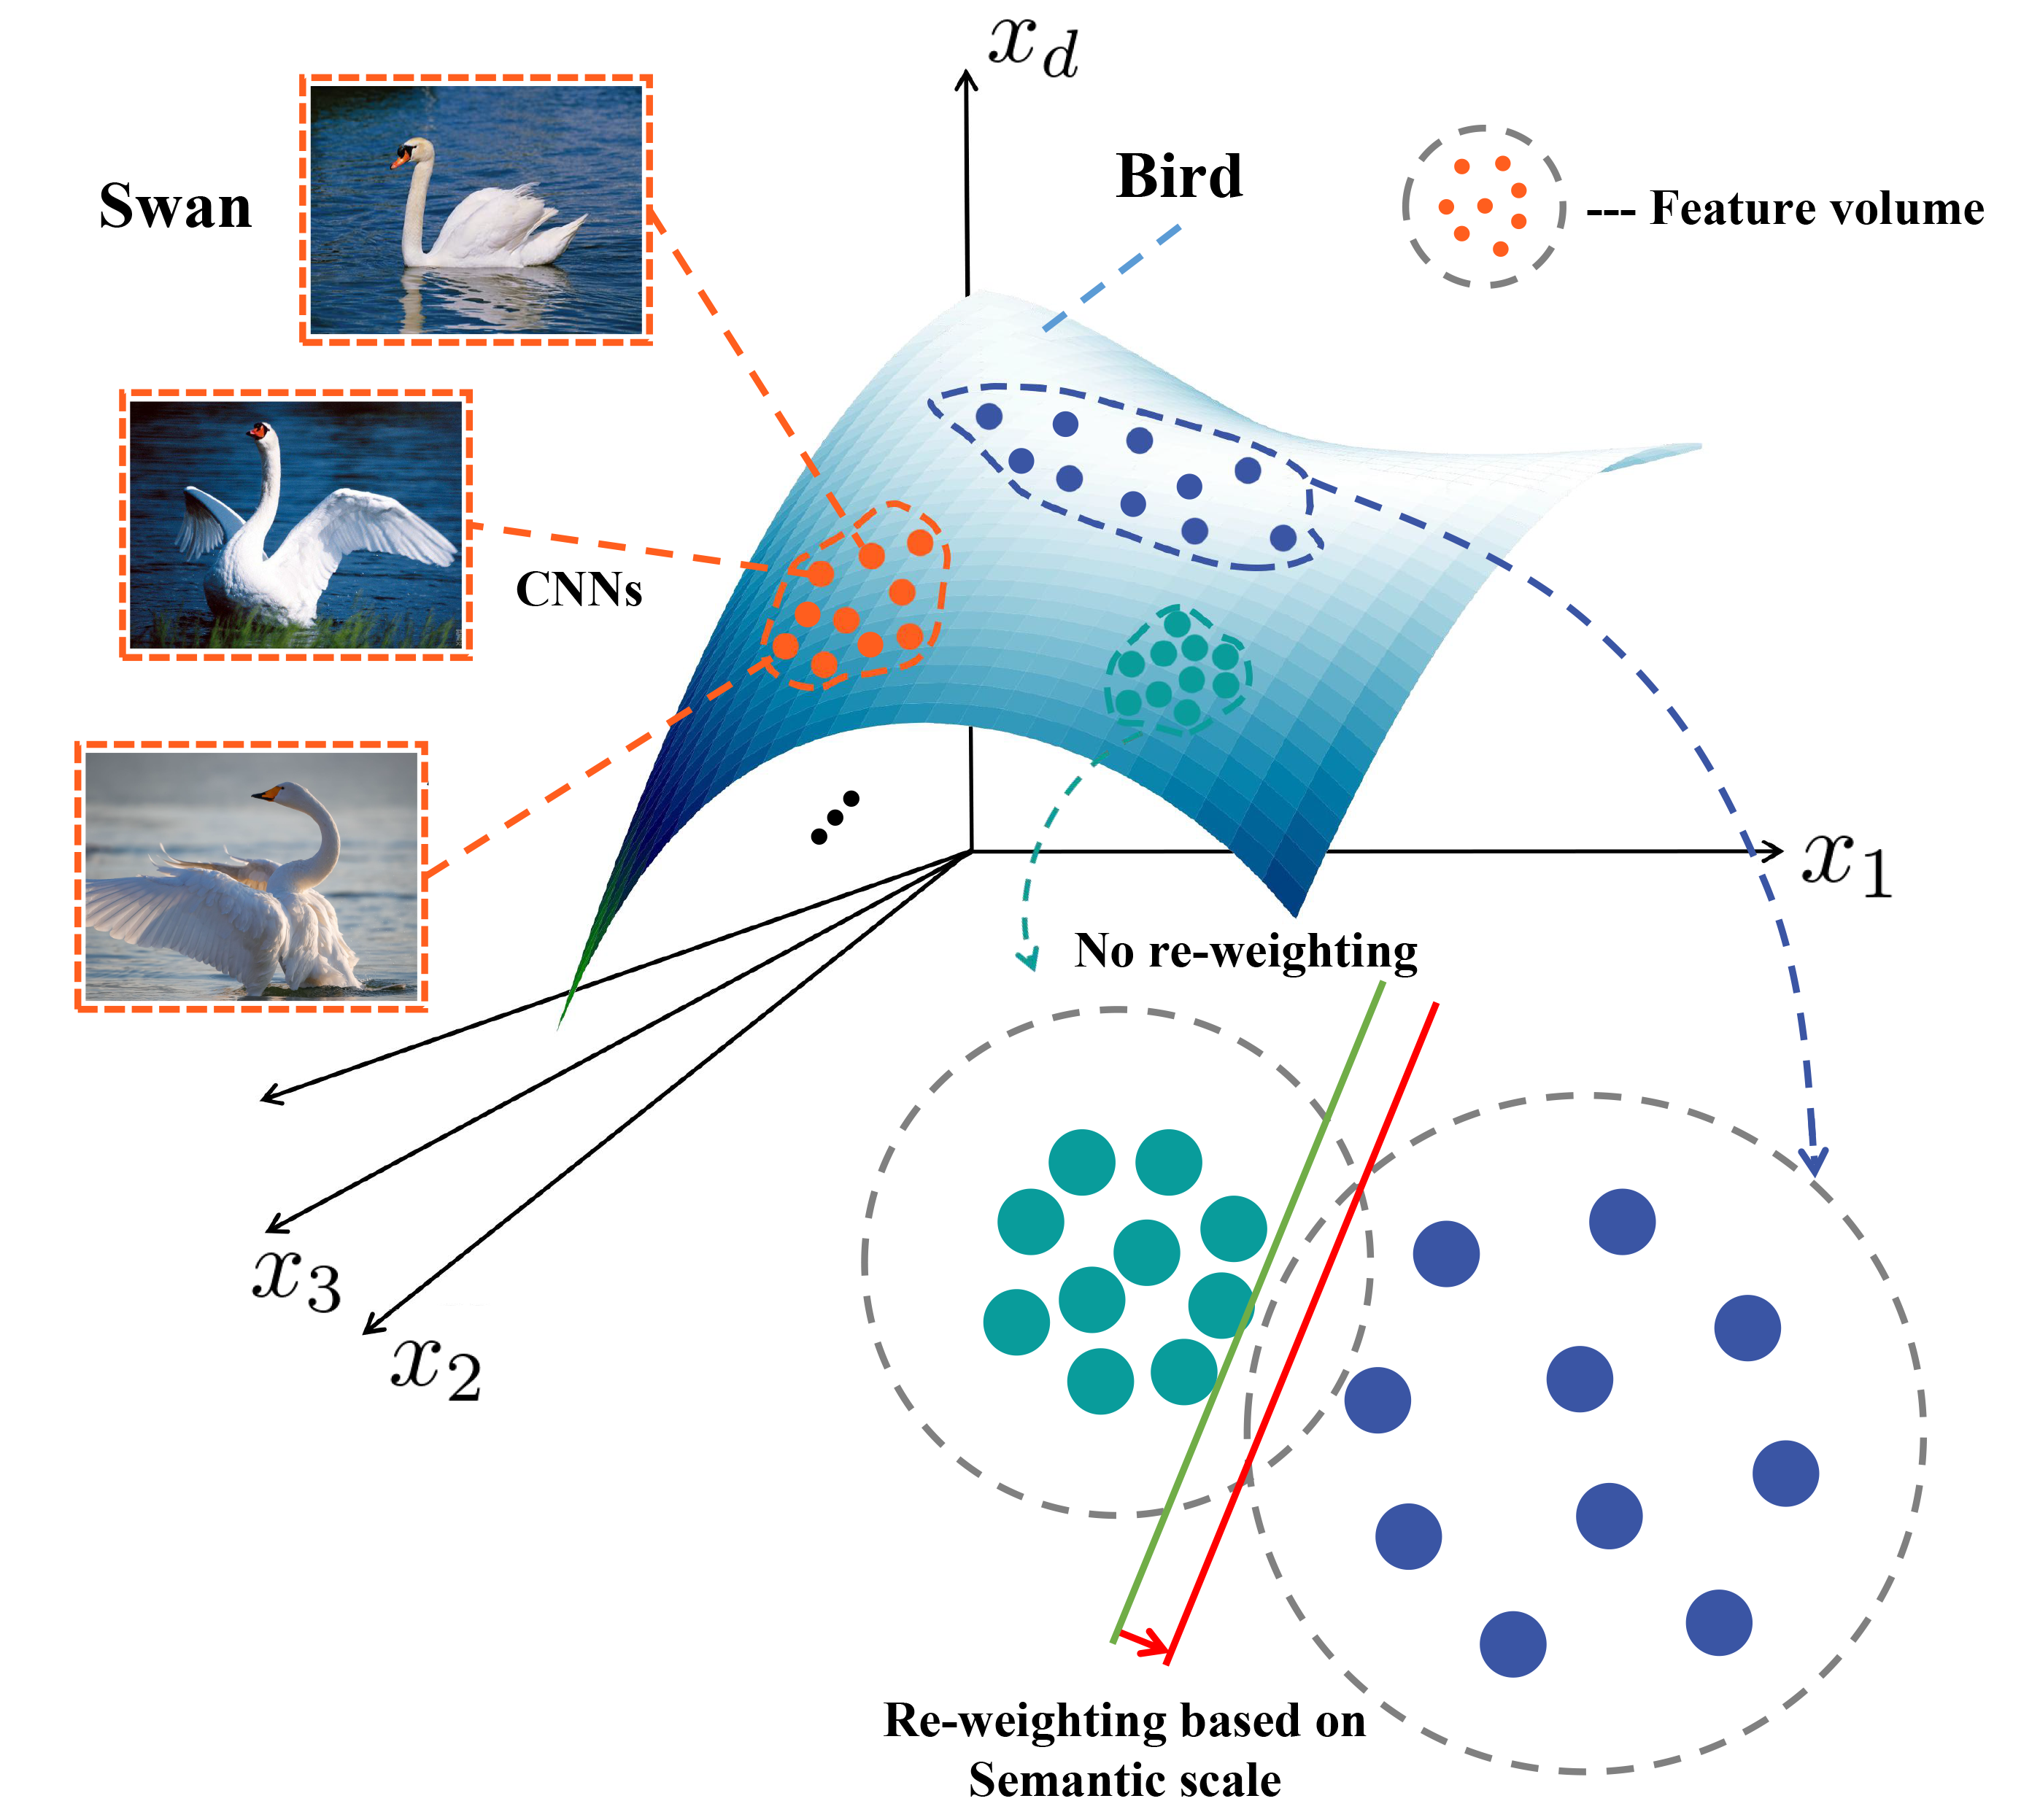
\includegraphics[width=0.45\columnwidth]{fig1}
\vskip -0.1in
\caption{The features from "Bird" mapped by CNNs are concentrated on a low-dimensional manifold, and the three-color point sets represent the three sub-classes of "Bird". Among them, the \textcolor[RGB]{255,94,30}{orange} point set represents "Swan", whose feature volume is obviously smaller than that of "Bird". The classification experiments on sample-balanced datasets show that the models are biased towards the classes with larger semantic scales, such as the decision surface shown by the \textcolor[RGB]{112,173,71}{green} line. In this case, the re-weighting strategy based on the number of samples does NOT work, while our proposed re-weighting approach based on the semantic scale biases the decision surface toward the class with a larger feature volume (\textcolor[RGB]{255,0,0}{red} line).}
%\vskip -0.03in
\label{fig1}
\end{center}
\end{wrapfigure}
%\exercise

The experiments demonstrate that semantic scale imbalance is more widely present in natural datasets than sample number imbalance, allowing the study scope for class imbalance to be extended to arbitrary datasets. Then, how to mitigate the adverse effects of semantic scale imbalance? We are inspired by classification methods for long-tailed data, and current solutions for class imbalance problem usually adopt re-sampling strategies \cite{paper8,paper10,paper12} and cost-sensitive learning \cite{paper16,paper17,paper18}. However, re-sampling may either introduce a large number of duplicate samples, making the model susceptible to overfitting when oversampling, or discard valuable samples when undersampling. Therefore by drawing on the classical re-weighting strategy \cite {paper24}, we propose the dynamic semantic-scale-balanced learning. Its core idea is to dynamically rather than invariably measure the degree of imbalance between semantic scales in the feature space, to achieve a dynamic evaluation of the weaker classes and assign greater weights to their corresponding losses.


In this work, our \textbf{key contributions} are summarized as:


\textbf{(1)} We propose the novel idea of leveraging the volume of manifold to measure the semantic scale (Sec \ref{3.2}). It is also innovative to find that the semantic scale has the marginal effect (Sec \ref{3.3}), and that the semantic scale of the dataset is highly consistent with model performance in terms of trends.

\textbf{(2)} We introduce and define semantic scale imbalance, aiming to measure the degree of class imbalance by semantic scale rather than sample number, which reveals a new perspective for the study of class imbalance problem. Experiments show that semantic scale imbalance is prevalent in the dataset and can more accurately reflect model bias that affects model performance (Sec \ref{3.4}).

\textbf{(3)} Semantic-scale-balanced learning is proposed to mitigate model bias, which includes a general loss improvement scheme (Sec \ref{4.1}) and a dynamic re-weighting training framework (Sec \ref{4.2}) that overcomes the challenge of calculating semantic scales in real-time during iterations. Comprehensive experiments demonstrate that semantic-scale-balanced learning is applicable to a variety of datasets and achieves significant performance gains on multiple vision tasks (Sec \ref{5}).

\section{Slow Drift Phenomenon of Features and Marginal Effect\label{2}}


Since the model parameters are changing during training, \cite {paper25} studies the drifting speed of embeddings by measuring the difference in features of the same instance across training iterations. Experiments on the Stanford Online Products (SOP) dataset \cite {paper83} show that the features change drastically in the early stage of training, become relatively stable after traversing the dataset twice, and drift gets extremely slowly when the learning rate decreases. This ensures that it is reasonable to leverage historical features to calculate semantic scales.

Marginal effect \cite {paper14} describes that in the early stages of model training, the network is able to learn features quickly, but since there is information overlap among samples, as the number of samples increases, the information of data will gradually saturate and the improvement in model performance from newly added samples will diminish. The effective number of samples is proposed to represent the information of data, but its limitation is that it does not work when the number of samples for each class is balanced.

Assume that the volume of each sample is unit volume $1$ and define the set of all samples for a class as $\Omega$ with volume $N$ and $N\!\!\ge\!\!1$. A new sample may overlap with a previous sample such that the probability of overlap is $P$ and that of non-overlap is $1\!\!-\!\!P$. As the information of data increases, the probability $P$ will be higher. 

Define the effective number of samples as ${E_n}$, and ${E_n} = 1 + \beta \frac{{1 - {\beta ^{n - 1}}}}{{1 - \beta }} = \frac{{1 - {\beta ^n}}}{{1 - \beta }}$ \cite {paper14}, where $n$ denotes the number of samples, hyperparameter $\beta = \frac{{N - 1}}{N} \in [ {0,1} )$ controls how fast ${E_n}$ grows as $n$ increases. When $N = 1$, $\beta  = 0$ and ${E_n}= 1$, meaning that all samples can be represented by a single prototype via data augmentation. When $N \to \infty $, $\beta  \to 1$, implying that there is no overlapping, then $\mathop {\lim }\limits_{\beta  \to 1 } \!\!\frac{{1 - {\beta ^n}}}{{1 - \beta }} \!\!= \!\!\mathop {\lim }\limits_{\beta  \to 1 } \!\!\frac{{{{\left( {1 - {\beta ^n}} \right)}^\prime }}}{{{{\left( {1 - \beta } \right)}^\prime }}} \!\!= \!\!\mathop {\lim }\limits_{\beta  \to 1 } \!\!\frac{{ - n{\beta ^{n - 1}}}}{{ - 1}} \!\!= \!\!n$, which indicates that the effective number of samples does not increase faster than the number of samples, but this is not the case in our experimental results.

The effective number of samples ${E_n}$ is an exponential function of the number of samples $n$. The hyperparameters $\beta$ corresponding to classes of different grain should be different. However, the selection of $\beta$ requires more information from the data itself, but this problem is not addressed by \cite {paper14}, which is forced to assume that $\beta$ is the same for all classes. In this case, compared to the number of samples, ${E_n}$ simply uses the exponential function to obtain smoother weights. Furthermore, when the number of samples is balanced, ${E_n}$ is the same for each class and cannot be used to mitigate model bias, so we attempt to mine the data for information (or feature diversity) of each class to facilitate the study of imbalance problem.


\section{Semantic Scale Imbalance}
In this section, first, sample volume, feature volume, and semantic scale imbalance are defined. Next, we derive a quantitative measurement of feature volume to measure the semantic scale from the perspective of singular value decomposition of the data matrix and information theory. Then, the marginal effect of semantic scale is investigated. Finally, we discuss the relationship between semantic scale imbalance and model bias.
\subsection{Definitions}

Different semantic concepts correspond to different semantic scales, for example, the scale of "Bird" is larger than that of "Swan". For each class, we equate its feature diversity to its semantic scale and measure the semantic scale by the volume of subspace spanned by samples or features. Deep neural networks can be viewed as a combination of a feature mapping function $f({x,\theta})$ and a trained downstream classifier $g(z)$, i.e., $x\to z( \theta )\to y$. Let the samples of a class be $X=[ {{x_1},{x_2}, \ldots ,{x_m}} ]$, and the embeddings learned by deep neural networks are represented as $Z = \left\{ {{z_i}|{z_i} = f( {{x_i},\theta } ) \in {\mathbb{R}^d},i = 1,2, \ldots ,m} \right\}$.

\textbf{Definition 3.1.} (Sample volume) The volume of the subspace spanned by sample set $X$.

\textbf{Definition 3.2.} (Feature volume) The volume of the subspace spanned by feature vectors $Z$.

\textbf{Definition 3.3.} (Semantic scale imbalance) A phenomenon of imbalance in the size of semantic scales measured by sample volume or feature volume.



\subsection{Quantification of Semantic Scale\label{3.2}}
Given the data $X=[ {{x_1},{x_2}, \ldots ,{x_m}} ]$ and the learned embeddings $Z = \left[ {{z_1},{z_2}, \ldots ,{z_m}} \right] \in {\mathbb{R}^{d \times m}},{z_i} = f( {{x_i},\theta } ) \in {\mathbb{R}^d},i = 1,2, \ldots ,m$, the volume of subspace spanned by the random vector ${z_i}$ (i.e., the feature volume) is derived below, and the sample volume can be calculated in the same way (Appendix \ref{C}). The covariance matrix of random vector ${z_i}$ is estimated as $ \Sigma = E\!\left[ {\frac{1}{m}\!\sum\limits_{j = 1}^m {{z_j}z_j^T} } \right] = \frac{1}{m}\!Z\!{Z^T} \in {\mathbb{R}^{d \times d}}$, ${\lambda _1} \ge {\lambda _2} \ge  \cdots  \ge {\lambda _d} > 0$ are the eigenvalues of real symmetric matrix. The singular value decomposition (SVD) of $Z$ yields $Z = U\Sigma {V^T}$ and the singular values are ${\sigma _j} = \sqrt {{\lambda _j}} ,j = 1,2, \ldots ,d$. The volume of the space spanned by the vector ${z_i}$ is proportional to the product of all singular values of the feature matrix $Z$, i.e., $V\!ol( Z ) \propto \prod\limits_{j = 1}^d {{\sigma _j}}  = \sqrt {\prod\limits_{j = 1}^d {{\lambda _j}} }$. After the determinant expansion, the characteristic polynomial of the matrix $\Sigma$ is $\Phi ( \lambda ) =  \det ( {\lambda I - \Sigma } ) ={\lambda ^d} - ({{a_{11}}+{a_{22}}+ \cdots {a_{dd}}}){\lambda ^{d - 1}} +  \cdots  + {( { - 1} )^d}\det\! \Sigma$, and ${\lambda _1}{\lambda _2} \cdots {\lambda _d} = \det\! \Sigma $. Therefore, the volume of the space spanned by the vector ${z_i}$ is proportional to the square root of the determinant of the covariance matrix of $Z$:
\begin{equation}
V\!ol( Z ) \propto \sqrt {\det ( {\frac{1}{m}\!Z\!{Z^T}} )}. 
\end{equation}The same result can be derived from the volume of a parallel hexahedron defined by vectors (Appendix \ref{E}). Considering that real-world metric tools typically have a dynamic range, for example, a ruler always has multiple scales (1mm, 1cm, or even 10cm) to measure objects of different scales, we expect the quantitative measurement of feature volume to have a multi-scale metric and therefore use the sphere packing method \cite{paper26,paper27}, which is normally adopted in information theory, to implement it.



There is an error at the boundary when filling with hyperspheres because all spheres cannot be exactly tangent to the edges of the manifold. The error of the finite feature vectors is assumed to be independent additive Gaussian noise \cite{paper26} : ${z_i}^\prime  = {z_i} + {w_i}$, where ${w_i} \sim N( {0,\frac{{{\varepsilon ^2}}}{n}I} )$ (n is the space dimension). The estimate of the number of spheres of radius $\varepsilon$ needed to pack the space spanned by all vectors is ${N_\varepsilon }{\rm{ = }}{{V\!ol\left( {Z'} \right)} \mathord{\left/{\vphantom {{V\!ol\left( {Z'} \right)} {V\!ol\left( w \right)}}} \right.\kern-\nulldelimiterspace} {V\!ol\left( Ball \right)}}$. The adjustment of the metric scale can be achieved by tuning the radius $\varepsilon$ of the spheres, thus controlling the measurement result of feature volume. Then the covariance matrix of the vector ${z_i}$ is $\Sigma ' = \frac{{{\varepsilon ^2}}}{n}I + \frac{1}{m}Z\!{Z^T} \in {\mathbb{R}^{d \times d}}$, such that $V\!ol( {Z'} ) \propto \sqrt {\det ( {\frac{{{\varepsilon ^2}}}{n}I + \frac{1}{m}Z\!{Z^T}} )} $ and $V\!ol( Ball ) \propto \sqrt {\det ( {\frac{{{\varepsilon ^2}}}{n}I} )}$. The feature volume is proportional to ${N_\varepsilon }$:
\begin{equation}
\begin{aligned}
V\!ol\left( Z \right) \propto {N_\varepsilon } &= \frac{{V\!ol\left( {Z'} \right)}}{{V\!ol\left( Ball \right)}} = \sqrt {\frac{{\det \left( {\frac{{{\varepsilon ^2}}}{n}I + \frac{1}{m}Z\!{Z^T}} \right)}}{{\det \left( {\frac{{{\varepsilon ^2}}}{n}I} \right)}}}  \\ 
&= \sqrt {\det \left( {I + \frac{n}{{m{\varepsilon ^2}}}Z\!{Z^T}} \right).} 
\end{aligned}
\end{equation}The dimension of feature ${z_i}$ is $d$, so let $n=d$. In order to increase the numerical stability, we perform a logarithmic transformation of the above equation, which does not affect the monotonicity of the function, and we can obtain $V\!ol\left( Z \right) \propto {\log _2}\sqrt {\det \left( {I + \frac{n}{{m{\varepsilon ^2}}}Z\!{Z^T}} \right)}  = \frac{1}{2}\log \det \left( {I + \frac{d}{{m{\varepsilon ^2}}}Z\!{Z^T}} \right)$. In practical training, it is essential to normalize the feature vectors so that their mean value is $0$. In this work, we set $\varepsilon=1000$, and the value of $\varepsilon$ does not affect the relative size of the space spanned by feature vectors of each class. The volume of the space spanned by $Z$ can be can be written as:
\begin{equation}
V\!ol( Z ) = \frac{1}{2}{\log _2}\det ( {I + \frac{d}{m}( {Z - {Z_{mean}}} ){{( {Z - {Z_{mean}}} )}^T}} ),
\end{equation}

where $Z_{mean}$ is the mean value of $Z$, $V\!ol( Z )>0$ when the number of samples $m>1$. We measure the semantic scale $S'$ by the feature volume, i.e., $S' = V\!ol( Z )$, and the larger $S'$, the richer the feature diversity, which we verify in Appendix \ref{Experiments on Stanford point cloud manifolds} using multiple Stanford point cloud manifolds. 

\subsection{Marginal Effect of Semantic Scale\label{3.3}}

\begin{wrapfigure}[29]{r}{21em} % 纵向8行,图片靠右,宽度12.5em
\begin{center}
\vskip -0.32in
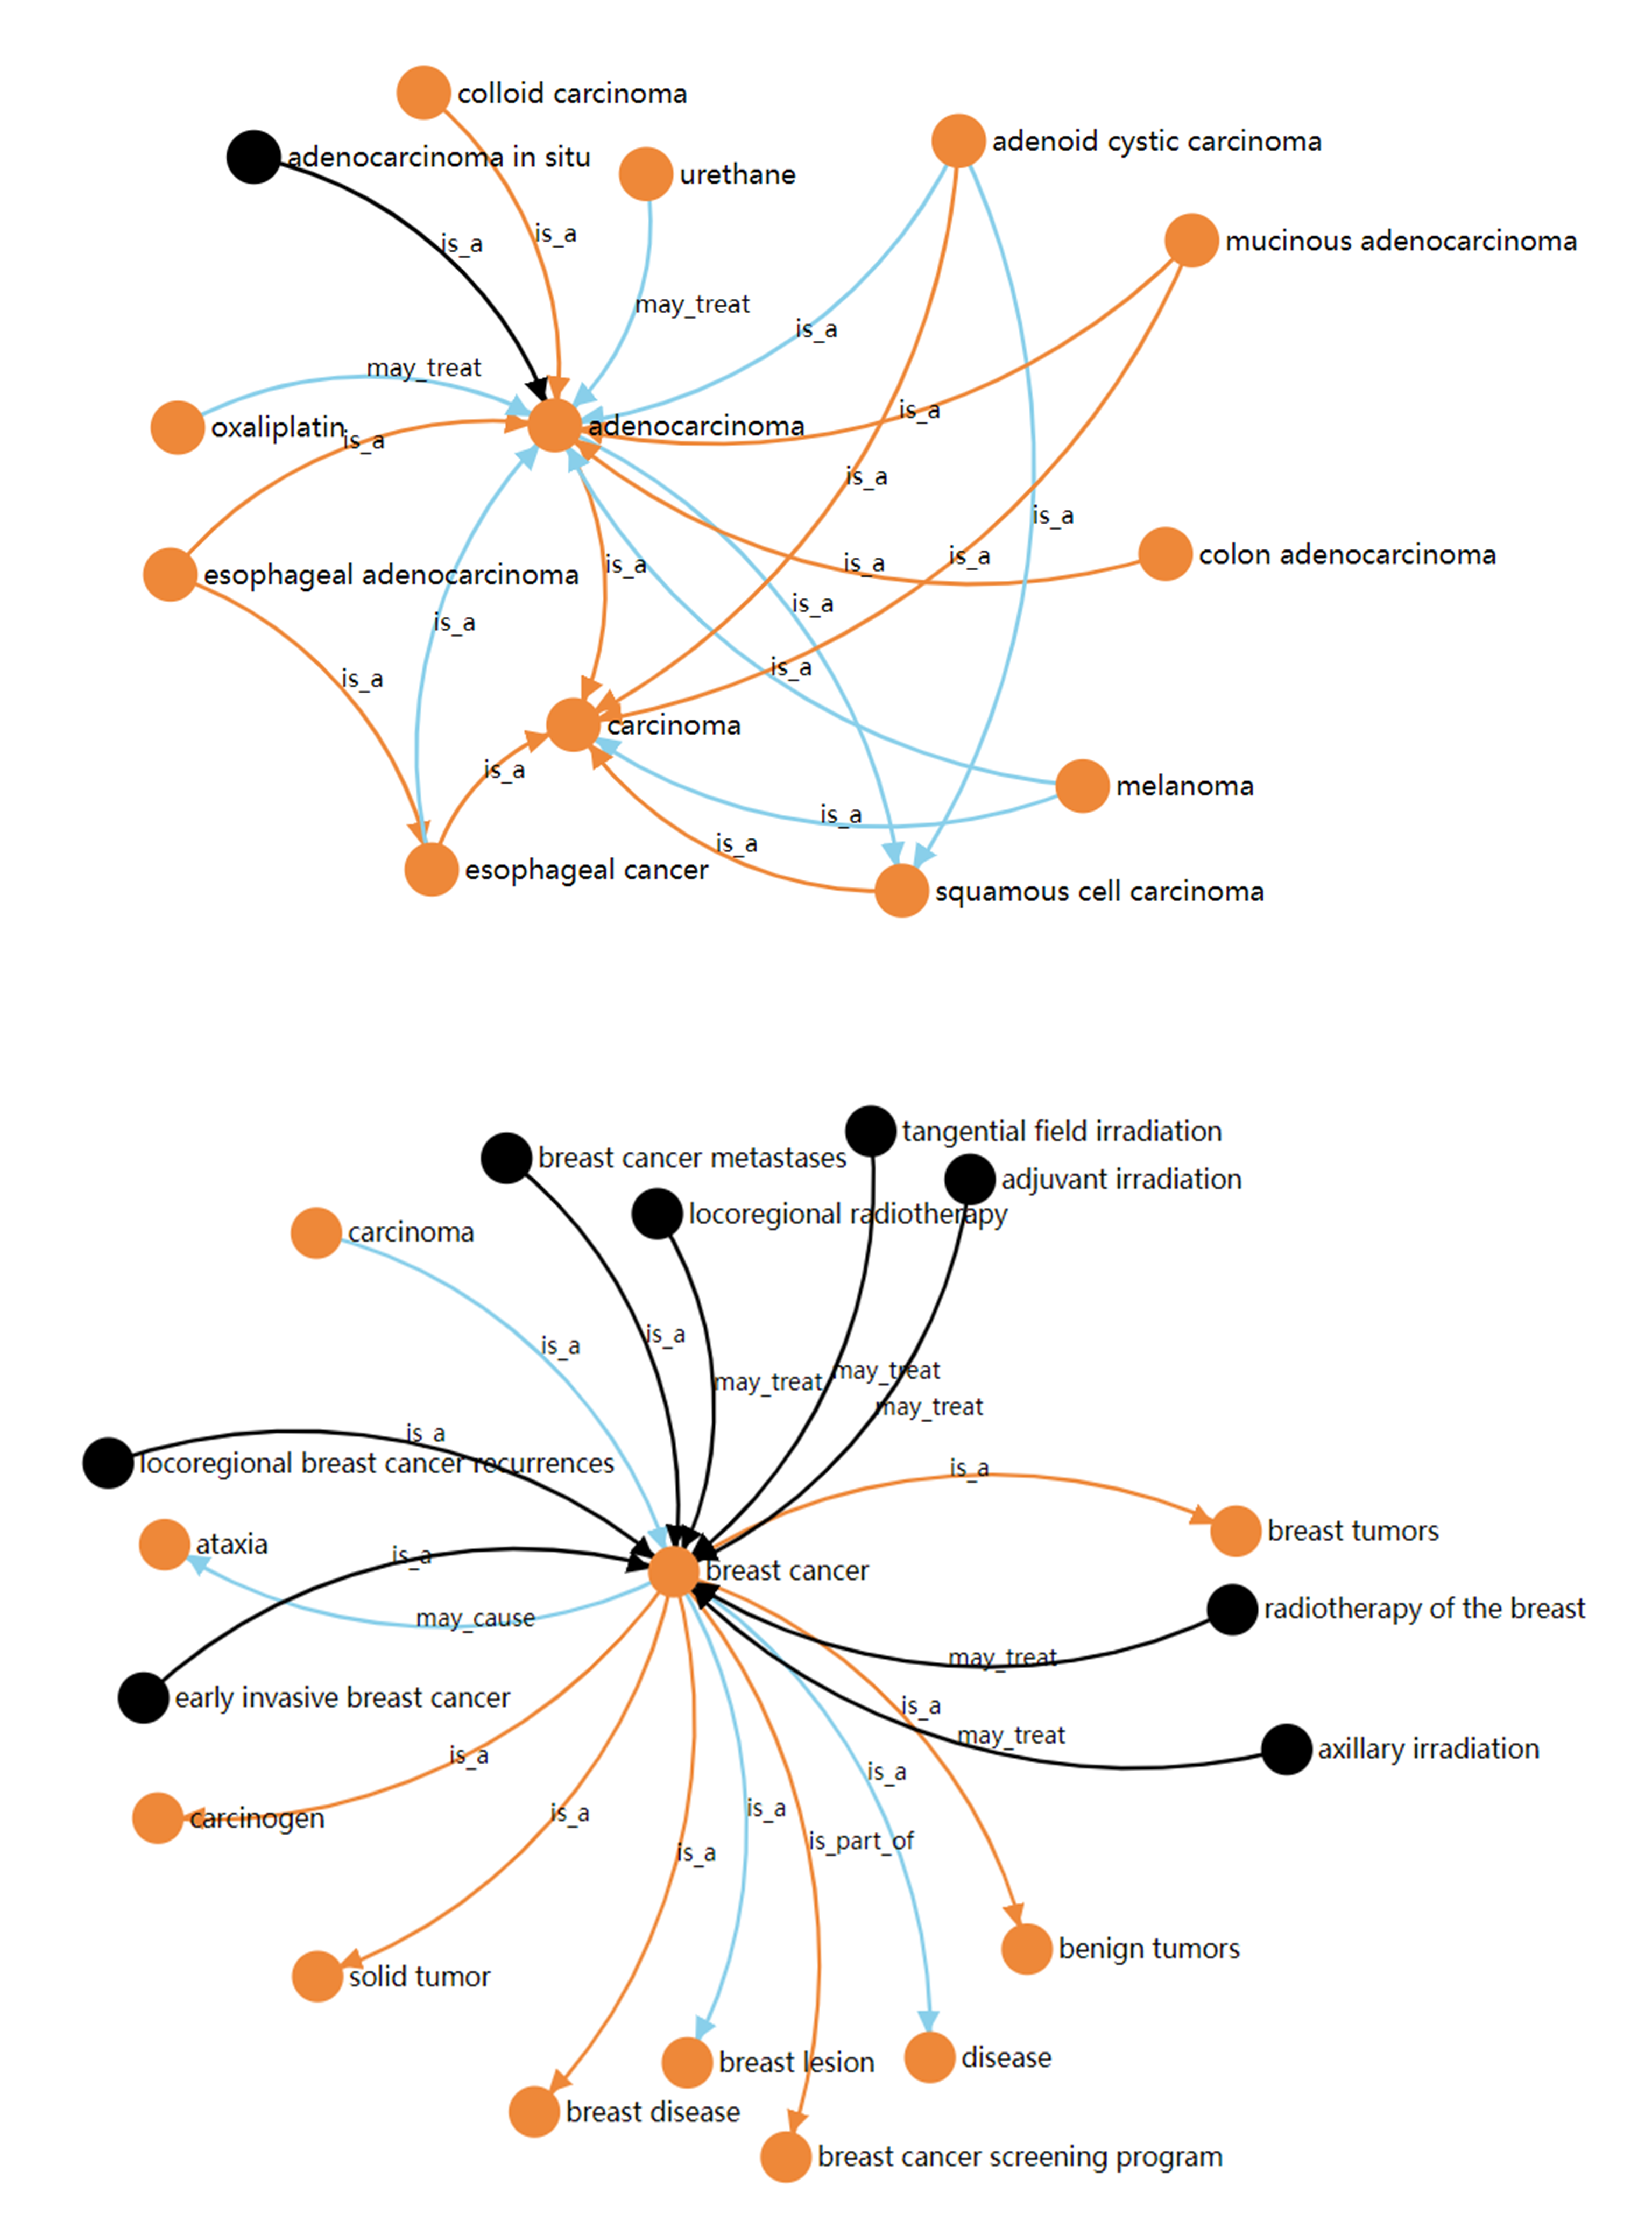
\includegraphics[width=0.47\columnwidth]{figure2}
\vskip -0.14in
\caption{\textbf{Left column}: curves of semantic scales with increasing number of samples for the first ten classes from different datasets. \textbf{Right column}: for different sub-datasets, curves of the sum of semantic scales for all classes and top-1 accuracy curves of trained ResNet-18 and ResNet-34. All models are trained using the Adam optimizer \cite {paper33} with an initial learning rate of 0.01 and then decayed by 0.98 at each epoch.}
\label{fig2}
\end{center}
\end{wrapfigure}
%\exercise

The marginal effect describes that the feature richness will gradually saturate as the number of samples increases, so the change of semantic scale should also conform to the marginal effect. Figure \ref{fig2} illustrates that as the number of samples increases, the semantic scale $S'$ measured by sample volume gradually saturates, which indicates that the quantitative measurement of semantic scale is as expected. In addition, the growth rate of the semantic scale varies across classes, which is determined by the grain size of the class itself. It leads to different semantic scales even if all classes have the same number of samples.

To investigate why adding samples has a marginal improvement in model performance when the training samples are sufficient, we use the following method to generate new training datasets for classification experiments: assume that the total number of classes in the original dataset is $C$, and $m$ samples are randomly selected from each class to form a sub-dataset with a total number of samples of $C \times m$. The sub-datasets generated based on CIFAR-10, CIFAR-100 \cite {paper28} and Mini-ImageNet \cite {paper31} are shown in Appendix \ref{B.1}.


We train ResNet-18 and ResNet-34 \cite {paper32} on each of the \textbf{31} training sets in Table \ref{table6}, and the sum of the semantic scales for all classes and the corresponding top-1 accuracy are shown in Figure \ref{fig2}. We are pleasantly surprised to find that when the semantic scale increases rapidly, the model performance improves swiftly with it, and when the semantic scale becomes saturated, the improvement is small.


\subsection{Semantic Scale Imbalance and Model Bias \label{3.4}}
\subsubsection{Quantification of Semantic Scale Imbalance}

\begin{table}[h]
\renewcommand\arraystretch{1.3}
\vskip -0.15in
\setlength{\tabcolsep}{6pt} %修改边距
\caption{Pearson correlation coefficients between the accuracy of classes and the semantic scales $S$ with different $\alpha$. $N$ denotes the number of samples, and $S'$ represents the semantic scale without considering inter-class interference. $E_n$ denotes the number of effective samples.}
\label{table1}
\vskip 0.03in
\centering  
\begin{small}
\begin{tabular}{l|c|c|c|c|c|ccccc }
\hline \toprule
\multirow{2}{*}{Dataset}    & \multirow{2}{*}{Model}   & \multirow{2}{*}{$N$} & \multirow{2}{*}{$E_n$} & \multirow{2}{*}{$W$}  &  \multirow{2}{*}{$S'$}  &\multicolumn{5}{c}{$S$}   \\ \cline{7-11}
       & & & & & &$\alpha$=1  &$\alpha$=1.5  &$\alpha$=2   &$\alpha$=2.5   &$\alpha$=3 \\  \hline
\multirow{2}{*}{CIFAR-10-LT}  & ResNet-18 & 0.8346 &0.8664 &0.2957 & 0.8688 & 0.8456 & \textbf{0.9603} & 0.9553  & 0.9398 & 0.9269 \\
  & ResNet-34 & 0.7938 &0.8476 &0.3186 & 0.9426 & 0.7950 & 0.9678  & \textbf{0.9884} & 0.9854 & 0.9796 \\  \hline
\multirow{2}{*}{CIFAR-10} & ResNet-18 & 0.0950 &0.0950 & 0.1743 & 0.5433 &\textbf{0.7850} & 0.7250  & 0.6644 & 0.6060 & 0.5607 \\
  & ResNet-34 & 0.1502 &0.1502 & 0.2075 & 0.5750 & \textbf{0.8056} & 0.7442 & 0.6870  & 0.6465 & 0.5906 \\
\bottomrule \hline
 \end{tabular}
 \end{small}
\vskip -0.05in
\end{table}

The previous subsection shows that the sum of semantic scales for all classes in the dataset is highly correlated with the model performance, and we further investigate the relationship between semantic scale and model bias for different classes. When a class is closer to other classes, the model performs worse on that class \cite{paper34,paper44}. Therefore, inter-class interference is additionally considered when quantifying the degree of imbalance between semantic scales of classes. When class $i$ is closer to other classes, a smaller weight ${w_i}$ is applied to the semantic scale of class $i$.


Specifically, the semantic scale of $m$ classes after maximum normalization is assumed to be $S' = {\left[ {{S'_1},{S'_2}, \ldots ,{S'_m}} \right]^T}$, and the centers of all classes are $O = {\left[ {{o_1},{o_2}, \ldots ,{o_m}} \right]^T}$. Define the distance between the centers of class $i$ and class $j$ as ${d_{i,j}} = {\left\| {{o_i} - {o_j}} \right\|_2}$, the weight ${w_i} = \frac{1}{{m - 1}}\sum\nolimits_{j = 1}^m {{{\left\| {{o_i} - {o_j}} \right\|}_2}} $. The weights of $m$ classes are written as $W' = {\left[ {{w_1},{w_2}, \ldots ,{w_m}} \right]^T}$. After the maximum normalization and logarithmic transformation of $W'$, we can obtain $W{\rm{ = }}{\log _2}\left( {\alpha  + W'} \right),\alpha  \ge 1$, where $\alpha$ is used to control the smoothing degree of $W$. After considering the inter-class distance, the semantic scale $S = S' \odot W$, and the role of $S'$ in dominating the degree of imbalance is greater when $\alpha$ is larger. 


To obtain the most appropriate $\alpha$, we calculate the Pearson correlation coefficients between the semantic scale and the accuracy of ResNet-18 and ResNet-34 trained on CIFAR-10-LT and CIFAR-10, as shown in Table \ref{table1}. The experimental settings are in Appendix \ref{B.2}. It can be found that $S'$ is more dominant on long-tailed data than on non-long-tailed data, and the improved $S$ is better than $S'$ and far better than the number of samples in reflecting model bias. In the following experiments, we let $\alpha$ be 2 on the long-tailed data and 1 on the non-long-tailed data.

%\vspace{-2mm}
\subsubsection{Semantic Scale Imbalance on Long-Tailed Data}

\begin{wrapfigure}[33]{r}{19.5em} % 纵向8行,图片靠右,宽度12.5em
\begin{center}
\vskip -0.28in
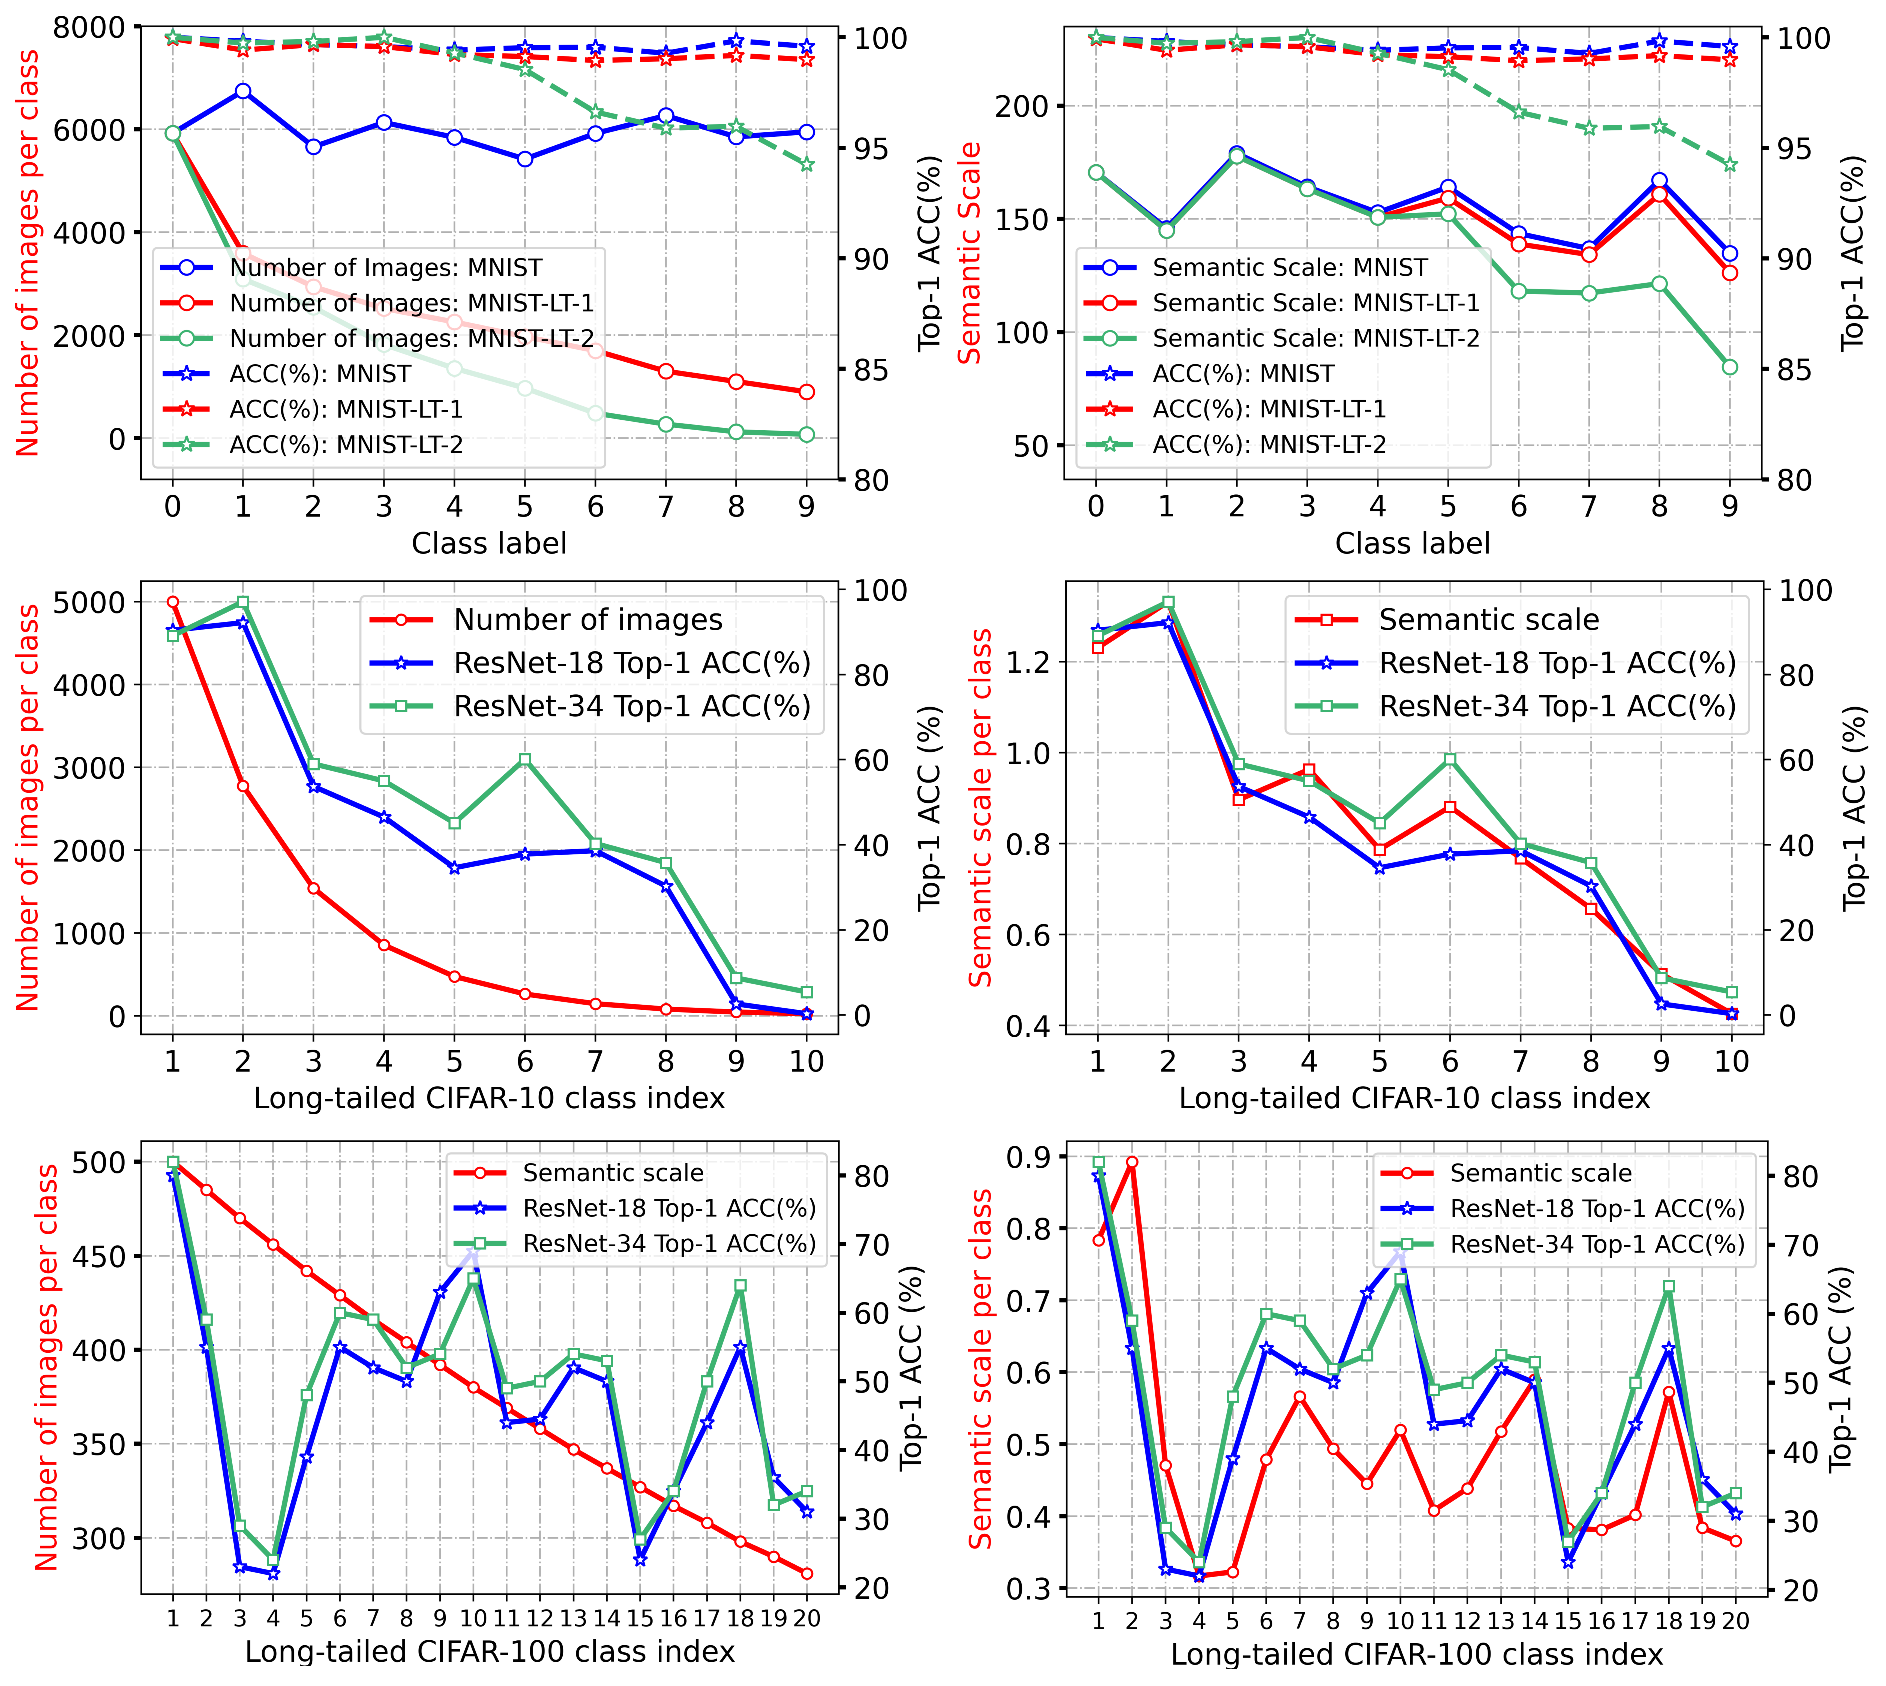
\includegraphics[width=0.43\columnwidth]{3.1}
\vskip -0.1in
\caption{Correlation study of accuracy with the number of samples and semantic scale on MNIST, MNIST-LT (Appendix \ref{B.3}), CIFAR-10-LT and CIFAR-100-LT datasets.}
\label{fig3}

\vskip 0.1in
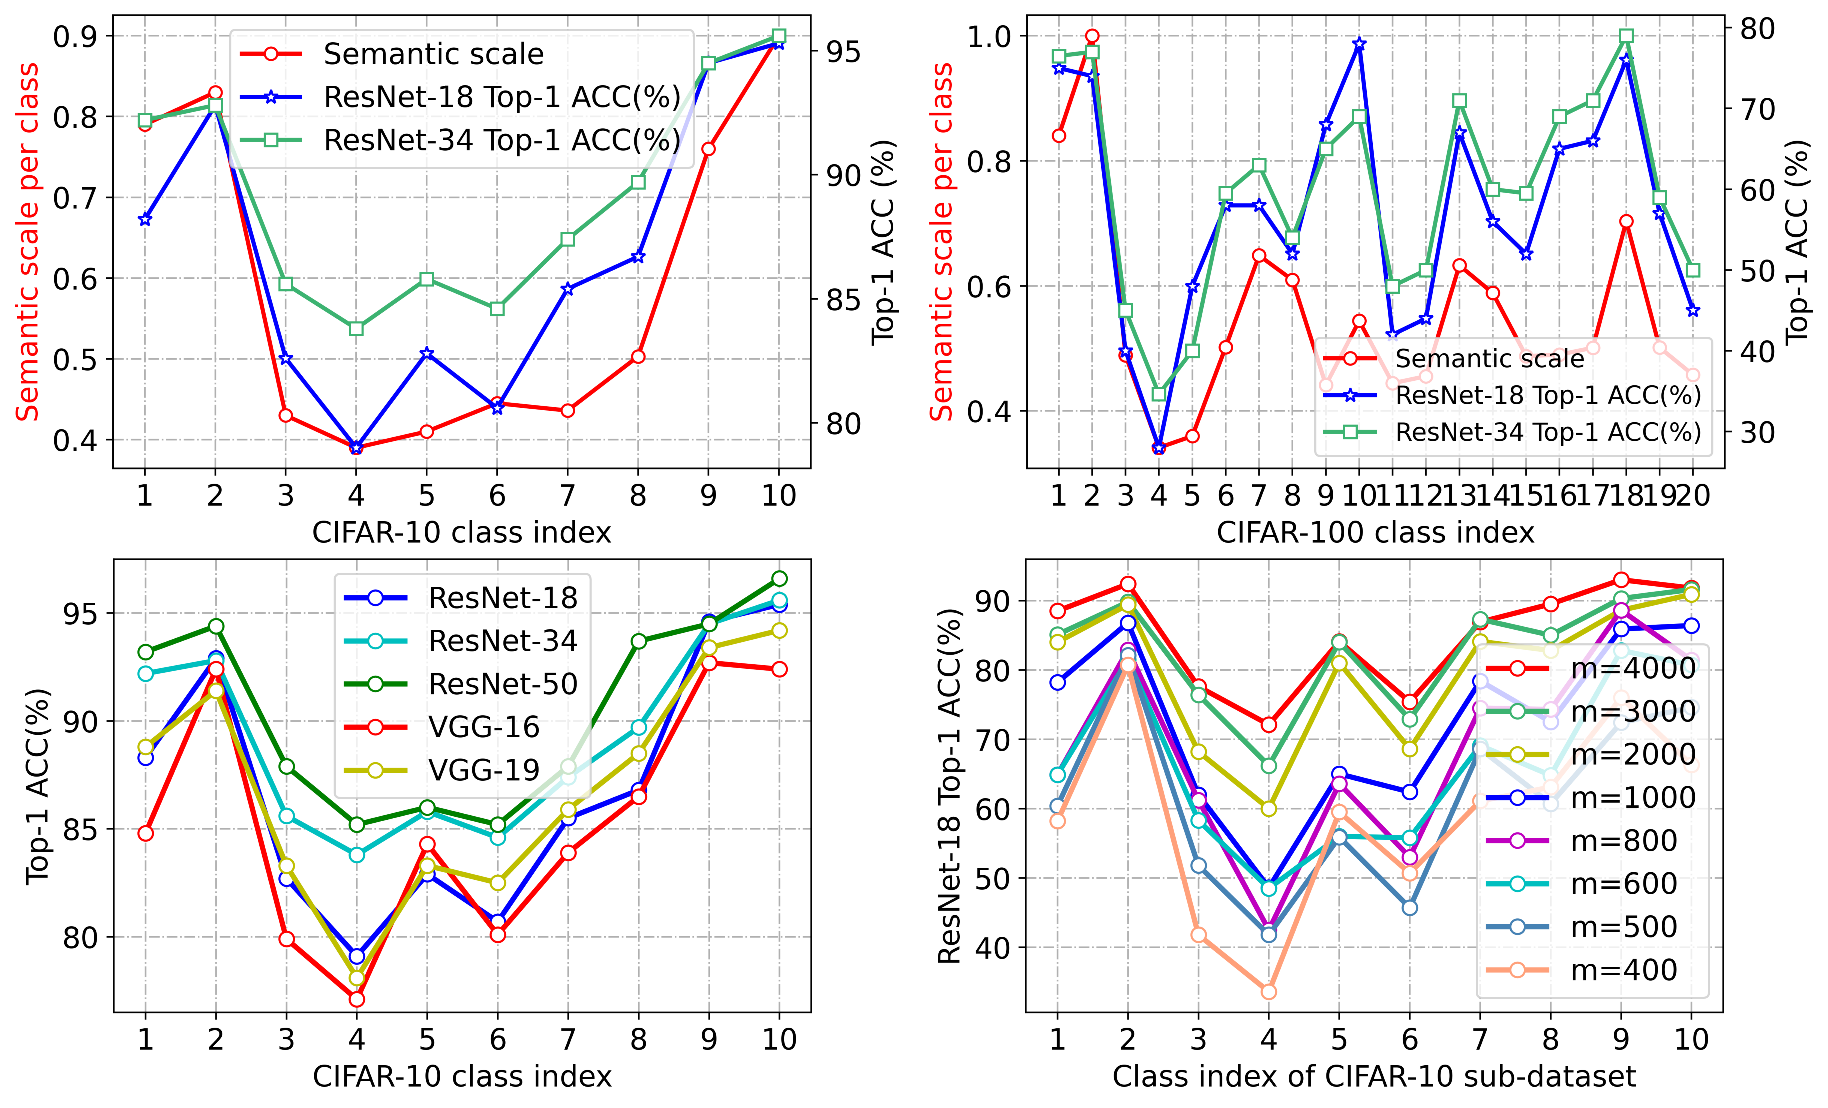
\includegraphics[width=0.43\columnwidth]{n3.2}
\vskip -0.1in
\caption{\textbf{Top row}: correlation study between accuracy and semantic scale on the sample-balanced dataset. \textbf{Bottom row}: performance of different models \cite{paper9} trained on the CIFAR-10 dataset and performance of ResNet-18 trained on different sub-datasets of CIFAR-10 from Table \ref{table6} of Appendix \ref{B.1}.}
\label{fig4}

\end{center}
\end{wrapfigure}
%\exercise

Previous studies have roughly attributed model bias to the imbalance in the number of samples. The experimental results in the first row of Figure \ref{fig3} show that even though the number of MNIST-LT-1 is similar to that of MNIST-LT-2, the class-wise accuracy on MNIST-LT-1 is closer to that on MNIST, just as their semantic scales are also more similar.

In addition, Figure \ref{fig3} indicate that models on certain classes with fewer samples outperform those on classes with more samples, and that the semantic scale $S$ reflects model bias more accurately. Further, we also observe that the accuracy of the CIFAR-100-LT does not show a significant decreasing trend, which can be explained by the marginal effect of the semantic scale (Sec \ref{3.3}).


%\vspace{-2mm}
\subsubsection{Semantic Scale Imbalance on Non-Long-Tailed Data}


Figure \ref{fig4} demonstrates the model bias not only on long-tailed data but also on sample-balanced data. Usually, the classes with smaller semantic scales have lower accuracies. Depending on the size of the semantic scale, it can make it possible for the weaker and dominant classes to be well differentiated. It should be noted that the weaker classes are not random, and experiments in Figure \ref{fig4} show that the models always perform worse on the same classes. More semantic scale imbalance of the datasets is shown in Appendix \ref{B.4}. In summary, semantic scale imbalance can represent model bias more generally and appropriately, and further, we expect to improve the overall performance of the model when facing the semantic scale imbalance problem. Therefore, we propose the dynamic semantic-scale-balanced learning by drawing on the re-weighting strategy.



\section{Dynamic Semantic-Scale-Balanced Learning\label{4}}
Deep neural networks can be viewed as a combination of the feature mapping function and the classifier, and several studies have shown that model bias is mainly caused by classifier bias \cite{paper10,paper11,paper75}, so we are more concerned with semantic scale imbalance in the feature space, i.e., semantic scale measured by the \textbf{feature volume}. In this section, we propose a general semantic-scale-based loss improvement scheme and design a training framework for the successful application of the scheme.


\subsection{Dynamic Semantic-Scale-Balanced Loss\label{4.1}}

During training, the feature vectors corresponding to the samples vary with the model parameters, and thus the semantic scale per class is constantly changing. Compared with the traditional re-weighting strategy, we propose to calculate the degree of imbalance between semantic scales in real-time at each iteration in order to dynamically evaluate the weaker classes and assign greater weights to their corresponding losses. Specifically, for class $i$ at each iteration, normalized re-weighting terms ${\alpha _i} \propto \frac{1}{{{S_i}}},\sum\limits_{i = 1}^C {{\alpha _i}} = 1$, inversely proportional to the semantic scales that take into account inter-class interference, are introduced, and $C$ is the total number of classes. Given the embedding $z$ of a sample and label $y_{i}$, the dynamic semantic-scale-balanced (\textbf{DSB}) loss can be expressed as $D\!S\!B( {z,{y_i}} ) = \frac{1}{{{S_i}}}L( {z,{y_i}} ),i = 1,2, \ldots ,C,$ where ${y_i}$ is the label of the sample from class $i$. How to combine general loss to generate DSB loss is described in Appendix \ref{D.1}. Our approach has great potential to improve the methods of re-balancing loss and adjusting sampling rate based on the number of samples, because both the semantic scale and the number of samples are natural measures and they are not model-dependent.

However, the number of samples used at each iteration is limited, and it is not possible to obtain the features of all samples for calculating the semantic scales. Therefore, we propose a dynamic re-weighting training framework that enables DSB loss to be successfully applied.

\subsection{Dynamic Re-Weighting Training Framework\label{4.2}}

Inspired by the slow drift phenomenon of features \cite {paper25,paper72}, we design a storage pool $Q$ to store and update historical features and propose a three-stage training framework. A mini-batch of features can be dynamically updated at each iteration, and the semantic scale of each class is calculated using all the features in the storage pool. The three-stage training framework is shown in Figure \ref{fig7} and Algorithm \ref{alg2} (More details are in Appendix \ref{D.2}), with the following textual description.

\textbf{(1)} In the \textbf{first stage}, all the features and labels generated by the 1st epoch are stored in $Q$, but they cannot be used directly to calculate semantic scales due to the large drift of historical features from current features in the early stage.

\begin{wrapfigure}[14]{r}{25.2em} % 纵向8行,图片靠右,宽度12.5em
\begin{center}
\vskip -0.3in
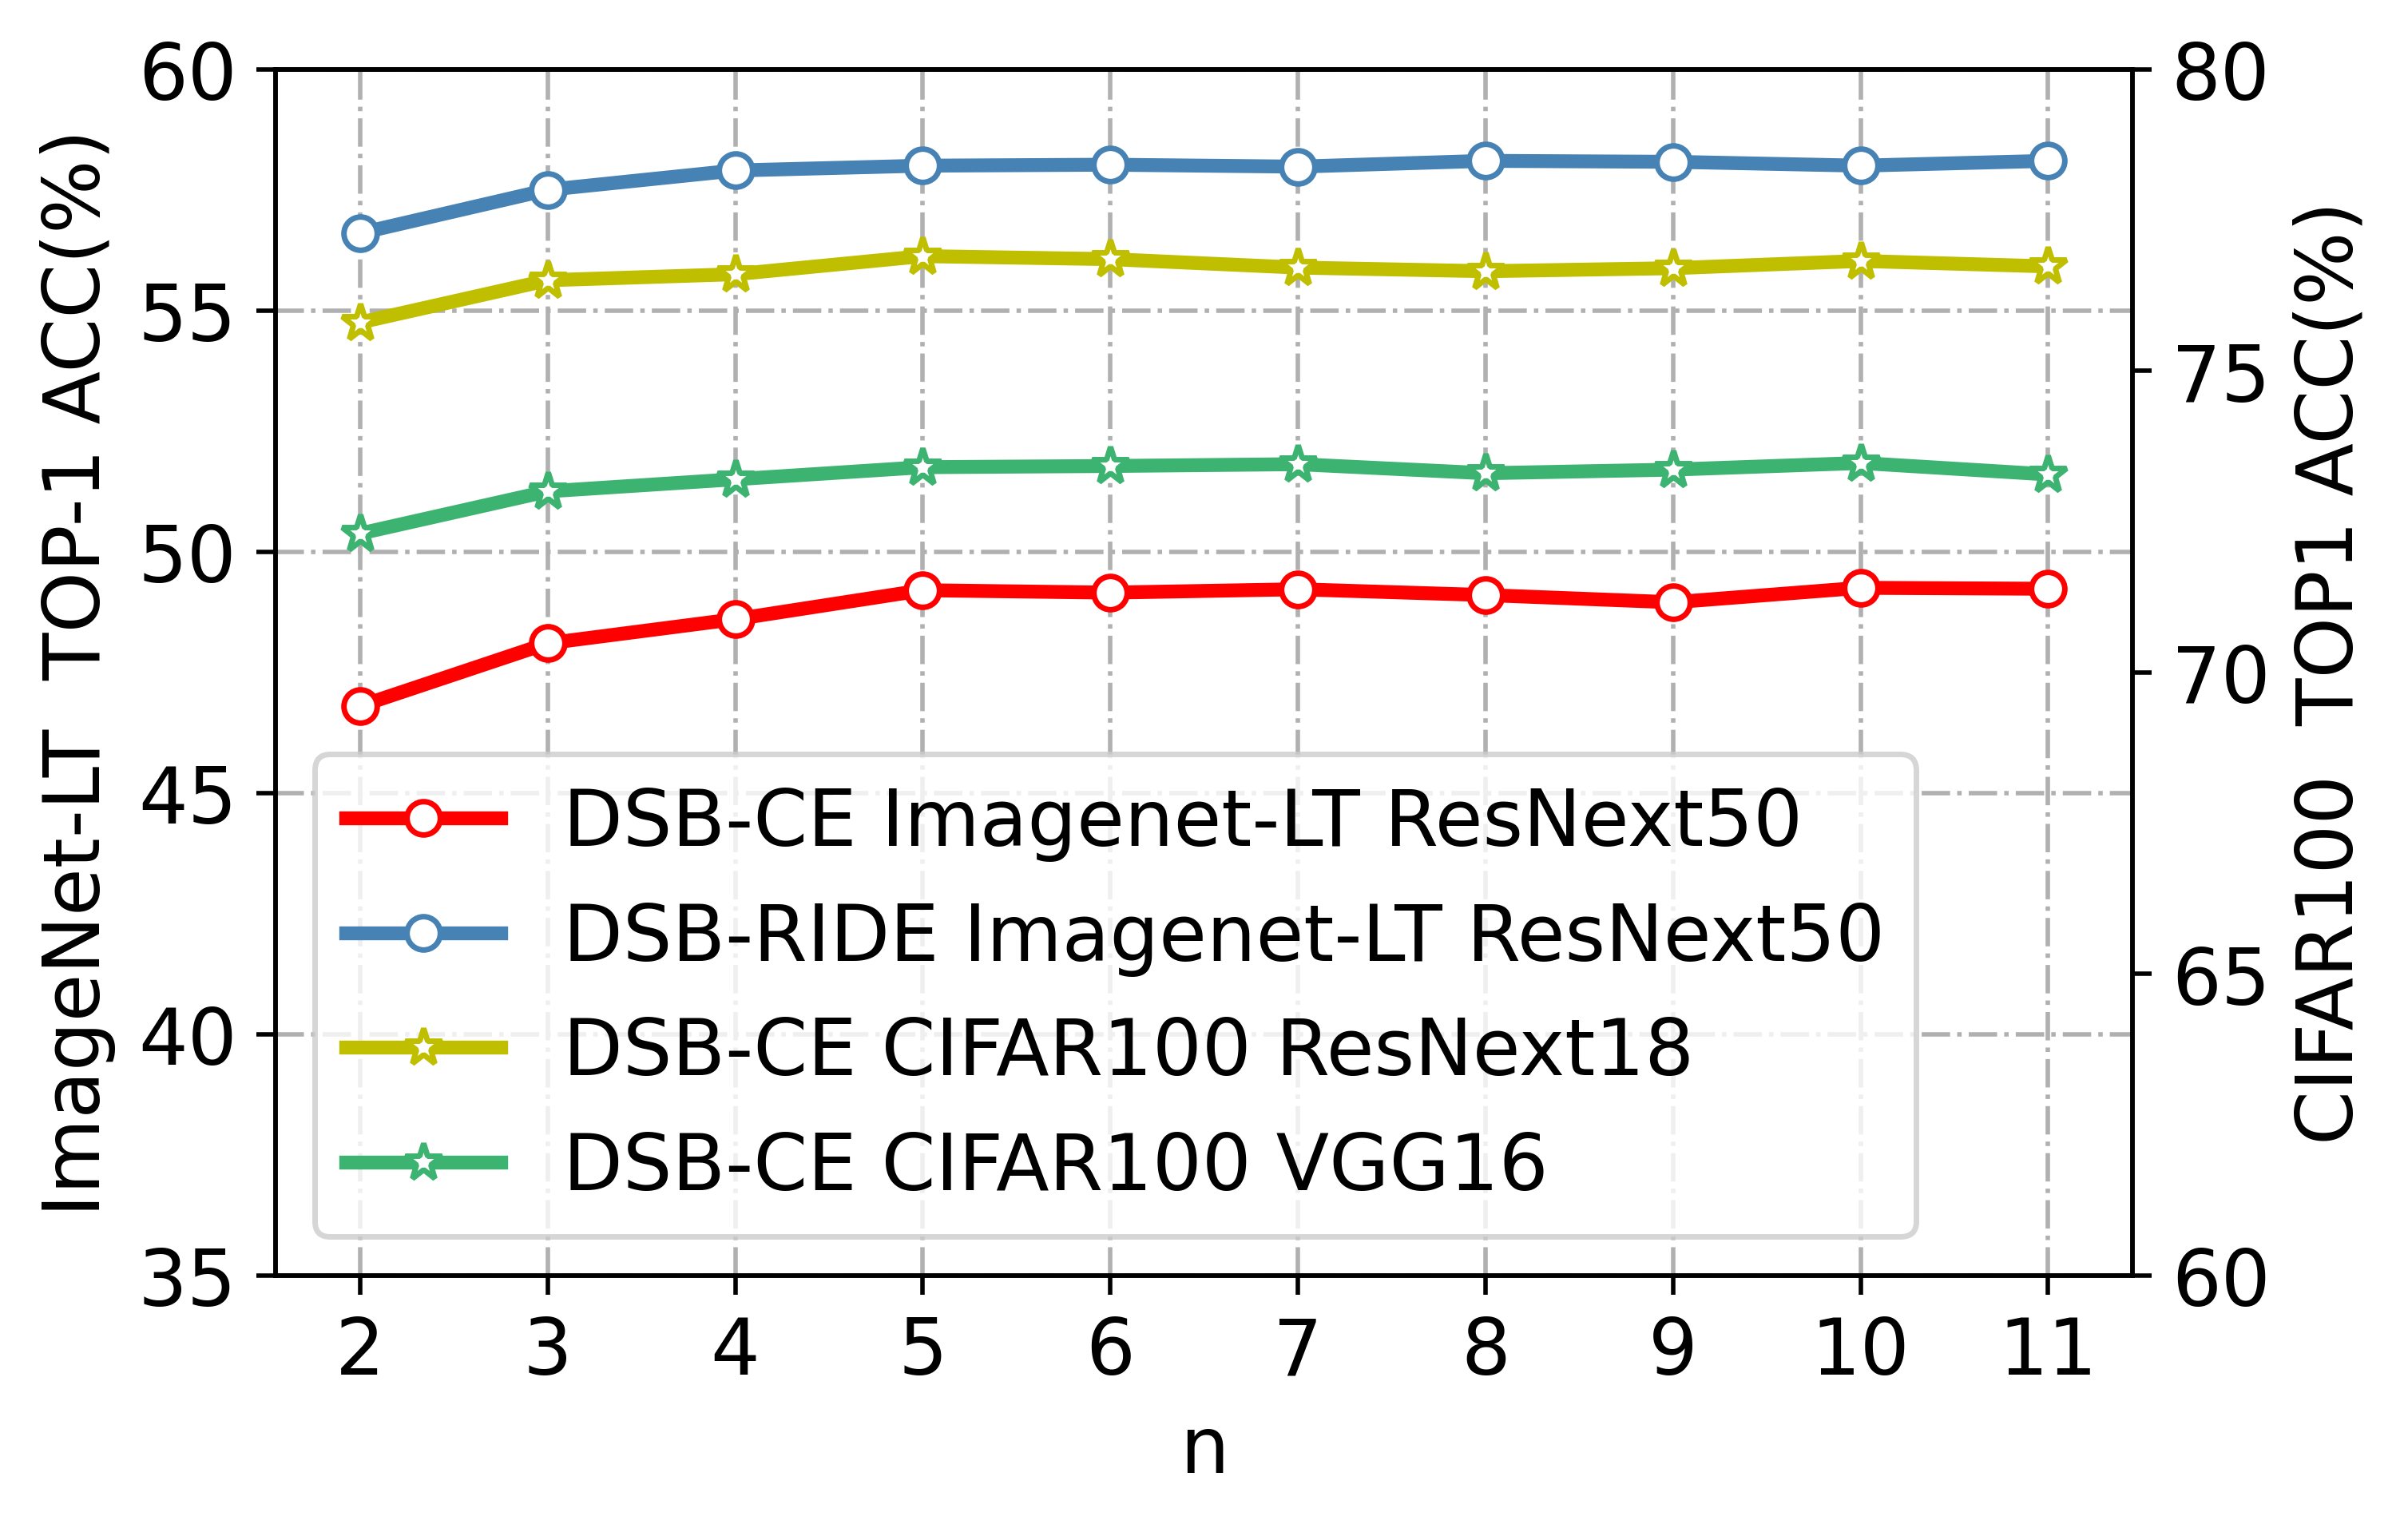
\includegraphics[width=0.52\columnwidth]{fig8}
\vskip -0.25in
\caption{The performance of different models with different losses on different datasets for different values of $n$.}
\label{fig8}
\end{center}
\end{wrapfigure}
%\exercise


\textbf{(2)} The \textbf{second stage} corresponds to epoch 2 to epoch $n$. At each iteration, the oldest mini-batch features and labels in $Q$ are removed and those generated by the current iteration are stored. The goal is to continuously update the features in $Q$ until the feature drift is small enough. We set $n$ to 5 in our experiments, and the original loss function is used in the first two stages. Figure \ref{fig8} shows the effect of $n$ on the model performance. A larger $n$ does not hurt the model performance, but only takes a little more time. Experience suggests that setting $n$ to 5 is sufficient. 

\textbf{(3)} The \textbf{third stage} corresponds to epoch $>$ $n$. At each iteration, the semantic scales are calculated using the features in $Q$ after updating $Q$, and the original loss is re-weighted. 

The comparison and analysis of the \textbf{video memory} and \textbf{training speed} are in Appendix \ref{D.2}. We answer possible questions about the methods section in detail in Appendix \ref{Explanation of a few key points of this paper}.

\section{Experiments\label{5}}

To validate the superiority and generality of the proposed dynamic semantic-scale-balanced learning, we design four experiments. The \textbf{first experiment} is conducted on large-scale long-tailed datasets, ImageNet-LT and iNaturalist2018 \cite {paper67}, to confirm the superior performance of our approach on long-tailed data. The \textbf{second experiment} uses large-scale ImageNet \cite {paper66} and sample-balanced CIFAR-100, and the \textbf{third experiment} selects CIFAR-100-LT and benchmark datasets commonly used in deep metric learning (CUB-2011 \cite {paper29} and Cars196 \cite {paper30}). The \textbf{fourth experiment} is performed on MSCOCO-GLT \cite{paper115} to demonstrate the effectiveness of our approach in generalized long-tailed classification. The comprehensive experiments demonstrate the generality and superiority of our proposed method. More experimental results are provided in Appendix \ref{B.5}, Appendix \ref{B.6} (\textbf{Results on the fundus dataset OIA-ODIR} \cite {paper109}) and Appendix \ref{B.7} (\textbf{Remote sensing image scene classification}). The ablation experiments and additional analyses are in Appendix \ref{H}.

%More experimental results and a comparison of \textbf{memory consumption} and \textbf{training speed} are provided in Appendix B.7.


\subsection{Results on ImageNet-LT and iNaturalist2018 \label{5.1}}

ImageNet-LT is a long-tailed version of ImageNet containing 1,000 classes with between 1,280 and 5 samples per class. iNaturalist2018 is a real-world, extremely unbalanced dataset containing 437,513 images from 8,142 classes. We adopt the official training and validation splits \cite{paper14}.

\begin{table}[h]
\small
\renewcommand\arraystretch{1}
\vskip -0.15in
\setlength{\tabcolsep}{4.9pt} %修改边距
\caption{Top-1 Acc(\%) on ImageNet-LT and iNaturalist2018. We use ResNext-50 \cite {paper81} on ImageNet-LT and ResNet-50 \cite {paper32} on iNaturalist2018 as the network backbone for all methods. And we conduct model training with the SGD optimizer based on batch size 256 (for ImageNet-LT) / 512 (for iNaturalist), momentum 0.9, weight decay factor 0.0005, and learning rate 0.1 (linear LR decay).}
\vskip 0.05in
\label{table2}
\centering  
%\begin{scriptsize}
%\resizebox{.95\columnwidth}{!}{
\begin{tabular}{l|cccc| cccc }
\hline \toprule
\multirow{2}{*}{Methods}    & \multicolumn{4}{c}{ImageNet-LT(ResNeXt50)}  & \multicolumn{4}{|c}{iNaturalist 2018(ResNet50)}  \\ \cline{2-9}
&Head   &Middle   &Tail   &Overall   &Head   &Middle   &Tail   &Overall \\  \hline
BBN \cite {paper10} &43.3 & 45.9 & 43.7 & 44.7 & 49.4  & 70.8 & 65.3 & 66.3 \\
DIVE \cite {paper74} & 64.1 & 50.4 & 31.5 & 53.1 & 70.6  & 70 & 67.6 & 69.1 \\  \hline
CE &65.9 & 37.5 & 7.70 & 44.4 & 67.2  & 63.0 & 56.2 & 61.7 \\
CB-CE \cite {paper14} &39.6 & 32.7 & 16.8 & 33.2 & 53.4  & 54.8 & 53.2 & 54.0 \\
\textbf{DSB-CE} &\textbf{67.3} & \textbf{42.5} &\textbf{21.4}(\textcolor[RGB]{0,201,87}{\textbf{+13.7}}) & \textbf{49.2}(\textcolor[RGB]{0,201,87}{\textbf{+4.8}}) & \textbf{68.5}  & \textbf{63.4} & \textbf{62.7}(\textcolor[RGB]{0,201,87}{\textbf{+6.5}}) & \textbf{64.3}(\textcolor[RGB]{0,201,87}{\textbf{+2.6}}) \\ 
\textcolor{red}{\textbf{DSB-CE+IFL}} \cite{paper115} &\textbf{68.1} & \textbf{43.4} &\textbf{22.5}(\textcolor[RGB]{0,201,87}{\textbf{+14.8}}) & \textbf{50.1}(\textcolor[RGB]{0,201,87}{\textbf{+5.7}}) & \textbf{69.1}  & \textbf{64.3} & \textbf{63.4}(\textcolor[RGB]{0,201,87}{\textbf{+7.2}}) & \textbf{65.0}(\textcolor[RGB]{0,201,87}{\textbf{+3.3}}) \\ \hline

Focal \cite {paper14} &67.0 & 41.0 & 13.1 & 47.2 & \multicolumn{1}{c}{-}  & \multicolumn{1}{c}{-} & \multicolumn{1}{c}{-} & 61.1 \\
CB-Focal \cite {paper14}  &\multicolumn{1}{c}{-}     & \multicolumn{1}{c}{-}     & \multicolumn{1}{c}{-}      & \multicolumn{1}{c|}{-}      & \multicolumn{1}{c}{-}  &\multicolumn{1}{c}{-}      &\multicolumn{1}{c}{-} & 61.2 \\
\textbf{DSB-Focal} &\textbf{68.1} & \textbf{44.2} & \textbf{23.7}(\textcolor[RGB]{0,201,87}{\textbf{+10.6}}) & \textbf{50.6}(\textcolor[RGB]{0,201,87}{\textbf{+3.4}}) & \textbf{70.6}  & \textbf{62.8} & \textbf{58.4} & \textbf{63.5}(\textcolor[RGB]{0,201,87}{\textbf{+2.4}}) \\ \hline

LDAM \cite {paper104} &60.0 & 49.2 & 31.9 & 51.1 & \multicolumn{1}{c}{-}  & \multicolumn{1}{c}{-} & \multicolumn{1}{c}{-} & 64.6\\
\textbf{DSB-LDAM} &\textbf{60.7} & \textbf{50.5} & \textbf{33.4}(\textcolor[RGB]{0,201,87}{\textbf{+1.5}}) & \textbf{52.3}(\textcolor[RGB]{0,201,87}{\textbf{+1.2}}) & \textbf{69.4}  & \textbf{66.5}  & \textbf{61.9} & \textbf{65.7}(\textcolor[RGB]{0,201,87}{\textbf{+1.1}}) \\ \hline

\textcolor{red}{BS} \cite {paper105} &62.4 & 47.7 &32.1  & 51.2  & 60.1 & 51.4 & 46.7 & 53.2 \\
\textcolor{red}{\textbf{DSB-BS}} &\textbf{63.2} & \textbf{48.9} & \textbf{35.4}(\textcolor[RGB]{0,201,87}{\textbf{+3.3}}) & \textbf{52.8}(\textcolor[RGB]{0,201,87}{\textbf{+1.6}}) & \textbf{61.4} & \textbf{52.8} & \textbf{49.4}(\textcolor[RGB]{0,201,87}{\textbf{+2.7}}) & \textbf{55.1}(\textcolor[RGB]{0,201,87}{\textbf{+1.9}}) \\ \hline

LADE \cite {paper106} &62.3 & 49.3 & 31.2 & 51.9 & \multicolumn{1}{c}{-}  & \multicolumn{1}{c}{-} & \multicolumn{1}{c}{-} & 69.7\\
\textbf{DSB-LADE} &\textbf{62.6} & \textbf{50.4} & \textbf{33.6}(\textcolor[RGB]{0,201,87}{\textbf{+2.4}}) & \textbf{53.2}(\textcolor[RGB]{0,201,87}{\textbf{+1.3}}) & \textbf{72.3}  & \textbf{70.7}  & \textbf{65.8}  & \textbf{70.5}(\textcolor[RGB]{0,201,87}{\textbf{+0.8}}) \\ \hline

\textcolor{red}{PaCo} \cite {paper73} &63.2 & 51.6 & 39.2 & 54.4 & 69.5  & 72.3 & 73.1 & 72.3 \\
\textcolor{red}{DSB-PaCo} &\textbf{64.1} & \textbf{52.9} & \textbf{41.5}(\textcolor[RGB]{0,201,87}{\textbf{+2.3}}) & \textbf{55.9}(\textcolor[RGB]{0,201,87}{\textbf{+1.5}}) & \textbf{70.2}  & \textbf{73.4}  & \textbf{74.6}  & \textbf{73.4}(\textcolor[RGB]{0,201,87}{\textbf{+1.1}}) \\ \hline

MBJ \cite {paper72} &61.6 & 48.4 & 39.0 & 52.1 & \multicolumn{1}{c}{-}  & \multicolumn{1}{c}{-} & \multicolumn{1}{c}{-} & 70.0 \\
\textbf{DSB+MBJ} &\textbf{63.2} & \textbf{49.6} & \textbf{40.7}(\textcolor[RGB]{0,201,87}{\textbf{+1.7}}) & \textbf{53.3}(\textcolor[RGB]{0,201,87}{\textbf{+1.2}}) &\textbf{73.6}  & \textbf{70.2} & \textbf{66.2} & \textbf{70.9}(\textcolor[RGB]{0,201,87}{\textbf{+0.9}}) \\ \hline

RIDE \cite {paper71} &67.9 & 52.3 & 36.0 & 56.1 & 70.9  & 72.4 & 73.1 & 72.6 \\
MBJ+RIDE \cite {paper72} &68.4 & 54.1 & 37.7 & 57.7 & \multicolumn{1}{c}{-}  & \multicolumn{1}{c}{-} & \multicolumn{1}{c}{-} & 73.0 \\
\textbf{DSB+RIDE} &\textbf{68.6} & \textbf{54.5} & \textbf{38.5}(\textcolor[RGB]{0,201,87}{\textbf{+2.5}}) & \textbf{58.2}(\textcolor[RGB]{0,201,87}{\textbf{+2.1}}) &\textbf{70.7}  & \textbf{74.0} & \textbf{74.2}(\textcolor[RGB]{0,201,87}{\textbf{+1.1}}) & \textbf{73.4}(\textcolor[RGB]{0,201,87}{\textbf{+0.8}}) \\  

\bottomrule \hline
 \end{tabular}
 %\end{scriptsize}
%\vskip -0.05in
\end{table}

Table \ref{table2} shows that when CE, Focal \cite {paper68} and RIDE  are combined with our approach (Appendix D.1), the model overall performance is significantly improved. For example, the overall accuracy of DSB-CE is \textbf{4.8\%} and \textbf{2.6\%} higher than CE on ImageNet-LT and iNaturalist2018, respectively. We also report the performance on three subsets (Head: more than 100 images, Middle: 20-100 images, Tail: less than 20 images) of these two datasets. It can be observed that our proposed method has the largest improvement for the tail subset without compromising the performance of the head subset, where DSB-CE and DSB-Focal improve \textbf{13.7\%} and \textbf{10.6\%}, respectively, over the original method in the tail subset of ImageNet-LT, effectively alleviating the model bias. In addition, IFL \cite{paper115} considers the intra-class long-tailed problem, and when we combine DSB-CE with it (i.e., DSB-CE-IFL), the performance of the model is further enhanced. Therefore, we encourage researchers to focus on the intra-class long-tailed problem.


\subsection{Results on ImageNet and CIFAR-100\label{5.2}}
%\iffalse
\begin{table}[h]
\small
\renewcommand\arraystretch{1}
\vskip -0.18in
\setlength{\tabcolsep}{17.7pt} %修改边距
\caption{Comparison on ImageNet and CIFAR-100. On ImageNet, we use random clipping, mixup \cite {paper76}, and cutmix \cite {paper77} to augment the training data, and all models are optimized by Adam with batch size of 512, learning rate of 0.05, momentum of 0.9, and weight decay factor of 0.0005. On CIFAR-100, we set the batch size to 64 and augment the training data using random clipping, mixup, and cutmix. An Adam optimizer with learning rate of 0.1 (linear decay), momentum of 0.9, and weight decay factor of 0.005 is used to train all networks.}
\vskip 0.1in
\label{table3}
\centering  
%\begin{scriptsize}
\begin{tabular}{l|ccc|ccc}
\hline  \toprule
   & \multicolumn{3}{c|}{ImageNet Top-1 Acc(\%)}  &  \multicolumn{3}{c}{CIFAR-100 Top-1 Acc(\%)}  \\ \hline
Methods & CE  & DSB-CE & $\Delta$ & CE & DSB-CE & $\Delta$ \\ \hline
VGG16 \cite {paper9}&  71.6 & 72.9 & \textcolor[RGB]{0,201,87}{\textbf{+1.3}} & 71.9 & 73.4 & \textcolor[RGB]{0,201,87}{\textbf{+1.5}} \\
%VGG19 &  72.1 & 73.3 & +1.2 & 71.2 & 72.5 & +1.3 \\
BN-Inception \cite{paper78} &  73.5 & 74.4 & \textcolor[RGB]{0,201,87}{\textbf{+0.9}} & 74.1 & 75.2 & \textcolor[RGB]{0,201,87}{\textbf{+1.1}} \\
ResNet-18 &  70.1 & 71.2 & \textcolor[RGB]{0,201,87}{\textbf{+1.1}}  &75.6   & 76.9 & \textcolor[RGB]{0,201,87}{\textbf{+1.3}}  \\
ResNet-34 &  73.5 & 74.3 & \textcolor[RGB]{0,201,87}{\textbf{+0.8}}  & 76.8 & 77.9 & \textcolor[RGB]{0,201,87}{\textbf{+1.1}}  \\
ResNet-50 &  76.0 & 76.8 & \textcolor[RGB]{0,201,87}{\textbf{+0.8}}  & 77.4 & 78.3 & \textcolor[RGB]{0,201,87}{\textbf{+0.9}}  \\
DenseNet-201 \cite {paper79} &  77.2 & 78.1 & \textcolor[RGB]{0,201,87}{\textbf{+0.9}}  & 78.5 & 79.7 & \textcolor[RGB]{0,201,87}{\textbf{+1.2}}  \\
SE-ResNet-50 \cite {paper80} &  77.6 & 78.4 & \textcolor[RGB]{0,201,87}{\textbf{+0.8}}  & 78.6 & 79.3 & \textcolor[RGB]{0,201,87}{\textbf{+0.7}}  \\
ResNeXt-101 \cite {paper81} &  78.8 & 79.7 & \textcolor[RGB]{0,201,87}{\textbf{+0.9}}  & 77.8  & 78.8 & \textcolor[RGB]{0,201,87}{\textbf{+1.0}}  \\
\bottomrule \hline
\end{tabular}
% \end{scriptsize}
\vskip -0.05in
\end{table}
%\fi
We use the ILSVRC2012 split contains 1,281,167 training and 50,000 validation images. Each class of CIFAR-100 contains 500 images for training and 100 images for testing. The results in Table \ref{table3} indicate that our approach is able to achieve performance gains greater than \textbf{1\%} for a variety of networks on both datasets. In particular, it enables VGG16 to improve \textbf{1.3\%} and \textbf{1.5\%} on ImageNet and CIFAR-100, respectively, compared to the original method. This implies that there is a semantic scale imbalance in non-long-tailed datasets and it affects the model performance.


\subsection{Results on CUB-2011, Cars196 and CIFAR-100-LT\label{5.3}}
Since we also improve on the classical losses (NormSoftmax and SoftTriple \cite {paper82}) in the field of deep metric learning, we abide by the widely adopted backbone network, experimental parameters, and the division of datasets in this field (Appendix \ref{B.5}). The two improved loss functions are denoted as DSB-NSM and DSB-ST, respectively, and their formulas are given in Appendix \ref{D.1}.

\begin{table}[h]
\small
\vskip -0.15in
 \caption{Results on CUB-2011 and Cars196. We evaluate the model performance with Recall@K \cite {paper83} and Normalized Mutual Information (NMI) \cite {paper84}.}
\vskip 0.08in
\label{table4}
\renewcommand\arraystretch{1}
\setlength{\tabcolsep}{6.3pt} %修改行距
\centering  
%\begin{tiny}
%\resizebox{0.99\columnwidth}{!}{
\begin{tabular}{l|l| ccc| ccc }
\hline \toprule 
\multicolumn{2}{c|}{Dataset}                   &  \multicolumn{3}{c|}{CUB-2011}  &  \multicolumn{3}{c}{Cars196}   \\ \hline
\multicolumn{2}{c|}{Metric}                    &  R@1    & R@2       & NMI     &  R@1   & R@2     & NMI     \\  \hline
\multirow{4}{12pt}[-5pt]{dim\\64}   
                                & NormSoftmax  & 57.8   &70.0    & 65.3   &76.8   & 85.6    & 66.7         \\
 & \textbf{DSB-NSM} & \textbf{59.2}(\textcolor[RGB]{0,201,87}{\textbf{+1.4}})   &\textbf{70.7}(\textbf{+0.7})    & \textbf{66.5} (\textcolor[RGB]{0,201,87}{\textbf{+1.2}})  & \textbf{77.9}(\textcolor[RGB]{0,201,87}{\textbf{+1.1}})   & \textbf{86.4}(\textbf{+0.8})  & \textbf{67.8}(\textcolor[RGB]{0,201,87}{\textbf{+1.1}})       \\ \cline{2-8}
                                & SoftTriple   & 60.1   &71.9    & 66.2   &78.6   & 86.6  & 67.0   \\
         &\textbf{DSB-ST}    &\textbf{61.3} (\textcolor[RGB]{0,201,87}{\textbf{+1.2}}) &\textbf{72.7}(\textbf{+0.8})   & \textbf{67.3}(\textcolor[RGB]{0,201,87}{\textbf{+1.1}})   &\textbf{79.8}(\textcolor[RGB]{0,201,87}{\textbf{+1.2}})   & \textbf{87.5}(\textbf{+0.9})  & \textbf{68.3} (\textcolor[RGB]{0,201,87}{\textbf{+1.3}})  \\ \hline %\toprule 
         
         
\multirow{5}{12pt}[-5pt]{dim\\512}   
                                & Circle       & 66.7   &77.4      & \multicolumn{1}{c|}{-}       &83.4   & 89.8    & \multicolumn{1}{c}{-}            \\ \cline{2-8}
                                & NormSoftmax  & 63.9   &75.5      & 68.3   &83.2   & 89.5    & 69.7        \\                           
            &\textbf{DSB-NSM} & \textbf{65.1}(\textcolor[RGB]{0,201,87}{\textbf{+1.2}})   &\textbf{76.3}(\textbf{+0.8})   & \textbf{69.2}(\textcolor[RGB]{0,201,87}{\textbf{+0.9}})   &\textbf{84.0}(\textcolor[RGB]{0,201,87}{\textbf{+0.8}})   & \textbf{90.2}(\textbf{+0.7})  & \textbf{70.9}(\textcolor[RGB]{0,201,87}{\textbf{+1.2}})         \\ \cline{2-8}

                                & SoftTriple   & 65.4   &76.4   & 69.3   &84.5   & 90.7  & 70.1   \\
         & \textbf{DSB-ST}  & \textbf{66.4}(\textcolor[RGB]{0,201,87}{\textbf{+1.0}})   &\textbf{77.0}(\textbf{+0.6})  & \textbf{70.6}(\textcolor[RGB]{0,201,87}{\textbf{+1.3}})   &\textbf{85.6}(\textcolor[RGB]{0,201,87}{\textbf{+1.1}})   & \textbf{91.3}(\textbf{+0.6})  & \textbf{71.1}(\textcolor[RGB]{0,201,87}{\textbf{+1.0}})  \\
         \bottomrule \hline
 \end{tabular}
% \end{tiny}
 \vskip -0.05in
\end{table}

\textbf{Results on CUB-2011 and Cars196}. Table \ref{table4} summarizes the performance of our method with 64 and 512 embeddings, respectively. The experiments show that DSB loss is able to consistently improve by more than \textbf{1\%} on R1 and NMI. DSB-ST with 512 embeddings performs superiorly on Cars196, where R@1 and R@2 exceed the Circle loss \cite {paper43} by \textbf{2.2\%} and \textbf{1.5\%}, respectively.  

\begin{table}[h]
\small
%\vskip -0.15in
\caption{Results on CIFAR-100-LT. The imbalance factor of a dataset is defined as the value of the number of training samples in the largest class divided by that in the smallest class.}
\vskip 0.05in
\label{table5}
\centering  
%\resizebox{.95\columnwidth}{!}{
\renewcommand\arraystretch{1}
\setlength{\tabcolsep}{10.4pt} %修改行距
\begin{tabular}{ c|l |ccc | ccc  |ccc }
\hline \toprule 
\multicolumn{2}{c|}{Dataset}    & \multicolumn{9}{c}{CIFAR-100-LT}    \\ \hline
\multicolumn{2}{c|}{Imbalance factor}   & \multicolumn{3}{c|}{10}  &  \multicolumn{3}{c|}{50}  & \multicolumn{3}{c}{200} \\ \hline
\multicolumn{2}{c|}{Metric}     & R@1     & R@2    & NMI     & R@1     & R@2     & NMI    & R@1     & R@2     & NMI\\  \hline
\multirow{6}{12pt}[-5pt]{dim\\64}  & NormSoftmax      &54.6    & 65.2   & 62.4   & 49.6   & 60.5   & 58.0  & 43.4   & 54.5   & 52.9\\
& CB-NSM         & 55.7   & 66.1   & 63.3   & 50.5   & 61.1   & 58.7   & 45.5   & 55.3  &53.8  \\  
& \textbf{DSB-NSM}      & \textbf{56.3}   & \textbf{66.7}    & \textbf{63.5}   & \textbf{51.3}   & \textbf{61.4}   & \textbf{59.1}   & \textbf{46.0}   & \textbf{56.1}   &\textbf{54.4} \\  \cline{2-11}
&SoftTriple                      &56.6    & 67.6  & 63.9   & 49.5   & 61.0   & 58.3  & 46.6   & 57.8  & 55.4\\
&CB-ST                     & 58.1   & 68.4   & 65.1   & 51.1   & 62.8   & 59.4   & 48.2   &59.5   &56.6 \\
&\textbf{DSB-ST}                  & \textbf{58.8}   & \textbf{69.0}   & \textbf{65.8}   & \textbf{51.5}   & \textbf{62.5}   & \textbf{59.7}   & \textbf{49.3}   & \textbf{60.6}   &\textbf{57.3} \\ \bottomrule  \hline
 \end{tabular}
  \vskip -0.25in
 \end{table}

 
\textbf{Results on CIFAR-100-LT}. Class-balanced loss (CB loss) that performs well on long-tailed data and is also based on the re-weighting strategy is selected for comparison with DSB loss. Analyzing the results in Table \ref{table5}, the DSB loss outperforms the CB loss overall. Among them, when the imbalance factor of long-tailed CIFAR-100 is 200, DSB-ST performs significantly better than CB-ST, with higher performance than SoftTriple on R@1, R@2 and NMI by \textbf{2.7\%},\textbf{2.8\%} and \textbf{1.9\%}. 


\subsection{The performance of dynamic semantic-scale-balanced learning in generalized long-tailed learning\label{5.4}}

Invariant feature learning (IFL \cite{paper115}) considers both inter-class long tail and intra-class long tail and further defines the \textbf{generalized long-tailed classification}. The intra-class long tail has not been considered before, and invariant feature learning takes it into account in the long-tailed classification problem for the first time, which is remarkable progress in solving the long-tailed problem. IFL decomposes the probabilistic model of the classification problem as $P(y\mid x)=\frac{P(x\mid y)}{P(x)}P(y) $ and defaults the class with few samples to be the weak class. \textbf{It should be noted} that our study found that the geometric properties of the manifolds corresponding to different class distributions $P(x)$ will affect the classification difficulty, which breaks the previous perception, so the inter-class long-tail problem still has huge research potential. The existence of data manifolds is already a consensus, and data classification can be regarded as the unwinding and separation of manifolds. Typically, a deep neural network consists of a feature extractor and a classifier. Feature learning can be considered as manifold unwinding, and a well-learned feature extractor is often able to unwind multiple manifolds for the classifier to decode. In this view, all factors about the manifold complexity may affect the model's classification performance. Therefore, we suggest that future work can explore the inter-class long-tailed problem from a geometric perspective. \textbf{Also, both the inter-class long tail and the intra-class long tail need to be considered, which will greatly alleviate the long-tailed problem}.


\begin{table*}[h]
\vskip -0.2in
\renewcommand\arraystretch{0.89}
\setlength{\tabcolsep}{17.8pt} %修改行距
\caption{Evaluation on MSCOCO-GLT.}
\label{table11}
\vskip 0.1in
\centering   
\begin{tabular}{c| c |c |c |c}
\hline
\hline
\multicolumn{2}{c|}{Protocols} & CLT & GLT & ALT \\ 
\hline
\multicolumn{2}{c|}{\textbf{$<$ Accuracy $\vert$ Precision $>$}} & Overall & Overall & Overall \\ 
\hline \toprule 
\multirow{13}{*}{{\rotatebox{90}{\small{\textbf{Re-balance}}}}} 


&cRT~\cite{paper116} &  73.64 $\vert$ 75.84 & 64.69 $\vert$ 68.33 & 49.97 $\vert$ 50.37 \\

&LWS~\cite{paper116} &  72.60 $\vert$ 75.66 & 63.60 $\vert$ 68.81 & 50.14 $\vert$ 50.61 \\

&Deconfound-TDE~\cite{paper117} & 73.79 $\vert$ 74.90 & 66.07 $\vert$ 68.20 & 50.76 $\vert$ 51.68 \\

&BLSoftmax~\cite{paper105} & 72.64 $\vert$ 75.25 & 64.07 $\vert$ 68.59 & 49.72 $\vert$ 50.65 \\

&BBN~\cite{paper10} &  73.69 $\vert$ 77.35 & 64.48 $\vert$ 70.20 & 51.83 $\vert$ 51.77 \\

&LDAM~\cite{paper104} & 75.57 $\vert$ 77.70 & 67.26 $\vert$ 70.70 & 55.52 $\vert$ 56.21 \\ 

&DSB-LDAM &  76.63 $\vert$ 78.95 & 68.15 $\vert$ 71.87 & 56.16 $\vert$ 56.87 \\  \cline{2-5}

&BLSoftmax + IFL \cite{paper115} &  73.72 $\vert$ 77.08 & 64.76 $\vert$ 70.00 & 52.97 $\vert$ 53.52\\  

&DSB-BLSoftmax &  73.96 $\vert$ 77.37 & 65.03 $\vert$ 70.15 & 50.24 $\vert$ 51.36\\  

&DSB-BLSoftmax + IFL &  74.64 $\vert$ 78.06 & 65.47 $\vert$ 70.83 & 53.08 $\vert$ 53.75\\  \cline{2-5}


&cRT + IFL \cite{paper115} &  76.21 $\vert$ 79.11 & 66.90 $\vert$ 71.34 & 52.07 $\vert$ 52.85\\  

&DSB-cRT &  \textbf{76.82} $\vert$ \textbf{79.95} & \textbf{67.26} $\vert$ \textbf{71.73} & 51.41 $\vert$ 51.94\\  \cline{2-5}


&LWS + IFL \cite{paper115} &  75.98 $\vert$ 79.18 & 66.55 $\vert$ 71.49 & 52.07 $\vert$ 52.90\\  

&DSB-LWS &  \textbf{76.55} $\vert$ \textbf{80.06} & \textbf{67.03} $\vert$ \textbf{72.15} & 51.64 $\vert$ 51.16\\  


\bottomrule \hline
\end{tabular}
\vskip -0.1in
\end{table*}

Invariant feature learning estimates relatively unbiased feature centers by constructing the resampling strategy and uses center loss for unbiased feature learning. We applied IFL to dynamic semantic-scale-balanced learning to consider both the inter-class long tail and the intra-class long tail, and validated it on ImageNet-LT and iNaturalist2018. Experiments show that DSB-CE combined with IFL achieves further performance improvement, and we have supplemented the results and analysis in Table \ref{table2}.

We note that IFL proposes two datasets ImageNet-GLT and MSCOCO-GLT and three testing protocols. Since our paper already contains a large number of experiments, we selected to conduct experiments on MSCOCO-GLT with the same experimental settings as IFL. The results are shown in Table \ref{table11}. On the CLT and GLT protocols, we significantly improve the performance of BL-softmax, LDAM, and BL-softmax+IFL. Also, our approach promotes the performance of the above three methods on the ALT protocol, which may be caused by the additional gain from stronger inter-class discriminability. Due to page limitations, the experiment is tentatively supplemented in the appendix, and we will include this experiment in the main text if the paper is accepted. The experiments show that alleviating both inter-class long tail and intra-class long tail can significantly improve the model performance, so \textbf{we encourage researchers to pay attention to the intra-class long-tailed problem}.


\subsection{Experiment Summary}

Extensive experiments confirm that dynamic semantic-scale-balanced learning has superior performance not only on long-tailed datasets, but also on non-long-tailed datasets, and even on sample-balanced datasets. This also means that the semantic scale imbalance needs to be paid extensive attention.


\iffalse
\section{Discussion\label{discussion}}
In this work, we pioneer the concept and quantitative measurement of semantic scale imbalance, and make two important discoveries: \textbf{(1)} semantic scale has marginal effects, and \textbf{(2)} semantic scale imbalance can accurately describe model bias. It is important to note that \textbf{our proposed semantic scale, like the number of samples, is a natural measure of class imbalance and does not depend on the model's predictions} (See \nameref{Related Work} in Appendix A). They can guide data augmentation, e.g., semantic scale imbalance can evaluate which classes are the weaker classes that need to be augmented, and marginal effects can assist us to select a more appropriate number of samples.

Semantic scale imbalance should also be considered in fields such as object detection and instance segmentation, but further research is needed on how to adapt
semantic-scale-balanced learning to these fields. We expect that our work will bring more attention to the more prevalent model bias, improve the robustness of models and promote the development of fairer AI.
\fi

\section{Discussion\label{discussion}}
In this work, we pioneer the concept and quantitative measurement of semantic scale imbalance, and make two important discoveries: \textbf{(1)} semantic scale has marginal effects, and \textbf{(2)} semantic scale imbalance can accurately describe model bias. It is important to note that \textbf{our proposed semantic scale, like the number of samples, is a natural measure of class imbalance and does not depend on the model's predictions} (See \nameref{Related Work} in Appendix A). Semantic scale can guide data augmentation, e.g., semantic scale imbalance can evaluate which classes are the weaker classes that need to be augmented, and marginal effects can assist us to select a more appropriate number of samples. We expect that our work will bring more attention to the more prevalent model bias, improve the robustness of models and promote the development of fairer AI.

\section{Acknowledgements\label{Acknowledgements}}
This work was supported in part by
the Key Scientific Technological Innovation Research Project by Ministry of Education,
the State Key Program and the Foundation for Innovative Research Groups of the National Natural Science Foundation of China (61836009),
the Major Research Plan of the National Natural Science Foundation of China (91438201, 91438103, and 91838303),
the National Natural Science Foundation of China (U22B2054, U1701267, 62076192, 62006177, 61902298, 61573267, 61906150, and 62276199),
the 111 Project,
the Program for Cheung Kong Scholars and Innovative Research Team in University (IRT 15R53),
the ST Innovation Project from the Chinese Ministry of Education,
the Key Research and Development Program in Shaanxi Province of China(2019ZDLGY03-06),
the National Science Basic Research Plan in Shaanxi Province of China(2022JQ-607),
the China Postdoctoral fund(2022T150506),
the Scientific Research Project of Education Department In Shaanxi Province of China (No.20JY023),
the National Natural Science Foundation of China (No. 61977052).

\bibliographystyle{plain}
\bibliography{icml}


\newpage

\hypersetup{hidelinks} 
\tableofcontents
\listoffigures
\listoftables


\newpage

\appendix

\section{Related Work\label{Related Work}}
Real-world datasets tend to long-tailed. The extreme imbalance in the number of samples for long-tailed data prevents the classification model from learning the distribution of the tail classes adequately, which leads to poor performance on the tail classes. Therefore, the methods of re-balancing the number of samples \cite {paper4, paper88, paper89, paper91} and balancing the loss incurred per class \cite {paper92, paper93, paper94}, i.e., re-sampling and cost-sensitive learning, are proposed. Among them cost-sensitive learning is most relevant to our work.

\cite {paper95} proposes to use the frequency of labels to adjust the loss during training to mitigate class bias. \cite {paper68} assigns weights to the loss for each class, and the hard samples are given higher weights. Recent studies have shown that re-weighting the loss strictly by the inverse of the number of samples is moderate \cite {paper96, paper103}. Some methods that generate weights for re-weighting in a more "smooth" manner perform better, such as taking the square root of the number of samples \cite {paper96} as weights. CB loss \cite {paper14} attributes the better performance of this more "smooth" approach to the presence of marginal effects, while other studies \cite {paper24, paper99, paper100} attribute it to the negative gradient over-suppression. Distribution-balanced loss \cite {paper101} proposes negative-tolerant regularization to mitigate gradient differences, and recalculates the loss by calculating the ratio of the expected to the actual sampling frequency for each class. Seesaw Loss \cite {paper100} leverages mitigation and compensation factors to dynamically suppress excessive negative sample gradients on the tail classes while complementing the penalty for misclassified samples. Furthermore, with the proposal of decoupled training \cite {paper10}, \cite {paper4} adopts decoupled training, using cross-entropy loss to learn features in the first stage and re-balancing loss to learn the classifier in the second stage.

Unlike the above studies of re-balancing loss, which all re-balance loss based on the number of samples or the ratio of positive and negative gradients, our work proposes a novel measure, called semantic scale. Compared to the number of samples, the semantic scale also considers the sample distribution scope. In contrast to gradient-based measures, the semantic scale does not depend on the model output and gradient back-propagation, and is a natural measure similar to the number of samples. Work on model robustness has focused on the out-of-domain generalization performance of models, an area known as "out-of-distribution generalization of models". For example, \cite {paper107} aims to maintain the good performance of the model when the test distribution deviates from the training distribution. Similarly, \cite {paper108} aims to allow the model to learn more information outside the domain. Unlike them, we are concerned with the problem that model bias introduced by unbalanced data makes the model perform poorly in certain classes.

\section{Explanation of a few key points\label{Explanation of a few key points of this paper}}

\subsection{How does the section "Slow drift phenomenon and marginal effects of characteristics" relate to the rest of the paper?}

(1) Why do we have to introduce marginal effects?

The effective number of samples discusses the relationship between the sample number and feature diversity in a class, and it argues that feature diversity has marginal effects. However, the effective number of samples has many major drawbacks (introduced in Section \ref{2}), such as it does not work on sample-balanced datasets and does not give a quantitative measure of feature diversity. Therefore, we extend the mechanism of the efficient number of samples and propose the "semantic scale" that can effectively measure feature diversity in a sample-balanced dataset. On the one hand, our approach is more general compared to the effective number of samples. On the other hand, the marginal effect proves that our extension is reasonable and appropriate. In addition, our approach simultaneously explains three phenomena that cannot be explicated by other methods, which indicates the reliability of our proposed method. In brief, the logic of our paper is as follows.

\begin{itemize}
    \item CB loss introduced the concept of the effective number of samples based on marginal effects.
    \item We extend the effective number of samples and propose the concept of semantic scale.
    \item Experiments show that the semantic scale still has marginal effects (Section \ref{3.3}).
    \item According to the properties mentioned in step $3$, we can explore many applications based on semantic scale that require marginal effects as theoretical support (e.g., the selection method of representative samples supplemented in Appendix \ref{I}).
\end{itemize}

In summary, we would like to explain that the birth of semantic scale measurement (or semantic scale imbalance based on semantic scale) was inspired by the effective number of samples with marginal effects. If the marginal effect is discarded, then our early motivation and the later practical applications are theoretically weak and unconvincing.

(2) Association with feature slow drift

Since experiments show a very high correlation between semantic scale and model bias, we propose to re-weight the loss function with the inverse of the semantic scale. The features are dynamically changing during training, and all the feature vectors are needed to calculate the semantic scale of each class. Obviously, the data in one batch is not enough, so we propose to dynamically update and store the historical features to calculate the semantic scale, and the feature slow drift phenomenon ensures the feasibility of this operation.

Section \ref{2} is indispensable for the whole paper, it ensures the coherence of the paper.

\subsection{Why focus on the relationship between semantic scale and accuracy?}

It is important to note that we are concerned with the model bias introduced by unbalanced data, which causes models to perform poorly on some classes. In the past, researchers believed that models performed poorly on classes with fewer samples and therefore defined classes with fewer samples as tail classes and classes with more samples as head classes, proposing a long-tailed identification task. However, we observe that the model does not necessarily perform poorly on classes with fewer samples, which explains why some of the tail classes are "overbalanced" in many long-tailed identification methods. The higher similarity between our proposed semantic scale and model performance allows us to redefine the imbalance problem by replacing the number of samples with semantic scale. The superior performance achieved on the sample-balanced datasets shows that our proposed semantic scale imbalance is reliable. The semantic scale measure does not depend on the model and is calculated directly from the data. Even more surprising is that the semantic scale of the class can predict the performance of the class, which can lead to further understanding of what the model learns from the data. It can facilitate the development of data-driven artificial intelligence.

\subsection{Why should the loss function be dynamically weighted?}

The working process of DSB loss: in each iteration, the semantic scale of each class is calculated in the feature space, and the loss function is re-weighted by the inverse of the semantic scale.

Why is the loss "dynamically" weighted? Because the semantic scales change continuously as the features change during training, and we need to update the features in each iteration and re-calculate the semantic scales to re-weight the loss function. The term "dynamic" refers to the dynamic update of the semantic scale in each iteration.

However, there is difficulty in implementing dynamic weighting, i.e., all features are needed to calculate the semantic scale, and we cannot extract the features of all samples in each iteration, which would be time consuming. Therefore, we analyze the "feature slow drift" phenomenon in Section 2 and propose to calculate the semantic scale by dynamically storing and updating the historical features (i.e., dynamic re-weighting training framework). Comparative experiments on the training speed and memory consumption of the above training framework are presented in Appendix \ref{D.2}, and the results show that our approach is efficient.

\subsection{what is the point of proposing a variety of cost-sensitive learning methods? Why not directly use the accuracy of each class to weight the loss?}

What is the point of proposing a variety of cost-sensitive learning methods? For example, using the inverse of the number of samples \ the effective number of samples to reweight the loss, rather than directly using the accuracy of each class to weight. After careful consideration, we believe there are several reasons.

(1) Reweighting loss with class accuracy may cause the model to over-focus on weak classes, so that other classes are ignored. Recent studies have shown that reweighting the loss strictly by the inverse of the number of samples has a modest effect \cite {paper96,paper103}. Some "smoother" methods perform better, such as taking the square root of the number of samples \cite {paper96} as the weight. \cite {paper14} argues that the reason why the "smoother" method performs better is due to the existence of marginal effects. Our approach can be understood as a smoothed version of class accuracy because our proposed semantic scale has marginal effects and a high correlation with class accuracy. We note a recent work (CDB loss) published in IJCV that measures class difficulty. In addition, domain balancing also measures class-level difficulty, so we compare semantic-scale-balanced learning with them. The introduction and comparison experiments of the above two methods are shown in Appendix \ref{H.2}.

(2) The method of weighting with model performance cannot bring us new cognition. Why do models perform poorly on some data and well on others? For example, face recognition models usually do not perform well in dark environments. When we encounter such a problem, the first thing to think about is whether the lack of data in the dark environment causes the model to not be fully learned. Since there is a lot of data available, this problem is not caused by the few samples, so is there any other explanation? We argue that the pattern of faces in the dark environment is not rich enough, which leads to a large number of samples clustered around the manifold with smaller volumes, making it difficult to distinguish between faces. Our approach is not only to address the performance imbalance, but also to advance researchers' understanding of deep neural networks. Advances in science are usually accompanied by the establishment of new cognition.

(3) Our proposed semantic scale has great potential for application. In engineering applications, how many samples should be collected for each class is the most appropriate? When too few samples are collected, the class is under-represented, while too many will consume huge costs. Our approach can effectively solve this problem by stopping the collection when the semantic scales tend to be saturated. When we communicate with technology companies, we find that they have $100$ million data, but there is no proper way to select representative data. So we design an idea to select representative data using semantic scales, the details of which are added in Appendix \ref{I}.


\section{Experiments on Stanford point cloud manifolds\label{Experiments on Stanford point cloud manifolds}}

Since $(Z-Z_{mean})(Z-Z_{mean})^T$ is a real symmetric matrix, it is semi-positive definite. Further, $I+\frac{p}{m} (Z-Z_{mean})(Z-Z_{mean})^T$ is a positive definite matrix and therefore $det(I+\frac{p}{m} (Z-Z_{mean})(Z-Z_{mean})^T)>0$. The semantic scale measure is derived from the singular value decomposition of the data matrix, which is jointly determined by most of the samples. Therefore, our method is insensitive to noisy samples, i.e., the semantic scale measure is numerically stable. The semantic scales of multiple Stanford point cloud manifolds with different sizes are calculated and plotted in Figure \ref{fig11}. Let the center point of bunny be $C_{bunny}$. We increase the volume of bunny by performing $w*(bunny-C_{bunny})$, and the other point clouds are scaled up in this manner. As the object manifold is scaled up, the calculated volume then increases slowly and monotonically, indicating that our method can accurately measure the relative size of the manifold volume and is numerically stable, an advantage that will help mitigate the effects of noisy samples.

\begin{figure*}[h] % 纵向8行,图片靠右,宽度12.5em
\begin{center}
%\vskip -0.1in
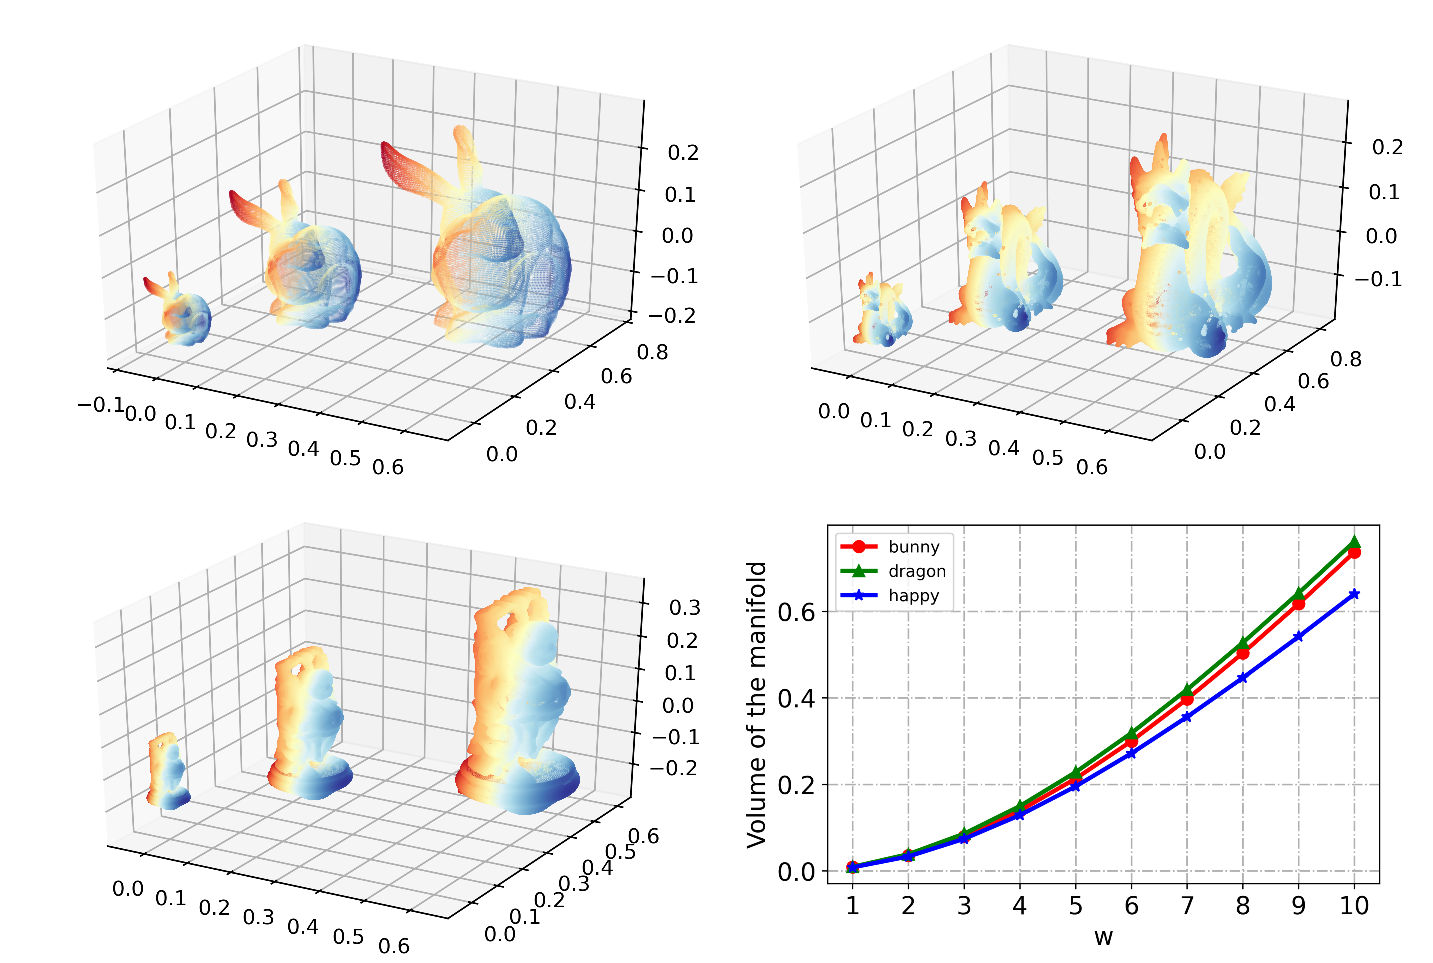
\includegraphics[width=1\columnwidth]{nfig11}
\vskip -0.03in
\caption{Increase three Stanford point cloud manifolds, and calculate their semantic scales.}
\vskip -0.03in
\label{fig11}
\end{center}
\end{figure*}



\section{Experimental Details\label{Experimental Details}}

\subsection{Marginal Effect of Semantic Scale\label{B.1}}

We use the following method to generate new training datasets for classification experiments: assume that the total number of classes in the original dataset is $C$, and $m$ samples are randomly selected from each class to form a sub-dataset with a total number of samples of $C \times m$. The details of the sub-datasets generated based on CIFAR-10, CIFAR-100 and Mini-ImageNet are in Table \ref{table6}.

\begin{table*}[h]
\vskip -0.17in
\renewcommand\arraystretch{2}
\setlength{\tabcolsep}{3.6pt} %修改行距
\caption{The sample-balanced sub-datasets with a total of $31$. Among them, $13$ sub-datasets are from CIFAR-10, $9$ sub-datasets are from CIFAR-100, and the rest are from Mini-ImageNet. The test set remains the original test set. $C$ denotes the total number of classes in the original dataset and $m$ is the number of samples per class in the sub-dataset.}
\label{table6}
%\vskip -0.2in
\begin{center}
\begin{scriptsize}
\begin{tabular}{c|c|p{0.7cm}| ccccccccccccc}
\hline \toprule
Dataset       & $C$  & Number  &  \multicolumn{13}{c}{Sub-datasets} \\
\hline
\multirow{2}{*}{CIFAR-10}  &  \multirow{2}{0.25cm}{10} & \multicolumn{1}{c|}{$m$}  & 50  & 100 &  200 & 300 & 400 & 500 & 600 & 800 & 1,000 & 2,000 & 3,000 & 4,000 & 5,000 \\
  &   & \multicolumn{1}{c|}{$C\! \times\! m$}  & 500  & 1,000 &  2,000 & 3,000 & 4,000 & 5,000 & 6,000 & 8,000 & 10,000 & 20,000 & 30,000 & 40,000 & 50,000 \\
\hline
\multirow{2}{*}{CIFAR-100}  &  \multirow{2}{0.25cm}{\!100} & \multicolumn{1}{c|}{$m$}  & 10  & 20 &  30 & 50 & 100 & 200 & 300 & 400 & 500 & - & - & - & - \\
  &   & \multicolumn{1}{c|}{$C\! \times\! m$}  & 1,000  & 2,000 &  3,000 & 5,000 & 10,000 & 20,000 & 30,000 & 40,000 & 50,000 & - & - & - & - \\
\hline
\multirow{2}{*}{Mini-ImageNet}  &  \multirow{2}{0.25cm}{\!100} & \multicolumn{1}{c|}{$m$}  & 10  & 20 &  30 & 50 & 100 & 200 & 300 & 400 & 500 & - & - & - & - \\
  &   & \multicolumn{1}{c|}{$C\! \times\! m$}  & 1,000  & 2,000 &  3,000 & 5,000 & 10,000 & 20,000 & 30,000 & 40,000 & 50,000 & - & - & - & - \\
\bottomrule \hline
\end{tabular}
\end{scriptsize}
\end{center}
\vskip -0.3in
\end{table*}





\subsection{Quantification of Semantic Scale Imbalance\label{B.2}}

We train ResNet-18 and ResNet-34 on CIFAR-10-LT and CIFAR-10 with an imbalance factor of 200, respectively, and the test set of CIFAR-10-LT is consistent with CIFAR-10. During training, the batch size is fixed to $64$, and the optimizer adopts Adam. The learning rate is initially 0.01 and becomes $0.98$$\times$the previous learning rate after each epoch. We do not employ other additional tricks and data augmentation strategies.



\subsection{Semantic Scale Imbalance on Long-Tailed Data\label{B.3}}

We artificially produce two long-tailed versions of the MNIST dataset, called MNIST-LT-1 and MNIST-LT-2. The number of samples per class is listed in Table \ref{table7}. 

Figure \ref{fig3} shows the class-wise accuracies of ResNet-18 and ResNet-34 trained on CIFAR-10-LT and CIFAR-100-LT with the same training settings as in Appendix \ref{B.2}. Taking CIFAR-10 as an example, labels 1 to 10 correspond to:  \emph{airplane},  \emph{automobile},  \emph{bird},  \emph{cat},  \emph{deer},  \emph{dog},  \emph{frog},  \emph{horse},  \emph{ship},  \emph{truck}. The prediction scores of classification experiments on CIFAR-10-LT and CIFAR-10 find that \emph{cat} (label 4) is most easily confused with \emph{dog} (label 6), as shown by their lowest accuracy on CIFAR-10 (Figure \ref{fig4}). However, the accuracy of \emph{cat} and \emph{dog} on CIFAR-10-LT is higher than that of \emph{deer} (label 5), which is due to the dominant role of semantic scale $S'$ in $S$ for long-tailed data.


\begin{table*}[h]
\vskip -0.1in
\renewcommand\arraystretch{1.5}
\setlength{\tabcolsep}{9pt} %修改行距
\caption{The two long-tailed MNIST datasets resampled from MNIST.}
\label{table7}
\vskip -0.1in
\begin{center}
\begin{tabular}{c|cccccccccc}
\hline \toprule
Dataset       &  \multicolumn{10}{c}{MNIST-LT-1} \\
\hline
Class label & 0 & 1 & 2 & 3 &  4 & 5 & 6 & 7 & 8 & 9 \\ 
Number & 5,923 & 3,590 & 2,940 & 2,518 & 2,256 & 1,972 & 1,700 & 1,300 & 1,100 & 900 \\ \hline
Dataset       &  \multicolumn{10}{c}{MNIST-LT-2} \\
\hline
Class label & 0 & 1 & 2 & 3 &  4 & 5 & 6 & 7 & 8 & 9 \\ 
Number & 5,923 & 3,090 & 2,540 & 1,818 & 1,356 & 972 & 484 & 272 & 122 & 74 \\
\bottomrule \hline
\end{tabular}
\end{center}
\vskip -0.1in
\end{table*}



\subsection{Semantic Scale Imbalance for More Datasets\label{B.4}}


We have demonstrated the semantic scale imbalance on MNIST, MNIST-LT, CIFAR-10, CIFAR-10-LT, CIFAR-100 and CIFAR-100-LT in Section 3.4. Figure \ref{fig5} additionally shows the degree of semantic scale imbalance on CUB-2011, Cars196, and Mini-ImageNet, indicating that the semantic scale imbalance is indeed prevalent in all kinds of datasets.



\begin{figure*}[h] % 纵向8行,图片靠右,宽度12.5em
\begin{center}
\vskip -0.02in
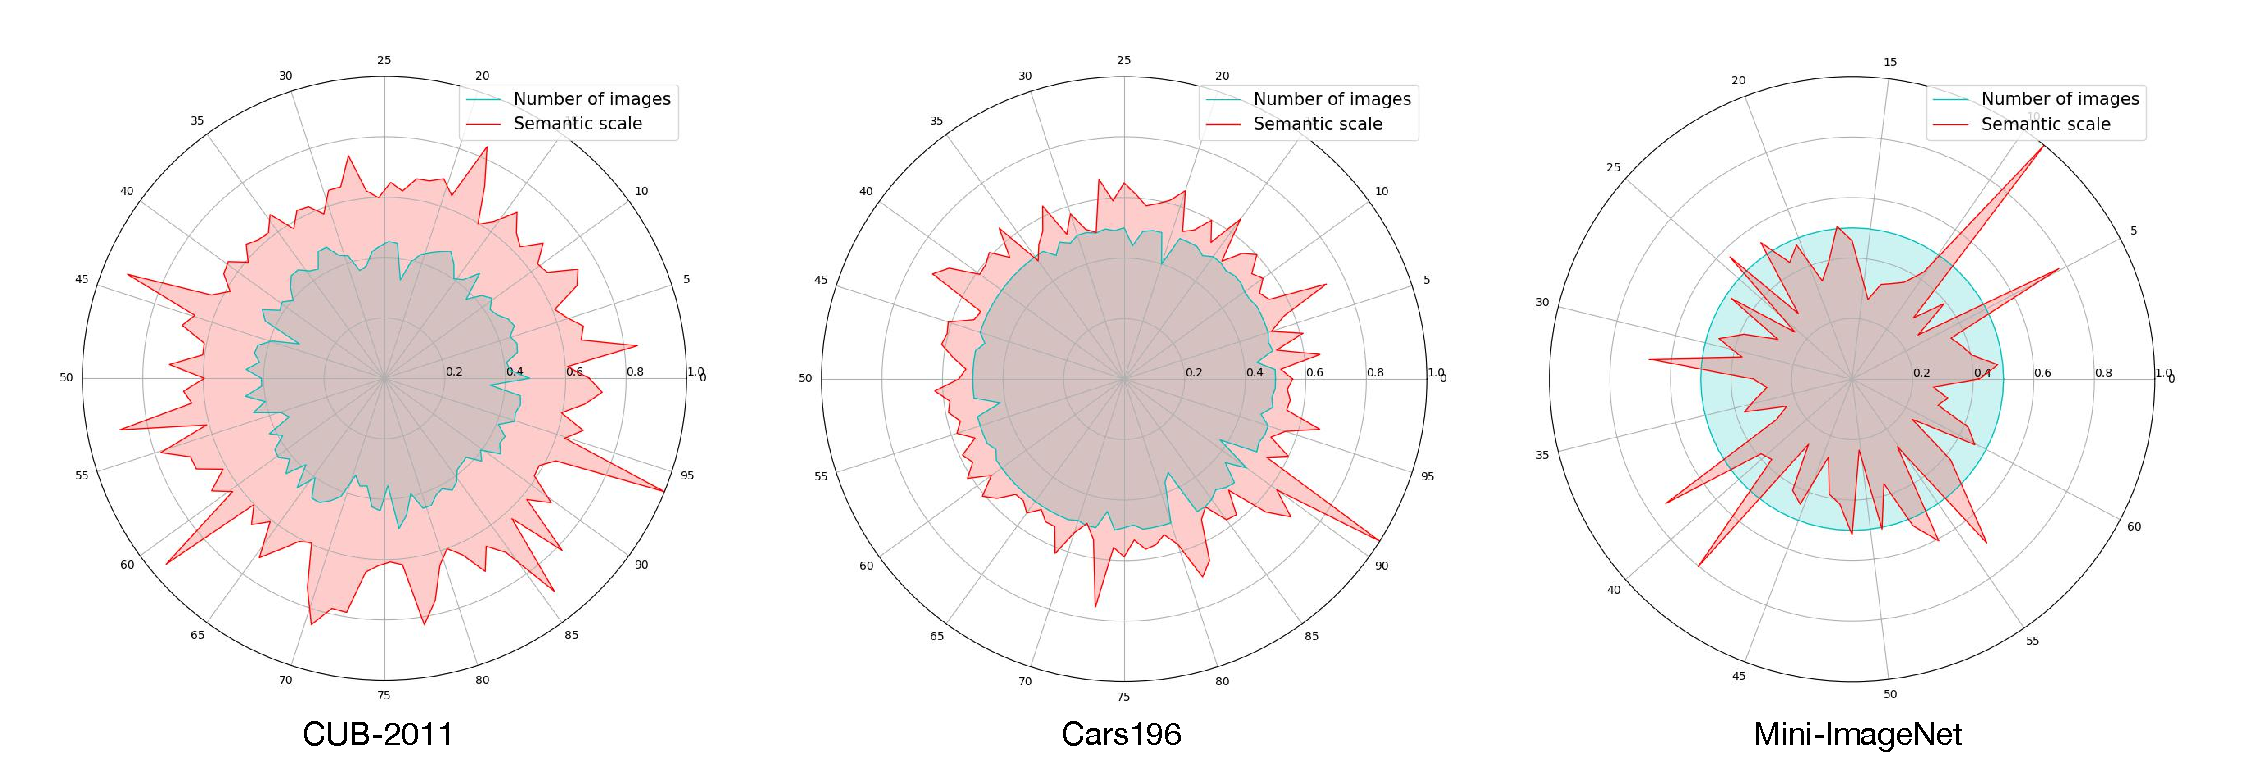
\includegraphics[width=1\columnwidth]{figure5}
\vskip -0.05in
\caption{Semantic scale and number of samples per class. Different angles of the radar plot represent different classes, and the number of samples in the largest class is normalized to 0.5 for ease of observation.}
\vskip -0.03in
\label{fig5}
\end{center}
\end{figure*}




\subsection{Experimental Settings for Section 5.3 and More Experiments\label{B.5}}


\subsubsection{Experimental Settings for Section 5.3\label{B.5.1}}

\textbf{Backbone Network and Experimental Parameters}. Since we improve on the classical loss in the field of deep metric learning, we abide by the widely adopted backbone network, experimental parameters, and the division of datasets in this field. The BN-Inception \cite{paper38,paper78} pre-trained on ImageNet is adopted as the backbone network, and the training set is augmented by using random horizontal flipping and random cropping. All images are cropped to 224$\times$224 as the input of the network. The output of the network after global average pooling is fed into a single fully connected layer to obtain 64- or 512-dimensional feature embeddings, and then all embeddings are clustered by K-means. The model is optimized by Adam with the batch size as 32 and the number of epochs as 50. We evaluate the performance of the learned embeddings with Recall@K and Normalized Mutual Information (NMI). The remaining experimental parameters used in the training are consistent with those reported in NormSoftmax and SoftTriple \cite{paper82}.



\textbf{Dataset Introduction (CUB-2011, Cars196 and CIFAR-100-LT)}. The CUB-2011 dataset has 5,864 images in the first 100 classes for training and 5,924 images in the second 100 classes for testing. The Cars196 dataset consists of 196 classes totaling 16,185 images, with the first 98 classes for training and the remaining classes for testing. The CIFAR-100 has 100 classes, each containing 600 images. We create three long-tailed CIFAR-100 with the first 60 classes for training (See Figure \ref{fig6}a) and test on the remaining classes \cite{paper82}. 


\begin{figure*}[h] % 纵向8行,图片靠右,宽度12.5em
\begin{center}
%\vskip -0.05in
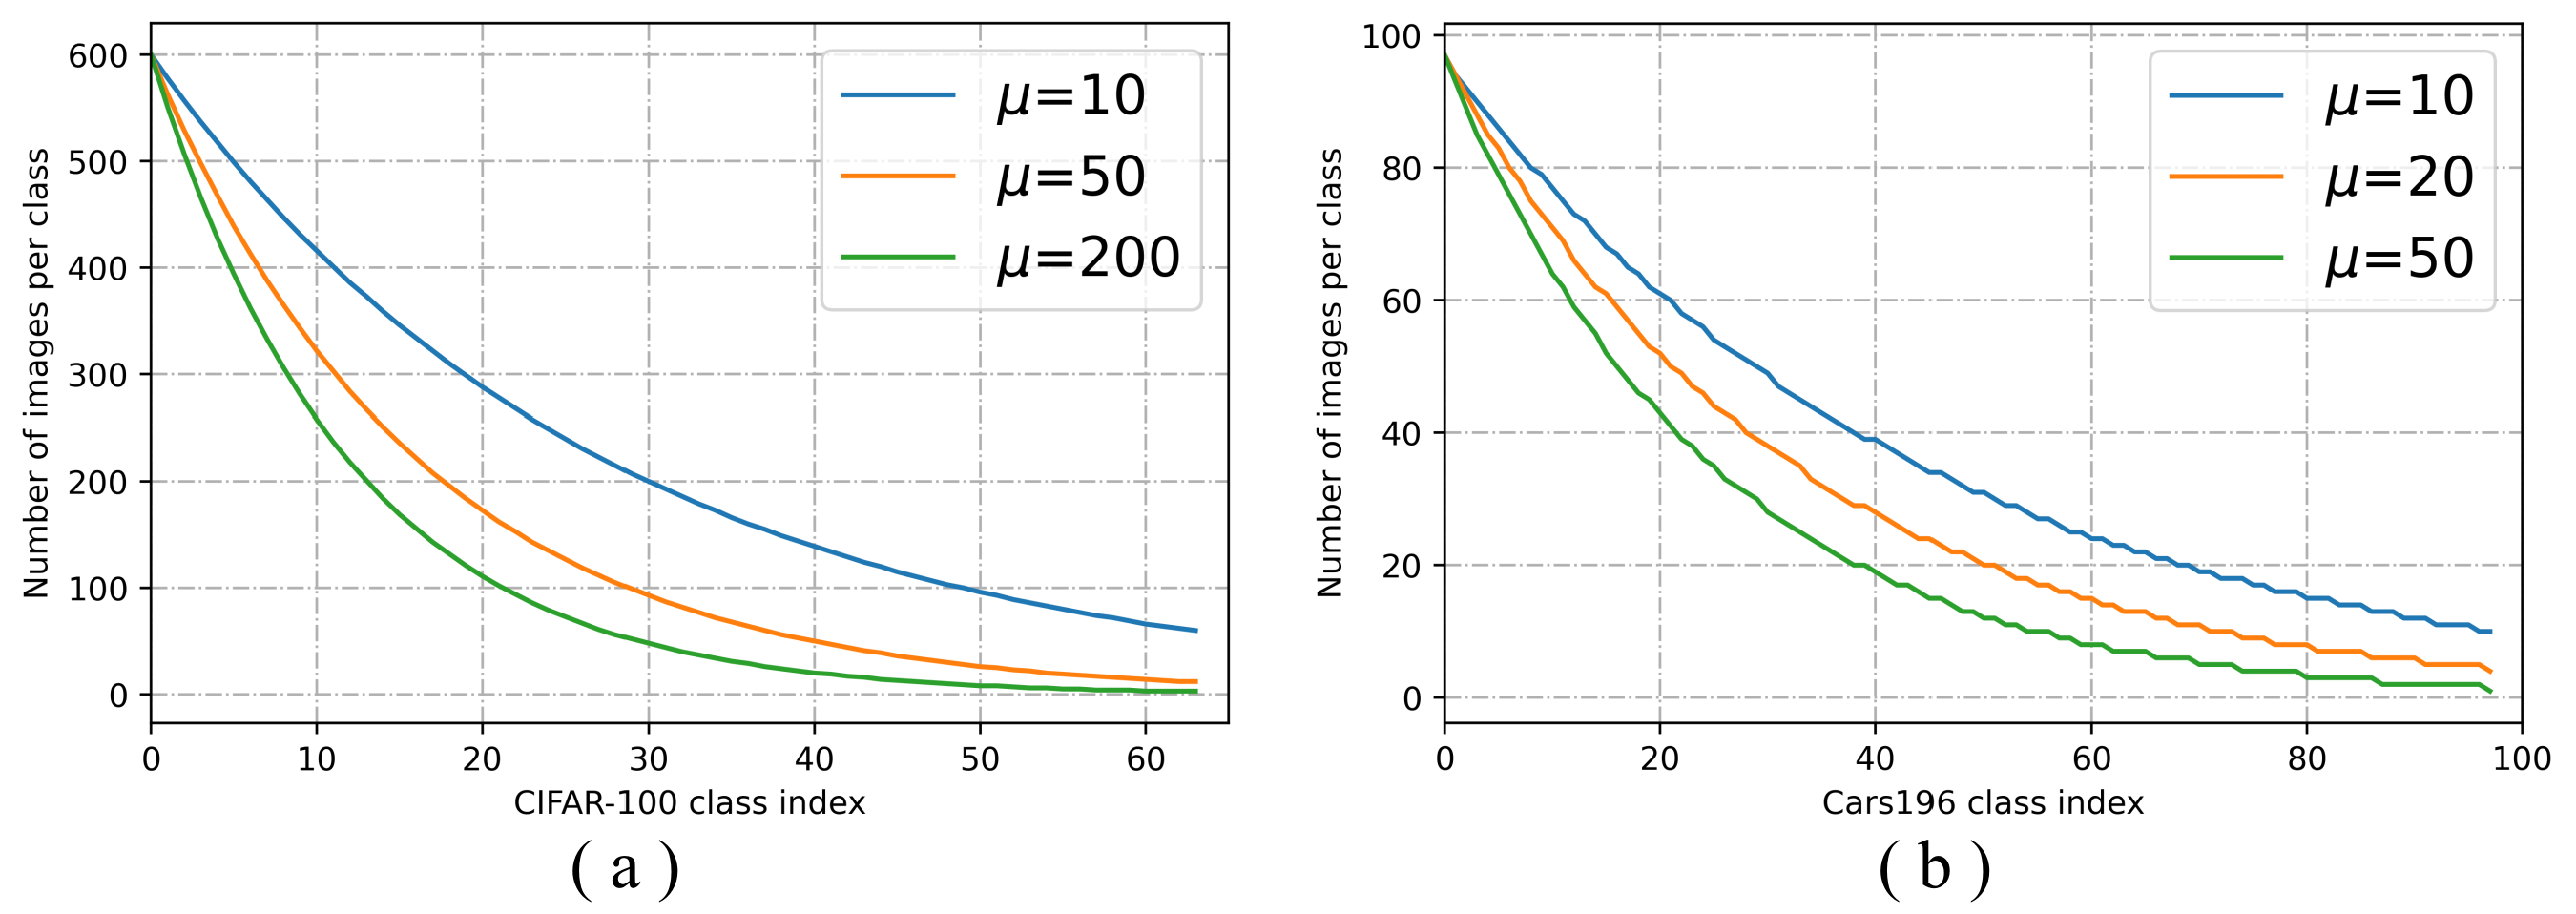
\includegraphics[width=0.95\columnwidth]{fig6}
\vskip -0.05in
\caption{Long-tailed CIFAR100 and Cars196 with different imbalance factors. We use the exponential function ${n_i} = N\!{\mu ^{{i \mathord{/
 {\vphantom {i {( {1 - M} )}}} 
 \kern-\nulldelimiterspace} {( {1 - M} )}}}}$ to yield the number of training samples for each class, where $i$ is the class index (0-indexed), $N$ is the number of training samples in the largest class, $\mu$ is the imbalance factor, and $M$ is the total number of classes.}
\vskip -0.2in
\label{fig6}
\end{center}
\end{figure*}


\subsubsection{More Experiments\label{B.5.2}}

The long-tailed Cars196 is created using the first 98 classes for training (See Figure \ref{fig6}b) and the test set is the remaining classes. Both Mini-ImageNet and CIFAR-100 datasets contain 100 classes, each containing 600 samples. For the Mini-ImageNet dataset, the first 64 classes are the training set and the last 36 classes are the test set, and for the CIFAR-100 dataset, the first 60 classes are the training set and the remaining classes are the test set. Note that the experiments on CIFAR-100 in this section are different from the classification experiments on CIFAR-100 in Sec \ref{5.3}. The purpose of this experiments is to complement the effectiveness of our proposed method on both long-tailed and sample-balanced datasets for the field of deep metric learning.


\begin{table}[h]
\vskip -0.1in
\caption{Comparison on long-tailed Cars196.}
\vskip 0.05in
\label{table8}
\centering  
%\resizebox{.95\columnwidth}{!}{
\renewcommand\arraystretch{1.4}
\setlength{\tabcolsep}{9.5pt} %修改行距
\begin{tabular}{ c|l |ccc | ccc  |ccc }
\hline \toprule 
\multicolumn{2}{c|}{Dataset}    & \multicolumn{9}{c}{Long-tailed Cars196}    \\ \hline
\multicolumn{2}{c|}{Imbalance factor}   & \multicolumn{3}{c|}{10}  &  \multicolumn{3}{c|}{20}  & \multicolumn{3}{c}{50} \\ \hline
\multicolumn{2}{c|}{Metric}     & R@1     & R@2    & NMI     & R@1     & R@2     & NMI    & R@1     & R@2     & NMI\\  \hline
\multirow{6}{12pt}[-5pt]{dim\\64}  & NormSoftmax      &66.4    & 76.9   & 58.9   & 63.1   & 74.2   & 54.9  & 59.5   & 71.1   & 52.9\\
& CB-NSM         & 68.9   & 78.0   & 60.1   & 64.9   & 75.2   & 56.1   & 61.7   & 72.5  &53.3  \\  
& \textbf{DSB-NSM}      & \textbf{69.5}   & \textbf{78.6}    & \textbf{60.7}   & \textbf{65.4}   & \textbf{75.7}   & \textbf{56.6}   & \textbf{62.3}   & \textbf{73.0}   &\textbf{54.1} \\  \cline{2-11}
&SoftTriple                      &70.2    & 80.5  & 61.4   & 64.7   & 75.8   & 57.5  & 62.9   & 74.1  & 55.2\\
&CB-ST                     & 71.9   & 81.3   & 62.9   & 66.5   & 76.9   & 58.6   & 64.8   &75.4   &56.0 \\
&\textbf{DSB-ST}                  & \textbf{72.3}   & \textbf{81.8}   & \textbf{63.4}   & \textbf{66.8}   & \textbf{77.5}   & \textbf{59.7}   & \textbf{65.4}   & \textbf{75.3}   &\textbf{56.6} \\ \bottomrule  \hline
 \end{tabular}
\vskip -0.02in
 \end{table} 


Table \ref{table8} shows the performance comparison of DSB-NSM and DSB-ST on the long-tailed Car196. When the imbalance factor is 10, DSB-NSM outperforms NSM (NormSoftmax) by \textbf{3.1\%} on R@1 and DSB-ST outperforms ST (SoftTriple) by \textbf{2.1\%}. When the imbalance factor is 50, DSB-NSM and DSB-ST improve \textbf{2.8\%} and \textbf{2.5\%}, respectively, on R@1 compared to the original method. In addition, DSB loss performs better than CB loss on all metrics.

Table \ref{table9} shows that compared with the original losses, DSB-NSM and DSB-ST are able to consistently improve R@1 by \textbf{1.3\%} on average and NMI by \textbf{1-2\%} for both sample-balanced datasets, with all other metrics outperforming the original. The results in Tables 8 and 9 further confirm that our proposed dynamic semantic-scale-balanced learning is applicable to long-tailed and sample-balanced datasets in the field of deep metric learning, and has broad application prospects.


\begin{table}[H]
\vskip -0.05in
\renewcommand\arraystretch{1.2}
\setlength{\tabcolsep}{6.3pt} %修改行距
\caption{Comparison on Mini-ImageNet and CIFAR-100.}
\vskip 0.05in
\label{table9}
\centering  
%\begin{scriptsize}
%\resizebox{.95\columnwidth}{!}{
\begin{tabular}{l|lll| lll}
\hline \toprule 
\multicolumn{1}{c|}{Dataset}    & \multicolumn{3}{c}{Mini-ImageNet}  & \multicolumn{3}{|c}{CIFAR-100}  \\ \midrule
\multicolumn{1}{c|}{Metric}    & R@1   & R@2   & NMI  & R@1   & R@2   & NMI  \\  \toprule
NormSoftmax &85.7 & 91.2  & 74.1  & 60.1 & 71.5 & 49.4\\
\textbf{DSB-NSM}  & \textbf{87.1}(\textcolor[RGB]{0,201,87}{\textbf{+1.4}}) & \textbf{92.0}(\textcolor[RGB]{0,201,87}{\textbf{+0.8}})  & \textbf{75.5}(\textcolor[RGB]{0,201,87}{\textbf{+1.4}}) & \textbf{61.4}(\textcolor[RGB]{0,201,87}{\textbf{+1.3}}) & \textbf{72.2}(\textcolor[RGB]{0,201,87}{\textbf{+0.7}})  & \textbf{50.6}(\textcolor[RGB]{0,201,87}{\textbf{+1.2}}) \\  \midrule 
SoftTriple & 86.9 & 92.0  & 77.3 &62.1 & 73.3 & 52.0  \\ 
\textbf{DSB-ST}  & \textbf{88.0}(\textcolor[RGB]{0,201,87}{\textbf{+1.1}}) & \textbf{92.8}(\textcolor[RGB]{0,201,87}{\textbf{+0.8}})  & \textbf{78.8}(\textcolor[RGB]{0,201,87}{\textbf{+1.5}}) & \textbf{63.5}(\textcolor[RGB]{0,201,87}{\textbf{+1.4}}) & \textbf{73.9}(\textcolor[RGB]{0,201,87}{\textbf{+0.6}})  & \textbf{53.0}(\textcolor[RGB]{0,201,87}{\textbf{+1.0}}).  \\ \bottomrule \hline
 \end{tabular}
 %\end{scriptsize}
\vskip -0.1in
\end{table}



%%%%%%%%%%%%%%%%%%%%%%%%%%%%
%%.             OIA                               %%%%%%%%%%
%%%%%%%%%%%%%%%%%%%%%%%%%%%%
\subsection{Results on the fundus datasets OIA-ODIR and OIA-ODIR-B\label{B.6}}

\subsubsection{Dataset Introduction}
The OIA-ODIR dataset \cite {paper109} was made public in 2019, and it contains a total of 10,000 fundus images in 8 classes. As shown in Figure \ref{fig30}, the eight classes are: Normal(N), hypertensive retinopathy(D), glaucoma(G), cataract(C), agerelated macular degeneration(A) , hypertension complication (H), pathologic myopia (M), other disease / abnormality(O). Considering that O usually appears together with other diseases, to reduce ambiguity, we adopt the data splitting scheme of \cite {paper110}, using only the data of the first 7 classes, and the number of training samples and test samples for each class is shown in Figure \ref{fig12}.

\begin{figure*}[h]
\begin{center}
%\vskip -0.3in
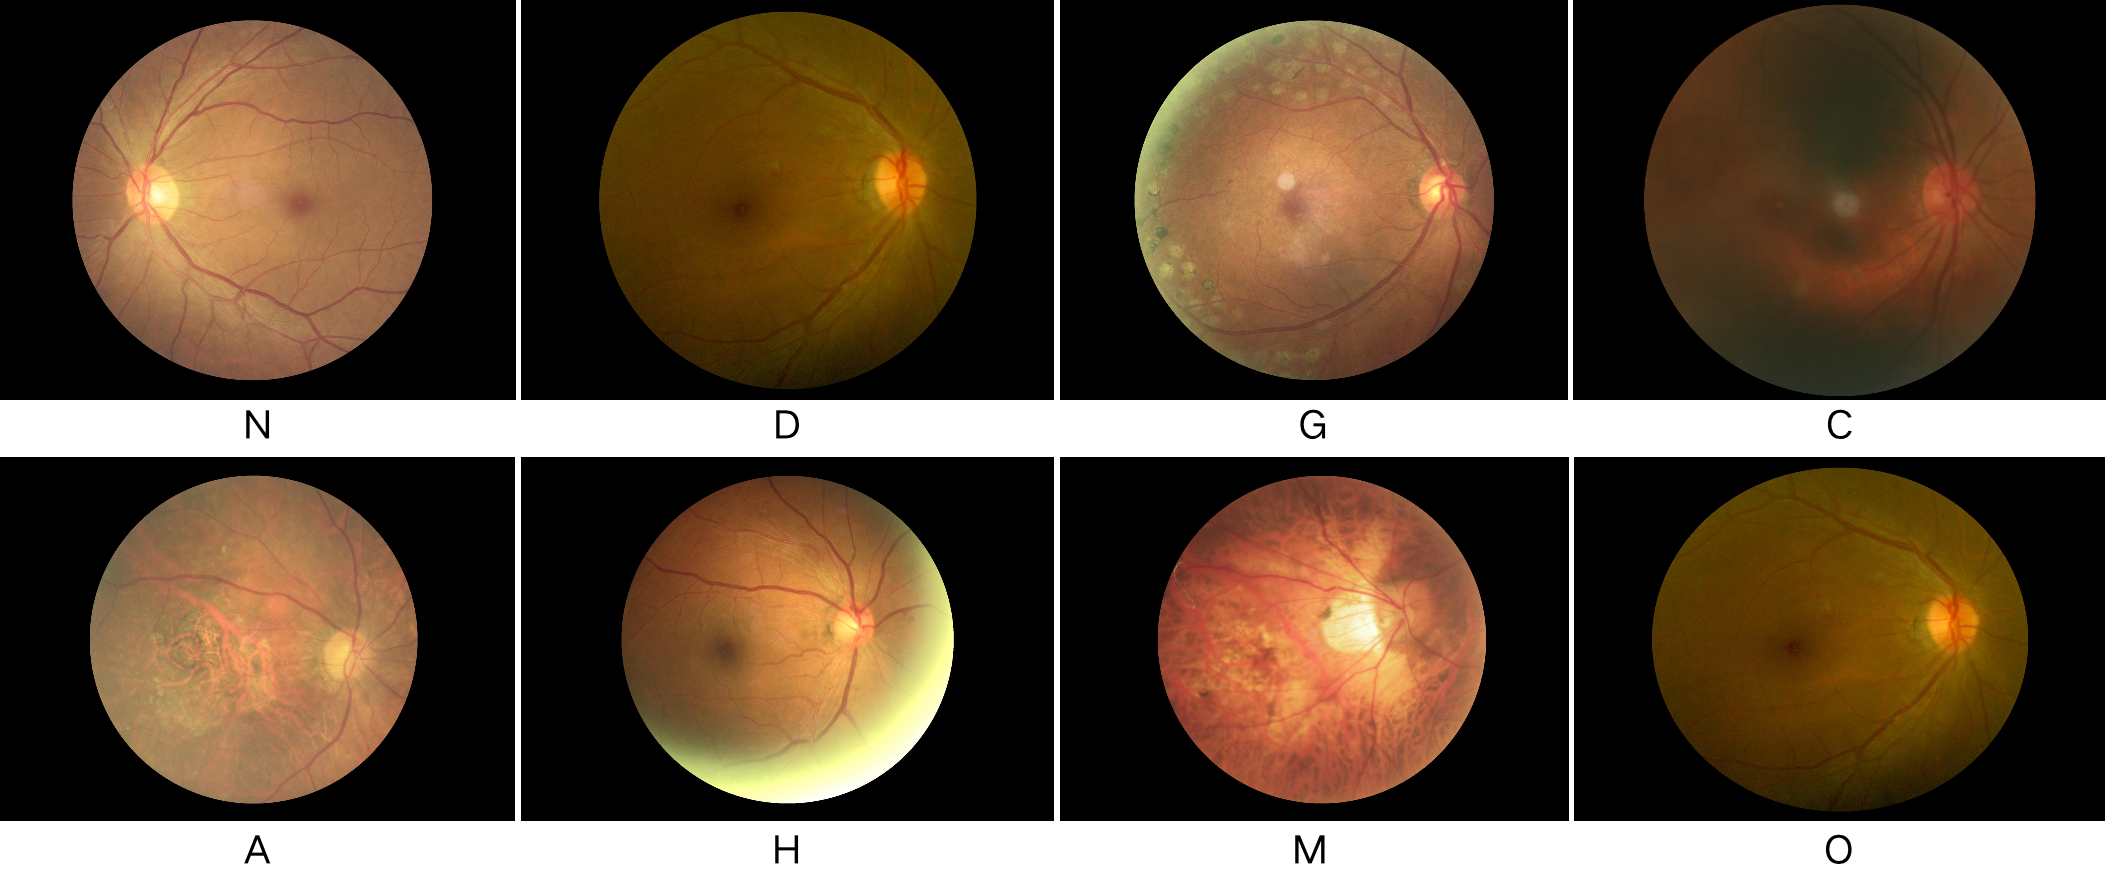
\includegraphics[width=1\columnwidth]{fig30}
\vskip -0.07in
\caption{Eight fundus images in the OIA-ODIR dataset.}
\label{fig30}
\end{center}
\vskip -0.1in
\end{figure*}


The OIA-ODIR dataset suffers from an unbalanced number of samples. To fully validate our method, we produced a balanced version of the OIA-ODIR dataset, OIA-ODIR-B, by using the class with the least number of samples as the benchmark. As shown in Figure \ref{fig12}, each class of OIA-ODIR-B contains 103 training samples and 46 test samples.

In addition to the number of samples, we plot the degree of semantic scale imbalance for the training sets of OIA-ODIR and OIA-ODIR-BS in Figure \ref{fig12}.

\begin{figure*}[h]
\begin{center}
%\vskip -0.3in
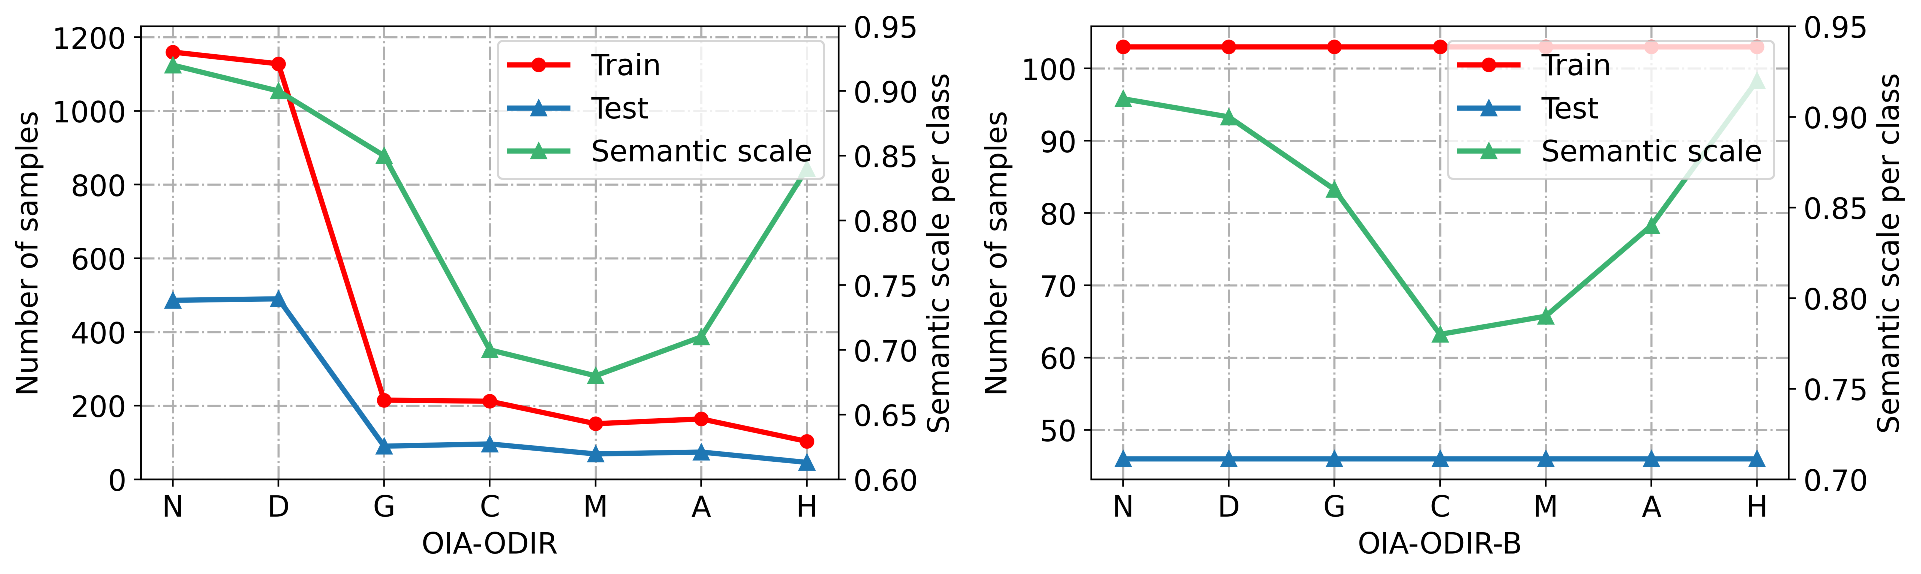
\includegraphics[width=1\columnwidth]{nfig12}
\vskip -0.1in
\caption{The number of training and test samples for each category and the degree of semantic scale imbalance in OIA-ODIR and OIA-ODIR-B.}
\label{fig12}
\end{center}
\vskip -0.05in
\end{figure*}

\subsubsection{Backbone Network and Experimental Parameters} 
We used ResNet-50, pre-trained on ImageNet, as the backbone network. An adam optimizer with a learning rate of 0.1 (linear decay), a momentum of 0.9, and a weight decay factor of 0.005 was adopted to train all networks. In keeping with \cite {paper110}, average precision (AP) was used as the performance metric of the model.


\subsubsection{Results on OIA-ODIR}
We improved the advanced class rebalancing method (BS \cite {paper105}, Focal loss \cite {paper14}, LDAM \cite {paper104}) and the classification results are plotted in Figure \ref{fig13}. The experimental findings are summarized as follows.

\begin{figure*}[h]
\begin{center}
%\vskip -0.3in
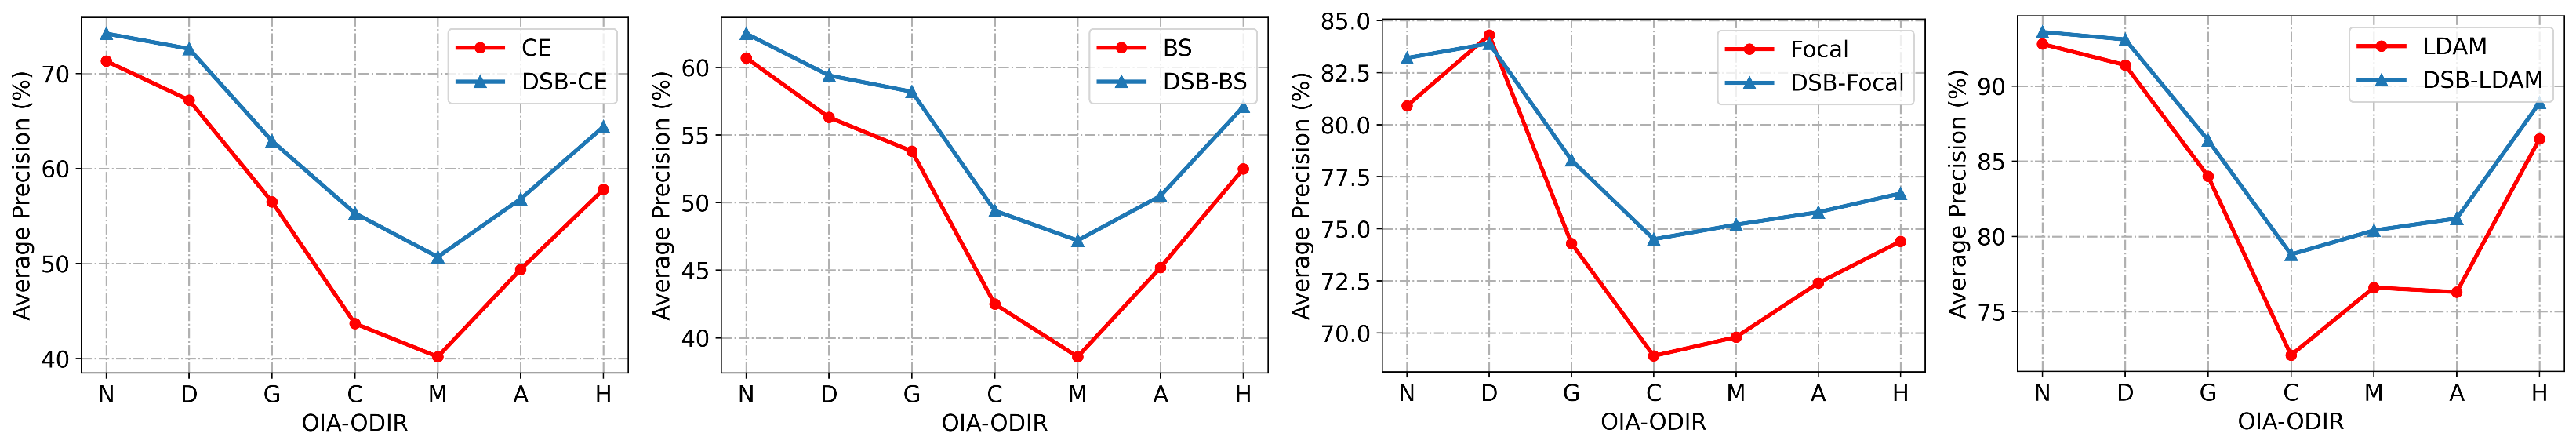
\includegraphics[width=1\columnwidth]{nfig13}
\vskip -0.05in
\caption{The enhancement effect of our method for CE, BS, Focal, and LDAM on the OIA-ODIR.}
\label{fig13}
\end{center}
\vskip -0.15in
\end{figure*}

\begin{itemize}
    \item Although the sample from class H is the smallest, all methods outperform on class H than on class C, class M, and class A. This again shows that the number of samples is not the best measure of class imbalance.
    \item Methods based on sample numbers usually result in larger boosts for the classes with the smallest sample numbers and thus fail to give more attention to class C, class M, and class A. Our method has the most significant boosts for these three classes, indicating that semantic scale imbalance can more accurately reflect the difficulty of the classes.
\end{itemize}


\subsubsection{Results on OIA-ODIR-B} 
Since the class rebalancing method based on the number of samples cannot be applied to the dataset with a balanced number of samples, we additionally adopted VGG-16, ResNet-18 and SE-ResNet-50 as the backbone network to test the effect of DSB-CE on CE enhancement, and the experimental results are shown in Figure \ref{fig14}. The experimental findings are summarized as follows.

\begin{figure*}[h]
\begin{center}
%\vskip -0.3in
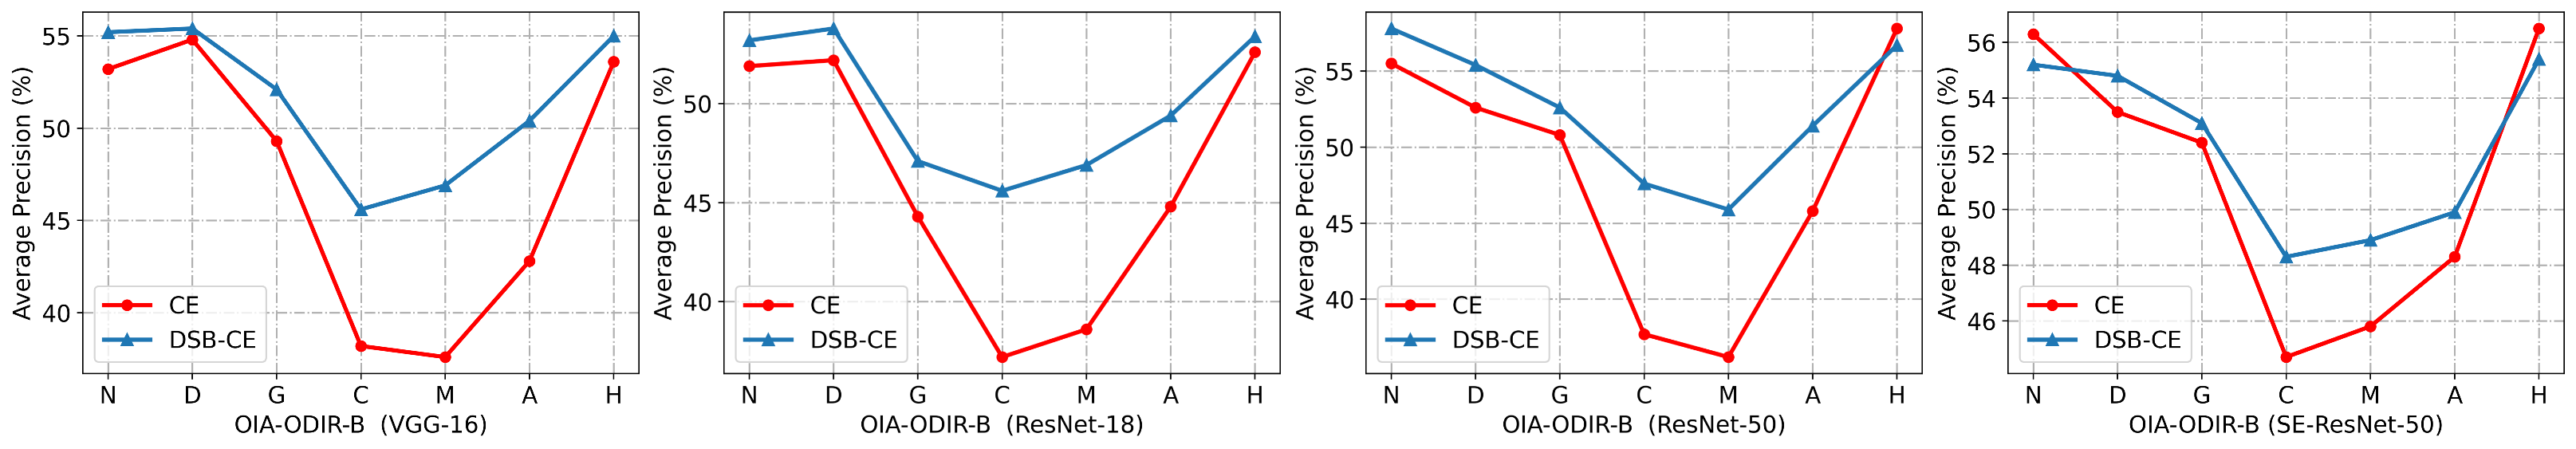
\includegraphics[width=1\columnwidth]{fig14}
\vskip -0.05in
\caption{Performance gains from our approach for multiple backbone networks on OIA-ODIR.}
\label{fig14}
\end{center}
\vskip -0.15in
\end{figure*}

\begin{itemize}
    \item With a balanced number of samples, the model still performs poorly on class C, class M and class A. Figure \ref{fig12} shows that the semantic scales of these three classes are significantly smaller than the other classes.
    \item Our approach results in significant performance gains for all models on class C, class M, and class A, and promotes more balanced model performance on all classes, which is important in medical AI.
\end{itemize}

\textbf{Experiment Summary.} We validated the effectiveness of semantic-scale-balanced learning both on a dataset of fundus images with balanced sample numbers and on a long-tailed dataset of fundus images. Experimental results show that semantic scale imbalance exists in medical image datasets and significantly limits the performance of deep neural networks, so it is necessary to introduce semantic-scale-balanced learning in medical image classification.

%%%%%%%%%%%%%%%%%%%%%%%%%%%%
%%.             END-OIA                      %%%%%%%%%%
%%%%%%%%%%%%%%%%%%%%%%%%%%%%



%%%%%%%%%%%%%%%%%%%%%%%%%%%%
%%.             Remote sensing              %%%%%%%%%
%%%%%%%%%%%%%%%%%%%%%%%%%%%%
\subsection{Remote sensing image scene classification\label{B.7}}

In this section, we validate the effectiveness of semantic-scale-balanced learning in a sample-balanced remote sensing image classification task, which demonstrates the necessity of introducing semantic scale imbalance into the field of remote sensing image recognition.

\subsubsection{Dataset Introduction}

\begin{itemize}
\item \textbf{RSSCN7} dataset contains $2,800$ remote sensing images which are classified into $7$ typical scene categories: grassland, forest, farmland, parking lot, residential region, industrial region, and river and lake. Figure \ref{fig31} shows the images of the seven scenarios. Following the official split, the number of images for training and testing is $50$\% of the total number each.

\item \textbf{NWPU-RESISC45} dataset contains a total of $31,500$ images with pixel size of $256\times256$, covering $45$ scene classes with $700$ images in each class. This dataset has large intra-class variability and inter-class similarity due to the large differences in image spatial resolution, untitled pose, and illumination. Following the official split, $20$\% of the images are used for training and $80$\% for testing.
\end{itemize}

\begin{figure*}[h]
\begin{center}
%\vskip -0.3in
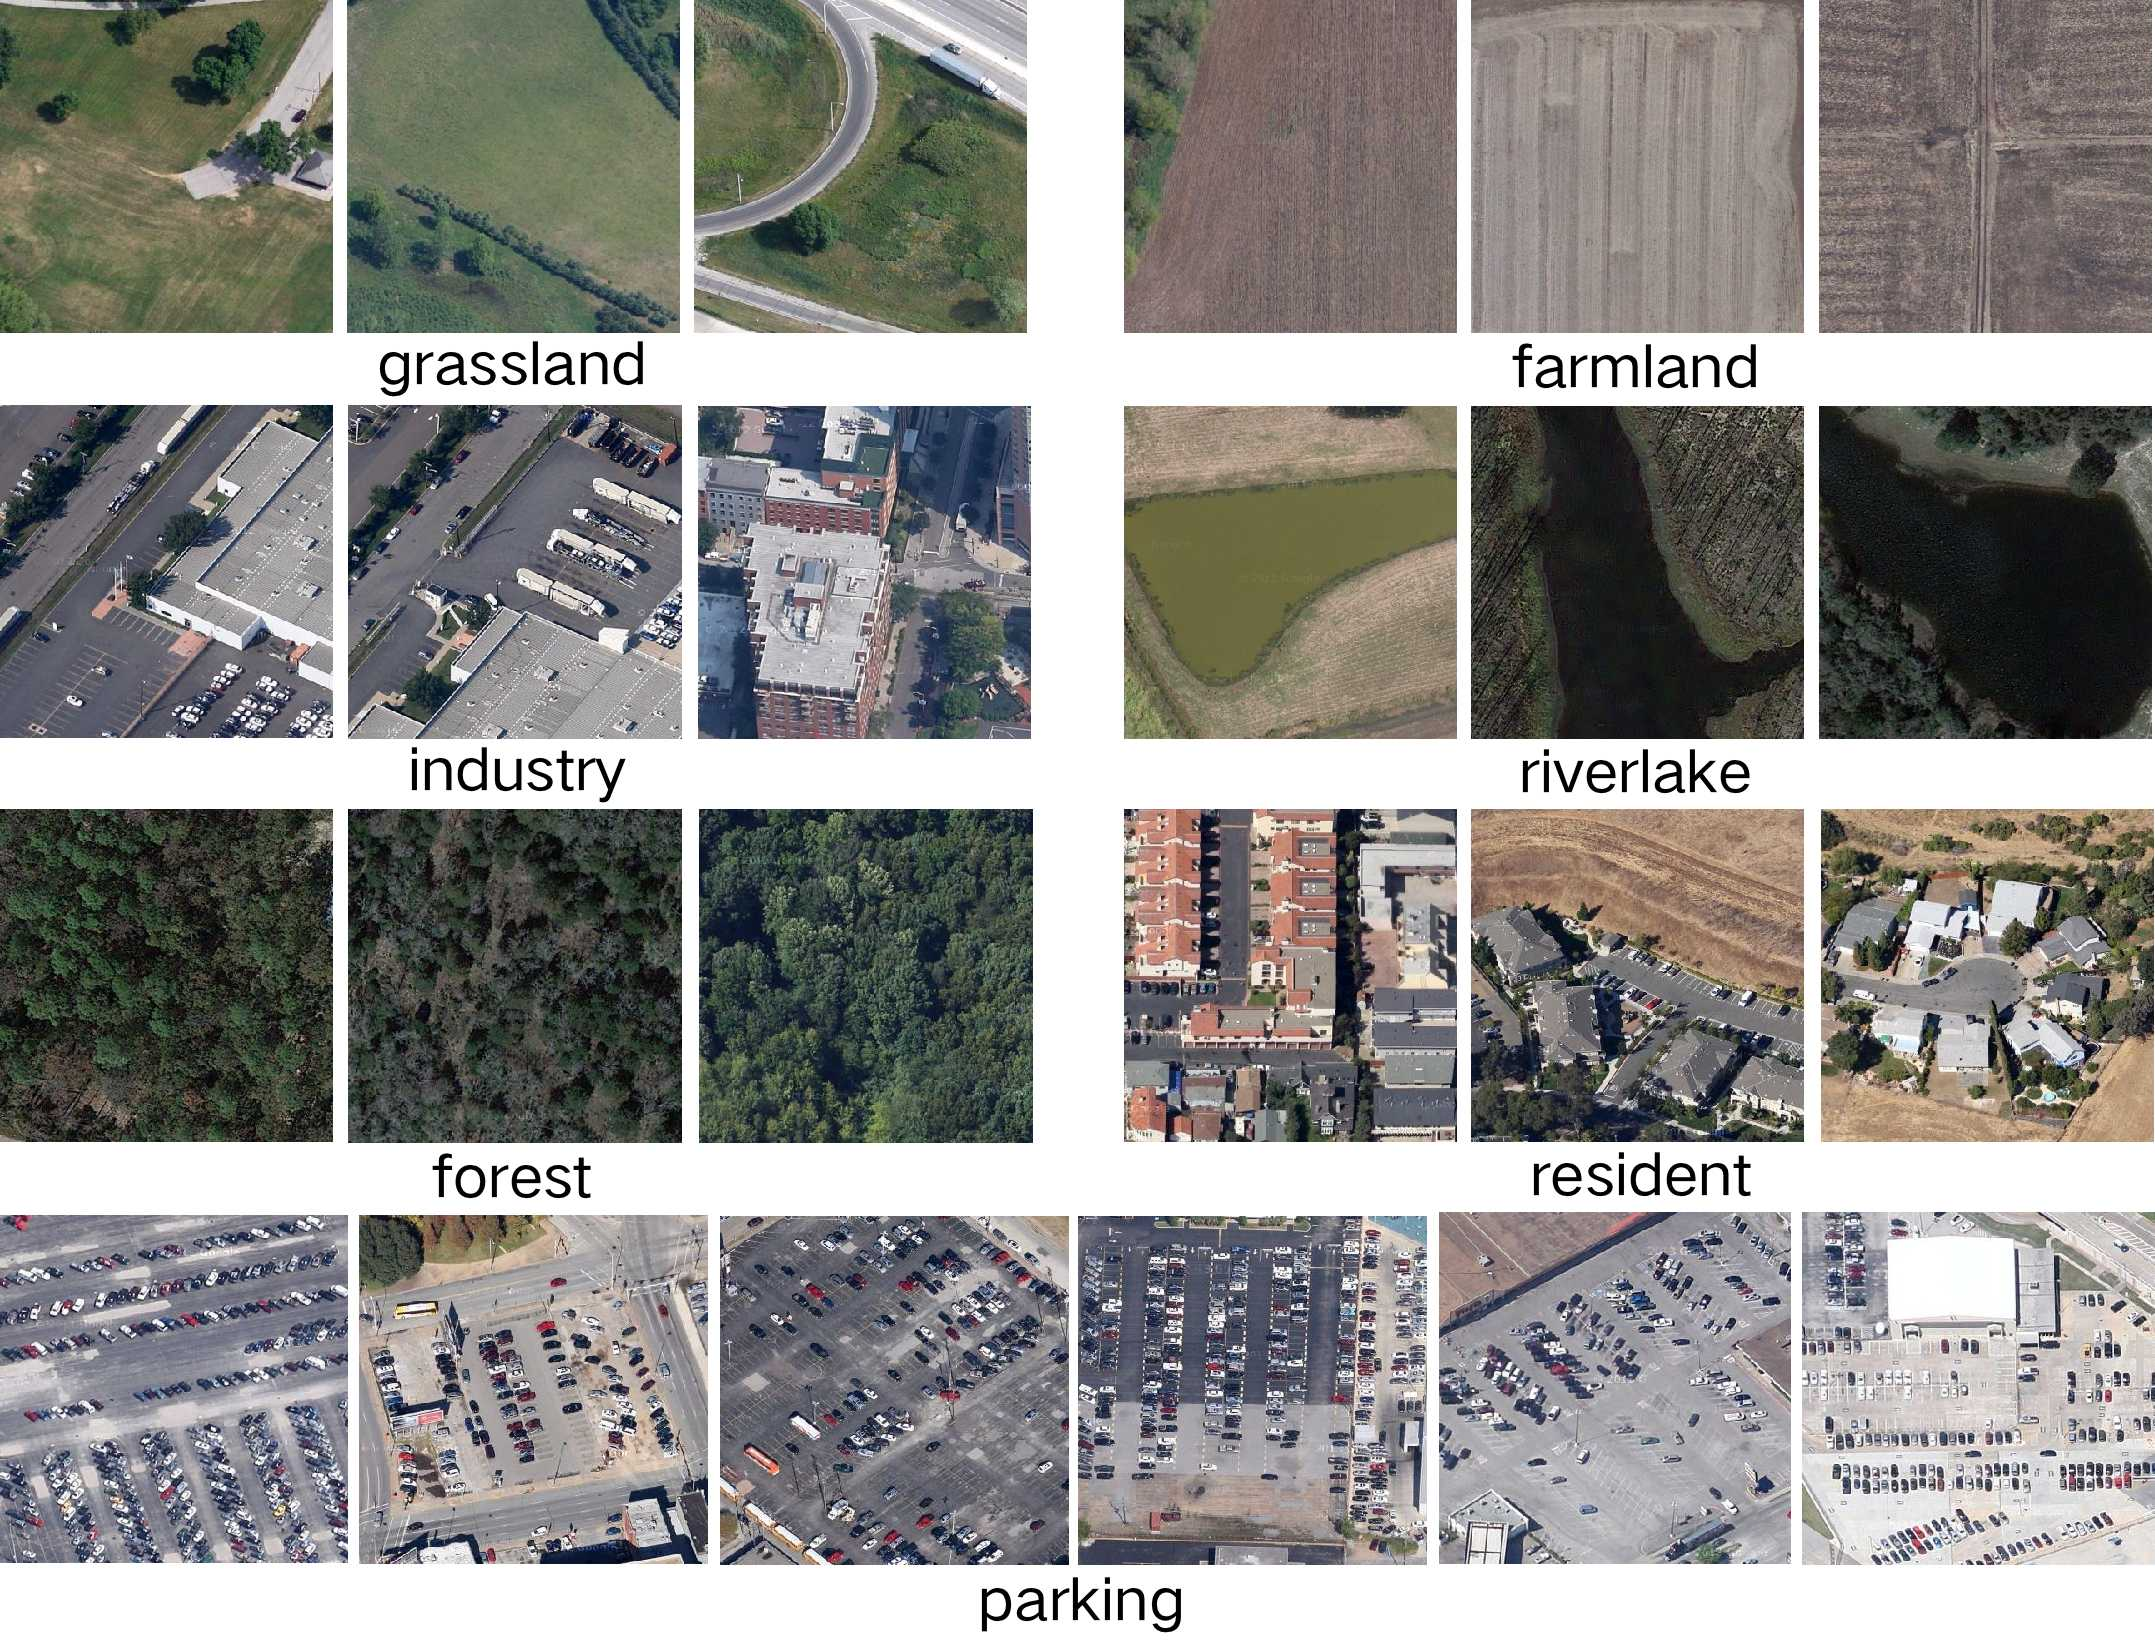
\includegraphics[width=0.9\columnwidth]{fig31}
\vskip -0.12in
\caption{The seven scenarios are included in the RSSCN7 dataset.}
\label{fig31}
\end{center}
\vskip -0.3in
\end{figure*}

\subsubsection{Backbone Network and Experimental Parameters}
We select VGG-16, GoogLeNet, and ResNet-34 as the backbone networks. The Adam optimizer (default parameter) is adopted to update the model until convergence, and the learning rate decays $10$ times every $50$ epochs. In addition, the batch size is set to $100$ and no data augmentation is used throughout the training process.


\subsubsection{Results on RSSCN7} 

We trained all backbone networks with dynamic semantic-scale-balanced learning. The experimental results are shown in Figure \ref{fig32}. It can be found that our method improves the performance of all models. When our method is not employed, all backbone networks are significantly weaker in recognizing industrial regions than other scenes. Our method makes the recognition ability of the model for different scenes more balanced, thus improving the overall performance of the model. 

Specifically, dynamic semantic-scale-balanced learning improves VGG-16's recognition accuracy for industrial regions and parking lots by $4$\% and $3$\%, respectively, significantly reducing the bias of the model. Dynamic semantic-scale-balanced learning also performs well on GoogLeNet and ResNet-34, where it improves the overall accuracy of GoogLe and ResNet by $1$\% and $0.6$\%, respectively.

\begin{figure*}[t]
\begin{center}
%\vskip -0.1in
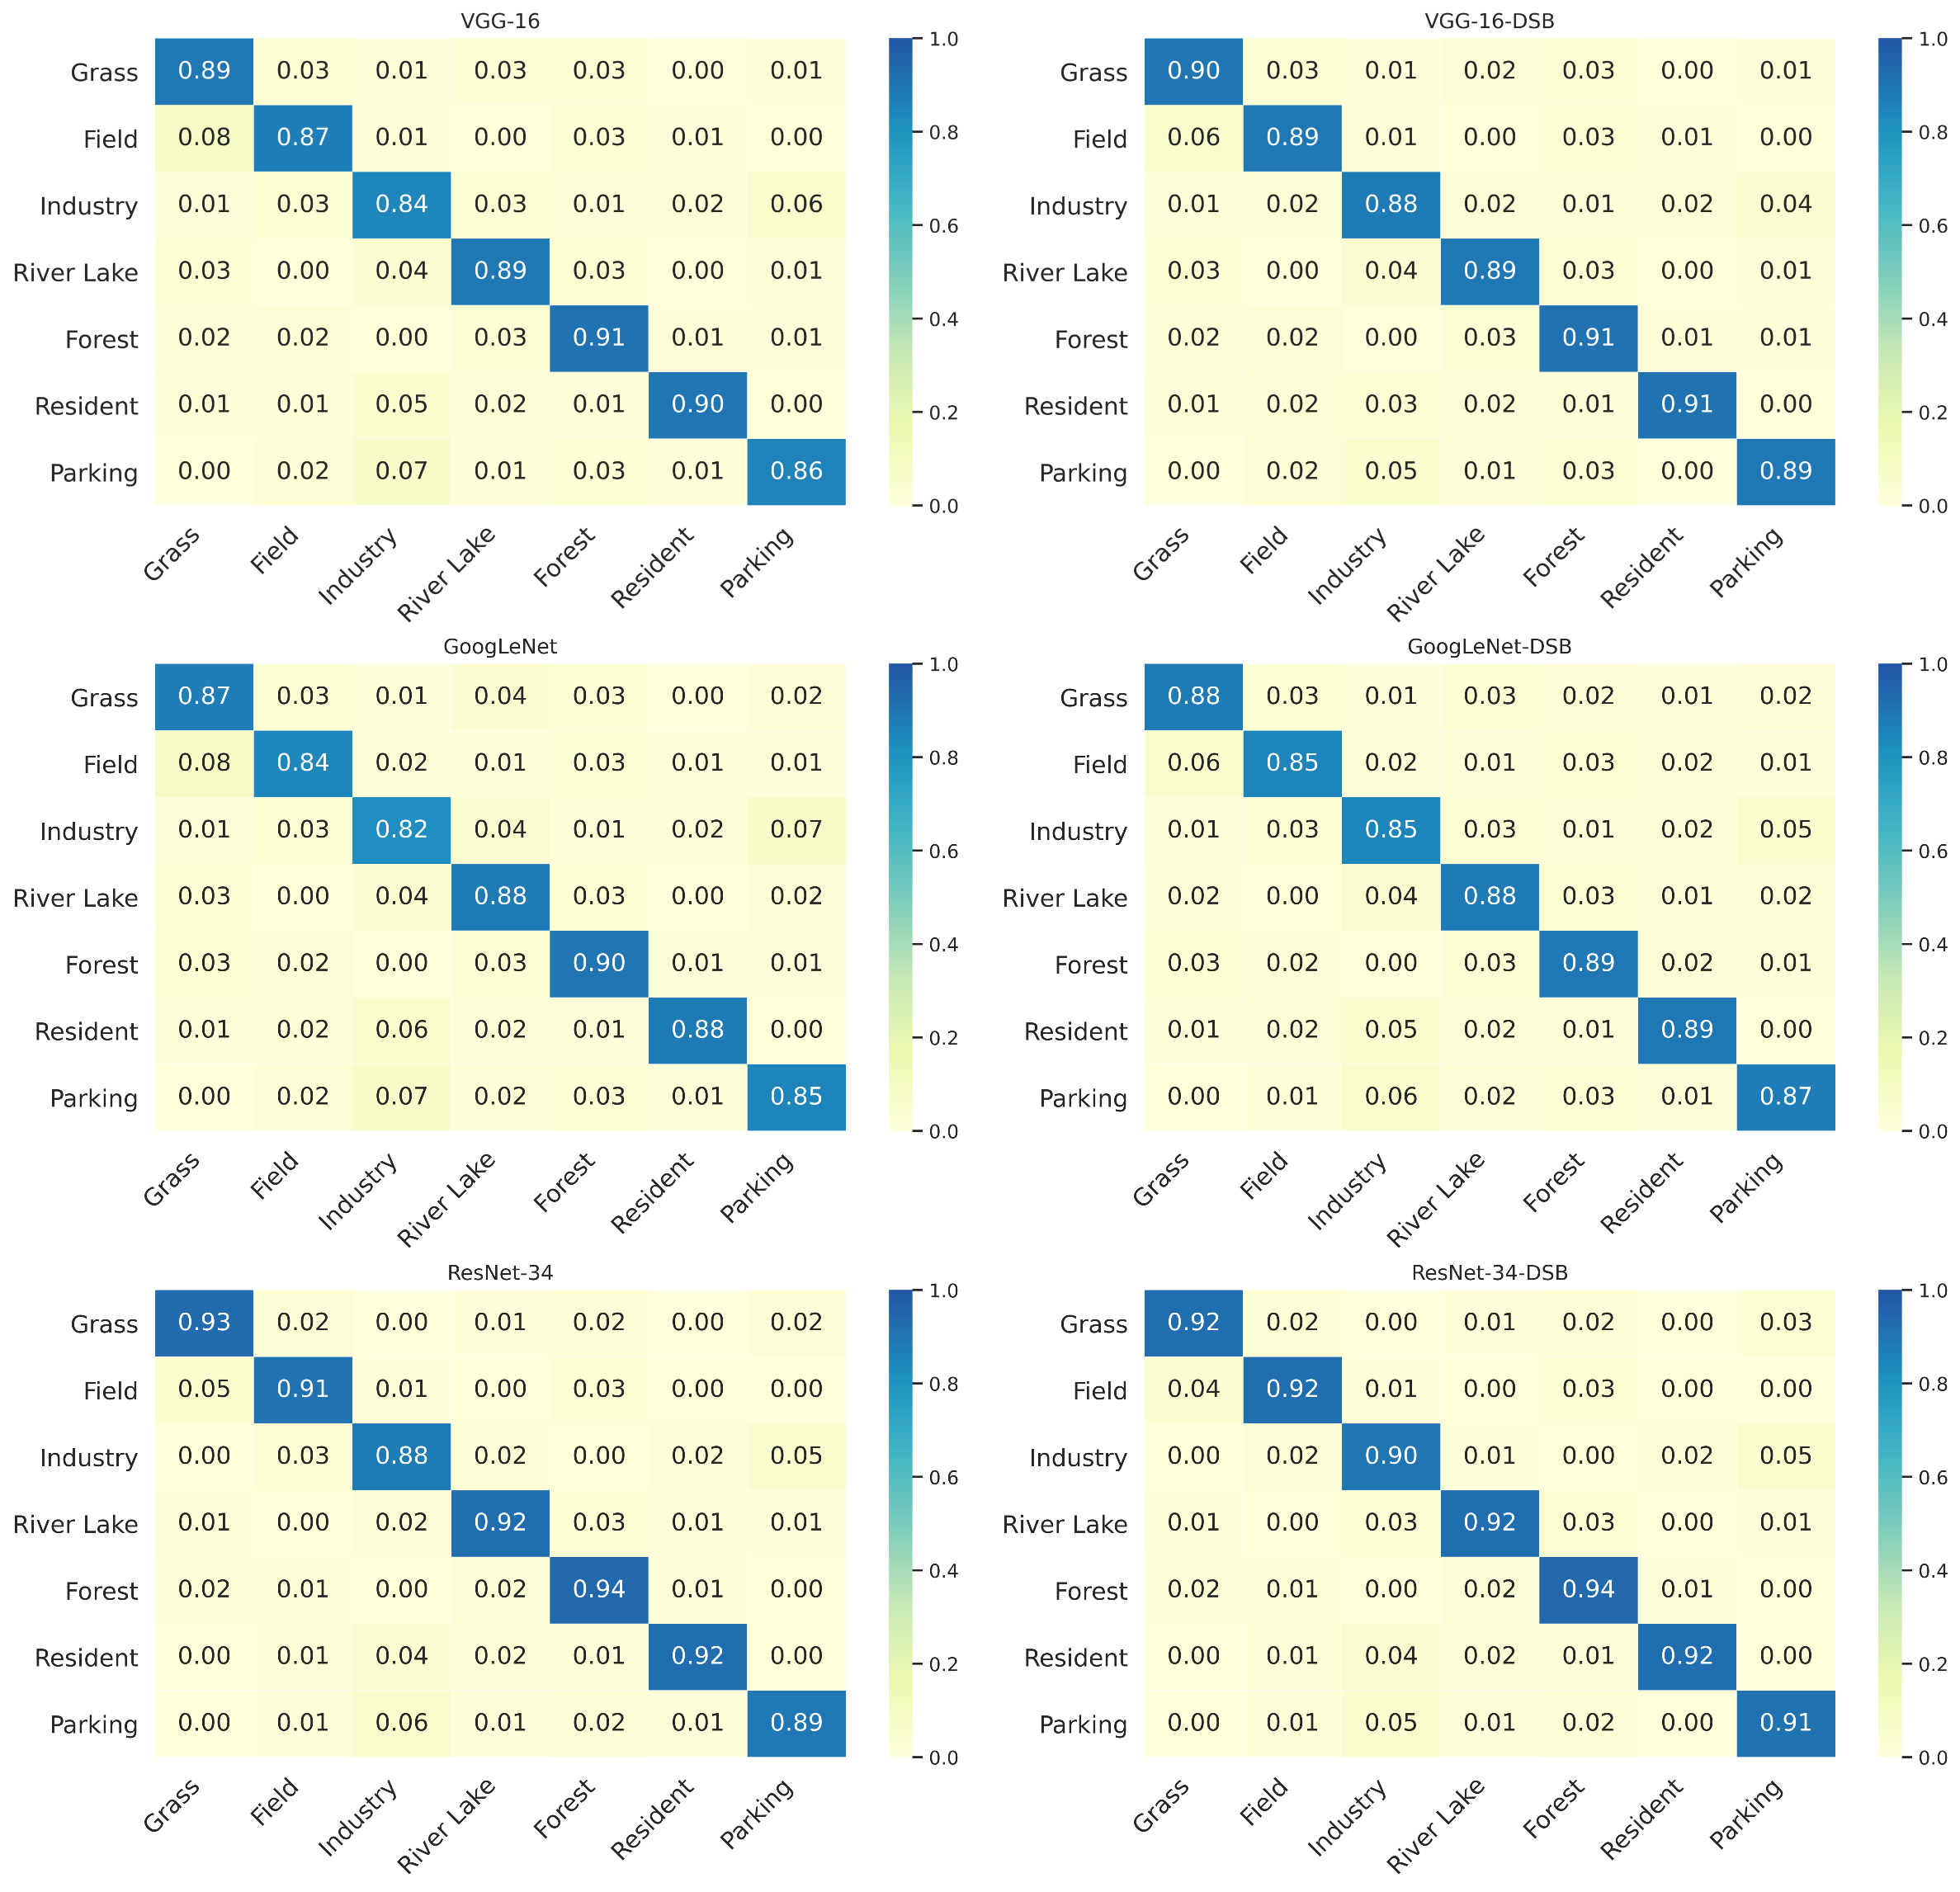
\includegraphics[width=1\columnwidth]{nfig32}
\vskip -0.1in
\caption{\textbf{Left column:} confusion matrix of VGG-16, GoogLeNet, and ResNet-34 on the RSSCN7 dataset. \textbf{Right column:} confusion matrix of VGG-16-DSB, GoogLeNet-DSB, and ResNet-34-DSB on the RSSCN7 dataset.}
\label{fig32}
\end{center}
\vskip -0.17in
\end{figure*}

\begin{figure*}[t]
\begin{center}
%\vskip -0.3in
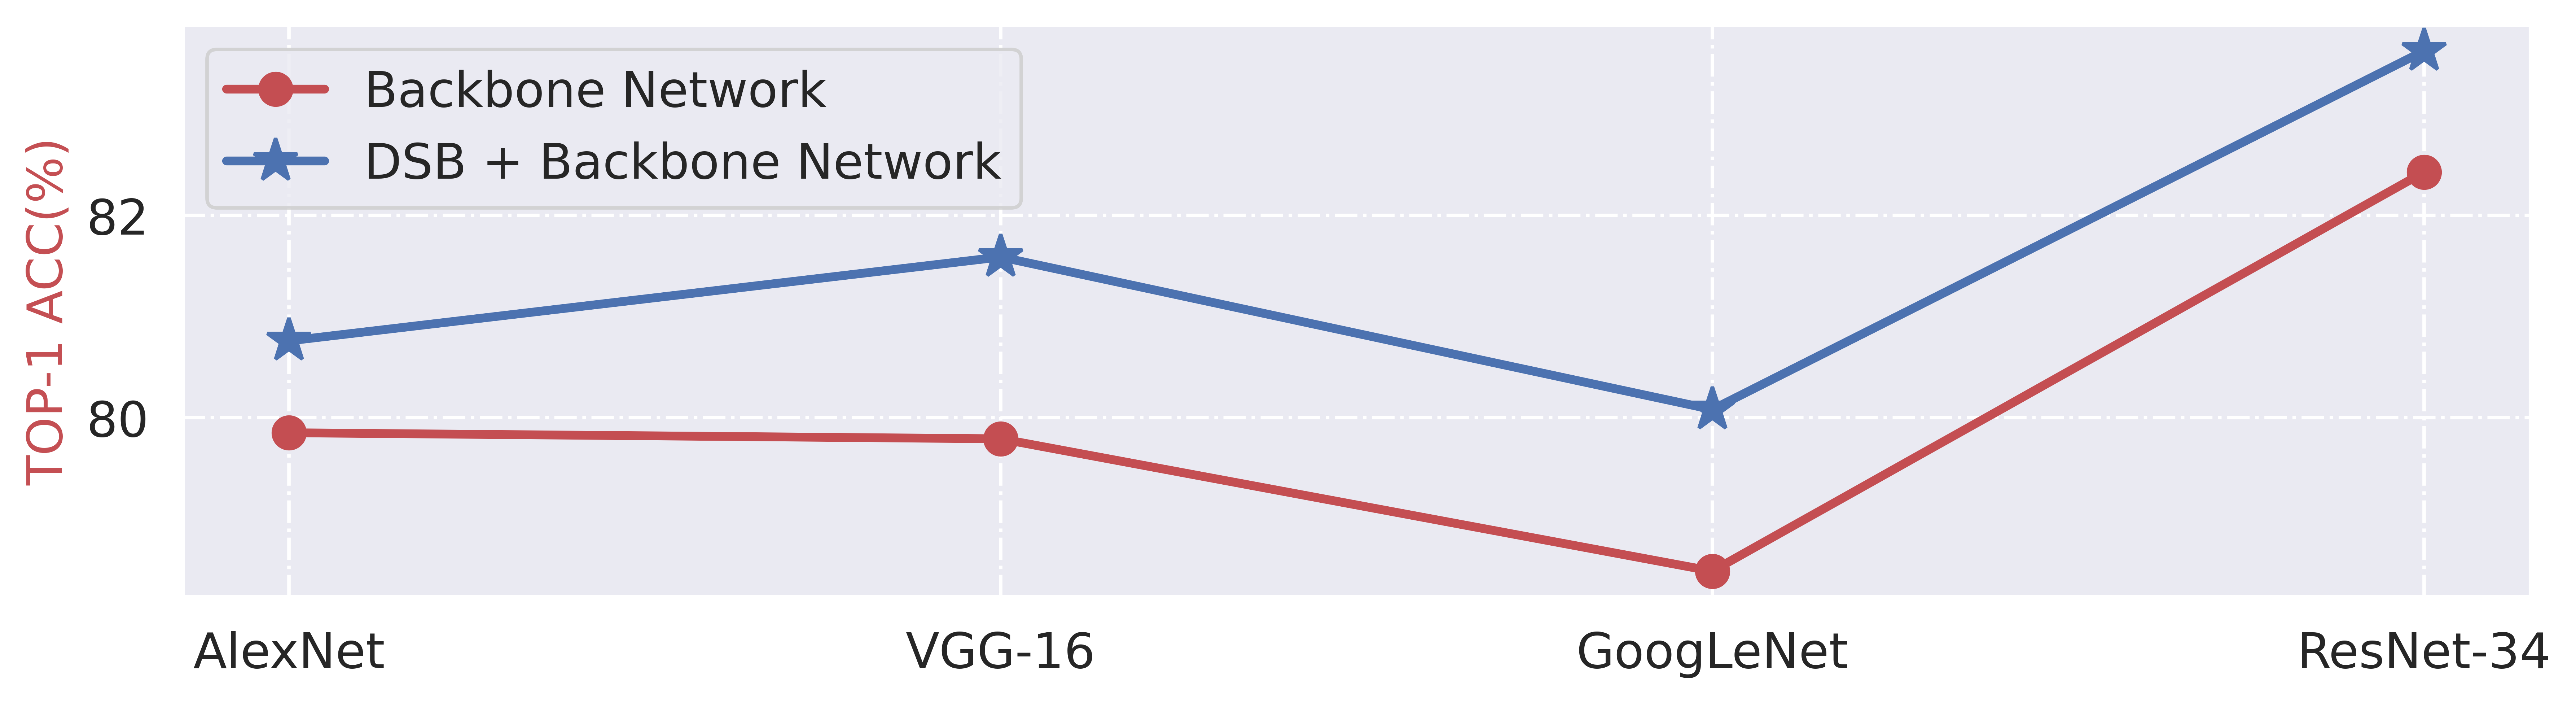
\includegraphics[width=1\columnwidth]{fig33}
\vskip -0.1in
\caption{Comparison of four backbone networks before and after combining with dynamic semantic scale-balanced learning on dataset NWPU-RESISC45.}
\label{fig33}
\end{center}
%\vskip -0.05in
\end{figure*}

\subsubsection{Results on NWPU-RESISC45}

We significantly improved the performance of multiple backbone networks by employing dynamic semantic-scale-balanced learning on the NWPU-RESISC45 dataset, and the experimental results are illustrated in Figure \ref{fig33}. It can be observed that the overall performance of VGG-16-DSB is $1.8$\% higher than that of VGG-16. Meanwhile, dynamic semantic-scale-balanced learning improves the overall performance of GoogLeNet and ResNet-34 by $1.6$\% and $1.2$\%.

\textbf{Experiment Summary.} On two remote sensing image datasets with balanced sample numbers, our method shows significant improvements on common backbone networks. The experimental results show that semantic scale imbalance exists in the remote sensing image dataset and affects the performance of deep neural networks to some extent. Remote sensing images hold great promise for applications in agriculture, industry, and the military, so it is crucial to promote the fairness of deep neural networks on remote sensing images.

%%%%%%%%%%%%%%%%%%%%%%%%%%%%
%%.             END-Remote sensing     %%%%%%%%%
%%%%%%%%%%%%%%%%%%%%%%%%%%%%
\section{Pseudo Code for Sample Volume\label{C}}

An image can be considered as a point in the sample space, and the dimension of the sample space is the same as the number of image pixel points. The manifold distribution law considers that multiple images from a class are distributed around a low-dimensional manifold in the sample space. We calculate for each class the volume of its corresponding manifold and call it the sample volume. We provide the pseudo code for the calculation of the sample volume in Algorithm \ref{alg1}. In this work, we resize the image to (16, 16, 3) and then calculate the sample volume after flattening.


\begin{algorithm}[h]
   \caption{Calculation of Sample Volume}
   \label{alg1}
\begin{algorithmic}
   \STATE {\bfseries Input:} Training set $D = \left\{ {\left( {{x_i},{y_i}} \right)} \right \}_{i = 1}^M$ with the total number $C$ of classes
   \STATE {\bfseries Onput:} Sample volumes for all classes
   \FOR{$j=1$ to $C$}
   \STATE Select the sample set ${D_j} = \left\{ {\left( {{x_i},{y_i}} \right)} \right\}_{i = 1}^{{m_j}}$ for class $j$ from $D$, ${m_j}$ is the number of samples for class $j$
   \STATE Resize the image to ($imagesize$, $imagesize$, 3)
   \STATE Flatten the image into a vector of length $d = imagesize \times imagesize \times 3$ and store it in ${Z_j} = \left[ {{z_1},{z_2}, \ldots ,{z_{{m_j}}}} \right] \in {\mathbb{R}^{d \times {m_j}}}$
   \STATE ${Z_j} = {Z_j} - N\!um\!P\!y.mean\left( {{Z_j}, {\rm{1}}} \right)$
   \STATE Calculate the covariance matrix ${\Sigma _j} = \frac{1}{{{m_j}}}{Z_j}Z_j^T$
   \STATE Calculate the sample volume $V\!ol\left( {{\Sigma _j}} \right) = \frac{1}{2}{\log _2}\det \left( {I + d{\Sigma _j}} \right)$ for class $j$
   \ENDFOR
\end{algorithmic}
\end{algorithm}



\section{Dynamic Semantic-Scale-Balanced Learning}

\subsection{DSB-NSM, DSB-ST and DSB-Focal Loss\label{D.1}}


Given the embedding $z$ of a sample and label $y_{i}$, the dynamic semantic-scale-balanced (DSB) loss can be expressed as:\begin{equation}
D\!S\!B( {z,{y_i}} ) = \frac{1}{{{S_i}}}L( {z,{y_i}} ),i = 1,2, \ldots ,C,
\end{equation}where ${y_i}$ is the label of the sample from class $i$. To show how to combine the general loss to generate the dynamic semantic-scale-balanced loss, we improve the NormSoftmax (NSM) cross-entropy loss and SoftTriple (ST) loss. NormSoftmax removes the bias term in the last linear layer and an L2 normalization module is added to the inputs and weights before the SoftMax loss. $[{{w_1},{w_2},\cdots ,{w_C}}] \in {\mathbb{R}^{d \times C}}$ is the last fully connected layer, then the DSB-NSM with temperature $\sigma$ generated by embedding $z$ can be written as:\begin{equation}
D\!S\!B\!-\!N\!S\!M( {z,y_i} ) =  - \frac{1}{{{S_i}}}\log ( {\frac{{\exp ( {{{w_{{y_i}}^Tz} \mathord{/
 {\vphantom {{w_{{y_i}}^Tz} \sigma }} 
 \kern-\nulldelimiterspace} \sigma }} )}}{{\sum\nolimits_{j = 1}^C {\exp ( {{{w_j^Tz} \mathord{/
 {\vphantom {{w_j^Tz} \sigma }} 
 \kern-\nulldelimiterspace} \sigma }} )} }}} ).
\end{equation}The SoftTriple loss combined with the semantic-scale-balanced term is expressed as 
\begin{equation}
D\!S\!B\!-\!S\!T( {z,y_i} )=- \frac{1}{{{S_i}}}\!\log ( {\frac{{\exp ( {\lambda ( {{{D'}_{z,y_i}} - \delta } )} )}}{{\exp ( {\lambda ( {{{D'}_{z,y_i}} - \delta } )} ) + \sum\nolimits_{j \ne y} {\exp ( {\lambda {{D'}_{i,j}}} )} }}} ),
\end{equation}where $\lambda$ is a scaling factor and $\delta$ is a hyperparameter. The relaxed similarity between embedding $z$ and class $c$ is defined as ${{D'}_{z,c}} = \sum\limits_k {\frac{{\exp ( {\frac{1}{\gamma }z^Tw_c^k} )}}{{\sum\nolimits_k {\exp ( {\frac{1}{\gamma }z^Tw_c^k} )} }}} z^T\!w_c^k$, where $k$ is the number of centers for each class. 

The purpose of Focal loss is to apply small loss weights to samples with high classification confidence, thus increasing the proportion of loss of hard samples with low classification confidence to the overall loss. The $\alpha$-balanced variant of Focal loss regulates the proportion of loss among samples while assigning different weights to each class, which is denoted as $FL\left( {{p_t}} \right) =  - {\alpha _t}{\left( {1 - {p_t}} \right)^\gamma }\log \left( {{p_t}} \right)$, where $p_t$ is the probability that the sample belongs to the true class. When ${\alpha _t} = \frac{1}{{{S_i}}}$, Focal loss is transformed into DSB-Focal loss.






\subsection{Dynamic Re-Weighting Training Framework\label{D.2}}



Given the training samples $X = \left[ {{x_1},{x_2},\ldots,{x_N}} \right]$ containing $C$ classes and corresponding labels $Y = \left[ {{y_1},{y_2},\ldots,{y_N}} \right]$, the number of samples per class is ${N_i}\left( {i = 1,2 \ldots ,C} \right)$, and the total number of samples is $N$. The d-dimensional features extracted by the CNNs are denoted as $Z = \left[ {{z_1},{z_2},\ldots,{z_N}} \right] \in {\mathbb{R}^{d \times N}}$. In this work, we conduct experiments for two types of tasks, image classification and deep metric learning. In the field of deep metric learning, $64$-dimensional features are generally adopted, while the features extracted by the network in image classification tasks tend to be of high dimensionality. For example, the feature dimension extracted by ResNet-50 is $2048$, which will occupy more video memory. Therefore, when saving historical features in the classification task, one-dimensional average pooling is performed on all features to reduce the feature dimension to $64$, which is consistent with the common feature dimension in the field of deep metric learning while preserving the geometry of the distribution (because the pooling operation is translation invariant, rotation invariant, and scale invariant).

In the following, we describe the three-stage training framework in detail.



\begin{figure*}[h] % 纵向8行,图片靠右,宽度12.5em
\begin{center}
%\vskip -0.01in
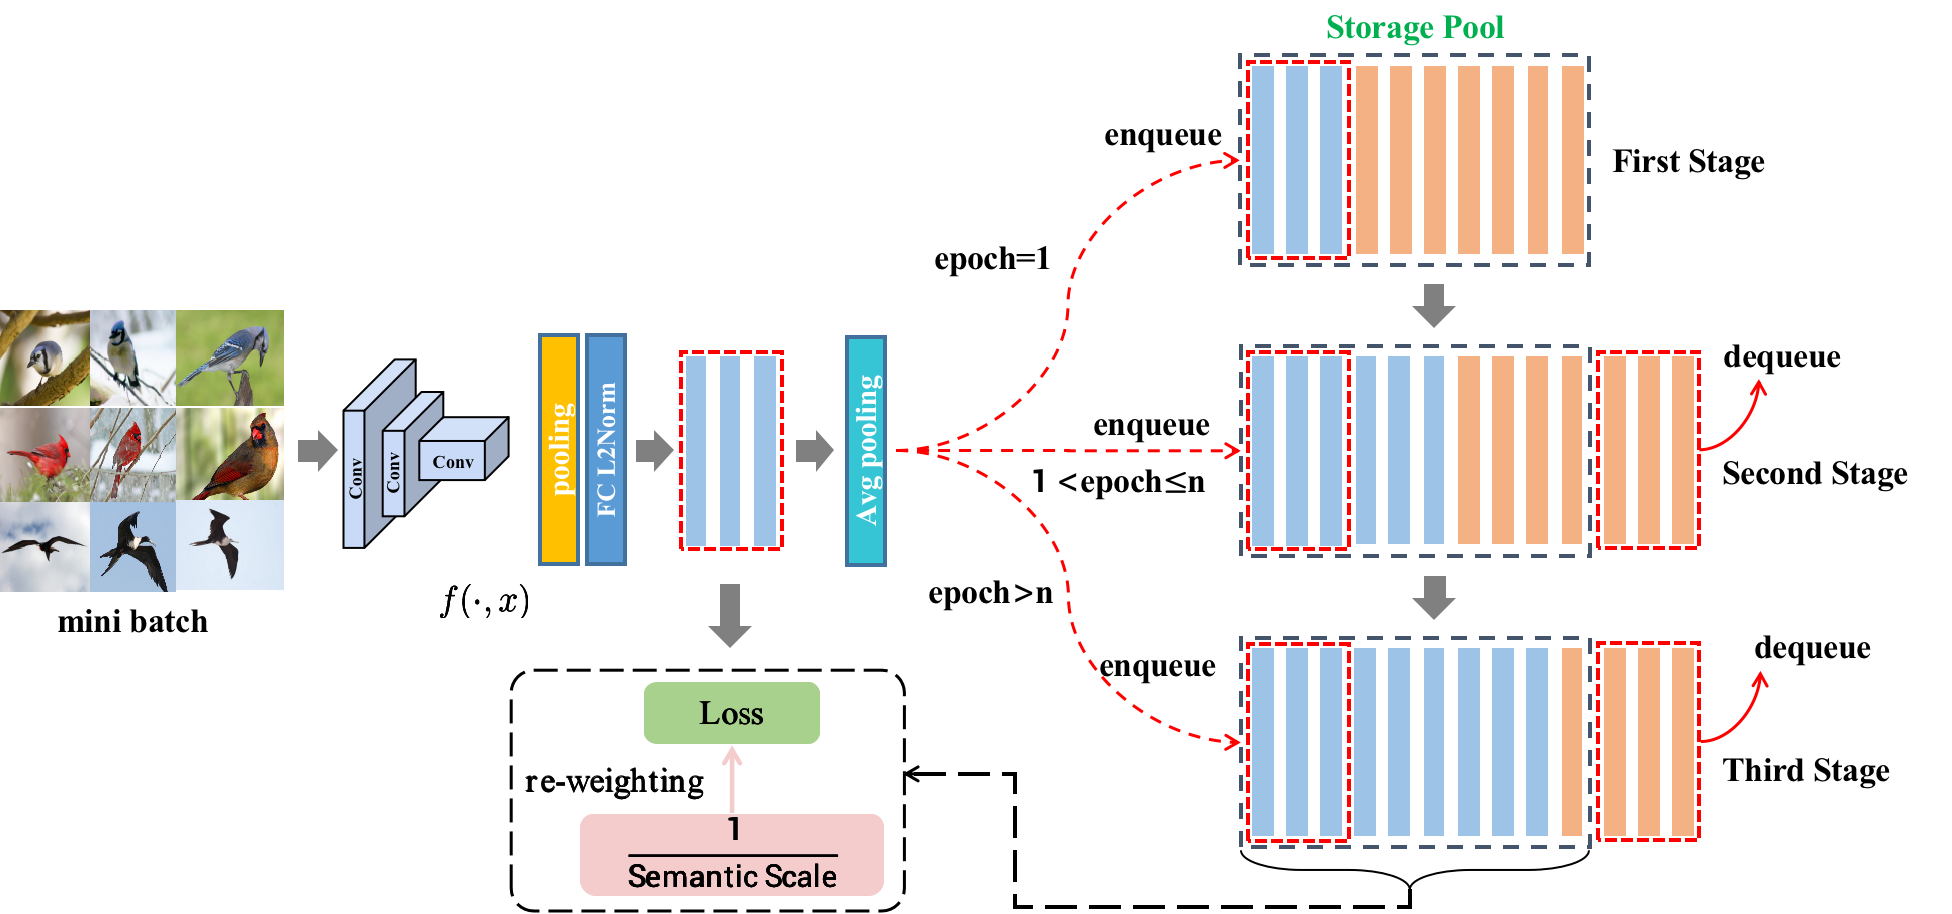
\includegraphics[width=1\columnwidth]{fig7}
\vskip -0.05in
\caption{The three-stage training framework. The features in the storage pool are continuously updated during training and semantic scales are calculated using all the latest features.}
\label{fig7}
\end{center}
\vskip -0.1in
\end{figure*}



The three-stage training framework is shown in Figure \ref{fig7}:

\textbf{(1)} In the \textbf{first stage}, all the features and labels generated by the 1st epoch are stored in $Q$, which is denoted as:
\[Q = \left[ {\begin{array}{*{20}{c}}
Z\\
Y
\end{array}} \right] = \left[ {\begin{array}{*{20}{c}}
{{Z_{11}}}& \cdots &{{Z_{1N}}}\\
 \vdots & \ddots & \vdots \\
{{Z_{d1}}}& \cdots &{{Z_{dN}}}\\
{{y_1}}& \cdots &{{y_N}}
\end{array}} \right] \in {\mathbb{R}^{\left( {d + 1} \right) \times N}}.\]
$Q$ contains the features and labels of all samples, but in the early stage of training, the historical features have a large drift from the current features and cannot be used directly to calculate the semantic scale.

\iffalse
\begin{wrapfigure}[13]{r}{18.8em} % 纵向8行,图片靠右,宽度12.5em
\begin{center}
\vskip -0.26in
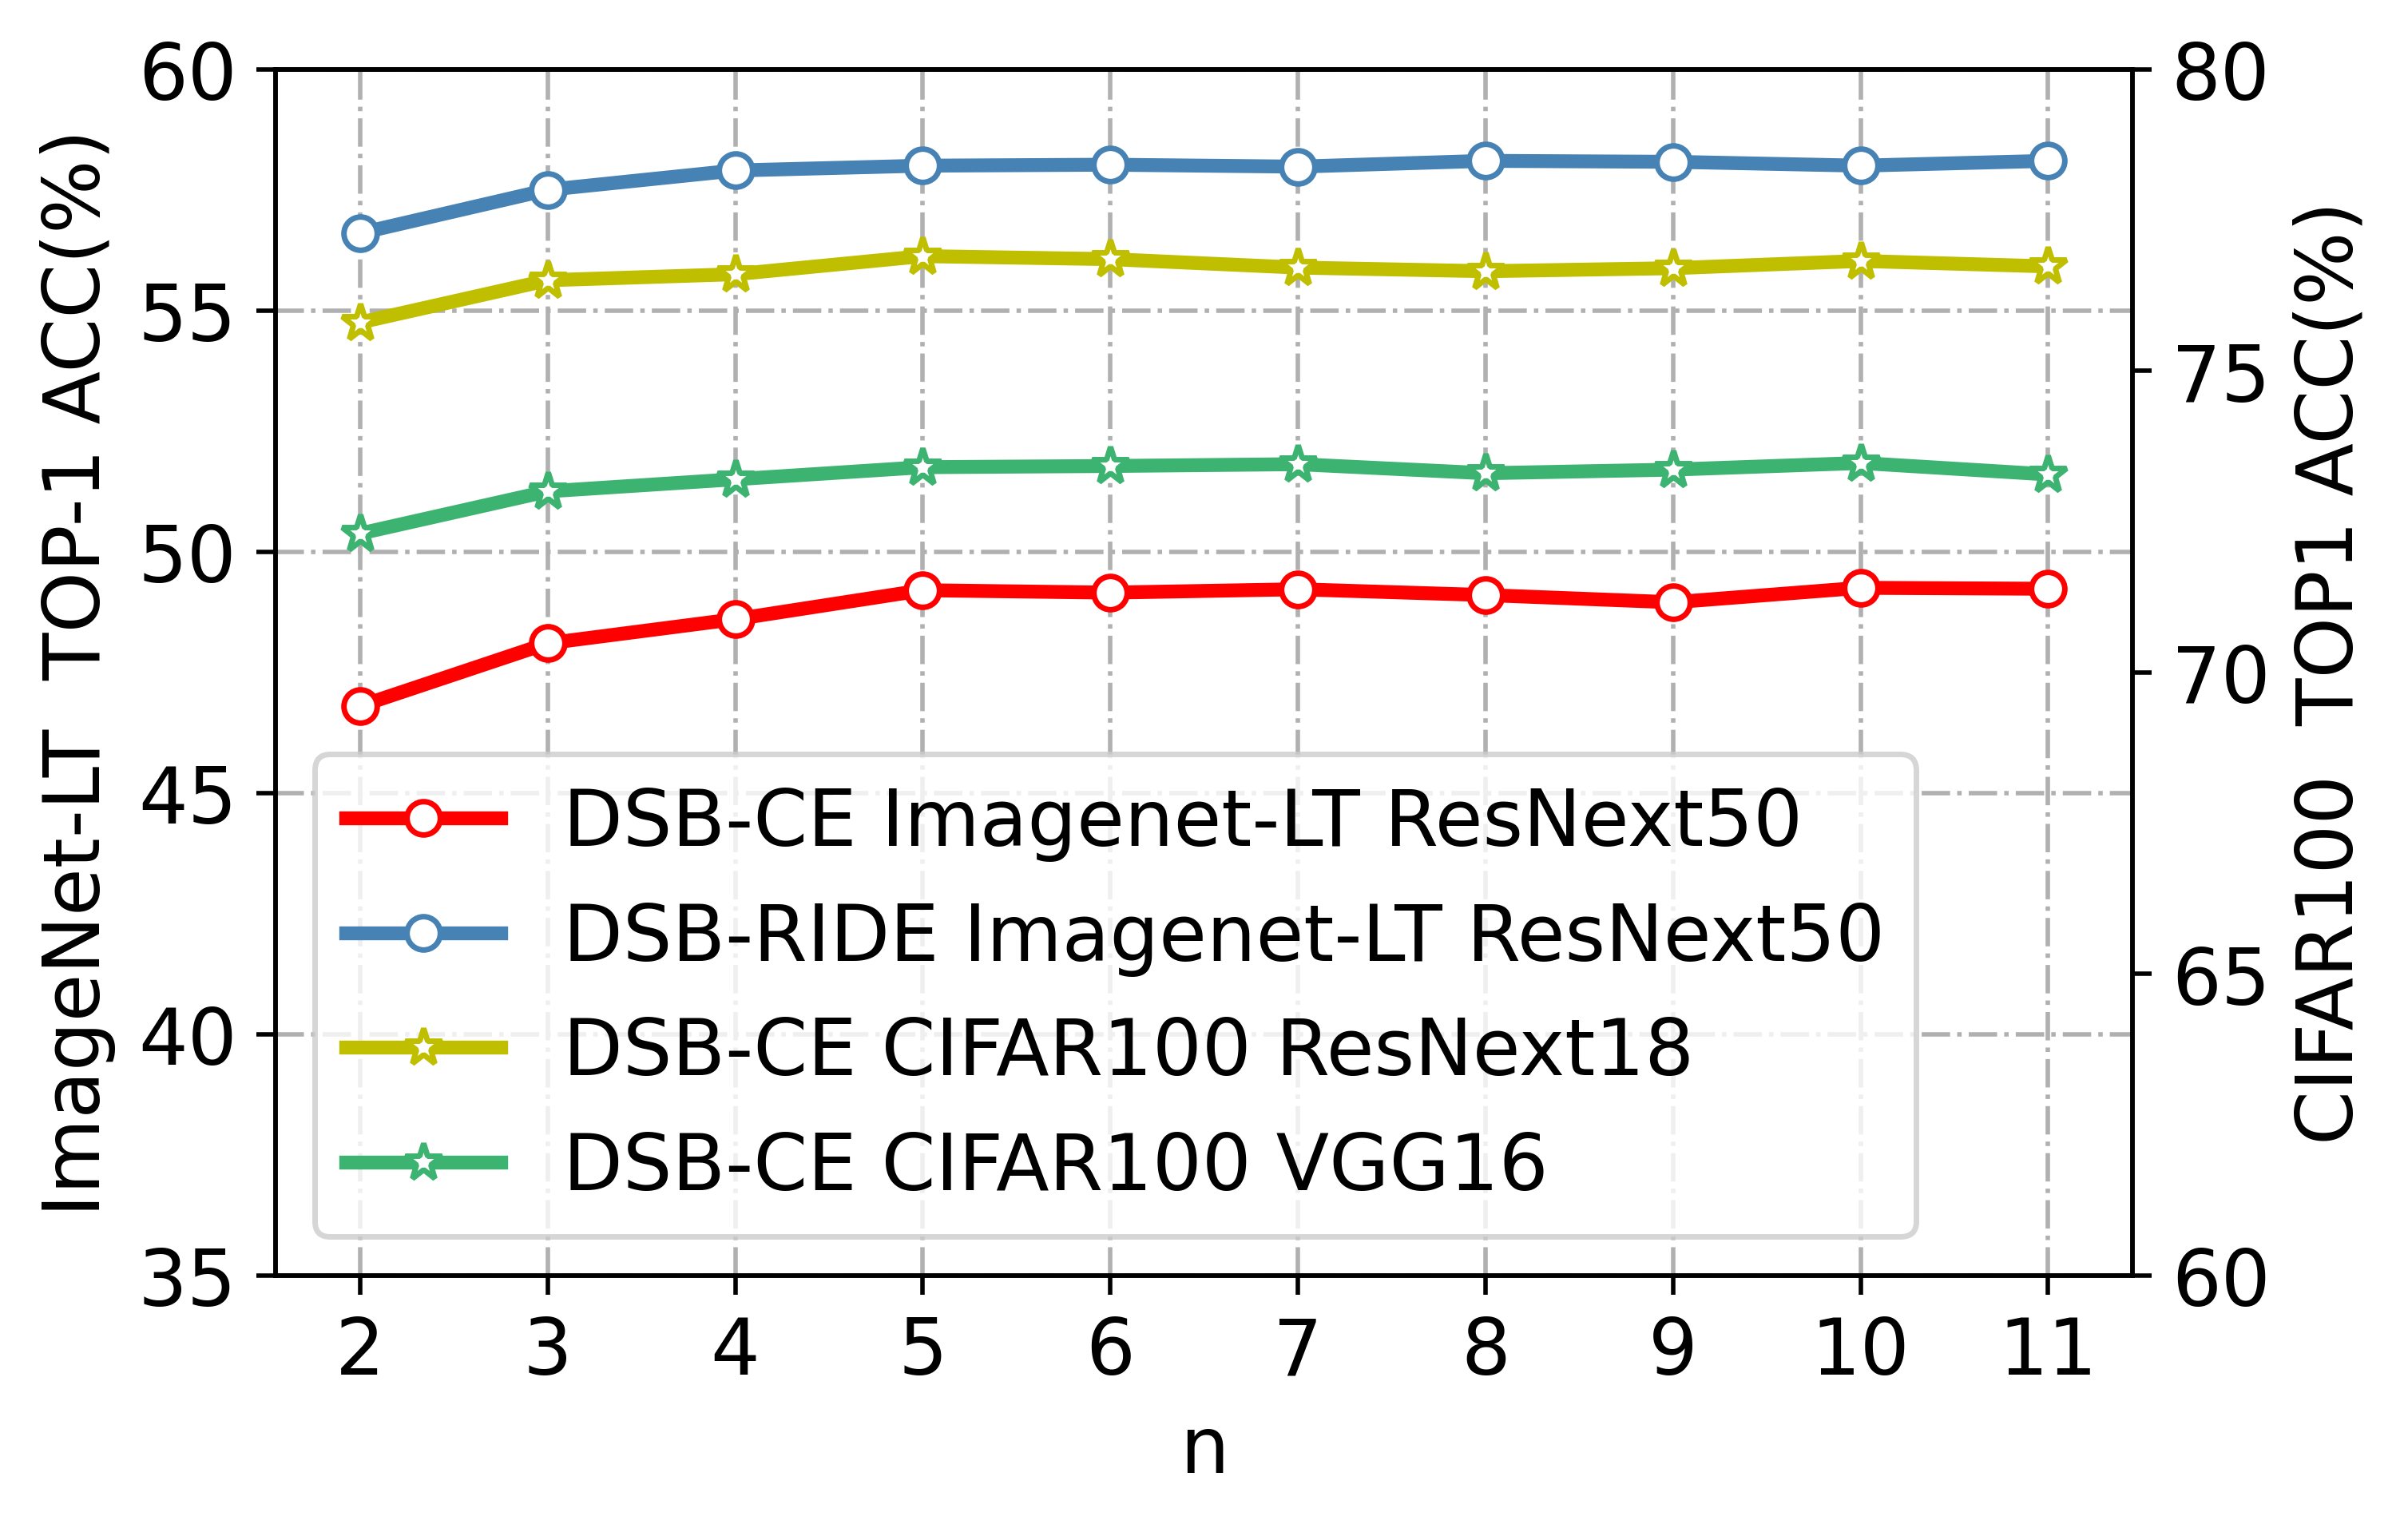
\includegraphics[width=0.48\columnwidth]{fig8}
\vskip -0.15in
\caption{The performance of different models with different losses on different datasets for different values of $n$.}
\label{fig8.1}
\end{center}
\end{wrapfigure}
\exercise
\fi


\textbf{(2)} The \textbf{second stage} corresponds to epoch 2 to epoch $n$. At each iteration, the oldest mini-batch features and labels in $Q$ are removed and those generated by the current iteration are stored. The goal is to continuously update the features in $Q$ until the feature drift is small enough. We set $n$ to 5 in our experiments, and the original loss function is used in the first two stages. Figure \ref{fig8} shows the effect of $n$ on the model performance. A larger $n$ does not hurt the model performance, but only takes a little more time. Experience suggests that setting $n$ to 5 is sufficient. 

\textbf{(3)} The \textbf{third stage} corresponds to epoch $>$ $n$. At each iteration, the semantic scales are calculated using the features in $Q$ after updating $Q$, and the original loss is re-weighted.


Algorithm \ref{alg2} shows how to apply the dynamic re-weighting training framework by taking DSB-ST loss as an example.



\begin{algorithm}[h]
   \caption{Dynamic Re-Weighting Training Framework}
   \label{alg2}
\begin{algorithmic}
   \STATE {\bfseries Input:} Training set $D = \{ {\left( {{x_i},{y_i}} \right)} \}_{i = 1}^M$, total training epochs $N_{epoch}$, defined encoder is model()
   \STATE Initialize the queue $Q$
   \FOR{$epoch=1$ to $N_{epoch}$}
   \FOR{$iteration=0$ to $\frac{M}{{batchsize}}$}
   \STATE Sample a mini-batch $\{ {\left( {{x_i},{y_i}} \right)} \}_{i = 1}^{batchsize}$ from $D$
   \STATE Calculate features $F = \left[ {{f_1}, \ldots ,{f_i}, \ldots ,{f_{batchsize}}} \right],{f_i} = \rm{model}\left( {{x_i}} \right),i = 1, \ldots ,batchsize$
   \STATE Store $F$ and label $y$ into $Q$: $enqueue\left( {Q,\left[ {F,y} \right]} \right)$
   \IF {$epoch < n$}  
   \IF {$epoch > 1$} 
   \STATE Dequeue the oldest mini-batch features from $Q$
   \ENDIF
   \STATE Calculate loss $L = S\!o\!ftTripleloss\left( {F,y} \right)$
   \ELSE
   \STATE Dequeue the oldest mini-batch features from $Q$
   \STATE Calculate loss $L = D\!S\!B.S\!o\!ftTripleloss\left( {F,y} \right)$
   \ENDIF
   \STATE Perform back propagation: $L$.backward()
   \STATE optimizer.step()
   \ENDFOR
   \ENDFOR
\end{algorithmic}
\end{algorithm}




The proposed three-stage training framework overcomes the difficulty of not being able to calculate class-wise semantic scales during training due to the limited number of samples per batch. In fact, there is a simple and brute-force method to achieve the goal of calculating class-wise semantic scales in real time, which is to extract features of all samples using the current model after each iteration. However, this would take a lot of time, for example, when training ImageNet with batch size of 512, one epoch contains about 2,500 iterations. This also means that all features need to be extracted 2,500 times, which is unacceptable.

\begin{table*}[h]
\renewcommand\arraystretch{1.3}
\setlength{\tabcolsep}{22pt} %修改行距
\caption{Comparison of DSB-ST and SoftTriple in terms of memory consumption and training speed. The speed is measured by the average number of iterations per second. The additional video memory consumption due to our method is almost negligible.}
\label{table10}
\vskip 0.1in
\centering   
\begin{tabular}{ c | c c| c c}
\hline \toprule 
\multicolumn{1}{c}{ }  &   \multicolumn{2}{|c|}{GPU Memory}  &   \multicolumn{2}{c}{Training speed} \\ \hline
\multicolumn{1}{c|}{Dataset} &   \,\,\,SoftTriple  & DSB-ST  &  \,\,SoftTriple  & DSB-ST \\ \toprule
\multicolumn{1}{c|}{ImageNet-LT}  &  \,\,\,24.29 GB  &  24.75 GB  & \,\,6.01 it/s  & 5.56 it/s \\ \hline
\multicolumn{1}{c|}{iNaturalist2018}  &  \,\,\,45.13 GB  &  46.88 GB  & \,\,3.32 it/s  & 3.03 it/s \\ \hline
\multicolumn{1}{c|}{Cars196}  &  \,\,\,3491 MB  &  4097 MB  & \,\,20.21 it/s  & 18.95 it/s \\ \hline
\multicolumn{1}{c|}{CUB-2011}  &  \,\,\,3225 MB  &  3647 MB  & \,\,21.95 it/s  & 18.58 it/s \\ \hline
\multicolumn{1}{c|}{Mini-ImageNet}  &  \,\,\,3491 MB  &  3713 MB  & \,\,23.34 it/s  & 20.36 it/s \\
 \bottomrule \hline
\end{tabular}
\vskip -0.1in
\end{table*}

Our method causes almost no reduction in training speed. In terms of video memory consumption, even the extracted features of a million-level dataset like ImageNet can all be placed on one graphics card (about 6,000 MB of video memory is needed). In this work, we use 4 NVIDIA 2080Ti GPUs to train all the models. A comparison of the video memory consumption and training speed for some experiments is shown in Table \ref{table10}. It can be noticed that the consumption of our method is negligible for the video memory, and the training speed is about 90\% of the original method.



\section{Volume Formula for the Low-Dimensional Parallel Hexahedron in the High-Dimensional Space\label{E}}
In Section \ref{3.2} of the main content, we deduce from the singular value decomposition of the matrix $Z = \left[ {{z_1},{z_2}, \ldots ,{z_m}} \right] \in {\mathbb{R}^{d \times m}}$ composed of features that the volume $V\!ol( Z )$ of the subspace spanned by $z_i$ is proportional to $\sqrt {\det ( {\frac{1}{m}\!Z\!{Z^T}} )}$. Here, we assume that in $\mathbb{R}^d$, given $m$ d-dimensional vectors, these vectors will define a parallel hexahedron in $\mathbb{R}^n$. The problem is how to calculate the parallel hexahedron. For example, consider two vectors 
\[{z_1} = \left[\! {\begin{array}{*{20}{c}}
1\\
2\\
3
\end{array}} \!\right],{z_2} = \left[\! {\begin{array}{*{20}{c}}
3\\
2\\
1
\end{array}}\! \right].\]

The parallel hexahedron defined by these two vectors is a parallelogram in $\mathbb{R}^3$. We want to find a formula to calculate the area of the parallelogram. (Note that the true three-dimensional volume of the planar parallelogram is 0, just as the length of the point is 0 and the area of the line is 0. Here, we are trying to measure the two-dimensional ``volume" of the parallelogram.)

Next we will introduce two special cases of parallel hexahedral volume, for a single vector \[z = \left[\!\! {\begin{array}{*{20}{c}}
{{a_1}}\\
 \vdots \\
{{a_n}}
\end{array}} \!\!\right] \in {\mathbb{R}^n},\]
whose parallel hexahedral is itself. Here ``volume" means the length of the vector, and according to the Pythagorean theorem its volume is
\begin{equation}
\sqrt {a_1^2 +  \cdots  + a_n^2}. 
\end{equation} 


Another case is to give $n$ vectors in ${\mathbb{R}^n}$. Suppose that these $n$ vectors are
\[{z_1} = \left[\!\!\! {\begin{array}{{c}}
{{a_{11}}}\\
 \vdots \\
{{a_{n1}}}
\end{array}}\!\!\! \right], \ldots ,{z_n} = \left[\!\!\! {\begin{array}{{c}}
{{a_{1n}}}\\
 \vdots \\
{{a_{nn}}}
\end{array}}\!\!\! \right],\]
we can know that the volume of the resulting parallel hexahedron is \begin{equation}\left| {\left. {\det \!\left[\! {\begin{array}{*{20}{c}}
{{a_{11}}}& \cdots &{{a_{1n}}}\\
 \vdots & \ddots & \vdots \\
{{a_{n1}}}& \cdots &{{a_{nn}}}
\end{array}} \!\right]} \right|.} \right.\end{equation}


In the non-special case, the formula for the volume of a low-dimensional parallel hexahedron in a high-dimensional space will contain Results (7) and (8). Here, we first present the final formula and then discuss why it is reasonable. Write the $k$ vectors ${z_1}, \ldots ,{z_k}$ in ${\mathbb{R}^n}$ as column vectors. Let \[Z = \left[ {{z_1}, \ldots ,{z_k}} \right] \in {\mathbb{R}^{n \times k}},\]
and the volume of the parallel hexahedron derived from the vectors ${z_1}, \ldots ,{z_k}$ is \[\sqrt {\det\! \left[ {{Z^T}\!Z} \right]}. \]

We now discuss why $\sqrt {\det\! \left[ {{Z^T}\!Z} \right]}$ must be the volume in the general case.

\begin{lemma}
\emph{For a matrix $Z = \left[ {{z_1}, \ldots ,{z_k}} \right]$, we can get} \[{Z^T}\!Z = \left[\! {\begin{array}{*{20}{c}}
{{{\left| {{z_1}} \right|}^2}}&{{z_1} \cdot {z_2}}& \cdots &{{z_1} \cdot {z_k}}\\
 \vdots & \vdots & \ddots & \vdots \\
{{z_k} \cdot {z_1}}&{{z_k} \cdot {z_2}}& \cdots &{{{\left| {{z_k}} \right|}^2}}
\end{array}} \!\right],\]
\emph{where ${{z_i} \cdot {z_j}}$ denotes the dot product of the vectors $z_i$ and $z_j$ and $\left| {{z_i}} \right| = \sqrt {{z_i} \cdot {z_i}}$ denotes the length of the vector.}

\emph{The proof of Lemma 1 needs to focus only on}
\[{Z^T}\!Z = \left[\!\! {\begin{array}{*{20}{c}}
{z_1^T}\\
 \vdots \\
{z_k^T}
\end{array}}\!\! \right]\left[ {{z_1}, \cdots ,{z_k}} \right].\]

\emph{If we apply any linear transformation that preserves angularity and length in $\mathbb{R}^n$ (in other words, if we perform a rotation operation on $\mathbb{R}^n$), the numbers $\left| {{z_i}} \right|$ and ${{z_i} \cdot {z_j}}$ do not change. The multiple sets of all linear transformations that preserve angle and length in $\mathbb{R}^n$ form a group, called the orthogonal group and denoted as ${\rm O}\!\left( n \right)$. This allows us to reduce the problem to that of finding the volume of a parallel hexahedron in $\mathbb{R}^k$.}
\end{lemma}


\emph{\textbf{Proof.}} \,It is known that \[ \sqrt {\det\! \left[ {{Z^T}\!Z} \right]} = \sqrt {\det \left[\!\! {\begin{array}{*{20}{c}}
{{{\left| {{z_1}} \right|}^2}}&{{z_1} \cdot {z_2}}& \cdots &{{z_1} \cdot {z_k}}\\
 \vdots & \vdots & \ddots & \vdots \\
{{z_k} \cdot {z_1}}&{{z_k} \cdot {z_2}}& \cdots &{{{\left| {{z_k}} \right|}^2}}
\end{array}}\!\!\right]}.\] To prove that the above equation must be the formula for the volume, we first consider a set of standard basis of $\mathbb{R}^n$: 
\[{e_1} = \left[\! {\begin{array}{*{20}{c}}
1\\
0\\
 \vdots \\
0
\end{array}} \!\right],{e_2} = \left[\! {\begin{array}{*{20}{c}}
0\\
1\\
 \vdots \\
0
\end{array}} \!\right], \ldots ,{e_n} = \left[\! {\begin{array}{*{20}{c}}
0\\
0\\
 \vdots \\
1
\end{array}} \!\right].\]

According to Lemma 1, we are able to find a rotation of $\mathbb{R}^n$, which is able to maintain both length and angle, and also rotate our vectors ${{z_1}, \ldots ,{z_k}}$ such that they can be fully represented linearly by the first $k$ standard vectors ${{e_1}, \ldots ,{e_k}}$ (which is geometrically reasonable). After the rotation, the latter $n\!-\!k$ dimensions of each vector zi are 0. Therefore we can think of our parallel hexahedron as consisting of $k$ vectors in $\mathbb{R}^k$ and we already know how to calculate it, which is \[\sqrt {\det \left[\!\! {\begin{array}{*{20}{c}}
{{{\left| {{z_1}} \right|}^2}}&{{z_1} \cdot {z_2}}& \cdots &{{z_1} \cdot {z_k}}\\
 \vdots & \vdots & \ddots & \vdots \\
{{z_k} \cdot {z_1}}&{{z_k} \cdot {z_2}}& \cdots &{{{\left| {{z_k}} \right|}^2}}
\end{array}} \!\!\right]}. \]






%\newpage
\section{More analysis \label{H}}

In this section, we will add the experimental results of the following three questions. 

\begin{itemize}
    \item[(1)] The effectiveness of dynamic semantic-scale-balanced learning without considering inter-class interference.
    \item[(2)] Comparison with other methods of measuring class-level difficulty.
    \item[(3)] Dividing ImageNet into three subsets based on semantic scale, and showing the performance of dynamic semantic-scale-balanced learning on the three subsets.
\end{itemize}

\subsection{The effectiveness of dynamic semantic-scale-balanced learning without considering inter-class interference\label{H.1}}

We have weakened the effect of inter-class interference when designing the measurement of semantic scale imbalance. The semantic scale of $m$ classes after maximum normalization is assumed to be $S' = {\left[ {{S'_1},{S'_2}, \ldots ,{S'_m}} \right]^T}$, and the centers of all classes are $O = {\left[ {{o_1},{o_2}, \ldots ,{o_m}} \right]^T}$. Define the distance between the centers of class $i$ and class $j$ as ${d_{i,j}} = {\left\| {{o_i} - {o_j}} \right\|_2}$, the weight ${w_i} = \frac{1}{{m - 1}}\sum\nolimits_{j = 1}^m {{{\left\| {{o_i} - {o_j}} \right\|}_2}} $. The weights of $m$ classes are written as $W' = {\left[ {{w_1},{w_2}, \ldots ,{w_m}} \right]^T}$. After the maximum normalization and logarithmic transformation of $W'$, we can obtain $W{\rm{ = }}{\log _2}\left( {\alpha  + W'} \right),\alpha  \ge 1$, where $\alpha$ is used to control the smoothing degree of $W$. After considering the inter-class distance, the semantic scale $S = S' \odot W$, and the role of $S'$ in dominating the degree of imbalance is greater when $\alpha$ is larger. The second-order derivative of the function $W{\rm{ = }}{\log _2}\left( {\alpha  + W'} \right)$ is less than $0$, so the increment of $W$ decreases as $\alpha$ increases. When the value of $\alpha$ is taken to be large, $W'$ hardly works.

The Pearson correlation coefficients between class accuracy and inter-class interference, semantic scale, and semantic scale considering inter-class interference, respectively, are shown in Table \ref{table1}. It can be seen that the Pearson correlation coefficient between semantic scale and class accuracy on CIFAR-10-LT without considering inter-class interference still reaches $0.8688$, while the correlation coefficient between inter-class distance $W$ and class accuracy is only $0.2957$, which illustrates the importance of semantic scale. In addition, we have added the correlation coefficients between the effective sample numbers and class accuracies in Table \ref{table1}. It can be observed that the correlation between effective sample number and class accuracy is almost the same as the correlation between sample number and class accuracy, which is due to the fact that effective sample number is a monotonic function of sample number. To demonstrate the performance of dynamic semantic-scale-balanced learning without considering inter-class interference in more detail, we conducted experiments on ImageNet-LT. The experimental settings are the same as those in Table \ref{table2}.

\begin{figure*}[h] % 纵向8行,图片靠右,宽度12.5em
\begin{center}
\vskip -0.05in
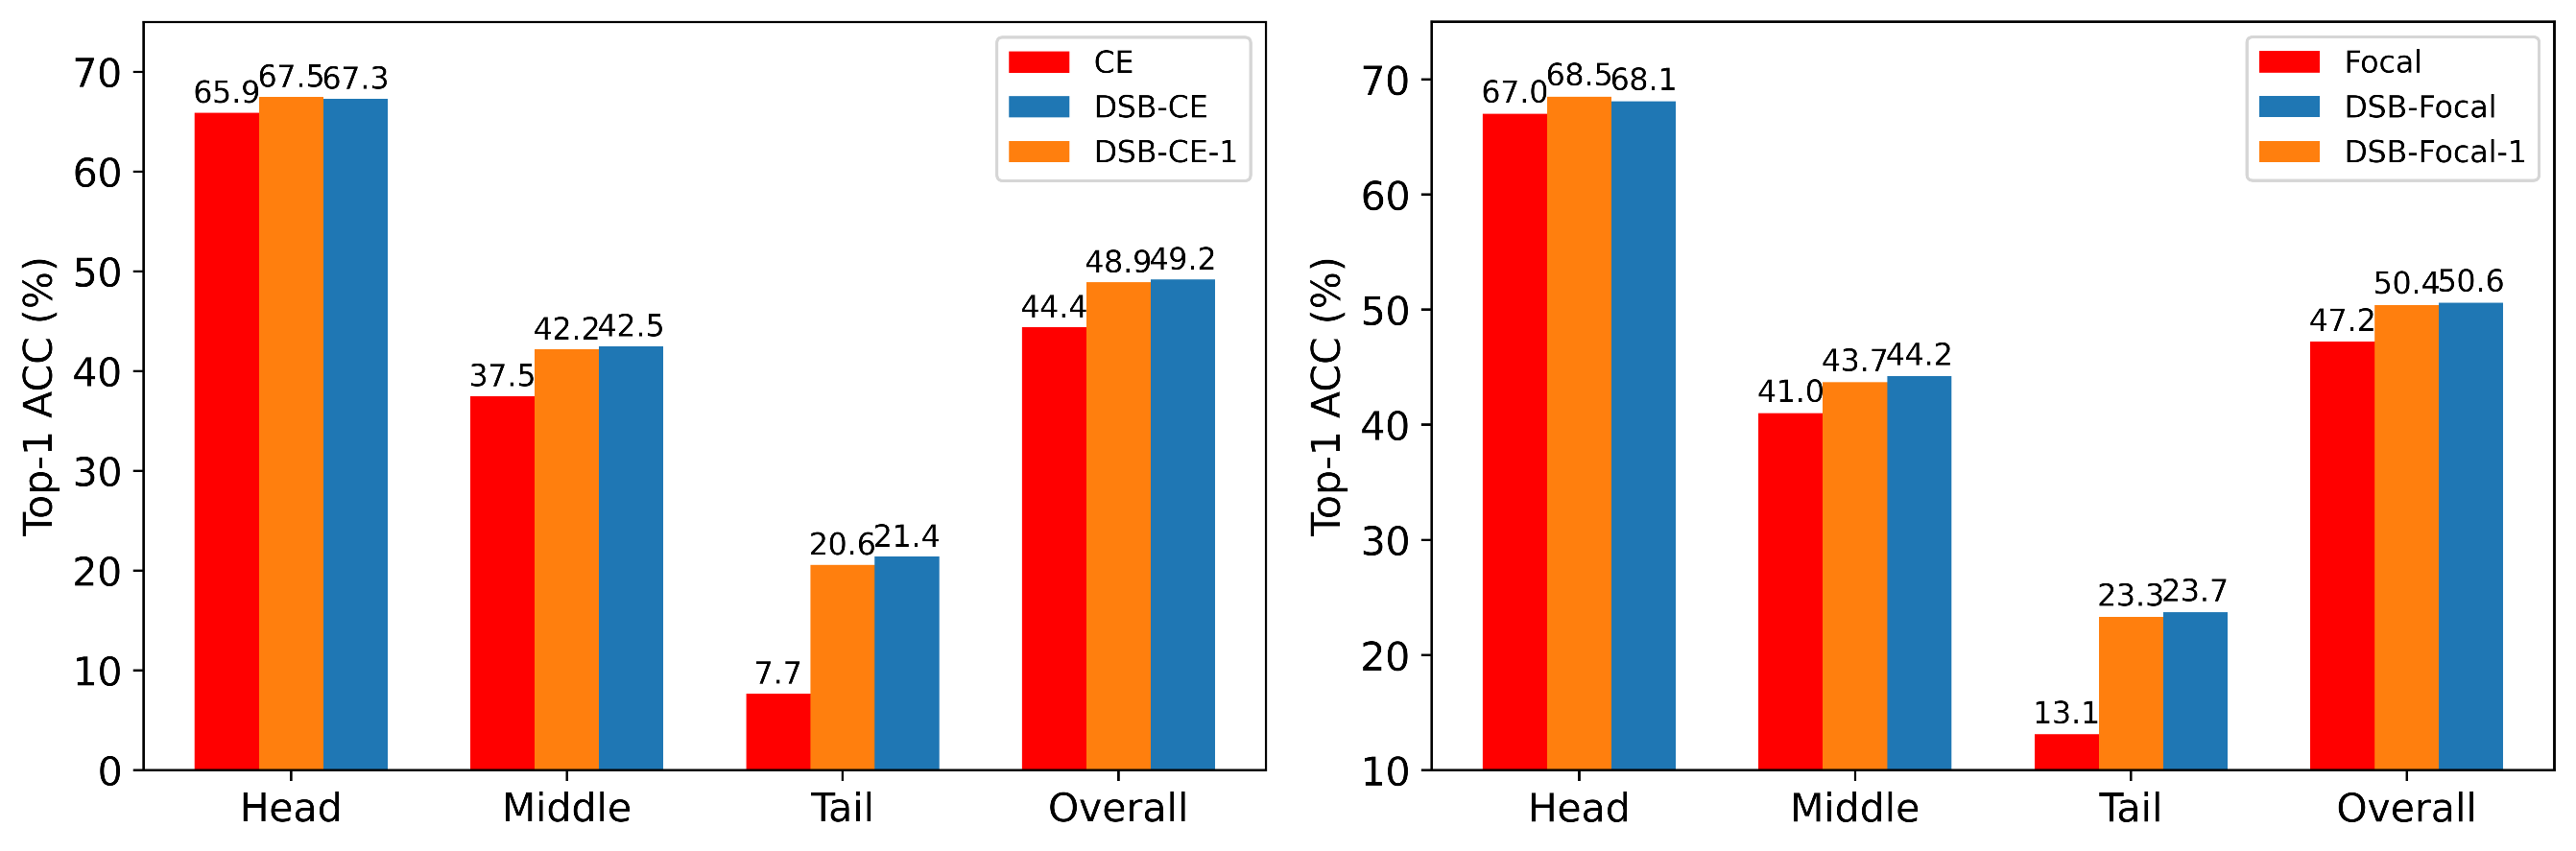
\includegraphics[width=1\columnwidth]{fig21}
\vskip -0.1in
\caption{Accuracy comparison on ImageNet-LT.}
\label{fig21}
\end{center}
\vskip -0.1in
\end{figure*}

The dynamic semantic-scale-balanced loss without considering inter-class interference is denoted as DSB-CE-1 and DSB-Focal-1. The experimental results are shown in Figure \ref{fig21}. It can be observed that DSB-CE-1 and DSB-Focal-1 have almost no performance degradation compared to DSB-CE and DSB-Focal. The above observation is as expected, since our recent study shows that the correlation between the separation degree of feature manifolds and the accuracy of the corresponding class decreases during training and that the existing model can eliminate the main effect of separation degree between feature manifolds on model bias.

%-------------------------------------------------------------------------
\subsection{Comparison with other methods of measuring class-level difficulty\label{H.2}}

Difficult example mining \cite{paper113,paper114} is an instance-level approach, while we focus on class-level difficulty. We note that a recent work on measuring class difficulty (CDB loss \cite{paper27}) was published in IJCV, which can be compared with our work. In addition, LOCE \cite{paper112} and domain balancing \cite{paper111} also measure class-level difficulty, but LOCE is designed for object detection tasks, so we compare semantic-scale-balanced learning with CDB loss and domain balancing. The description of CDB loss, LOCE and domain balancing is as follows.

\begin{itemize}
    \item The imbalance in class performance is referred to as the ``bias'' of the model, and \cite{paper27} defines the model bias as $$bias=\max(\frac{\max_{c=1}^NA_c}{\min_{c'=1}^NA_{c'}+\varepsilon}-1,0),$$ where $A_c$ denotes the accuracy of the $c$-th class. When the accuracy of each class is identical, bias = 0. \cite{paper27} computes the difficulty of class c using $1-A_c$ and calculates the weights of the loss function using a nonlinear function of class difficulty. 
    \item LOCE \cite{paper112} uses the mean classification prediction score to monitor the learning status for different classes and apply it to guide class-level margin adjustment for enhancing tail-class performance \cite{paper2}. 
    \item Domain balancing \cite{paper111} studied a long-tailed domain problem, where a small number of domains (containing multiple classes) frequently appear while other domains exist less. To address this task, this work introduced a novel domain frequency indicator based on the inter-class compactness of features, and uses this indicator to re-margin the feature space of tail domains \cite{paper2}.
\end{itemize}

\begin{figure*}[h] % 纵向8行,图片靠右,宽度12.5em
\begin{center}
\vskip -0.15in
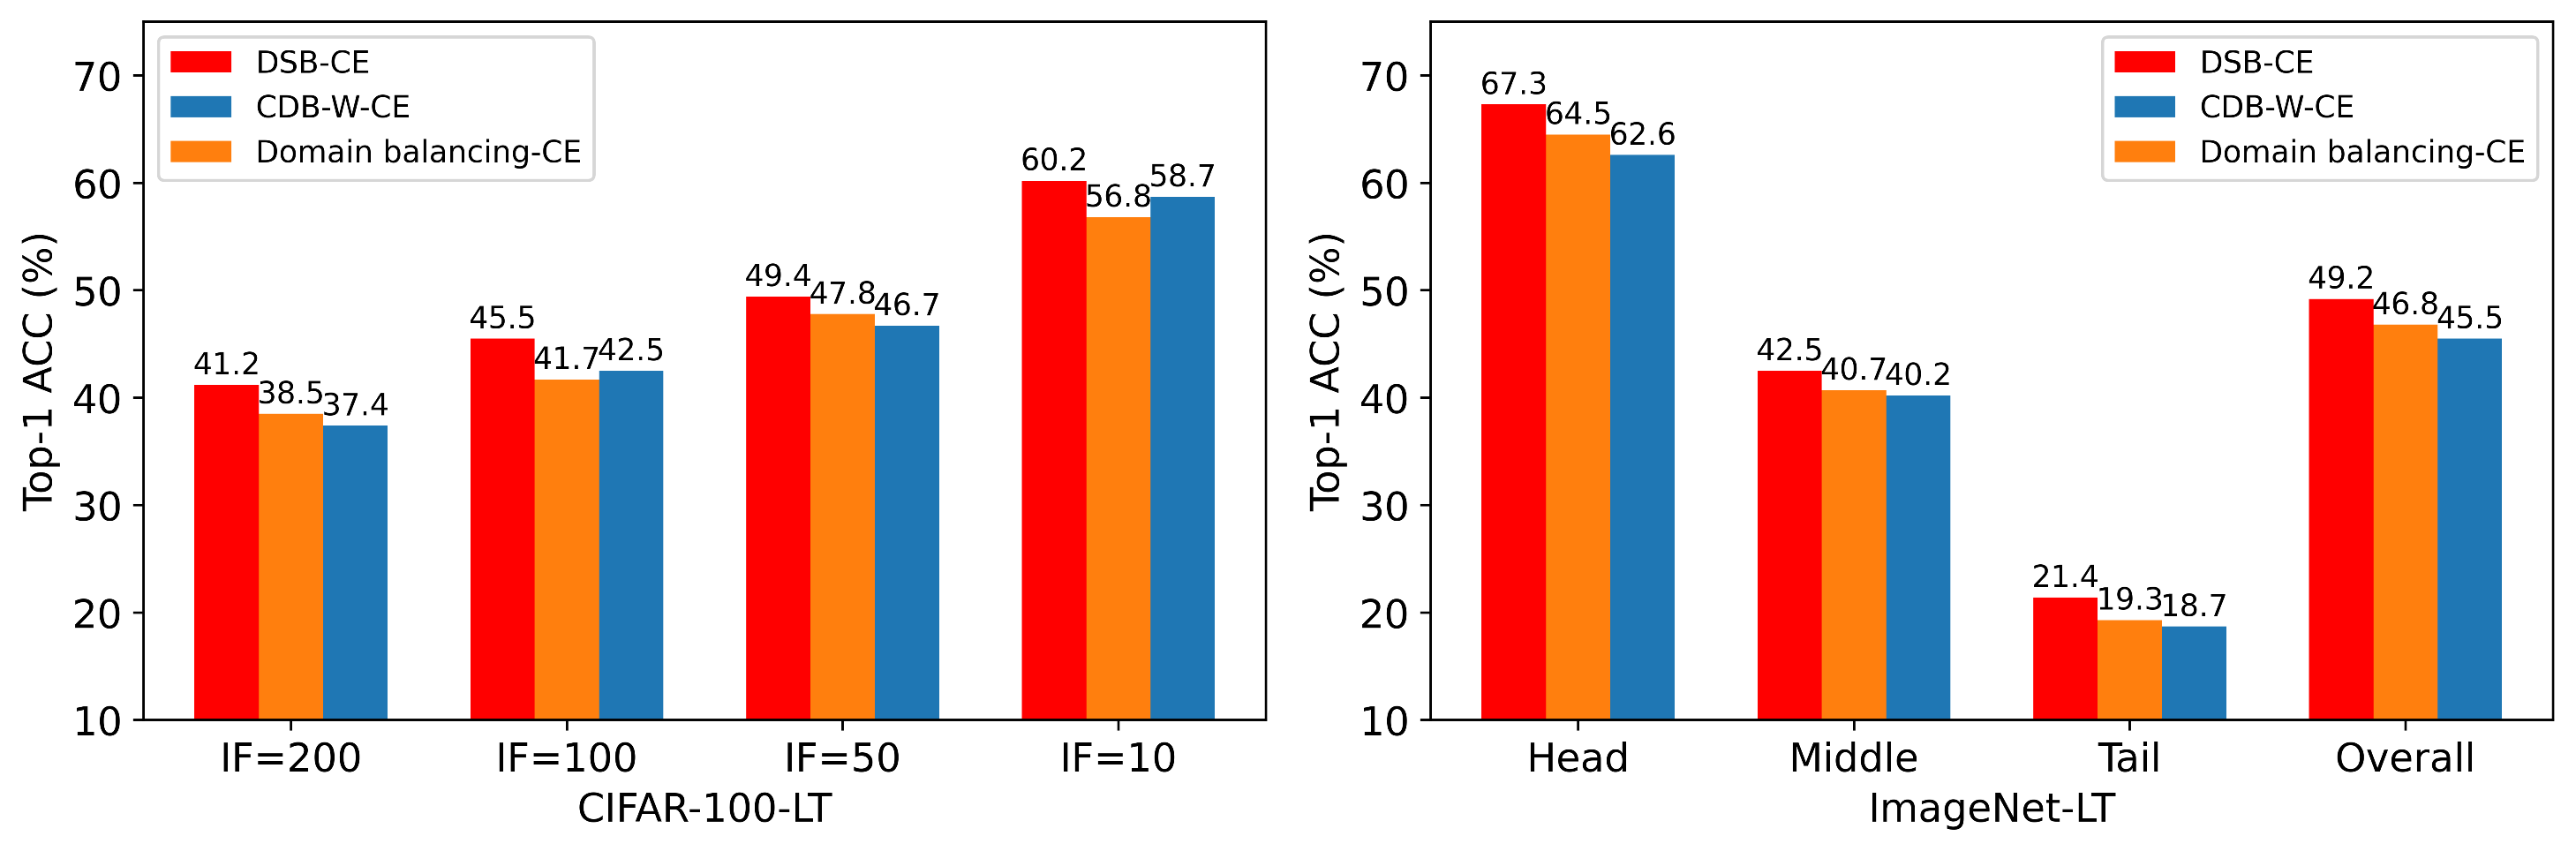
\includegraphics[width=1\columnwidth]{fig22}
\vskip -0.1in
\caption{Accuracy comparison with other methods of measuring class-level difficulty.}
\label{fig22}
\end{center}
\vskip -0.05in
\end{figure*}

We implemented CDB loss \cite{paper27}, LOCE \cite{paper112}, and domain balancing \cite{paper111} on ImageNet-LT. Observing Figure \ref{fig22}, our proposed semantic scale balanced learning outperforms these three approaches. In addition to the comparison with the class-level difficulty weighting method, we add the results of the improvements to PaCO \cite{paper73} in Table \ref{table2}. Balanced softmax is included in PaCO, and although we have shown in Table \ref{table2} that our method significantly improves Balanced softmax, we still improved PaCO and conducted experiments to allay researchers' concerns. All experiments adopted the same training strategy and parameters as in Table \ref{table2}.

\iffalse
\subsection{The performance of dynamic semantic-scale-balanced learning in generalized long-tailed learning\label{H.3}}

Invariant feature learning (IFL \cite{paper115}) considers both inter-class long tail and intra-class long tail and further defines the \textbf{generalized long-tailed classification}. The intra-class long tail has not been considered before, and invariant feature learning takes it into account in the long-tailed classification problem for the first time, which is remarkable progress in solving the long-tailed problem. IFL decomposes the probabilistic model of the classification problem as $P(y\mid x)=\frac{P(x\mid y)}{P(x)}P(y) $ and defaults the class with few samples to be the weak class. \textbf{It should be noted} that our study found that the geometric properties of the manifolds corresponding to different class distributions $P(x)$ will affect the classification difficulty, which breaks the previous perception, so the inter-class long-tail problem still has huge research potential. The existence of data manifolds is already a consensus, and data classification can be regarded as the unwinding and separation of manifolds. Typically, a deep neural network consists of a feature extractor and a classifier. Feature learning can be considered as manifold unwinding, and a well-learned feature extractor is often able to unwind multiple manifolds for the classifier to decode. In this view, all factors about the manifold complexity may affect the model's classification performance. Therefore, we suggest that future work can explore the inter-class long-tailed problem from a geometric perspective. \textbf{Also, both the inter-class long tail and the intra-class long tail need to be considered, which will greatly alleviate the long-tailed problem}.

Invariant feature learning estimates relatively unbiased feature centers by constructing the resampling strategy and uses center loss for unbiased feature learning. We applied IFL to dynamic semantic-scale-balanced learning to consider both the inter-class long tail and the intra-class long tail, and validated it on ImageNet-LT and iNaturalist2018. Experiments show that DSB-CE combined with IFL achieves further performance improvement, and we have supplemented the results and analysis in Table \ref{table2}.


\begin{table*}[h]
\vskip -0.2in
\renewcommand\arraystretch{1.2}
\setlength{\tabcolsep}{13pt} %修改行距
\caption{Evaluation on MSCOCO-GLT.}
\label{table11}
\vskip 0.1in
\centering   
\begin{tabular}{c| c |c |c |c}
\hline
\hline
\multicolumn{2}{c|}{Protocols} & CLT & GLT & ALT \\ 
\hline
\multicolumn{2}{c|}{\textbf{$<$ Accuracy $\vert$ Precision $>$}} & Overall & Overall & Overall \\ 
\hline \toprule 
\multirow{13}{*}{{\rotatebox{90}{\small{\textbf{Re-balance}}}}} 


&cRT~\cite{paper116} &  73.64 $\vert$ 75.84 & 64.69 $\vert$ 68.33 & 49.97 $\vert$ 50.37 \\

&LWS~\cite{paper116} &  72.60 $\vert$ 75.66 & 63.60 $\vert$ 68.81 & 50.14 $\vert$ 50.61 \\

&Deconfound-TDE~\cite{paper117} & 73.79 $\vert$ 74.90 & 66.07 $\vert$ 68.20 & 50.76 $\vert$ 51.68 \\

&BLSoftmax~\cite{paper105} & 72.64 $\vert$ 75.25 & 64.07 $\vert$ 68.59 & 49.72 $\vert$ 50.65 \\

&BBN~\cite{paper10} &  73.69 $\vert$ 77.35 & 64.48 $\vert$ 70.20 & 51.83 $\vert$ 51.77 \\

&LDAM~\cite{paper104} & 75.57 $\vert$ 77.70 & 67.26 $\vert$ 70.70 & 55.52 $\vert$ 56.21 \\ 

&DSB-LDAM &  76.63 $\vert$ 78.95 & 68.15 $\vert$ 71.87 & 56.16 $\vert$ 56.87 \\  \cline{2-5}

&BLSoftmax + IFL \cite{paper115} &  73.72 $\vert$ 77.08 & 64.76 $\vert$ 70.00 & 52.97 $\vert$ 53.52\\  

&DSB-BLSoftmax &  73.96 $\vert$ 77.37 & 65.03 $\vert$ 70.15 & 50.24 $\vert$ 51.36\\  

&DSB-BLSoftmax + IFL &  74.64 $\vert$ 78.06 & 65.47 $\vert$ 70.83 & 53.08 $\vert$ 53.75\\  \cline{2-5}


&cRT + IFL \cite{paper115} &  76.21 $\vert$ 79.11 & 66.90 $\vert$ 71.34 & 52.07 $\vert$ 52.85\\  

&DSB-cRT &  \textbf{76.82} $\vert$ \textbf{79.95} & \textbf{67.26} $\vert$ \textbf{71.73} & 51.41 $\vert$ 51.94\\  \cline{2-5}


&LWS + IFL \cite{paper115} &  75.98 $\vert$ 79.18 & 66.55 $\vert$ 71.49 & 52.07 $\vert$ 52.90\\  

&DSB-LWS &  \textbf{76.55} $\vert$ \textbf{80.06} & \textbf{67.03} $\vert$ \textbf{72.15} & 51.64 $\vert$ 51.16\\  


 \bottomrule \hline
\end{tabular}
%\vskip -0.1in
\end{table*}

We note that IFL proposes two datasets ImageNet-GLT and MSCOCO-GLT and three testing protocols. Since our paper already contains a large number of experiments, we selected to conduct experiments on MSCOCO-GLT with the same experimental settings as IFL. The results are shown in Table \ref{table11}. On the CLT and GLT protocols, we significantly improve the performance of BL-softmax, LDAM, and BL-softmax+IFL. Also, our approach promotes the performance of the above three methods on the ALT protocol, which may be caused by the additional gain from stronger inter-class discriminability. Due to page limitations, the experiment is tentatively supplemented in the appendix, and we will include this experiment in the main text if the paper is accepted. The experiments show that alleviating both inter-class long tail and intra-class long tail can significantly improve the model performance, so \textbf{we encourage researchers to pay attention to the intra-class long-tailed problem}.
\fi

\subsection{Performance of Dynamic Semantic-Scale-Balanced Learning on Three Subsets of ImageNet\label{H.4}}

We divided ImageNet into Head, Middle, and Tail subsets based on semantic scale, which contain $333$, $333$, and $334$ classes, respectively. The performance of DSB-CE and CE on the three subsets when the backbone networks are VGG-16 and ResNet-18 is shown in Figure \ref{fig23}.

The experimental results show that semantic-scale-balanced learning significantly improves the performance of CE on Tail subset. Meanwhile, DSB-CE also outperforms CE on Head and Middle, which may be caused by the performance gain from better feature learning. In addition to the classification problem, we hope to introduce semantic scale imbalance in the fields of object detection, semantic segmentation, etc. to promote the fairness of the model.

\begin{figure*}[h] % 纵向8行,图片靠右,宽度12.5em
\begin{center}
%\vskip -0.01in
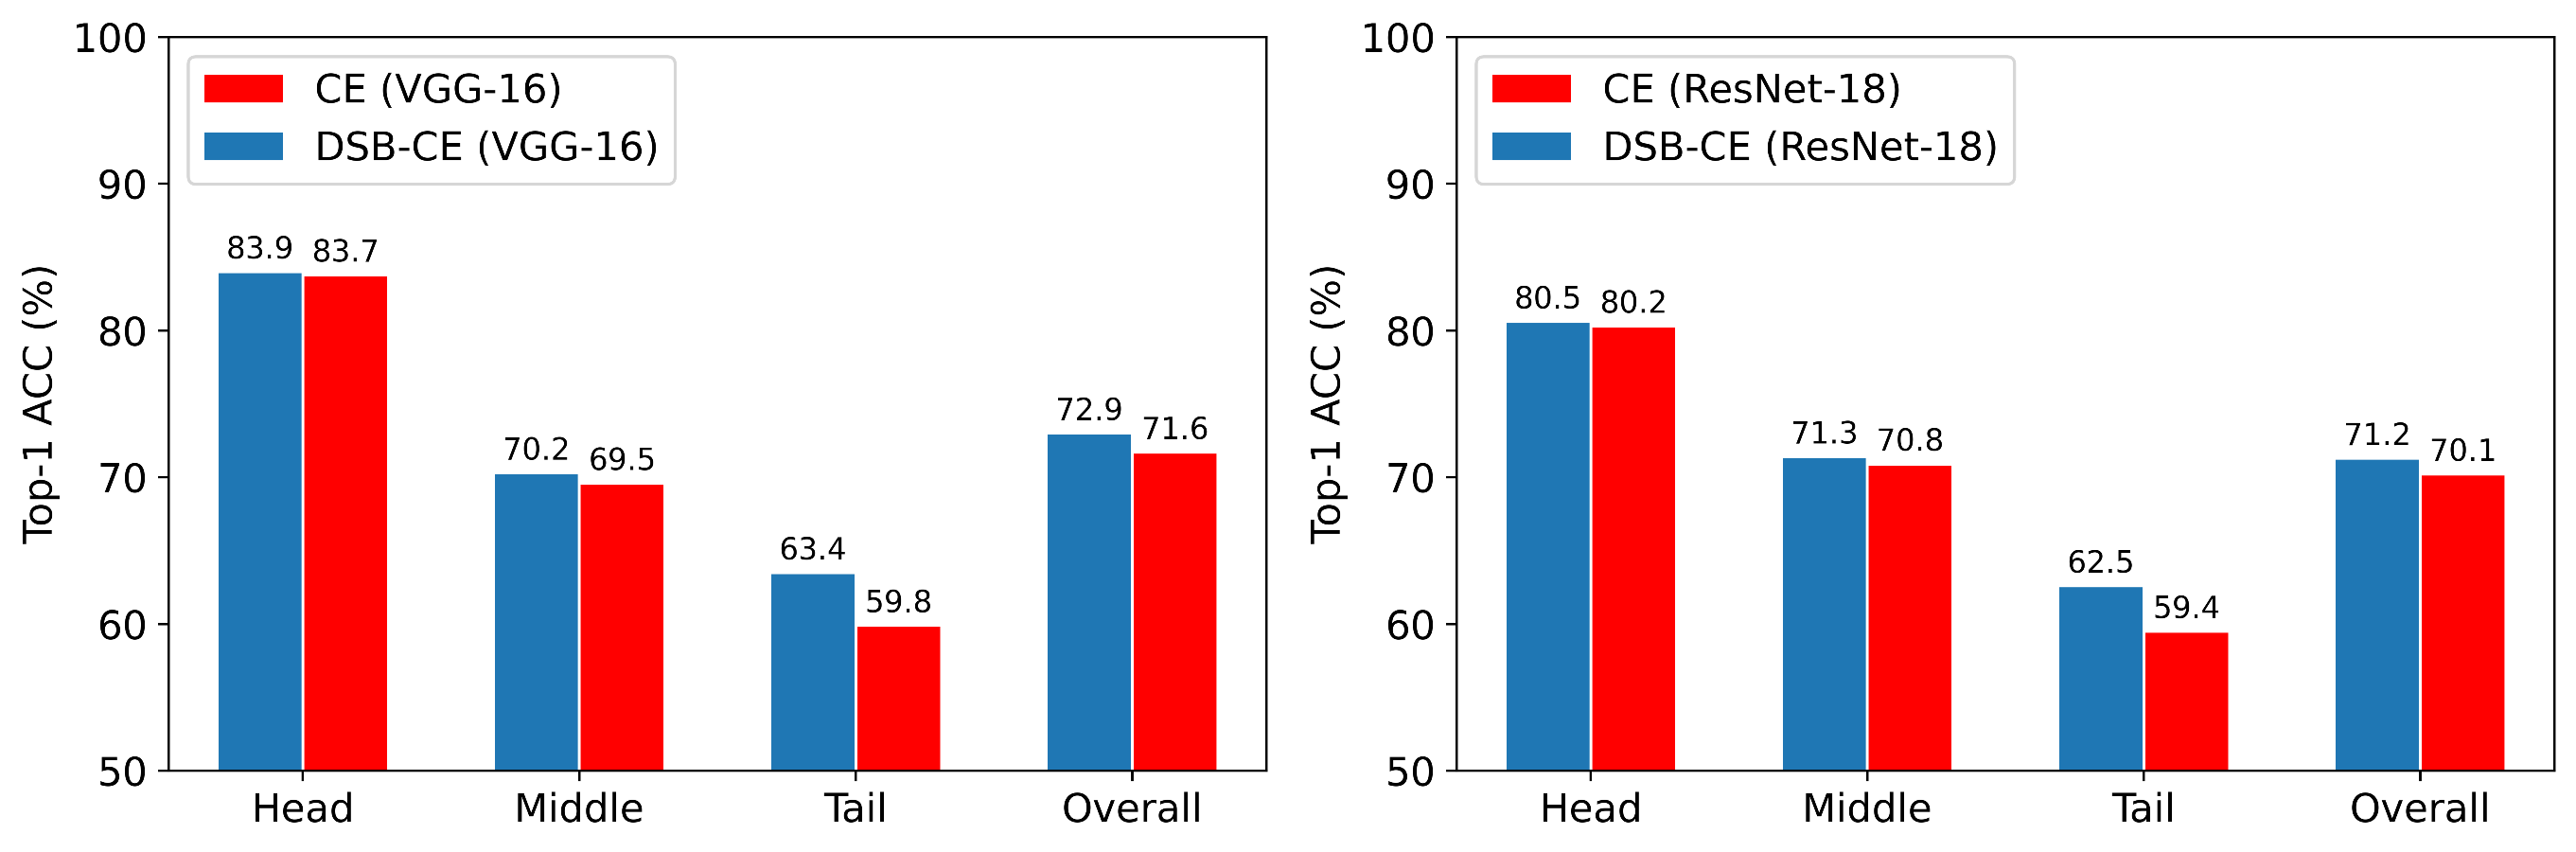
\includegraphics[width=1\columnwidth]{fig23}
\vskip -0.1in
\caption{Comparison of CE and DSB-CE on ImageNet, where the backbone networks are VGG-16 and ResNet-34, respectively. It can be observed that dynamic semantic-scale-balanced learning significantly improves the tail class performance.}
\label{fig23}
\end{center}
\vskip -0.2in
\end{figure*}

\section{Apply Semantic Scale to Solve Other Problems\label{I}}
\subsection{Select Well-Represented Data\label{I.1}}

Downsampling the head class is one of the methods to alleviate the long tail problem, which balances the number of samples but leads to the loss of head class information. Therefore, it is important to develop a downsampling method that preserves the head information. We propose an idea to select well-represented data based on the geometric meaning of semantic scale.

The existence of data manifolds is a consensus that the same class of data is usually distributed around a low-dimensional manifold. Different dimensions of the manifold represent different physical characteristics, and samples located at the edges of the manifold often tend to overlap with other manifolds. Therefore, we believe that the following two principles should be obeyed when downsampling:

\begin{itemize}
     \item Uniform sampling inside the manifold. It ensures that the volume of the manifold does not shrink significantly after downsampling.
     \item Increase the sampling rate of samples at the edges of the manifold. It makes the sampled distribution with significant bounds, which helps to improve the robustness of the classification model.
\end{itemize}

As shown in Figure \ref{fig24}, we refer to the strategy that obeys the above sampling principles as \textbf{"pizza" sampling}.

\begin{figure*}[h] % 纵向8行,图片靠右,宽度12.5em
\begin{center}
%\vskip -0.01in
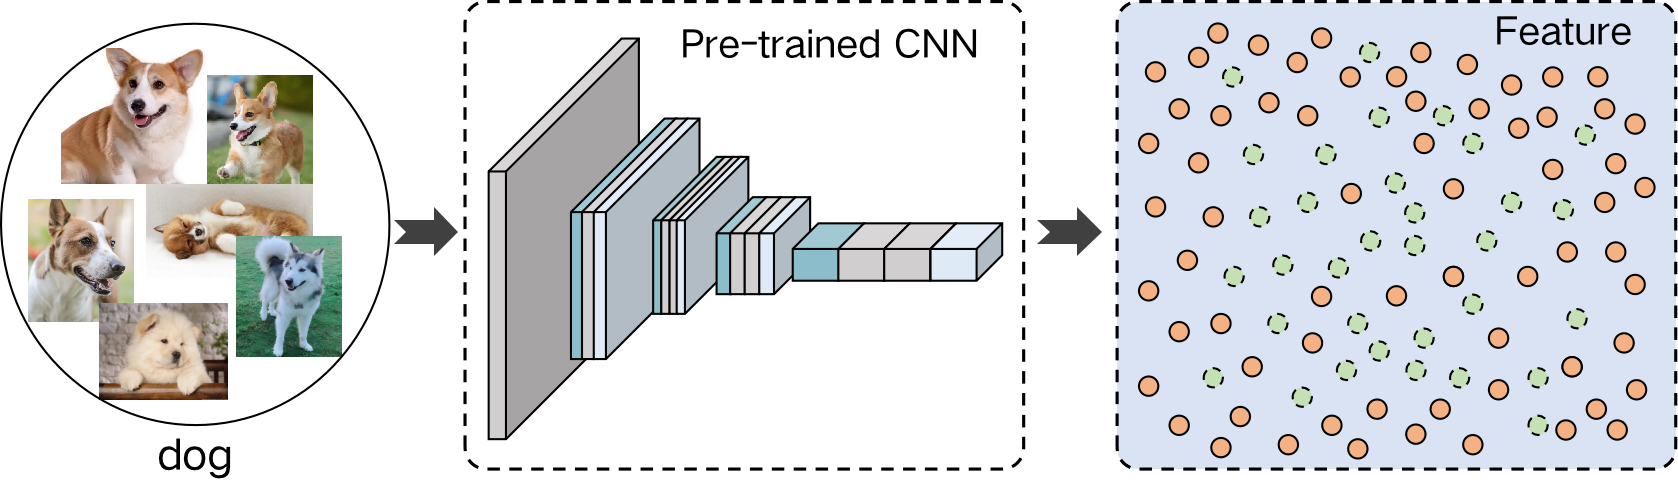
\includegraphics[width=1\columnwidth]{fig34}
\vskip -0.05in
\caption{Schematic diagram of pizza sampling. Yellow samples indicate the selected samples and green samples indicate the discarded samples.}
\label{fig24}
\end{center}
\vskip -0.05in
\end{figure*}

Uniform sampling is easy to do, but how do we sample as many samples as possible from the edges of the manifold? We propose to randomly sample $k$ subsets in the original sample set and calculate the semantic scales of the subsets. Then repeat the above operation several times and select the subsets with the largest semantic scales as the final samples.


\subsection{Guide Data Collection\label{I.2}}

When collecting data that has never been studied before, we do not know how many samples to collect to represent their corresponding class well because of the lack of prior knowledge. When too few samples are collected, the class is under-represented. And sampling too many samples will consume huge costs. The marginal effect of the semantic scale can help us judge whether the currently collected samples have enough feature diversity, and we can stop collecting samples when the feature diversity tends to be saturated. Specifically, the data collection process is as follows.

\begin{itemize}
     \item[(1)] For class $c$, $m$ samples are collected each time.
     \item[(2)] After the $(n-1)$th collection of samples, there are $(n-1)\times m$ samples, and the semantic scales of these samples are calculated.
     \item[(3)] After the $n$th collection of samples, there are $n \times m$ samples, and the semantic scales of these samples are calculated.
     \item[(4)] Calculate the increment of the semantic scale for the $n$th time relative to the $(n-1)$th time.
     \item[(5)] Calculate $\frac{(S_n-S_{n-1})}{S_n}$. If the increment of semantic scale is less than $\alpha\%$ of $S_n$, it means that the feature diversity of class $c$ has not changed significantly and the sample collection can be stopped. The parameter $\alpha$ can be adjusted according to the needs of the task.
\end{itemize}

Geometric analysis of data manifolds can bring new perspectives to data science. We will open source the toolkit for measuring the information geometry of data, which includes the application of semantic scale in various scenarios, such as data collection, and representative data selection.

\iffalse
\section{Future Work\label{J}}

\subsection{Model-Independent Measure of Data Difficulty\label{J.1}}

The performance of the models varies across classes. In the past, it was believed that model bias was caused by an imbalance in sample numbers, but a growing body of research suggests that sample numbers are not the only factor affecting model bias. Of course, model bias is also introduced not by the model structure, but by the characteristics of the data itself that affect model performance. Therefore, it is very important to propose model-independent measurements to represent the data itself, and this work will greatly contribute to our understanding of deep neural networks. In this paper, the effect of the volume of the data manifold on the model bias is explored from a geometric perspective. It provides a new direction for future work, namely the geometric analysis of deep neural networks. The geometric characteristics of the data manifold will help us further reveal how neural networks learn and inspire the design of neural network structures.

\begin{figure*}[h]% 纵向8行,图片靠右,宽度12.5em
\begin{center}
%\vskip -0.1in
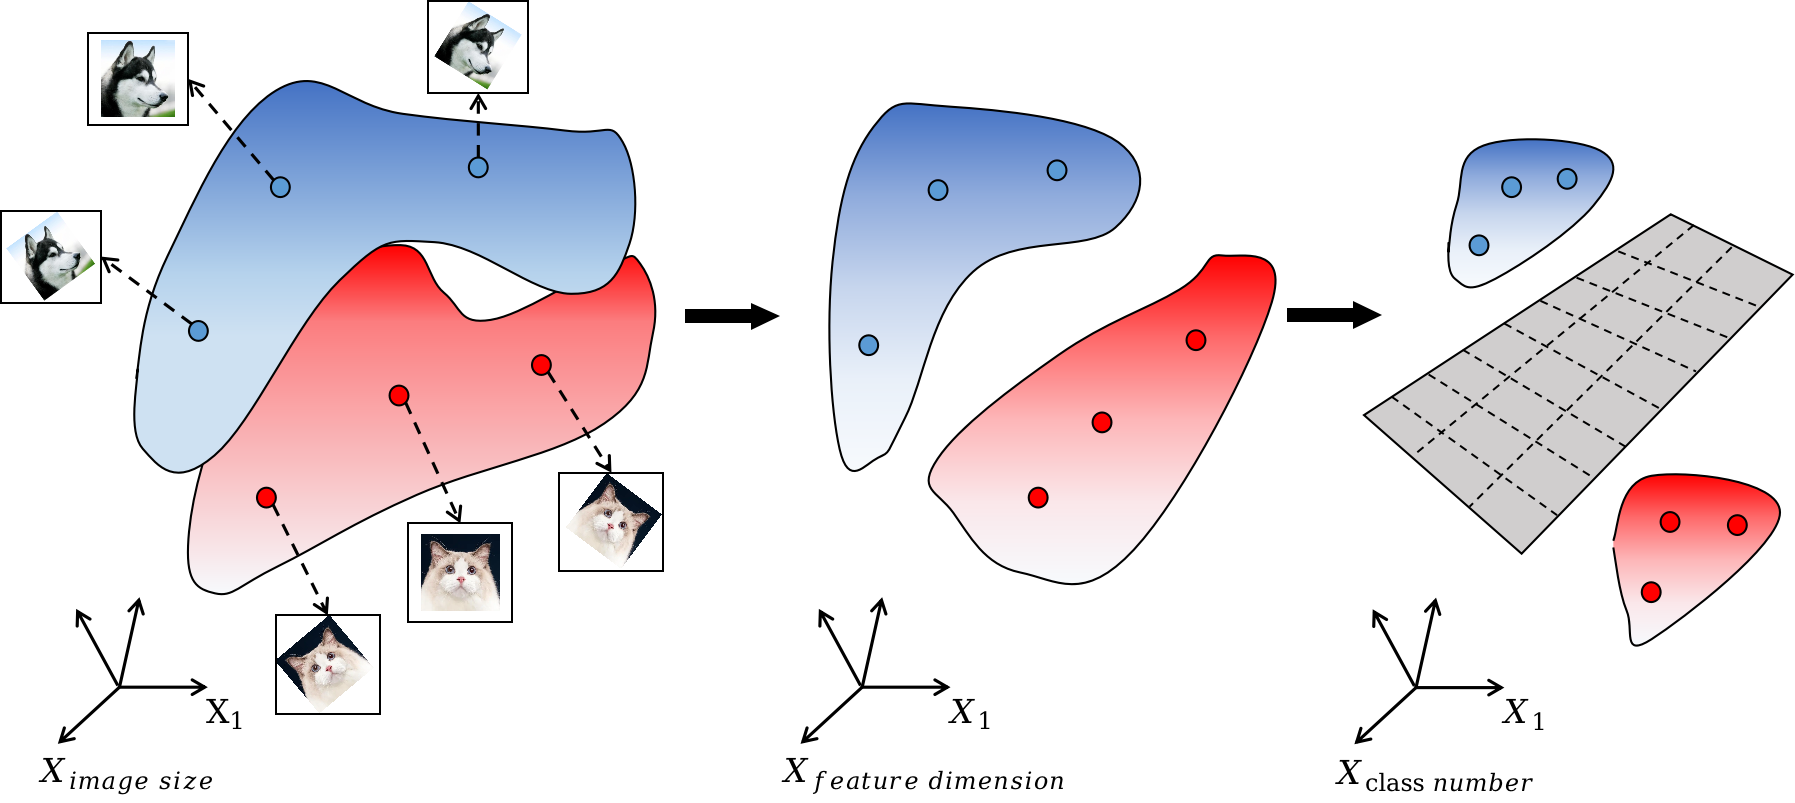
\includegraphics[width=1\columnwidth]{fig24}
\vskip -0.05in
\caption{Changes in the geometry of data manifolds as they are transformed in a deep neural network. The classification process of the data includes untangling the manifolds from each other and separating the different manifolds.}
\label{fig25}
\end{center}
\vskip -0.15in
\end{figure*}

\subsection{A Geometric Perspective on Data Classification\label{J.2}}

Natural datasets have intrinsic patterns that can be generalized to the manifold distribution principle: the distribution of a class of data is close to a low-dimensional manifold. As shown in Figure \ref{fig25}, data classification can be regarded as the unwinding and separation of manifolds. When a data manifold is entangled with other perceptual manifolds, the difficulty of classifying that manifold increases. Typically, a deep neural network consists of a feature extractor and a classifier. Feature learning can be considered as manifold unwinding, and a well-learned feature extractor is often able to unwind multiple manifolds for the classifier to decode. In this view, all factors about the manifold complexity may affect the model's classification performance. Therefore, we suggest that future work can explore the inter-class long-tailed problem from a geometric perspective.


\subsection{Introduce Semantic Scale Imbalance in Object Detection\label{J.3}}

Long-tailed distribution is one of the main difficulties faced by object detection algorithms in real-world scenarios. The classical object detection algorithms are generally trained on some manually designed datasets with relatively balanced data distribution. In contrast, the accuracy of these algorithms tends to suffer significantly on long-tailed distributed datasets. So far, methods for foreground-background imbalance and class imbalance have been proposed extensively, but these methods are based on the number of objects to define the degree of imbalance and cannot explain more phenomena. We will give examples below.

In the field of object detection, it is often encountered that although a class does not appear frequently, the model can always detect such instances efficiently. It is easy to observe that classes with simple patterns are usually easier to learn, even if the frequency of such classes is low. Therefore, classes with low frequency in object detection are not necessarily always harder to learn. We believe that it is a valuable research direction to analyze the richness of the instances contained in each class, and then pay more attention to the hard classes. The dimensionality of all images or feature embeddings in the image classification task is the same, which facilitates the application of the semantic scale proposed in this paper. However, the non-fixed dimensionality of each instance in the field of object detection brings new challenges, so we have to consider the effect of dimensionality on the semantic scale, which is a direction worthy of further study.

\begin{figure*}[t]% 纵向8行,图片靠右,宽度12.5em
\begin{center}
%\vskip -0.32in
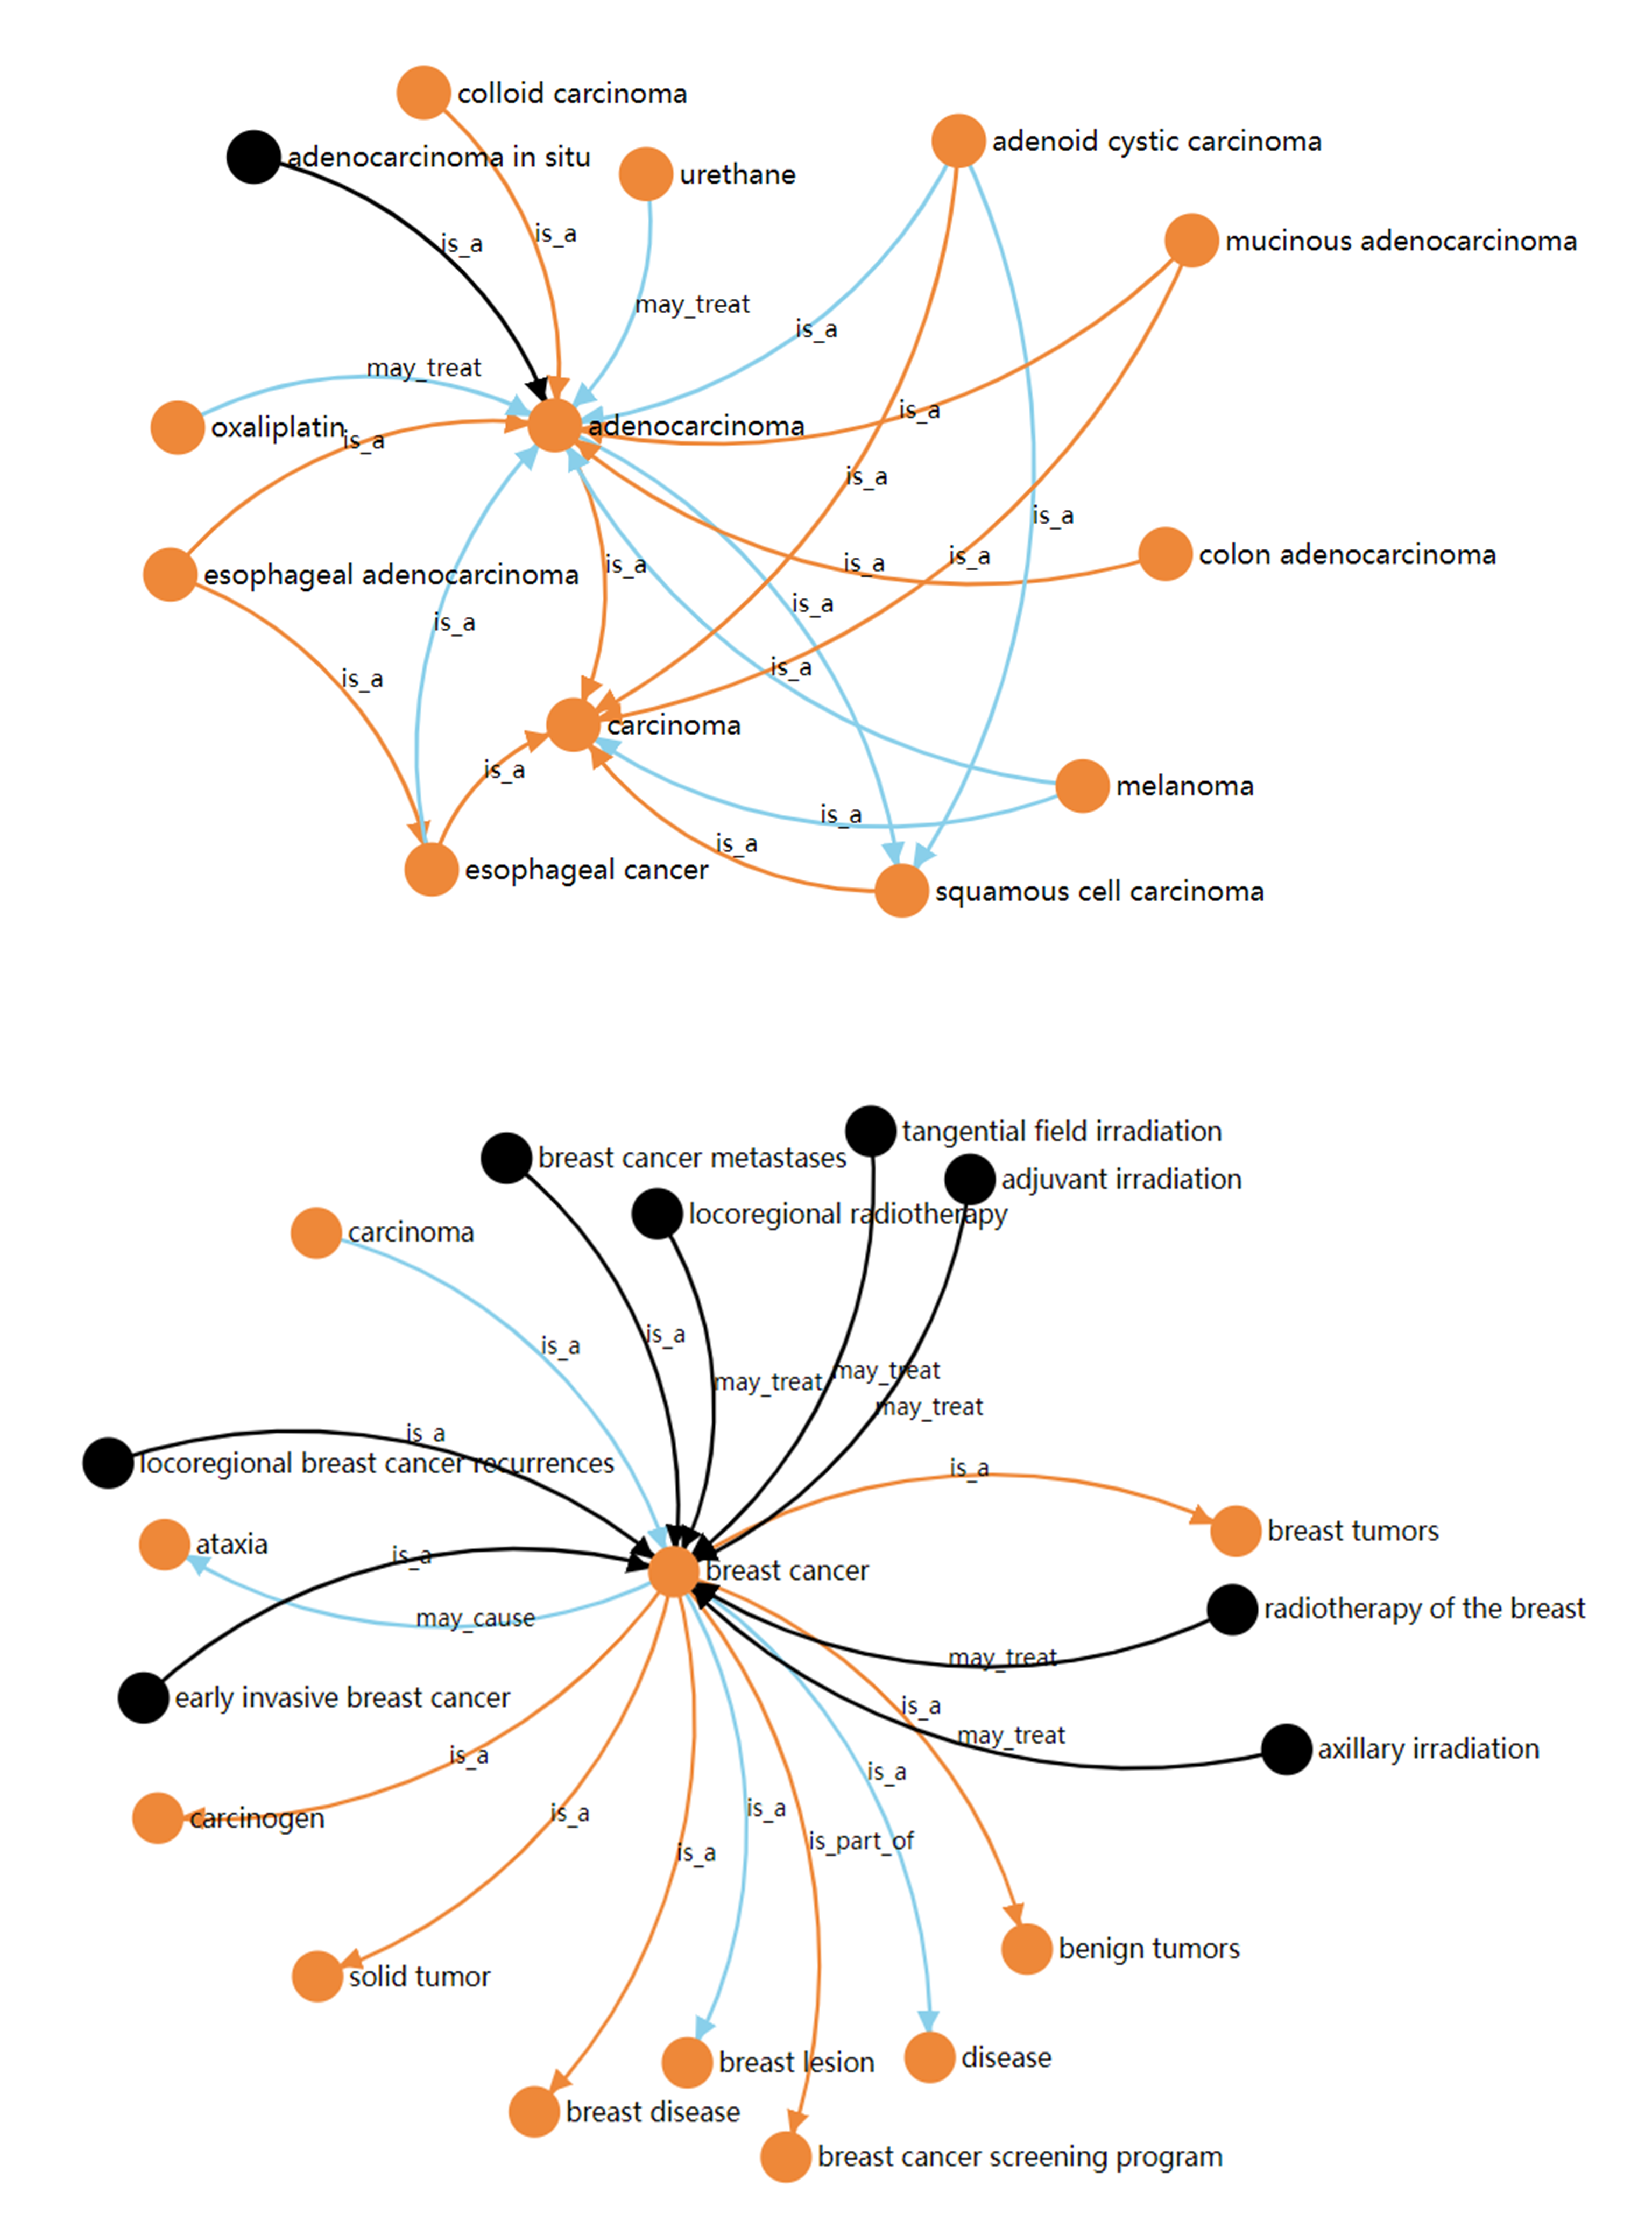
\includegraphics[width=1\columnwidth]{figure2}
\vskip -0.14in
\caption{\textbf{Left column}: curves of semantic scales with increasing number of samples for the first ten classes from different datasets. \textbf{Right column}: for different sub-datasets, curves of the sum of semantic scales for all classes and top-1 accuracy curves of trained ResNet-18 and ResNet-34. All models are trained using the Adam optimizer \cite {paper33} with an initial learning rate of $0.01$ and then decayed by $0.98$ at each epoch.}
\label{fig26}
\end{center}
\vskip -0.1in
\end{figure*}

\fi

\section{More explanation of Figure \ref{fig2}\label{K}}

To see it more clearly, we zoomed in on Figure \ref{fig2} and plotted it in Figure \ref{fig26}. Previous studies have observed that (1) given sufficient data, the classification performance gain is marginal with additional samples. (2) When the data is insufficient, the classification performance drops sharply as the number of training samples decreases. We speculate that phenomenon $1$ may be caused by the marginal effect of feature diversity. It should be noted that CB loss considers marginal effects, but it only qualitatively describes the gradual flattening of feature diversity with the increasing number of samples. Taking CIFAR-10 as an example, we first select a few samples for each class, train the model and test the accuracy. Then new samples are continuously added to the original samples instead of re-selecting more samples to train the model. The experiments corresponding to each point in Figure \ref{fig2} are trained from scratch. While increasing the data we find that there are marginal effects of semantic scale, which indicates that our proposed measurement is as expected. The marginal effects of feature diversity explain phenomenon $1$. 

However, phenomenon $2$ is not explained by the marginal effects, and the effective number of samples from CB loss does not predict phenomenon $2$ at all, because the effective number of samples does not grow faster than the number of samples (which we have analyzed in Section \ref{2}). We experimentally find that when the samples are few, the feature diversity measured by the semantic scale increases rapidly with the number of samples, and this increase is faster than the linear increase. The rapid increase of feature diversity measured by the semantic scale explains phenomenon $2$.
%-------------------------------------------------------------------------

\begin{figure*}[h]% 纵向8行,图片靠右,宽度12.5em
\begin{center}
\vskip -0.05in
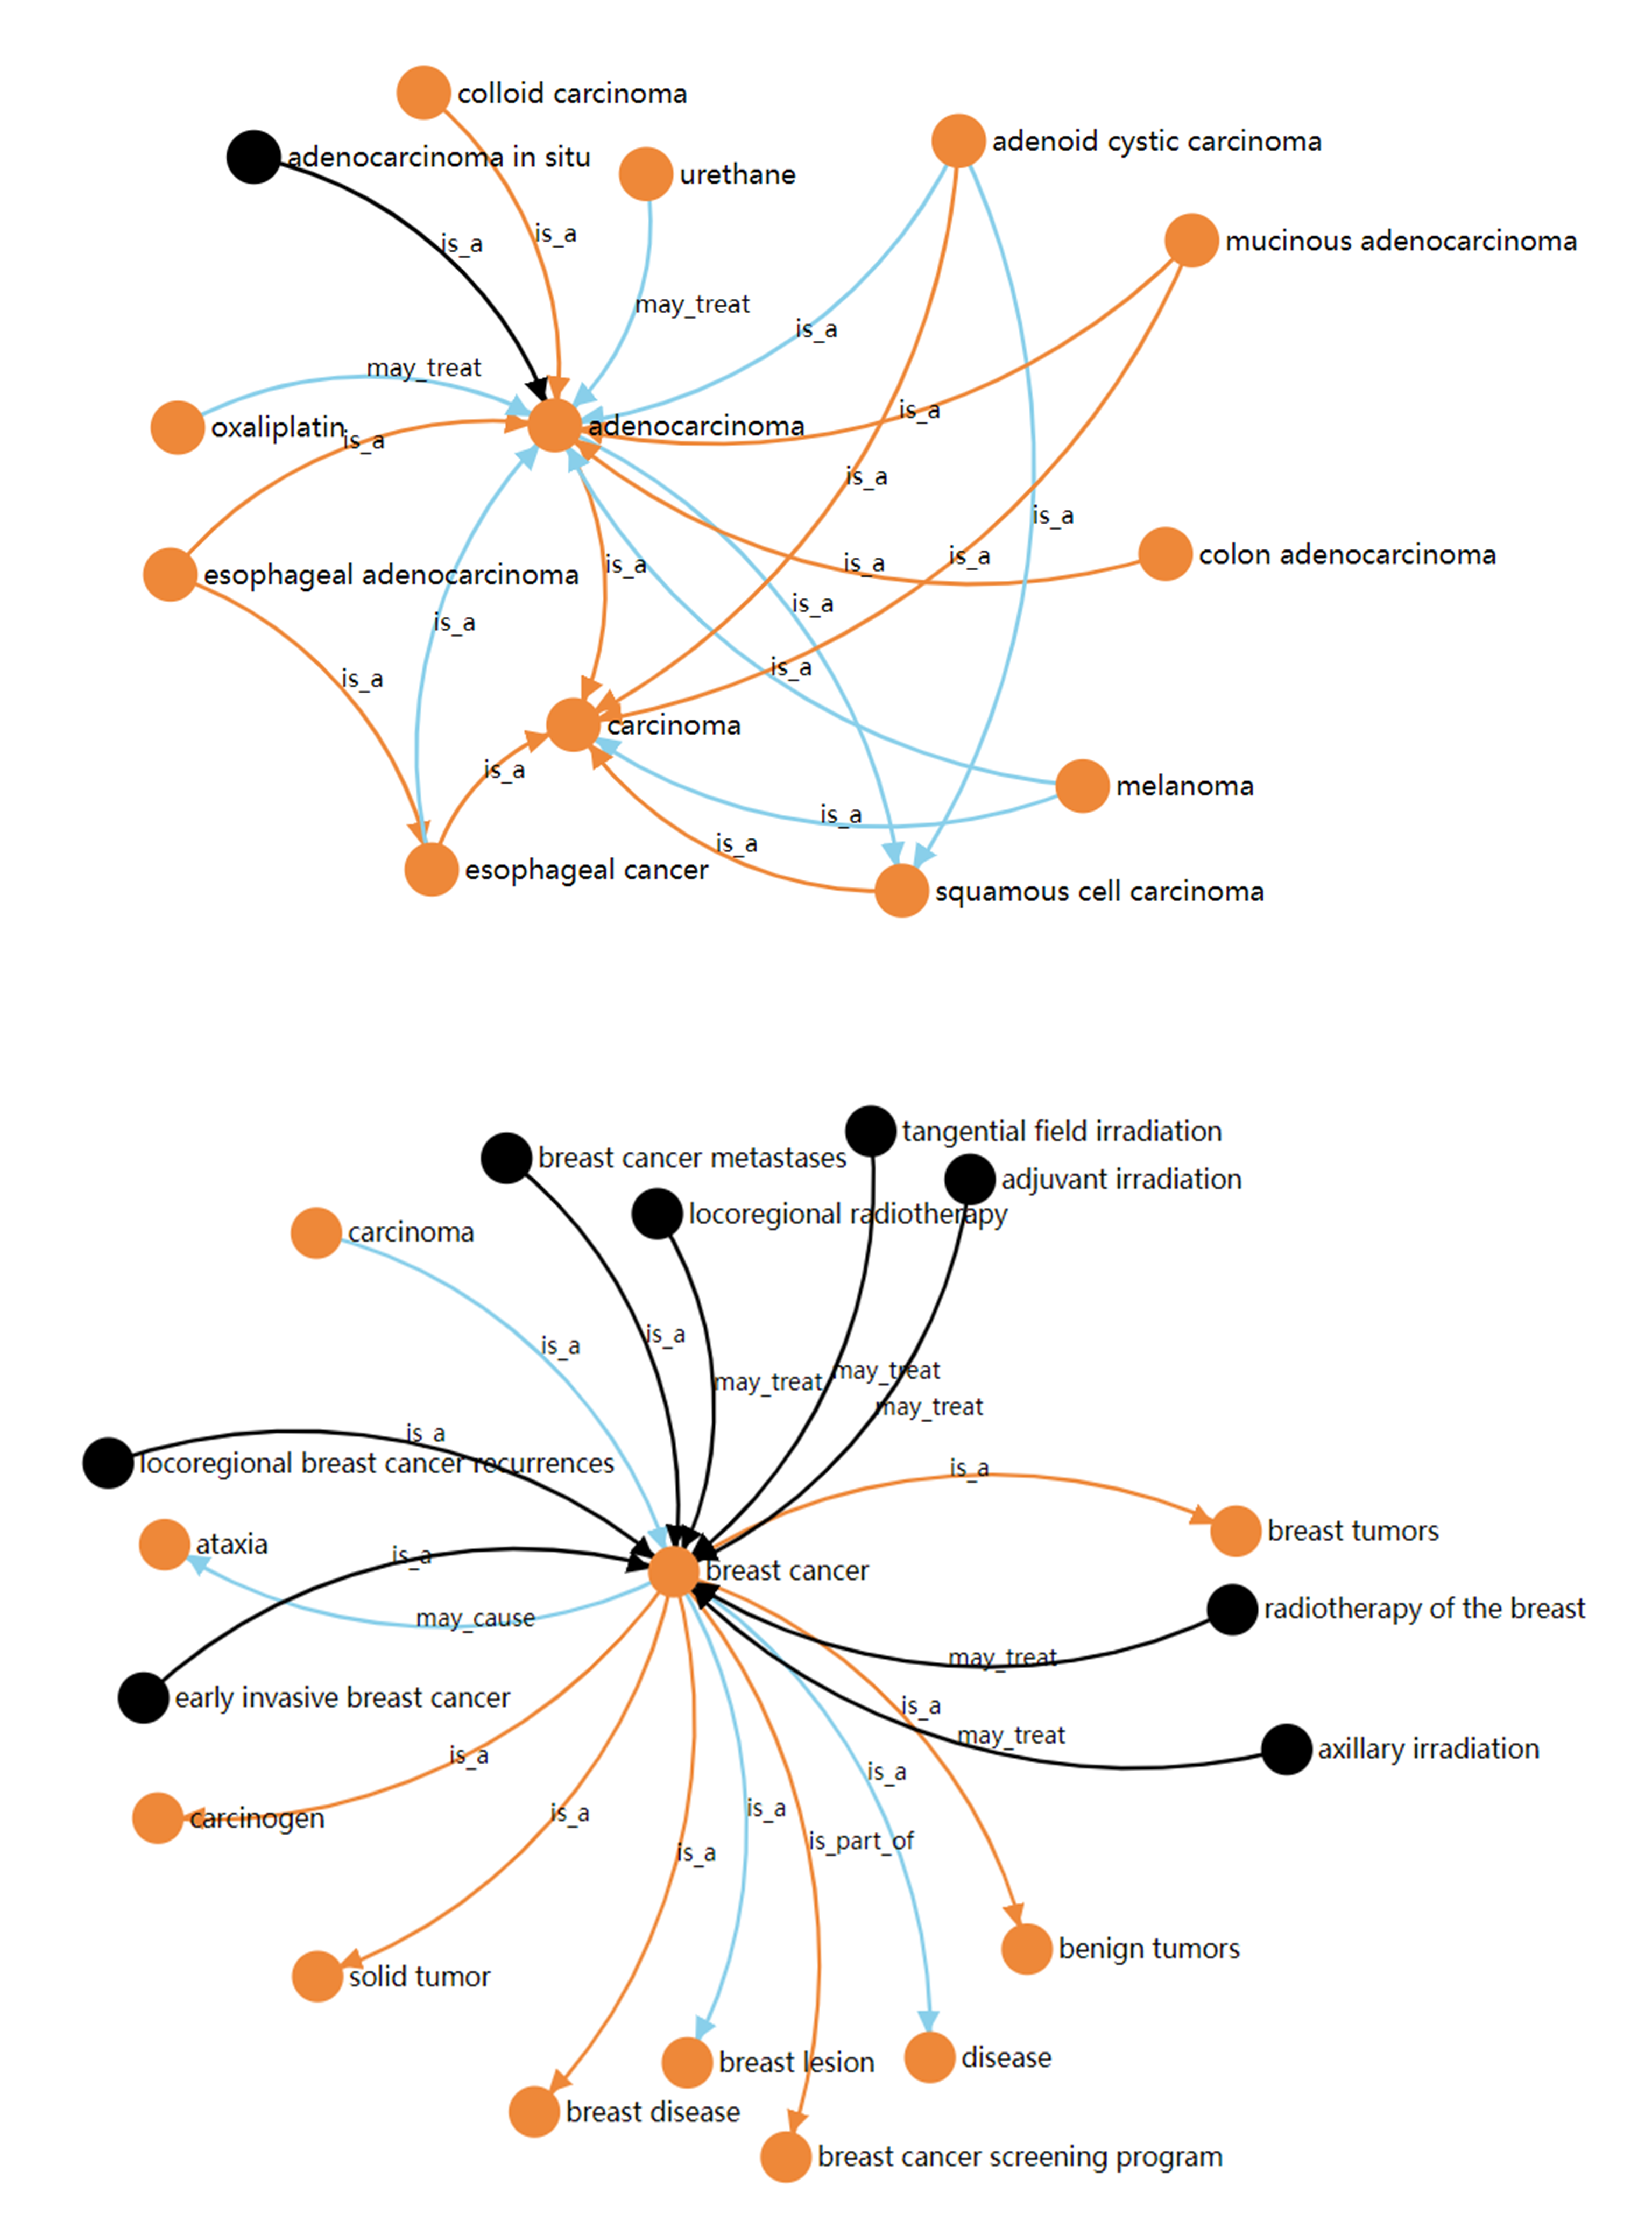
\includegraphics[width=1\columnwidth]{figure2}
\vskip -0.15in
\caption{\textbf{Left column}: curves of semantic scales with increasing number of samples for the first ten classes from different datasets. \textbf{Right column}: for different sub-datasets, curves of the sum of semantic scales for all classes and top-1 accuracy curves of trained ResNet-18 and ResNet-34. All models are trained using the Adam optimizer \cite {paper33} with an initial learning rate of $0.01$ and then decayed by $0.98$ at each epoch.}
\label{fig26}
\end{center}
\vskip -0.3in
\end{figure*}

\section{Can the semantic scale capture the hierarchical structure?\label{L}}

HCSC \cite{paper118} constructs the hierarchical structure of classes by bottom-up k-means, and we use the example shown by HCSC to validate our approach. Given the following seven classes: Poodles, Samoyeds, Labradors, Persian, Siamese, Chimpanzee, and Gorilla, each class contains $1,000$ samples, and the hierarchical structure of the seven classes is shown in Figure \ref{fig27}.

\begin{figure*}[h]% 纵向8行,图片靠右,宽度12.5em
\begin{center}
%\vskip -0.32in
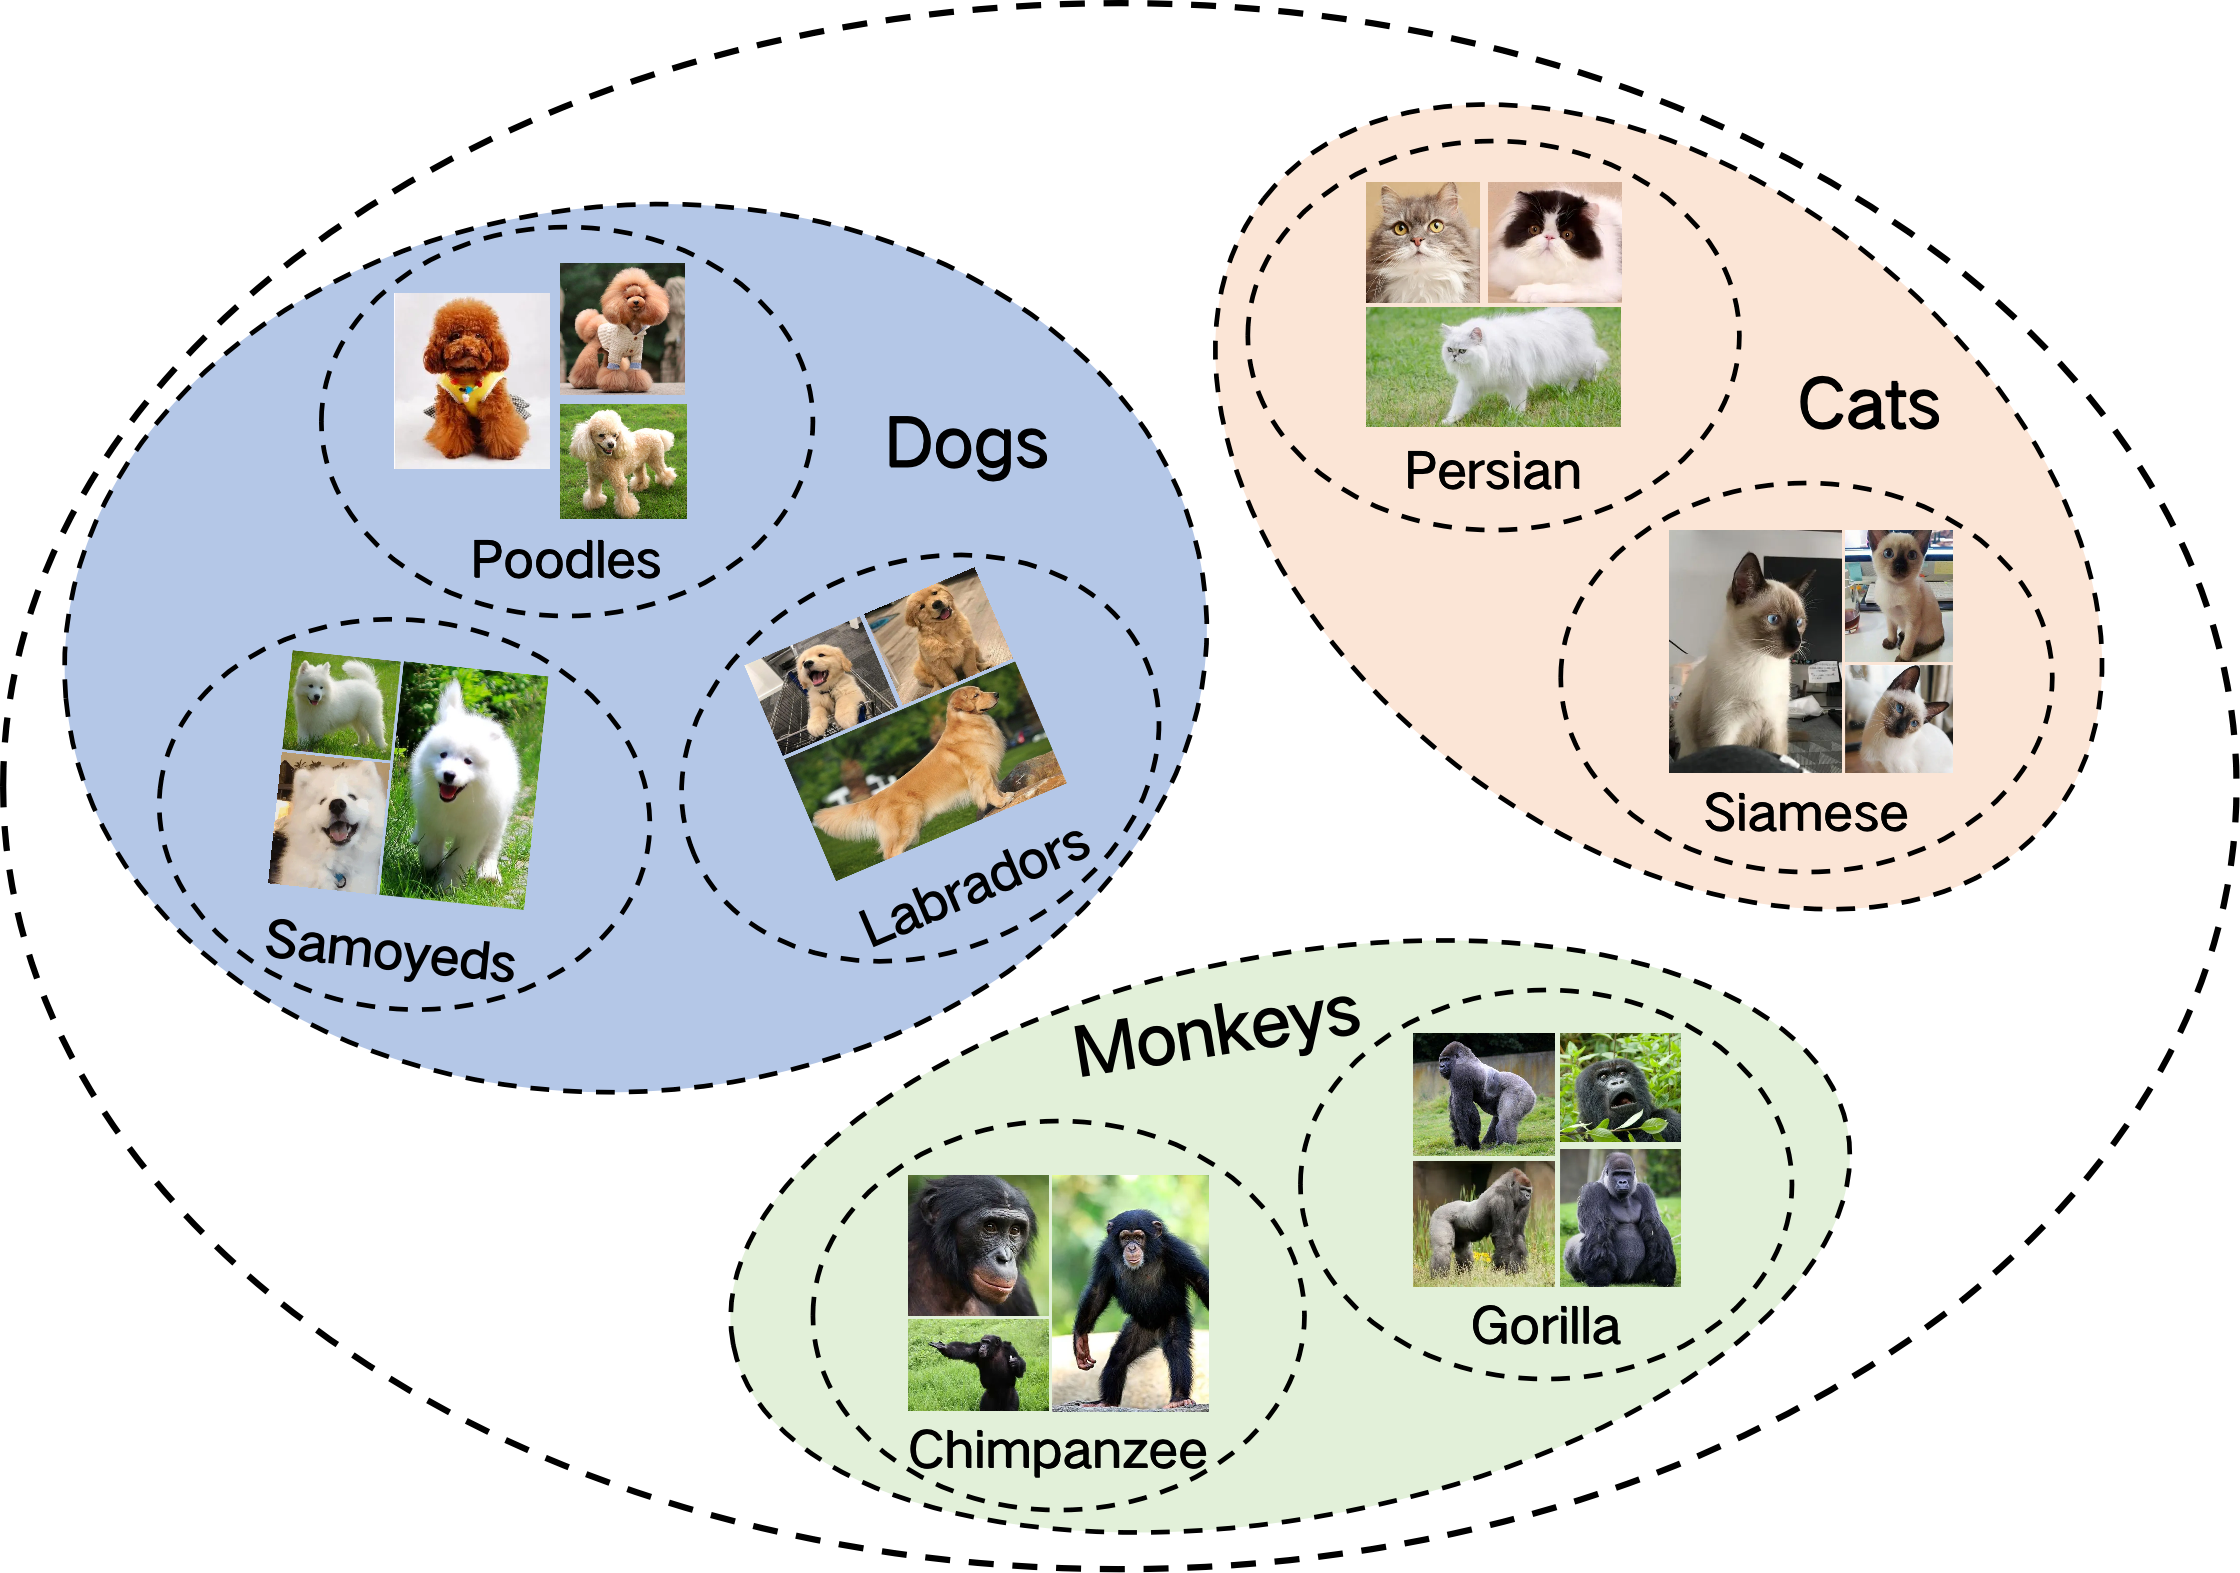
\includegraphics[width=0.65\columnwidth]{fig25}
\vskip -0.05in
\caption{Image datasets typically contain multiple semantic hierarchies.}
\label{fig27}
\end{center}
\vskip -0.14in
\end{figure*}


\begin{table}[h]
%\vskip -0.15in
\renewcommand\arraystretch{1.6}
\setlength{\tabcolsep}{5pt} %修改行距
\caption{\textbf{Results of matching parent class for each child class}, where the Ratio of semantic scales denotes the ratio of the semantic scales of the parent class after mixing to before mixing, Predicted parent class means the parent class we matched for the child class, and Real parent class denotes the real parent class corresponding to the child class.}
\label{table12}
\vskip 0.1in
\centering   
\begin{scriptsize}
\begin{tabular}{|l|ccc|ccc|ccc|ccc|ccc|ccc|ccc|}
\hline \toprule 
\multicolumn{1}{c|}{child class}                                   & \multicolumn{3}{c|}{Poodles}                                    & \multicolumn{3}{c|}{Samoyeds}                                   & \multicolumn{3}{c|}{Labradors}                                  & \multicolumn{3}{c}{Persian}                                    \\ \hline
\multicolumn{1}{c|}{parent class}                                  & \multicolumn{1}{c|}{Dogs} & \multicolumn{1}{c|}{Cats} & Monkeys & \multicolumn{1}{c|}{Dogs} & \multicolumn{1}{c|}{Cats} & Monkeys & \multicolumn{1}{c|}{Dogs} & \multicolumn{1}{c|}{Cats} & Monkeys & \multicolumn{1}{c|}{Dogs} & \multicolumn{1}{c|}{Cats} & \multicolumn{1}{c}{Monkeys} \\ \hline
\multicolumn{1}{c|}{Ratio of semantic scales} & \multicolumn{1}{c|}{1.06} & \multicolumn{1}{c|}{1.72} & 1.94    & \multicolumn{1}{c|}{1.03} & \multicolumn{1}{c|}{1.68} & 1.89    & \multicolumn{1}{c|}{1.05} & \multicolumn{1}{c|}{1.64} & 1.83    & \multicolumn{1}{c|}{1.75} & \multicolumn{1}{c|}{1.08} & \multicolumn{1}{c}{1.87}    \\ \hline
\multicolumn{1}{c|}{Predicted parent class}                        & \multicolumn{1}{c|}{\Checkmark}     & \multicolumn{1}{c|}{}     &         & \multicolumn{1}{c|}{\Checkmark}     & \multicolumn{1}{c|}{}     &         & \multicolumn{1}{c|}{\Checkmark}     & \multicolumn{1}{c|}{}     &         & \multicolumn{1}{c|}{}     & \multicolumn{1}{c|}{\Checkmark}     & \multicolumn{1}{c}{}        \\ \hline
\multicolumn{1}{c|}{Real parent class}        & \multicolumn{1}{c|}{\Checkmark}     & \multicolumn{1}{c|}{}     &         & \multicolumn{1}{c|}{\Checkmark}     & \multicolumn{1}{c|}{}     &         & \multicolumn{1}{c|}{\Checkmark}     & \multicolumn{1}{c|}{}     &         & \multicolumn{1}{c|}{}     & \multicolumn{1}{c|}{\Checkmark}     &\multicolumn{1}{c}{}         \\ 
\bottomrule \hline
\end{tabular}

\setlength{\tabcolsep}{9.7pt} %修改行距
\begin{tabular}{l|ccc|ccc|ccc}
\hline \toprule 
\multicolumn{1}{c|}{child class}                                   & \multicolumn{3}{c|}{Siamese}                                    & \multicolumn{3}{c|}{Chimpanzee}                                 & \multicolumn{3}{c}{Gorilla}                                     \\ \hline
\multicolumn{1}{c|}{parent class}                                  & \multicolumn{1}{c|}{Dogs} & \multicolumn{1}{c|}{Cats} & Monkeys & \multicolumn{1}{c|}{Dogs} & \multicolumn{1}{c|}{Cats} & Monkeys & \multicolumn{1}{c|}{Dogs} & \multicolumn{1}{c|}{Cats} & Monkeys \\ \hline
\multicolumn{1}{c|}{Ratio of semantic scales} & \multicolumn{1}{c|}{1.69} & \multicolumn{1}{c|}{1.02} & 1.84    & \multicolumn{1}{c|}{1.87} & \multicolumn{1}{c|}{1.83} & 1.06    & \multicolumn{1}{c|}{1.82} & \multicolumn{1}{c|}{1.89} & 1.02    \\ \hline
\multicolumn{1}{c|}{Predicted parent class}                        & \multicolumn{1}{c|}{}     & \multicolumn{1}{c|}{\Checkmark}     &         & \multicolumn{1}{c|}{}     & \multicolumn{1}{c|}{}     &\Checkmark         & \multicolumn{1}{c|}{}     & \multicolumn{1}{c|}{}     &\Checkmark         \\ \hline
\multicolumn{1}{c|}{Real parent class}        & \multicolumn{1}{c|}{}     & \multicolumn{1}{c|}{\Checkmark}     &         & \multicolumn{1}{c|}{}     & \multicolumn{1}{c|}{}     &\Checkmark         & \multicolumn{1}{c|}{}     & \multicolumn{1}{c|}{}     &\Checkmark         \\ 
\bottomrule \hline
\end{tabular}
\end{scriptsize}
\vskip -0.1in
\end{table}

We collect $1,000$ images for each of the three parent classes (Dogs, Cats, and Monkeys), which can adequately represent the three parent classes, i.e., the feature richness is sufficient. \textbf{Then can the semantic scale be used to match the correct parent classes for the seven classes?} According to our theory, the manifolds of the child classes should be in the manifold of the corresponding parent class, and they have an inclusion relationship. Therefore, when the data of the child classes are mixed into the data of the parent class, the manifold volume of the parent class will not change significantly. We propose the matching method of semantic hierarchy based on this property. The specific steps are as follows.

\begin{itemize}
     \item[(1)] train a ResNet-18 classification model on seven child classes. We set the batch size to $64$ and adopt the adam optimizer with a learning rate of $0.01$ (linear decay), a momentum of $0.9$, and a weight decay factor of $0.005$.
     \item[(2)] Extract the features of all samples from seven child classes and three parent classes.
     \item[(3)] Calculate the semantic scales of the three parent classes.
     \item[(4)] Select a child class $c$ from the seven child classes.
     \item[(5)] Mix the data of child class $c$ into the data of each parent class and calculate the semantic scale of the mixed data, we can get three values.
     \item[(6)] Calculate the changes in the semantic scales of the three parent classes and sort them.
     \item[(7)] Match the parent class with the smallest change in semantic scale for child class $c$.
     \item[(8)] Perform steps (3) to (7) for the remaining six child classes.
\end{itemize}

We summarize the ratio of the semantic scales of the parent classes after mixing to before mixing in Table \ref{table12}. If the change in the semantic scale of a parent class is small after a child class is mixed into that parent class, they are considered to have a nested relationship. Based on the above method, we successfully match each child class to the parent class. Experimental results show that our proposed measure of semantic scales can capture the semantic hierarchy of classes. Our study can inspire hierarchical feature learning as well as facilitate its performance in downstream tasks.

\section{Future Work and Challenges\label{J}}

\subsection{Model-Independent Measure of Data Difficulty\label{J.1}}

The performance of the models varies across classes. In the past, it was believed that model bias was caused by an imbalance in sample numbers, but a growing body of research suggests that sample numbers are not the only factor affecting model bias. Of course, model bias is also introduced not by the model structure, but by the characteristics of the data itself that affect model performance. Therefore, it is very important to propose model-independent measurements to represent the data itself, and this work will greatly contribute to our understanding of deep neural networks. In this paper, the effect of the volume of the data manifold on the model bias is explored from a geometric perspective. It provides a new direction for future work, namely the geometric analysis of deep neural networks. The geometric characteristics of the data manifold will help us further reveal how neural networks learn and inspire the design of neural network structures.

\begin{figure*}[h]% 纵向8行,图片靠右,宽度12.5em
\begin{center}
\vskip -0.05in
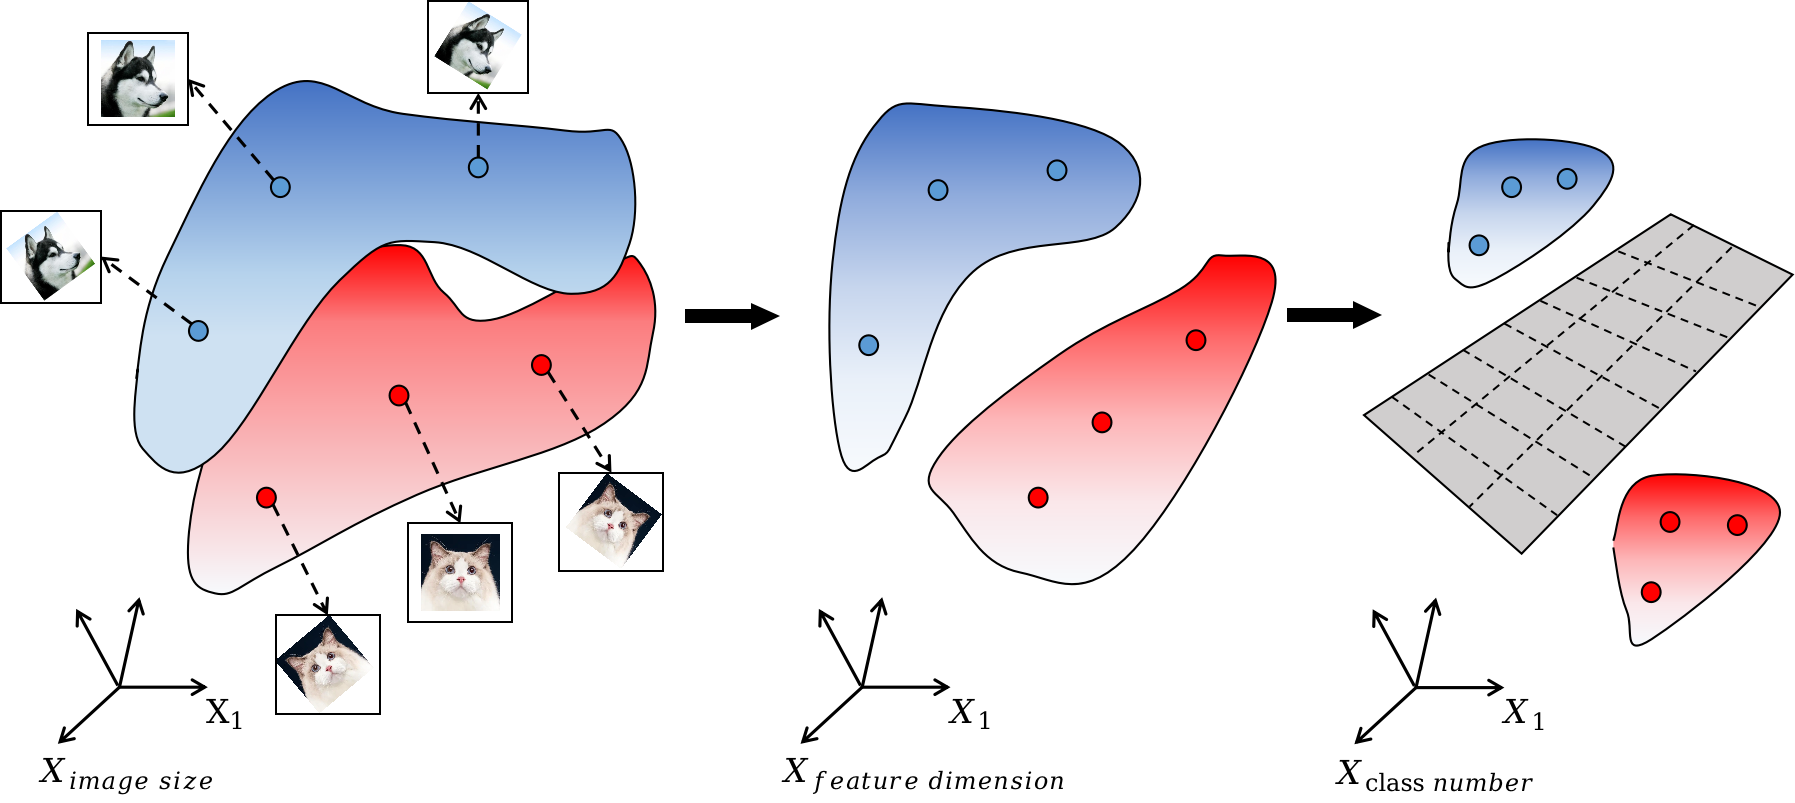
\includegraphics[width=1\columnwidth]{fig24}
\vskip -0.1in
\caption{Changes in the geometry of data manifolds as they are transformed in a deep neural network. The classification process of the data includes untangling the manifolds from each other and separating the different manifolds.}
\label{fig25}
\end{center}
\vskip -0.1in
\end{figure*}

\subsection{A Geometric Perspective on Data Classification\label{J.2}}

Natural datasets have intrinsic patterns that can be generalized to the manifold distribution principle: the distribution of a class of data is close to a low-dimensional manifold. As shown in Figure \ref{fig25}, data classification can be regarded as the unwinding and separation of manifolds. When a data manifold is entangled with other perceptual manifolds, the difficulty of classifying that manifold increases. Typically, a deep neural network consists of a feature extractor and a classifier. Feature learning can be considered as manifold unwinding, and a well-learned feature extractor is often able to unwind multiple manifolds for the classifier to decode. In this view, all factors about the manifold complexity may affect the model's classification performance. Therefore, we suggest that future work can explore the inter-class long-tailed problem from a geometric perspective.


\subsection{Introduce Semantic Scale Imbalance in Object Detection\label{J.3}}

Long-tailed distribution is one of the main difficulties faced by object detection algorithms in real-world scenarios. The classical object detection algorithms are generally trained on some manually designed datasets with relatively balanced data distribution. In contrast, the accuracy of these algorithms tends to suffer significantly on long-tailed distributed datasets. So far, methods for foreground-background imbalance and class imbalance have been proposed extensively, but these methods are based on the number of objects to define the degree of imbalance and cannot explain more phenomena. We will give examples below.

In the field of object detection, it is often encountered that although a class does not appear frequently, the model can always detect such instances efficiently. It is easy to observe that classes with simple patterns are usually easier to learn, even if the frequency of such classes is low. Therefore, classes with low frequency in object detection are not necessarily always harder to learn. We believe that it is a valuable research direction to analyze the richness of the instances contained in each class, and then pay more attention to the hard classes. The dimensionality of all images or feature embeddings in the image classification task is the same, which facilitates the application of the semantic scale proposed in this paper. However, the non-fixed dimensionality of each instance in the field of object detection brings new challenges, so we have to consider the effect of dimensionality on the semantic scale, which is a direction worthy of further study.

\subsection{Challenges of class imbalance in deep learning\label{J.4}}

Class imbalance remains a major challenge in the field of deep learning. Data imbalance classification, although widely studied, still lacks effective and clear methods and guidelines. The problem of object detection for class imbalance is still in its infancy and requires a greater investment of attention. In the following, we summarize the important future challenges and research directions in this field.

\begin{itemize}
     \item[(1)] \emph{The more precise measure of class difficulty}. An increasing number of studies have shown that the sample number does not accurately reflect the accuracy of the model in recognizing classes. Therefore, more extensive measures should be proposed to redefine the long-tail distribution to facilitate classification and object detection tasks and further expand the scope of research on long-tailed recognition. For example, a dataset with perfectly balanced sample numbers may not be balanced under other measures.

\begin{figure*}[h]% 纵向8行,图片靠右,宽度12.5em
\begin{center}
\vskip -0.14in
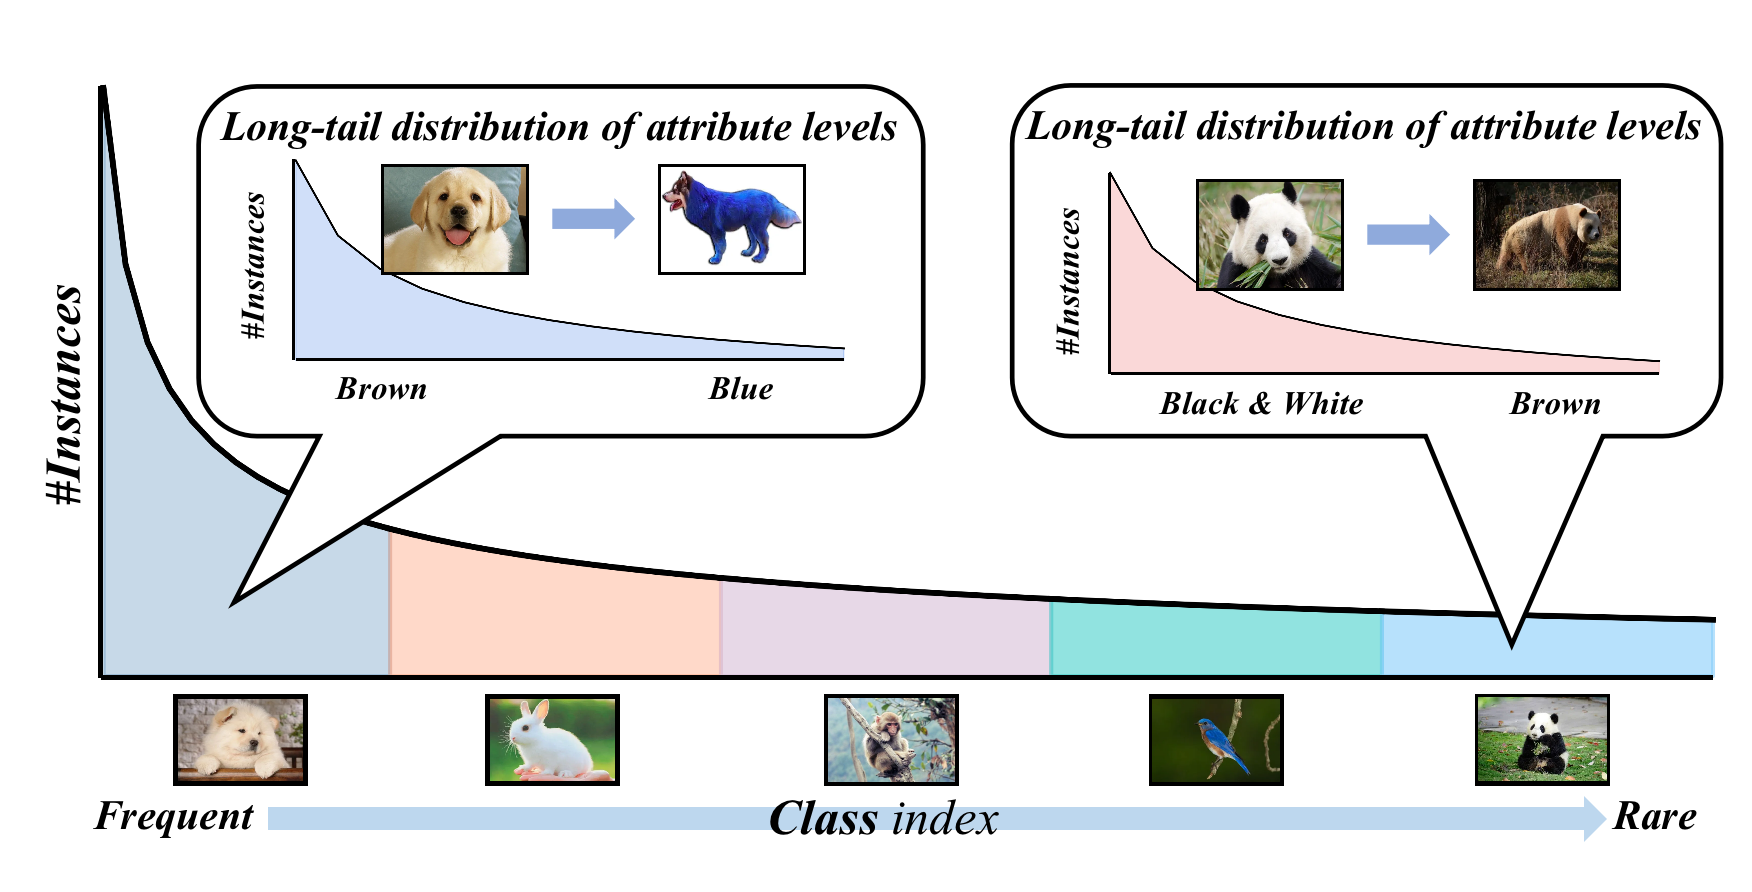
\includegraphics[width=0.95\columnwidth]{nfig35}
\vskip -0.2in
\caption{Class-level long-tailed distribution and intra-class attribute long-tailed distribution.}
\label{fig26}
\end{center}
\vskip -0.15in
\end{figure*}

     \item[(2)] \emph{Long-tailed distribution of properties in classes}. As shown in Figure \ref{fig26} \cite{paper115}, previous studies have focused on the imbalance between classes and ignored the imbalance of properties within each class. For example, most pandas have black and white fur, and only a small proportion of pandas are brown. In visual recognition tasks, we should not only pursue the overall accuracy of the class but also pay attention to whether samples with sparse properties in a class can be classified accurately. In medical image classification, the above point is particularly important. For example, pulmonary diseases contain many different types of diseases, and generally the more severe the disease tends to have a smaller sample number, suggesting that there is an imbalance of properties under the label of pulmonary disease. We hope to be able to recognize more severe diseases more accurately so that patients do not miss the best time to treat them.

     \item[(3)] \emph{Generalization performance of the model outside the training domain of the tail class}. As shown in Figure \ref{fig27}, tail classes often have very few samples, so these samples do not well represent the true distribution of the tail classes, which results in the model consistently failing to learn and adapt to the tail classes correctly. Obviously, recovering the underlying distribution of the tail classes helps the generalization performance of the model outside the training domain of the tail classes. It is currently shown that similar classes have similar distribution statistics (variance), which can lead researchers to recover the underlying distribution of tail classes. However, the current research is still in its infancy, and it is not a sufficiently stringent assumption that similar classes have similar variances. Therefore, we hope that in the future researchers will be able to help recover the true distribution of tail classes by more means.

\begin{figure*}[h]% 纵向8行,图片靠右,宽度12.5em
\begin{center}
%\vskip -0.08in
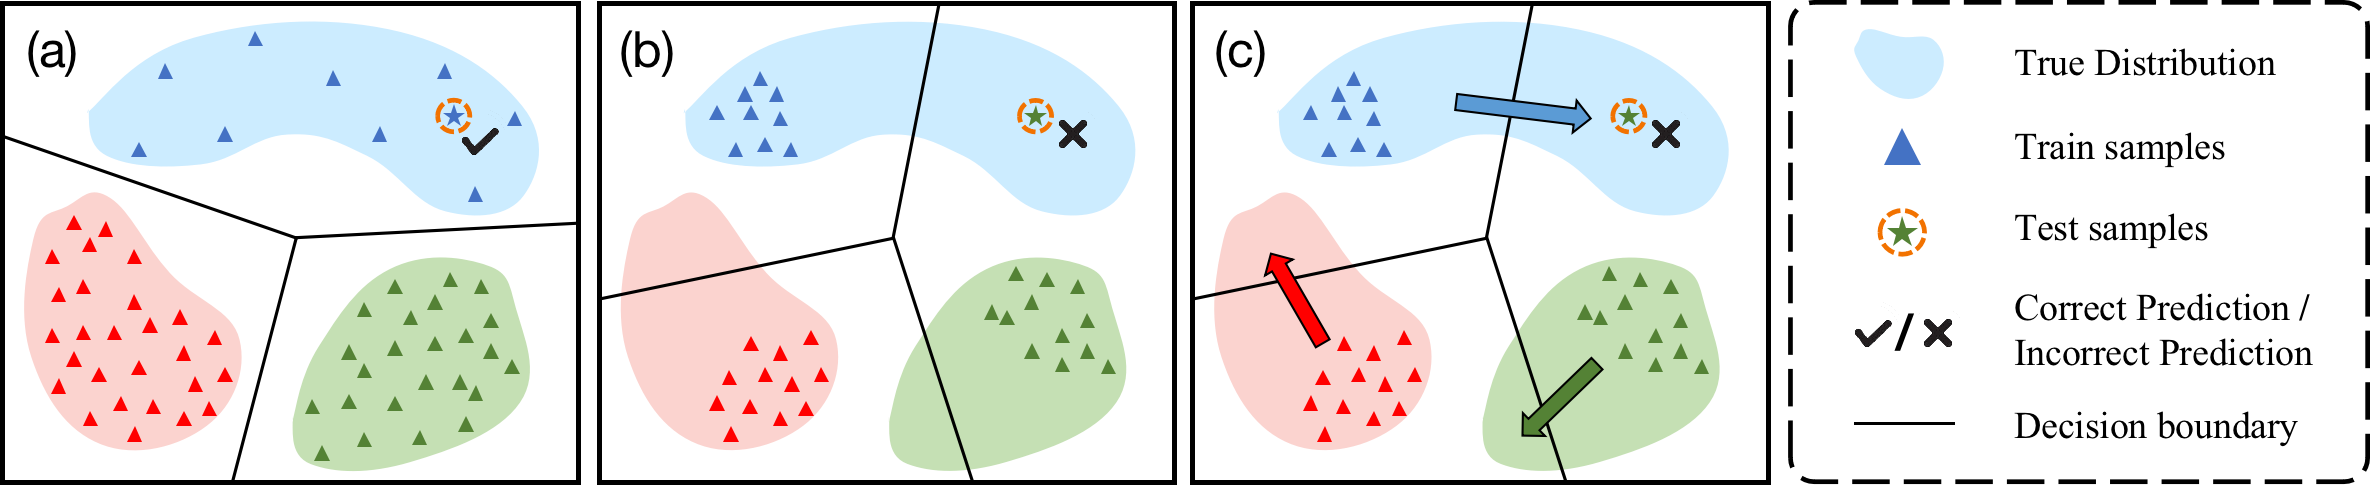
\includegraphics[width=1\columnwidth]{fig1a}
\vskip -0.05in
\caption{(a) When the samples uniformly cover the true data distribution, the model can learn the correct decision boundaries and can correctly classify unfamiliar samples to be tested. (b) When the samples cover only a portion of the true distribution, unfamiliar samples to be tested are highly likely to be misclassified due to the error in the decision boundary. (c) The direction in which the arrow points is the best direction to expand the sample.}
\label{fig27}
\end{center}
\vskip -0.13in
\end{figure*}

     \item[(4)] \emph{How to choose the appropriate long-tailed recognition method in the task}. Up to now, a large number of visual recognition methods on long-tail distribution have been proposed. While individual methods have positive performance in long-tailed recognition tasks, some combinations of methods may have negative effects. Few studies have focused on the selection and combination of different training techniques and methods. In the future, it is possible to explore how to select existing methods on specific tasks, and further, effective combinations of different methods are important. 
     \item[(5)] \emph{Multi-domain deep long-tailed learning}. Past research has typically focused on the problem of long-tailed distribution over a single domain, which has limited the research ideas. As shown in Figure \ref{fig28}, data from multiple domains can complement each other to alleviate the long-tailed distribution of classes \cite{paper119}. For example, in plant and animal classification, cameras are placed in different places to capture animals, but some animals only appear in a fixed area, which leads to different label distributions for animals captured by different cameras. But by combining the data from all cameras, a more balanced class can be obtained. Similarly, a similar situation occurs in other practical applications. For example, in a visual recognition problem, the few classes from "photo" images can be complemented by a potentially rich sample from "sketch" images. In autonomous driving, a few classes of "real" life accidents can be enriched by accidents generated in "simulations". In addition, in medical diagnosis, data from different populations can be mutually augmented, e.g., a small sample from one institution can be combined with the majority of possible instances from other institutions. In these examples, different data types can act as different domains, and such multi-domain data can also be utilized effectively to address data imbalances.

\begin{figure*}[h]% 纵向8行,图片靠右,宽度12.5em
\begin{center}
%\vskip -0.14in
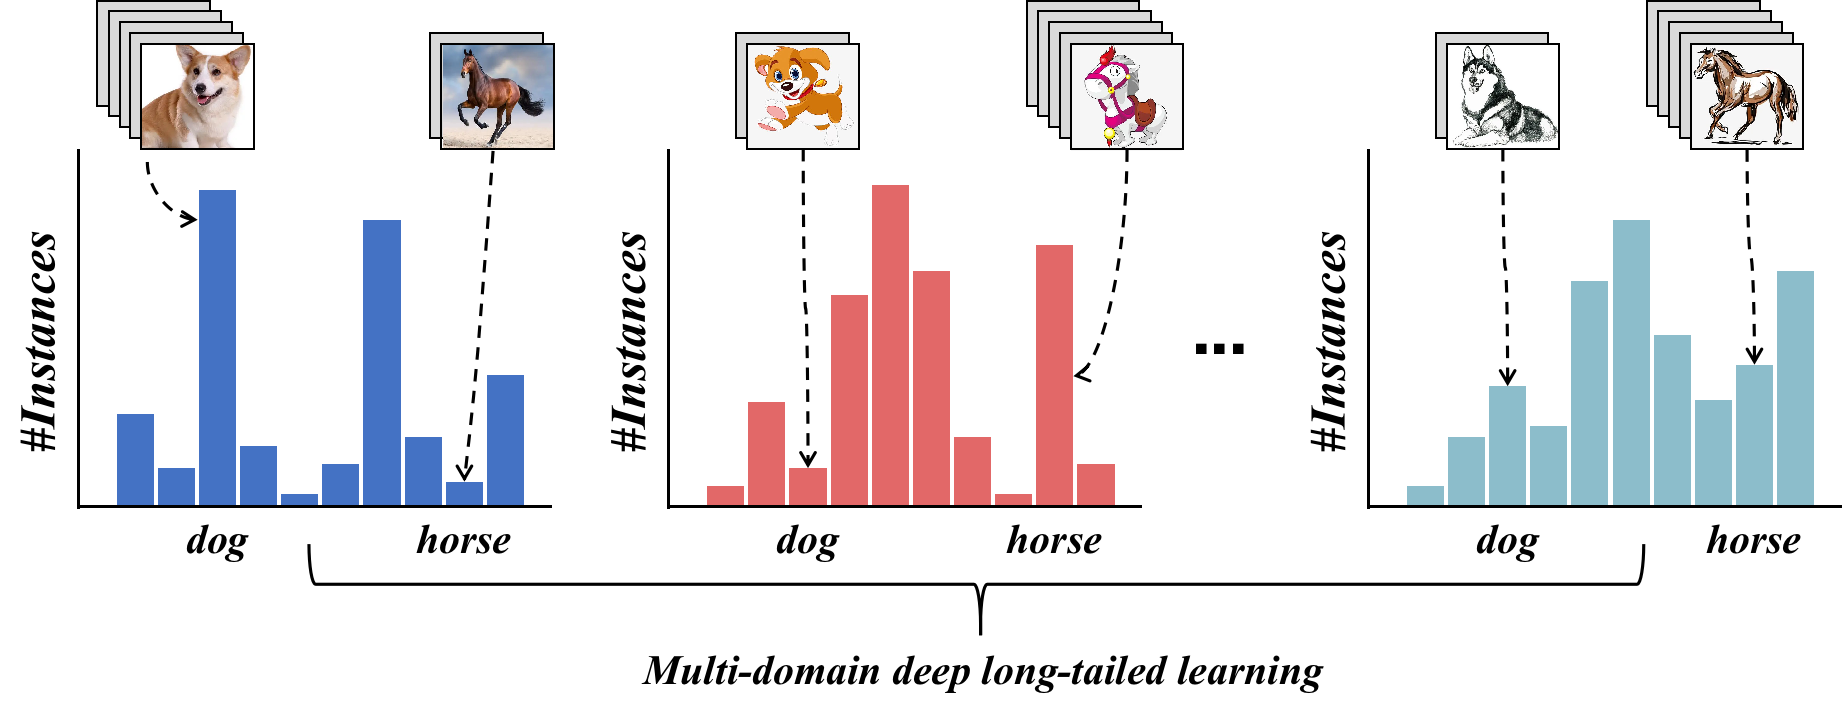
\includegraphics[width=1\columnwidth]{fig36}
\vskip -0.15in
\caption{The frequency of the same class appearing in different domains may differ significantly, assuming a smaller sample of horses in the real world and a larger number of horses in cartoon form. Images from different domains can complement each other to form a dataset with a balanced sample number. The purpose of multi-domain deep long-tailed learning is to train unbiased models using data from multiple domains and generalize over all domains.}
\label{fig28}
\end{center}
\vskip -0.12in
\end{figure*}

     \item[(6)] \emph{Recognition of unbalanced data streams}. Continuous learning aims to process new data that is continuously generated in order to dynamically update and adapt the model to the latest data domain. Challengingly, as new data is generated, the degree of imbalance between classes changes and what used to be a tail class may become a head class. The long-tailed distribution of properties within classes can also affect the performance of the model if concept drift occurs. Thus the key to handling unbalanced data streams is to evaluate the class-level difficulty and the long-tailed distribution of properties within classes in real time, which is a huge challenge. 
     \item[(7)] \emph{Augmentation methods for other modally unbalanced data}. Methods for multi-sample synthesis are widely used in image data augmentation, such as Mixup and Cutout, but there is still a lack of data augmentation methods for other modal data (e.g., speech and table). Researchers can design a more general method to generate samples of any type of data.
     \item[(8)] \emph{Other long-tailed visual recognition tasks}. Current research focuses on long-tail image classification, while less attention has been paid to long-tail object detection, image segmentation, and regression tasks. In object detection, there are multiple imbalances, such as foreground-background imbalance and imbalance between classes belonging to the foreground, which are unresolved challenges. With further applications of deep learning, research on imbalance learning in various fields will be of great benefit for real-world applications.
\end{itemize}

This study suggests some future avenues of inquiry to further deepen and expand the study of unbalanced learning. Of course, the scope of future inquiry into unbalanced learning is not limited to the eight challenges mentioned above, and we believe that new questions will arise in the course of inquiry into these eight challenges, but that researchers will eventually address them over time.

\epigraph{\emph{In everything balance has to be gained. Through balance you will come nearer to truth, because truth is the ultimate balance}.}{Osho}

\iffalse
\newpage

\hypersetup{hidelinks} 
\tableofcontents
\listoffigures
\listoftables

\fi





\iffalse
\begin{abstract}
As a popular paradigm for juggling data privacy and collaborative training, federated learning~(FL) is flourishing to distributively process the large scale of heterogeneous datasets on edged clients. Due to bandwidth limitations and security considerations, it ingeniously splits the original problem into multiple subproblems to be solved in parallel, which empowers \textit{primal dual} solutions to great application values in FL. In this paper, we review the recent development of classical \textit{federated primal dual} methods and point out a serious common defect of such methods in non-convex scenarios, which we say is a ``dual drift'' caused by dual hysteresis of those longstanding inactive clients under partial participation training. To further address this problem, we propose a novel \textit{\textbf{A}ligned \textbf{Fed}erated \textbf{P}rimal \textbf{D}ual}~(\textit{\textbf{A-FedPD}}) method, which constructs virtual dual updates to align global consensus and local dual variables for those protracted unparticipated local clients. Meanwhile, we provide a comprehensive analysis of the optimization and generalization efficiency for the \textit{A-FedPD} method on smooth non-convex objectives, which confirms its high efficiency and practicality. Extensive experiments are conducted on several classical FL setups to validate the effectiveness of our proposed method. 
\end{abstract}

%%%%%%%%%%%%%%%%%%%%%%%%%%%%%%%%%%%%%%%%%%%%%%%%%%
\section{Introduction}
\label{main:sec:introduction}
%%%%%%%%%%%%%%%%%%%%%%%%%%%%%%%%%%%%%%%%%%%%%%%%%%

\glsresetall

% \ljh{Just a draft. need polishing and proofreading}
A \gls{np}~\citep{garnelo2018conditional,garnelo2018neural} meta-learns a stochastic process describing the relationship between inputs and outputs in a given data stream, where each task in the data stream consists of a meta-training set of input-output pairs and also a meta-validation set. The \gls{np} then defines an implicit stochastic process whose functional form is determined by a neural network taking the meta-training set as an input, and the parameters of the neural network are optimized to maximize the predictive likelihood for the meta-validation set. This approach is philosophically different from the traditional learning pipeline where one would first elicit a stochastic process from the known class of models (e.g., \glspl{gp}) and hope that it describes the data well. An ideal \gls{np} would assume minimal inductive biases and learn as much as possible from the data. In this regard, \glspl{np} can be framed as a ``data-driven'' way of choosing proper stochastic processes.

 An important design choice for a \gls{np} model is how to capture the uncertainty in the random functions drawn from stochastic processes. When mapping the meta-training set into a function, one might employ a deterministic mapping as in \citet{garnelo2018conditional}. However, it is more natural to assume that there may be multiple plausible functions that might have generated the given data, and thus encode the functional (epistemic) uncertainty as a part of the \gls{np} model. \citet{garnelo2018neural} later proposed to map the meta-training set into a fixed dimensional \emph{global latent variable} with a Gaussian posterior approximation. While this improves upon the vanilla model without such a latent variable~\citep{le2018empirical}, expressing the functional uncertainty only through the Gaussian approximated latent variable has been reported to be a bottleneck~\citep{louizos2019functional}. To this end, \citet{lee2020bootstrapping} and \citet{lee2022neural} propose to apply bootstrap to the meta-training set to use the uncertainty arising from the population distribution as a source for the functional uncertainty.

In this paper, we take a rather different approach to define the functional uncertainty for \glspl{np}. Specifically, we utilize the martingale posterior distribution~\citep{fong2021martingale}, a recently developed alternative to conventional Bayesian inference. In the martingale posterior, instead of eliciting a likelihood-prior pair and inferring the Bayesian posterior, we elicit a joint predictive distribution on future data given observed data. Under suitable conditions on such a predictive distribution, it can be shown that the uncertainty due to the generated future data indeed corresponds to the uncertainty of the Bayesian posterior. Following this, we endow a \gls{np} with a joint predictive distribution defined through neural networks and derive the functional uncertainty as the uncertainty arising when mapping the randomly generated future data to the functions. Compared to the previous approaches of either explicitly positing a finite-dimensional variable encoding the functional uncertainty or deriving it from a population distribution, our method makes minimal assumptions about the predictive distribution and gives more freedom to the model to choose the proper form of uncertainty solely from the data. Due to the theory of martingale posteriors, our model guarantees the existence of the martingale posterior corresponding to the valid Bayesian posterior of an implicitly defined parameter. 
% \ed{Does the following make sense: }
Furthermore, working in the space of future observations allows us to incorporate the latent functional uncertainty path with deterministic path in a more natural manner.
% \ljh{It would be good to have more concrete motivation to prefer the martingale posteriors over conventional Bayesian inference; what would be an advantage of doing that, aside from the fact that we don't need to choose likelihood and prior?} \ed{I'll have a think about this, and will also do some proofreading. Because of the time difference and my job hours, timing might be a bit tricky tomorrow. When would be the best time for me to proofread?}

We name our extension of \glspl{np} with the joint predictive generative models as the \gls{mpnp}. Throughout the paper, we propose an efficient neural network architecture for the generative model that is easy to implement, flexible, and yet guarantees the existence of the martingale posterior. We also propose a training scheme to stably learn the parameters of \glspl{mpnp}. Using various synthetic and real-world regression tasks, we demonstrate that \gls{mpnp} significantly outperforms the previous \gls{np} variants in terms of predictive performance.





% \gls{npf}~\citep{garnelo2018conditional, garnelo2018neural} is a class of parametric models which defines stochastic processes over given data using neural networks.
% Unlike classical stochastic processes (e.g. \glspl{gp}), \gls{npf} learns to fit a proper stochastic processes from data under meta-learning framework.
% The deterministic version of \gls{npf}, \glspl{cnp}~\citep{garnelo2018conditional} deterministically map each dataset to a certain stochastic process which does not consider functional uncertainty.
% In order to compensate for this problem, \glspl{np}~\citep{garnelo2018neural} introduce a global latent variable which captures functional uncertainty.
% \citet{le2018empirical} empirically shows that considering functional uncertainty in \glspl{np} improves the diversity in function realizations and the predictive performance for data.

% Although \glspl{np} tries to capture functional uncertainty, there is some limitations for \glspl{np} to well capture uncertainty with a Gaussian latent variable.
% To overcome this problem, there are some prior works which applying advanced functional uncertainty modeling strategies~\citep{lee2020bootstrapping}\citep{lee2022neural} instead of a global latent variable.
% \gls{bnp}~\citep{lee2020bootstrapping} employs the residual bootstrapping strategy to make more robust uncertainty estimation even for the data-model mismatch situation. 
% However, \gls{bnp} requires a high computational cost compared to \gls{np} due to it's residual bootstrapping strategy.
% \gls{neubnp}~\citep{lee2022neural} employs the recent computationally efficient bootstrapping of the neural network called Neural Bootstrapper~\citep{shin2021neural}.
% However, \gls{neubnp} multiplies Dirichlet distributed random bootstrap weights to features of context dataset which disturbs model to well recovers the given dataset.

% This paper presents a novel extension of \gls{npf} which introduces functional uncertainty by changing posterior uncertainty on function parameters as predictive uncertainty on the unseen data conditional on the observed data...


\section{Related Work}
\label{sec:recent-work}

Traditional methods \cite{Carhart:1985ap,Nilakantan:1987tt,Rogers:2010fp} represent molecular structures with fingerprints. Some prior studies \cite{Svetnik:2004ab,Meyer:2019ld,Wu:2018dv} employ tree-based machine leaning models such as random forests \cite{Breiman:2001rf} and XGBoost \cite{Chen:2016ga} on fingerprints to predict the properties of molecules.
With the development of deep learning, neural approaches have been dominating the field given their strong representation ability.
One line of work \cite{Wang:2019hp,Chithrananda:2020eo} leverages language modeling techniques such as BERT \cite{Devlin:2019uk} to learn molecular representations based on SMILES strings \cite{Weininger:1988sm}.
However, some argue that sequence-based representations cannot fully capture substructure information and propose to leverage Graph Neural Networks (GNNs), which model molecules as graphs with atoms as nodes and bonds as edges \cite{Gilmer:2017tl,Liu:2019uy,Ying:2021ug}.
Despite the prosperous progress, they only model 2D topological structures of molecules, without considering the 3D coordinates of atoms that are known to determine certain chemical and physical functionalities of molecules.
To address this deficiency, recent work further explicitly considers such 3D geometry and designs equivariant networks to obtain the representations \cite{Schutt:2017wh,Klicpera:2020vw,Satorras:2021tz,Fuchs:2020wj,Schutt:2021vm,Du:2021ci,Liu:2021hq,Gasteiger:2021uf,Batzner:2021to,Brandstetter:2022wl,Xu:2021uj}.

Even though molecular representation learning techniques have been extensively investigated, there are very few labeled datasets available for studying the molecular properties of interest (e.g., drug-likeness or quantum properties).
On the other hand, there are abundant unannotated molecules available, which motivates researchers to study pretraining techniques that learn the model weights in a self-supervised manner and transfer the knowledge to downstream datasets with limited annotations via fine-tuning.
A series of pretraining frameworks on 2D molecular graph representations have been developed so far \cite{Rong:2020vk,Hu:2020uz,Zhang:2021wj,Wang:2022gr,Li:2020fo,Xia:2022jw}.
Recent work GEM \cite{Fang:2022et} studies large-scale pretraining for 3D geometry representations.
Additionally, researchers also study to supplement 2D-graph-based pretraining with 3D conformation information \cite{Yang:2021wg,Liu:2022vr,Stark:2021ug}.

A succinct comparison of our work with other representative methods is provided in \cref{tab:comparison-baseline}.
Compared to the above studies, our proposed \themodel is the only model that can \emph{adaptively} leverage multiple featurizations for both pretraining and fine-tuning stages.

\begin{table}
	\centering
	\rowcolors{2}{white}{lightgray!10}
	\caption{Comparing \themodel with representative self-supervised methods on molecular pretraining.}
	\begin{tabular}{l*{8}{c}}
	\toprule
	& \multicolumn{4}{c}{Pretraining} & \multicolumn{4}{c}{Fine-tuning} \\
	\cmidrule(lr){2-5} \cmidrule(lr){6-9}
	\rowcolor{white} \multirow{-2.5}{*}{Method} & 2D & 3D & Fingerprint & SMILES & 2D & 3D & Fingerprint & SMILES \\
	\midrule
	SMILES-BERT \cite{Wang:2019hp} & & & & \cmark & & & & \cmark \\
	ChemBERTa \cite{Chithrananda:2020eo} & & & & \cmark & & & & \cmark \\
%	GraphSAGE \cite{Hamilton:2017tp} & \cmark & & & & \cmark & & & \\
	AttrMask, ContexPred \cite{Hu:2020uz} & \cmark & & & & \cmark & & & \\
%	GPT-GNN \cite{Hu:2020vh} & \cmark & & & & \cmark & & & \\
%	InfoGraph \cite{Sun:2020vi} & \cmark & & & & \cmark & & & \\
	GraphCL \cite{You:2020ut} & \cmark & & & & \cmark & & & \\
%	JOAO \cite{You:2021wl} & \cmark & & & & \cmark & & &  \\
	GraphLoG \cite{Xu:2021tv} & \cmark & & & & \cmark & & & \\
	GROVER \cite{Rong:2020vk} & \cmark & & & & \cmark & & & \\
	GEM \cite{Fang:2022et} & & \cmark & & & & \cmark & & \\
	3D Infomax \cite{Stark:2021ug} & \cmark & \cmark & & & \cmark & & &  \\
	GraphMVP \cite{Liu:2022vr} & \cmark & \cmark & & & \cmark & & &  \\
	\themodel (Ours) & \cmark & \cmark & \cmark & \cmark & \cmark & \cmark & \cmark & \cmark \\
	\bottomrule
	\end{tabular}
	\label{tab:comparison-baseline}
\end{table}



%%%%%%%%%%%%%%%%%%%%%%%%%%%%%%%%%%%%%%%%%%%%%%%%%%
\section{Background}
\label{main:sec:background}
%%%%%%%%%%%%%%%%%%%%%%%%%%%%%%%%%%%%%%%%%%%%%%%%%%
\subsection{Settings and notations}

Let $\calX = \bbR^{\din}$ be an input space and $\calY = \bbR^\dout$ be an output space. 
We are given a set of \emph{tasks} drawn from an (unknown) task distribution, $\tau_1, \tau_2, \dots \iidsim p_\text{task}(\tau)$. 
A task $\tau$ consists of a dataset $Z$ and an index set $c$, where $Z = \{z_i\}_{i=1}^n$ with each $z_i = (x_i, y_i) \in \calX \times \calY$ is a pair of an input and an output. We assume $Z$ are i.i.d. conditioned on some function $f$. The index set $c \subsetneq [n]$ where $[n] := \{1,\dots, n\}$ defines the \emph{context set} $Z_c = \{z_i\}_{i\in c}$. The \emph{target set} $Z_t$ is defined similarly with the index $t := [n]\setminus c$.

% Let $\calX = \bbR^{\din}$ be an input space and $\calY = \bbR^\dout$ be an output space. 
% We are given a set of \emph{tasks} drawn from an (unknown) task distribution, $\tau_1, \tau_2, \dots \iidsim p_\text{task}(\tau)$. 
% Each task $\tau$ consists of a tuple $\calD = (X, Y)$ and an index set $c \subsetneq [n]$ where $[n] := \{1,\dots, n\}$. Here, $X = \{x_i\}_{i=1}^n$ is an input set with $x_i \in \calX$ and $Y = \{y_i\}_{i=1}^n$ is an output set with $y_i \in \calY$. The \emph{context set} indexed by $c$ is then defined as $\calD_c = (X_c, Y_c)$ with $X_c = \{x_i\}_{i\in c}$ and $Y_c = \{y_i\}_{i\in c}$. The \emph{target} index set $t$ is defined as $t := [n] \setminus c$, and the corresponding target set $\calD_t$ is defined similarly.

%%%%%%%%%%%%%%%%%%%%%%%%%%%%%%%%%%%%%%%%%%%%%%%%%%
\subsection{Neural process families}

Our goal is to train a class of random functions $f: \calX \to \calY$ that can effectively describe the relationship between inputs and outputs included in a set of tasks. Viewing this as a meta-learning problem, for each task $\tau$, we can treat the context $Z_c$ as a meta-train set and target $Z_t$ as a meta-validation set. We wish to meta-learn a mapping from the context $Z_c$ to a random function $f$ that recovers the given context $Z_c$ (minimizing meta-training error) and predicts $Z_t$ well (minimizing meta-validation error). Instead of directly estimating the infinite-dimensional $f$, we learn a mapping from $Z_c$ to a predictive distribution for finite-dimensional observations,
\[
p(Y | X, Z_c) = \int \bigg[\prod_{i\in c} p(y_i | f, x_i) \prod_{i\in t} p(y_i | f, x_i)\bigg] p(f|Z_c) \dee f,
\]
where we are assuming the outputs $Y$ are independent given $f$ and $X$. We further restrict ourselves to simple heteroscedastic Gaussian measurement noises,
\[
p(y|f, x) = \calN(y | \mu_\theta(x), \sigma^2_\theta(x)I_{\dout}),
\]
where $\mu_\theta: \calX \to \calY$ and $\sigma_\theta^2: \calX \to \bbR_+$ map an input to a mean function value and corresponding variance, respectively. $\theta \in \bbR^{h}$ is a parameter indexing the function $f$, and thus the above predictive distribution can be written as
\[
p(Y | X, Z_c) = \int 
\bigg[\prod_{i\in [n]} \calN(y_i|\mu_\theta(x_i), \sigma_\theta^2(x_i) I_\dout)\bigg] p(\theta|Z_c) \dee \theta.
\]
A \gls{np} is a parametric model which constructs a mapping from $Z_c$ to $\theta$ as a neural network. The simplest version, \gls{cnp}~\citep{garnelo2018conditional}, assumes a deterministic mapping from $Z_c$ to $\theta$ as
\[
p(\theta|Z_c) = \delta_{r_c}(\theta), \quad r_c = f_\text{enc}(Z_c ; \phi_\text{enc}),
\]
where $\delta_{a}(x)$ is the Dirac delta function (which gives zero if $x\neq a$ and $\int\delta_a(x) \dee x=1$) and $f_\text{enc}$ is a \emph{permutation-invariant} neural network taking sets as inputs~\citep{zaheer2017deep}, parameterized by $\phi_\text{enc}$. Given a summary $\theta= r_c$ of a context $Z_c$, the \gls{cnp} models the mean and variance functions $(\mu, \sigma^2)$ as
\[
(\mu_\theta(x), \log \sigma_\theta(x)) = f_\text{dec}(x, r_c ; \phi_\text{dec}),
\]
where $f_\text{dec}$ is a feed-forward neural network parameterized by $\phi_\text{dec}$. Here the parameters $(\phi_\text{enc}, \phi_\text{dec})$ are optimized to maximize the expected predictive likelihood over tasks, $\bbE_{\tau}[\log p(Y|X, Z_c)]$.

Note that in the \gls{cnp}, the mapping from $Z_c$ to $\theta$ is deterministic, so it does not consider \emph{functional uncertainty} or epistemic (model) uncertainty. To resolve this, \citet{garnelo2018neural} proposed \gls{np} which learns a mapping from an arbitrary subset $Z' \subseteq Z$ to a variational posterior $q(\theta|Z')$ approximating $p(\theta|Z')$ under an implicitly defined prior $p(\theta)$: 
\[
(m_{Z'}, \log s_{Z'}) = f_\text{enc}(Z'; \phi_\text{enc}), \quad p(\theta|Z') \approx q(\theta|Z') := \calN(\theta | m_{Z'}, s^2_{Z'}I_h).
\]
With $f_\text{enc}$, the \gls{elbo} for the predictive likelihood is written as
\[
\log p(Y|X,Z_c) &\geq \sum_{i\in[n]} \bbE_{q(\theta|Z)}[\log \calN(y_i|\mu_\theta(x_i), \sigma_\theta^2(x_i)I_\dout)] - \KL[q(\theta|Z)\Vert p(\theta|Z_c)] \nonumber\\
&\approx
\sum_{i\in[n]} \bbE_{q(\theta|Z)}[\log \calN(y_i|\mu_\theta(x_i), \sigma_\theta^2(x_i)I_\dout)] - \KL[q(\theta|Z)\Vert q(\theta|Z_c)].
\]
An apparent limitation of the \gls{np} is that it assumes a uni-modal Gaussian distribution as an approximate posterior for $q(\theta|Z_c)$. Aside from the limited flexibility, it does not fit the motivation of \glspl{np} trying to learn as much as possible in a data-driven manner, as pre-specified parametric families are used.  

There have been several improvements over the vanilla \glspl{cnp} and \glspl{np}, either by introducing attention mechanism~\citep{vaswani2017attention} for $f_\text{enc}$ and $f_\text{dec}$~\citep{kim2018attentive}, or using advanced functional uncertainty modeling~(\citealp{lee2020bootstrapping}; \citealp{lee2022neural}). We provide a detailed review of the architectures for such variants in \cref{app:sec:architectures}. Throughout the paper, we will refer to this class of models as \gls{npf}.

% \subsection{Neural Process Family}
% Consider a target dataset $\calD=(X,Y)$ where $X=\{x_i\}_{i=1}^n$ is an input set and $Y=\{y_i\}_{i=1}^n$ is an output set. 
% Here we define subset $\calD_C=(X_C,Y_C)=\{(x_i,y_i)\}_{i\in C}$ as our context dataset where $C\subsetneq [n]$ denotes an index set.
% With these $\calD$ and $\calD_C$, \gls{npf}\citep{garnelo2018conditional, garnelo2018neural} learns to make a stochastic process which maps $x\in X$ to some conditional distribution $p(y|x,X_C,Y_C)$ by maximizing
% \begin{align}
%     \log p(Y|X,\calD_C) = \sum_{i=1}^n \log p(y_i|x_i, \calD_C)=\sum_{i=1}^n \log p(y_i|x_i,X_C,Y_C).
% \end{align}
% The deterministic \gls{npf} called \glspl{cnp}~\citep{garnelo2018conditional, gordon2020convolutional} predicts $p(y_i|x_i, X_C,Y_C)$ only with deterministic path which is made up with an \textit{permutation invariant}~\citep{zaheer2017deep} encoder neural network $f_{\enc}$ and a decoder neural network $f_{\dec}$.
% Here an encoder neural network $f_{\enc}$ compresses $(X_C,Y_C)$ into a feature $r_C$.
% A decoder neural network $f_{\dec}$ takes $r_C$ and $x_i$ as inputs and outputs the parameters of the distribution $p(y_i|x_i,X_C,Y_C)$.
% The conditional distribution $p(y_i|x_i,X_C,Y_C)$ is usually modelled as a Gaussian distribution.
% We can simplify these procedures as:
% \begin{align}
%     r_C = f_\enc(X_C,Y_C), \quad (\mu_i, \log\sigma_i)=f_\dec(x_i,r_C),\quad  p(y_i|x_i,X_C,Y_C)=\calN(y_i|\mu_i,\sigma_i^2).
% \end{align}

% The stochastic \gls{npf} called \glspl{np}~\citep{garnelo2018neural,foong2020meta} contains a latent path in addition to deterministic path to predict $p(y_i|x_i, X_C,Y_C)$.
% This latent path has an own permutation invariant latent encoder neural network $f_{\lat}$ and shares a decoder neural network $f_{\dec}$.
% $f_\lat$ takes $(X_C,Y_C)$ as an input and outputs the parameters of Gaussian distribution $p(z|X_C,Y_C)$ where $z$ is a global latent variable of \gls{np}.
% Global latent variable $z$ models a \textit{functional uncertainty} of \gls{np} which means that it helps \gls{np} to make the diverse conditional distribution $p(y_i|x_i,X_C,Y_C)$. With this latent path, the procedure of \glspl{np} can be summarized as:
% \begin{align}
%     &r_C = f_\enc(X_C,Y_C), \quad (\mu_z,\log\sigma_z)=f_\lat(X_C,Y_C),\quad z|\calD_C\sim\calN(\mu_z, \sigma_z^2)\\
%     &(\mu_i, \log\sigma_i)=f_\dec(x_i,r_C,z),\quad  p(y_i|x_i,X_C,Y_C)=\calN(y_i|\mu_i,\sigma_i^2).
% \end{align}
% In order to train \gls{np}, we can use ELBO of the conditional probability which is 
% \begin{align}
%     \log p(Y|X,\calD_C) \geq \sum_{i=1}^n \bbE_{q(z|\calD)}\left[\log p(y_i|x_i,z,r_C)\right]-\text{KL}(q(z|\calD)||p(z|\calD_C)).
% \end{align}
% If we approximate $p(z|\calD_C)$ by $q(z|\calD_C)$, this ELBO changes into our train loss function
% \begin{align}
%     \sum_{i=1}^n \bbE_{q(z|\calD)}\left[\log p(y_i|x_i,z,r_C)\right]-\text{KL}(q(z|\calD)||p(z|\calD_C)).
% \end{align}

%%%%%%%%%%%%%%%%%%%%%%%%%%%%%%%%%%%%%%%%%%%%%%%%%%
\subsection{Martingale Posterior Distributions}

The martingale posterior distribution \citep{fong2021martingale} is a recent generalization of Bayesian inference which reframes posterior uncertainty on parameters as {predictive} uncertainty on the unseen population conditional on the observed data. Given observed samples $Z = \{z_i\}_{i=1}^n$  i.i.d. from the sampling density $p_0$, one can define the parameter of interest as a functional of $p_0$, that is
$$
\theta_0 = \theta(p_0) =  \argmin_\theta\int \ell(z,\theta)\, p_0(dz), 
$$
where $\ell$ is a loss function. For example, $\ell(z,\theta) =  (z-\theta)^2$ would return $\theta_0$ as the mean, and $\ell(z,\theta)= - \log p(z \mid \theta)$ would return the KL minimizing parameter between $p(\cdot \mid \theta)$ and $p_0$.

The next step of the martingale posterior is to construct a \emph{joint} predictive density on $Z' = \{z_i\}_{i=n+1}^N$ for some large $N$, which we write as $p(Z' \mid Z)$. In a similar fashion to a bootstrap, one can imagine drawing $Z' \sim p(Z' \mid Z)$, then computing $\theta(g_N)$ where $g_N(z) = \frac{1}{N} \sum_{i=1}^N \delta_{z_i} (z)$. %\ljh{Define $\theta(g_N)$ somewhere?} 
The predictive uncertainty in $Z'$ induces uncertainty in $\theta(g_N)$ conditional on $Z$. The key connection is that  if $p(Z' \mid Z)$ is the Bayesian joint  posterior predictive density, and $\ell = - \log p(z \mid \theta)$, then $\theta(g_N)$ is distributed according to the Bayesian posterior $\pi(\theta \mid Z)$ as $N \to \infty$, under weak conditions. In other words, posterior uncertainty in $\theta$ is equivalent to predictive uncertainty in $\{z_i\}_{i=n+1}^\infty$. 

\cite{fong2021martingale} specify more general  $p(Z' \mid Z)$ directly beyond the Bayesian posterior predictive, and define the (finite) martingale posterior 
as 
$\pi_N(\theta \in A \mid Z) = \int \mathbbm{1}(\theta(g_N) \in A) \, p(dZ' \mid Z)$. In particular, the joint predictive density can be factorized into a sequence of 1-step-ahead predictives, 
$
p(Z' \mid Z) = \prod_{i=n+1}^N p(z_i \mid z_{1:i-1}),
$
and the sequence $\{p(z_i \mid z_{1:i-1})\}_{n+1}^N$ is elicited directly, removing the need for the likelihood and prior. Hyperparameters for the sequence of predictive distributions can be fitted in a data-driven way by maximizing 
$$\log p(Z) = \sum_{i=1}^n \log p(z_i \mid z_{1:i-1}),$$ 
which is analogous to the log marginal likelihood.  \cite{fong2021martingale} requires the sequence of predictives to be \gls{cid}, which is a martingale condition on the sequence of predictives that ensures $g_N$ exists almost surely. The Bayesian posterior predictive density is a special case, as exchangeability of $p(Z' \mid Z)$ implies the sequence of predictives is \gls{cid} In fact, De Finetti's theorem \citep{de1937prevision} guarantees that any exchangeable joint density implies an underlying likelihood-prior form, but specifying the predictive density directly can be advantageous. It allows for  easier computation, as we no longer require posterior approximations, and it also widens the class of available nonparametric predictives which we will see shortly.  

% \ljh{Will you describe what a ``martingale posterior'' actually is here? (Definition 1 in \citet{fong2021martingale})}.

% \ed{Just brainstorming some ideas below}

%  In the meta-learning context, for each $\tau_j \sim p(\tau)$, we are interested in  obtaining predictives $p_\phi( \mathcal{D}_c' \mid \mathcal{D}_c)$, where $\mathcal{D}_c' = \{z_i\}_{i = n+1:N}$ and $\mathcal{D}_c \mid \tau_j$ consists of i.i.d. samples. The log marginal likelihood for each task is $\log p(\mathcal{D}_c)$, so a valid training objective could be $E_\tau[\log p(\mathcal{D}_c)]$. However, as we specify $p(\mathcal{D}_c' \mid \mathcal{D}_c)$ directly, it is not obvious how to compute $\log p(\mathcal{D}_c)$. Instead, we could estimate this with  cross-validation, that is $p(\mathcal{D}_c^{\text{test}}\mid \mathcal{D}_c^{\text{train}})$, where $\mathcal{D}_c = \mathcal{D}_c^{\text{test}}\cup \mathcal{D}_c^{\text{train}}$. Or is there anything stopping us from using $p(\mathcal{D}_t \mid \mathcal{D}_c)$?
%  \ed{I was thinking $p(\calD_t|\calD_c)$ where $p$ is the generative model (not decoder), but I think this is very similar to $p(\mathcal{D}_c^{\text{test}}\mid \mathcal{D}_c^{\text{train}})$.}
%  \lhg{Ah... I see... Actually, I think we can't measure $p(\calD_t|\calD_c)$ without decoder. I also tried $p(\calD_c^{\text{test}}|\calD_c^{train})$ with decoder. }
%  \ed{Ah I see, because we only have a generative model right? That's a great motivator for the third term in (14) then. }
%  \lhg{yes. That's right:)}
%  {\textcolor{red}{Hyungi: I think we can try $p(\mathcal{D}_c^{\text{test}}\mid \mathcal{D}_c^{\text{train}})$ as our training objective and a minor curious point is "Is this training objective helps our generator to make some reasonable pseudo context data?". I think we have to check this with experiment. By the way $p(D_C''|D_C \cup (D_C'\textbackslash D_C''))$ loss did not work for directly generating pseudo context data framework.} }
 
%  \ed{{Maybe it makes sense that the old objective doesn't work too well, since $\mathcal{D}_C' $ is simulated from $p(\mathcal{D}_C' \mid \mathcal{D}_C)$, so it will always have high likelihood. Whereas checking the model on the actual observed $\mathcal{D}_c$ will force it to fit well?}}
 
%  \ed{Thanks for the update! By our feature model, do you mean the current objective in equation (14) performs the best? If so, maybe we should just stick to that then. We can also argue that it is somewhat difficult to estimate the density values $p(\mathcal{D}_C' \mid \mathcal{D}_C)$ as the predictive is generative, and the third term is kind of a proxy for this `marginal likelihood'. }
 
%  \lhg{Yeah, equation (14) performs the best. We are now doing some last trials on directly sampling version. As you said, I think we should stick to equation (14) and feature generating model.}
%  \ed{Nice, I think it's clear now and yes I agree :) I'll perhaps add a sentence after (14) to describe the lack of a tractable marginal likelihood density. Will comment out the above after.}
%  \lhg{That will be great for us. Thank you}
 
%  {\color{red} Edwin: Expand to meta-learning framework, may need discussion of amortization? Or leave in Section 3.1? }
%  {\color{red} Juho: I will discuss the amortization part in section 3.1.}

%%%%%%%%%%%%%%%%%%%%%%%%%%%%%%%%%%%%%%%%%%%%%%%%%%
\subsection{Exchangeable Generative Models}\label{main:subsec:exchangeable}

To construct a martingale posterior, we can either specify a sequence of one-step predictive distributions or the joint predictive density distribution directly, as long as the \gls{cid} condition is satisfied.  Here, we opt to specify an exchangeable $p(Z' \mid Z)$ directly, which then implies the required \gls{cid} predictives. We now briefly review exchangeable generative models which can be used to specify the exchangeable joint predictive.  For a set of random variables $Z = \{z_i\}_{i=1}^n$ with each $z_i\in \calZ = \bbR^{d}$, we say the joint distribution $p(Z)$ is \emph{exchangeable} if it is invariant to the arbitrary permutation of the indices, that is, $p(Z) = p(\pi\cdot Z)$ for any permutation $\pi$ of $[n]$. A simple way to construct such exchangeable random variables is to use a \emph{permutation-equivariant mapping}. A mapping $\bof: \calZ^n\to\calZ^n$ is permutation equivariant if $\bof(\pi\cdot Z) = \pi\cdot\bof(Z)$ for any $\pi$. Given $\bof$, we can first generate i.i.d. random variables and apply $\bof$ to construct a potentially correlated but exchangeable set of random variables $Z$ as follows:
\[
\calE := \{\varepsilon_i\}_{i=1}^n \iidsim p_0, \quad Z = \bof(\calE).
\]
For $\bof$, we employ the modules introduced in \citet{lee2019set}. Specifically, we use a permutation equivariant module called  \gls{isab}. An \gls{isab} mixes input sets through a learnable set of parameters called \emph{inducing points} via \glspl{mab}~\citep{vaswani2017attention,lee2019set}. 
\[
\textsc{isab}(\calE) = \textsc{mab}(\calE, H) \in \bbR^{n\times d}\text{ where } H = \textsc{mab}(I, \calE)\in \bbR^{m\times d}.
\]
Here, $I \in \bbR^{m\times d}$ is a set of $m$ inducing points and $\textsc{mab}(\cdot,\cdot)$ computes attention between two sets.
The time-complexity of an \gls{isab} is $O(nm)$, scales linear with input set sizes.

% \paragraph{Exchangeability}


% In order to generate a set structured data, model should satisfy a condition called \textit{exchangeability}~\citep{kim2021setvae}. Exchangeability condition means that the probability of generated set data does not depend on its ordering. To achieve exchangeability, a joint distribution of the generated set data should satisfy permutation invariance. In other words, for a set of random variables $\bX=\{X_i\}_{i=1}^n$ and for any permutation $\pi$, joint probability $p$ should satisfy:
% \begin{align}
%     p(\bX) = p(\pi(\bX)).
% \end{align}
% A nice and easy way to make a permutation invariant joint distribution is using a permutation equivariant function $f_{\text{per}}$ and \textit{i.i.d.} random variable set $\bX'=\{X_i'\}_{i=1}^n$ which is called \textit{permutation-equivariant generative framework}~\citep{kim2021setvae}.
% In this framework, if we let $\bX = f_{\text{per}}(\bX')$ then the joint distribution of $\bX$ satisfies permutation invariant.
% \paragraph{Set Transformer} Set Transformer~\citep{lee2019set} is an attention-based neural network model which satisfies permutation invariant property for input dataset. It contains permutation equivariant module called ISAB. ISAB transforms the input dataset $\bx\in\bbR^{n\times d}$ by a smaller set $I\in\bbR^{m\times d}$ called inducing points:
% \begin{align}
%     \text{ISAB}(\bx) &= \text{MAB}(\bx, \bH)\in\bbR^{n\times d},\\
%     \text{where } \bH &=\text{MAB}(I,\bx)\in\bbR^{m\times d}
% \end{align}
% where MAB is a Multihead Attention Block which is a part of the Transformer~\citep{vaswani2017attention} encoder block except dropout and positional encoding.



% \begin{figure*}[t]
%   \centering
%   \includegraphics[width=\textwidth]{cvpr_2022/framework_4.pdf}
%   \vspace{-5mm}
%   \caption{Illustration of our framework. (a) \textbf{Target-aware Transformer}. Conditioned on the teacher feature and the student feature, the transformation map Corre. is computed and then applied on the student feature to reconfigure itself, which is then asked to minimize the L$_2$ loss with the corresponding teacher feature. (b) \textbf{Patch-group Distillation}. Both teacher and student features are to be sliced and rearranged as groups for distillation. By concatenating the patches within a group, we explicitly introduce the spatial correlation among the patches beyond the patches themselves. (c) \textbf{Anchor-point Distillation}. Each color indicates a region. We use average pooling to extract the \textit{anchor} within a local area of the given feature map, forming the new feature map of a smaller size. The generated anchor-point features will participate in the distillation.}
%   \label{fig:framework}
%   \vspace{-5mm}
% \end{figure*}

%-------------------------------------------------------------------------
%\usepackage{amsmath}
%\usepackage{autobreak}
\section{Method}
\label{sec:method}
% There is a temptation, though, to let the student perfectly mimic the teacher, which does not appear to be viable in reality because student is inferior to teacher in learning capacities. Rather, we introduce the cross-attention to assist the feature matching between student and teacher. The cross-attention is conditioned by a pair of teacher feature and student feature that reflects the context of two given features. In practice \cite{Cho2019OnTE,Ji2021ShowAA,Chen2020CrossLayerDW}, it's hard for the student to directly match (\ie reconstruct) a teacher layer. Prior methods used an attention \textit{weight} to regulate the loss function or decide the allocation of the teacher layers to student, which is a global manner. In contrast, our method allows the student to perform self-assessment through the cross-attention and be aware of the difference and similarity compared to teacher feature, which can facilitate the knowledge transfer. (See Figure~\ref{fig:framework} (a)).


% In this section, we will provide a detailed description of the proposed cross-modality distillation method. The overall architecture is illustrated by Fig. 1. Our architecture consists of three branch: Lidar-based detector branch, Multi-view based detector branch and the cross-modal supervision. We will introduce cross-modal supervision components in detail in the following sections. 

\begin{figure*}[t!]
  \centering
  % \vspace{0.2cm}
  \includegraphics[width=\textwidth]{cvpr_2022/iccv_fig4.drawio.png}
  % \vspace{-5mm}
  \caption{\textbf{Overall Framework of TiG-BEV,} which contains a pre-trained LiDAR-based detector as teacher, a camera-based detector as student, and a target inner-geometry scheme for cross-model learning. Our proposed learning paradigm effectively transfers the inner-geometry semantics of the LiDAR modality via two components, an inner-depth supervision (Section~\ref{sec:Inner-depth Supervision}) for foreground relative depth, and an inner-feature BEV distillation (Section~\ref{sec:Inner-feature BEV Distillation}) from both channel-wise and keypoint-wise.}
  \label{fig:framework}
  % \vspace{0.3cm}
  % \vspace{-5mm}
\end{figure*}

The overall architecture of TiG-BEV is shown in Figure~\ref{fig:framework}, which consists of three components: the student camera-based detector, the teacher LiDAR-based detector, and our proposed target inner-geometry learning scheme. In Section~\ref{sec:Baseline Models}, we first introduce the adopted baseline models. Then, we specifically illustrate the designs of TiG-BEV for inner-depth supervision in Section~\ref{sec:Inner-depth Supervision} and inner-BEV feature distillation in Section~\ref{sec:Inner-feature BEV Distillation}. Finally in Section~\ref{sec:overall_loss}, we present the overall loss of our TiG-BEV for LiDAR-to-camera learning.

\subsection{Baseline Models}
\label{sec:Baseline Models}
\paragraph{Student Camera-based Detector.}
By default, we adopt BEVDepth~\cite{b7} as our student camera-based detector for multi-view 3D object detection. 
Given the input multi-view images (normally 6 views for a scene), the student model first utilizes a shared 2D backbone and FPN module~\cite{b54} to extract the $C$-channel visual features $\{F_i\}_{i=1}^6$, where $F_i \in {\mathbb{R}^{C\times H_v\times W_v}}$, and $H_v, W_v$ denote the size of feature maps. These features are fed into a shared depth network to generate the categorical depth map~\cite{b51}, $\{D_i\}_{i=1}^6$, where ${D_i}\in {\mathbb{R}^{D\times H_v\times W_v}}$, where D denotes the pre-defined number of depth bins. During training, BEVDepth adopts dense depth supervision for the predicted depth maps, which projects the paired LiDAR input onto multi-view image planes to construct pixel-by-pixel absolute depth ground truth, $\{D_i^{gt}\}_{i=1}^6$, where ${D_i^{gt}}\in {\mathbb{R}^{1\times H_v\times W_v}}$. 
Then, following~\cite{b20}, the multi-view visual features are projected into a unified BEV representation via the predicted depth maps, which is further encoded by a BEV encoder, denoted as $F^{2d}_{\rm bev}\in {\mathbb{R}^{C\times H_{\rm bev}\times W_{\rm bev}}}$. Finally, the detection heads are applied on top to predict objects in 3D space. We represent the two basic losses of the student model as $\mathcal{L}_{\rm{depth}}^{A}$ and $\mathcal{L}_{\rm{det}}$, respectively denoting the Binary Cross Entropy loss for dense absolute depth values and the 3D detection loss.

\paragraph{Teacher LiDAR-based Detector.}
We select the popular LiDAR detector CenterPoint~\cite{b53} as the teacher for target inner-geometry learning. Given the input point cloud data, CenterPoint voxelizes into grid-based data and utilizes a 3D backbone to obtain the $C$-channel LiDAR BEV feature $F^{3d}_{\rm bev}\in {\mathbb{R}^{C\times H_{\rm bev}\times W_{\rm bev}}}$, which has the same feature size as $F^{2d}_{\rm bev}$ from the student detector. As the CenterPoint has been well pre-trained, $F^{3d}_{bev}$ can provide the student BEV feature with sufficient geometric and semantic knowledge, espeically in the target foreground areas. Note that the LiDAR-based teacher is merely required during training for cross-modal learning, and for inference, only multi-view images are token as input for the camera-based detector.


% To adapt the method to semantic segmentation, we introduce the hierarchical distillation, which is more computationally practical, to transfer the feature and long-range dependency, respectively. 

%This section first presents the general formulation of the proposed method in the scope of image classification. 
% We then explain the insights of the model. 
%In order to adapt to semantic segmentation, we introduce the hierarchical distillation consisting of patch-group and anchor-point distillation to transfer the  feature and global dependency respectively.

% \subsection{Absolute Depth Supervision}
% \label{sec:formulation}
% % Suppose that teacher and student are two \ky{differentiable} functions, which are parameterized by CNNs in this work and denoted by $T$ and $S$. 
% % Suppose the teacher and the student are two convolutional neural networks, denoted by $T$ and $S$.
% % $F^T\in {\mathbb{R}^{H\times W\times C}}$ and ${F^S}\in \mathbb{R}^{H\times W\times C^{'}}$ denote the teacher feature and student feature respectively, where $H$ and $W$ are the height and width of the feature map, and $C$ represents the channel numbers. In the pioneer work~\cite{Hinton2015DistillingTK}, the distillation loss is formulated by a distance of features that come from the last layer of the networks. For example, in the image classification domain, it refers to the  ``logits'' before going in the softmax layer and cross-entropy loss. 
% Following early work BEVDepth, we propose to supervise the intermediate depth prediction ${D_i}^{pred}$ using ground-truth ${D_i}^{gt}$ generated from point clouds data $P$. Specifically, we create the depth maps by the Depth Generator and detail the depth generation process below.

% Donated $R_i\in{\mathbb{R}^{3\times 3}}$ and $t_i\in{\mathbb{R}^{3}}$ as the rotation and translation matrix from the ego coordinate to the camera coordinate of the $i^{th}$ view, and donated $K_i\in{\mathbb{R}^{3\times 3}}$ as the intrinsic parameter of the $i^{th}$ camera. Then we can obtain ${D_i}^{gt}$ by:
% \begin{equation}
%     \hat{P_i^{img}}(u{D_i}^{gt}, v{D_i}^{gt}, {D_i}^{gt}) = K_{i}(R_i P + t_i),
% \end{equation}
% where $u$ and $v$ denote coordinates in pixel coordinate. 

% Then we apply one hot encoding to ${D_i}^{gt}$ considering the depth estimation as a classification problem of the depth distribution. For the defined depth bins $b_i$, we interpret the $D$ Softmax scores, $p^{k}_i$, $k=1,..,D$, and choose the final prediction depth $b^{k}_i$ at highest prediction confidence bin. Finally we adopt Binary Cross Entropy as absolute depth supervision loss to optimize our predicted depth distribution ${D_i}^{pred}$ as shown in Eq.~\ref{eq:BCE},
% \begin{equation}
%     \mathcal{L}_{\rm{Adepth}} = -\sum_{k=1}^D{(y^k\log(p^k) + (1 - y^k)\log(1 - p^k))}
%     \label{eq:BCE}
% \end{equation}
% where $y^k$ is either zero or one indicating whether $k$ is the discrete ground truth depth.

% With the help of absolute depth supervision, camera branch will be able to produce reliable ${D_i}^{pred}$. 
 %\noindent we finally can get GT depth map in image coordinates $P_i^{img}(u, v,  d)$, where $u$ and $v$ denote coordinates in pixel coordinate. If the 2.5D projection of a certain point cloud does not fall into the $i^{th}$ view, we simply discard it. See Fig.~\ref{fig:bevdepth} for an example of the projection result. Then, to align the shape between the projected point clouds and the predicted depth, a \textit{min pooling} and a \textit{one hot} are adopted on $P_i^{img}$. We jointly define these two operations as $\phi$, the resulting $D^{gt}$ can thus be written in Eq.~\ref{dgt}. As for the depth loss $L_{depth}$, we simply adopt Binary Cross Entropy. 


\vspace{0.1cm}
\subsection{Inner-depth Supervision}
\label{sec:Inner-depth Supervision}

In addition to the dense absolute depth supervision, we propose to guide the student model to learn the inner-depth geometries in different target foreground areas. As shown in Figure~\ref{fig:relative_depth} (a), for the instance level, the existing absolute depth supervision with categorical representation ignores the relative structural information inside each object and provide no explicit fine-grained depth signals. Therefore, we propose to additionally conduct inner-depth supervision with continuous values from the LiDAR projected depth maps shown in Figure~\ref{fig:relative_depth} (b), which effectively boosts the network to capture the inner-geometry of object targets.

\paragraph{Foreground Target Localization.}
To accurately obtain the inner-depth values, we first localize the foreground pixels for each object targets in the depth maps. Given the ground-truth 3D bounding boxes, we extract the corresponding 3D LiDAR points inside the box for each object target, and project them onto different image planes. In this way, we can attain the pixels within foreground object areas on both the predicted and ground-truth depth maps, $\{D_i, D_i^{gt}\}_{i=1}^6$. The foreground pixels can roughly depict the geometric contour of different target objects and well improve the subsequent inner-depth learning. We taking the $i$-th view as an example and omit the index $i$ in the following texts for simplicity. Suppose there exist $M$ target objects on the image, we denote the foreground depth-value set for the $M$ objects as $\{S_j, S_j^{gt}\}_{j=1}^M$, where each $\{S_j, S_j^{gt}\}$ includes the foreground categorical depth prediction and ground-truth depth values for the $j$-th target.

\paragraph{Continuous Depth Representation.}
Different from the categorical representation of absolute depth values, we represent the predicted inner depth of foreground targets by continuous values, which reflects more fine-grained geometric variations. For pixel $(x, y)$ of the $j$-th target object $S_j$, the predicted possibility of $k$-th depth bin is denoted as $S_j(x, y)[k]$, where $1\le k\le D$. Referring to MonoDETR~\cite{b47,b48}, we calculate the continuous depth value $d_j(x, y)$ for the pixel $(x, y)$ as
 \begin{equation}
 \label{eq:FM}
 \begin{aligned}
    d_j(x, y) = {\sum_{k=1}^D({d[k]\cdot S_j(x, y)[k]})},
 \end{aligned}
 \end{equation}
where $d[k]$ denotes the depth value of the $k$-th bin center. By this, we convert the categorical depth prediction of different target objects, $\{S_j\}_{j=1}^M$, into continuous representations, denoted as $\{\hat{S_j}\}_{j=1}^M$.

\begin{figure}[!t]
% \vspace{-0.5cm}
    \centering
    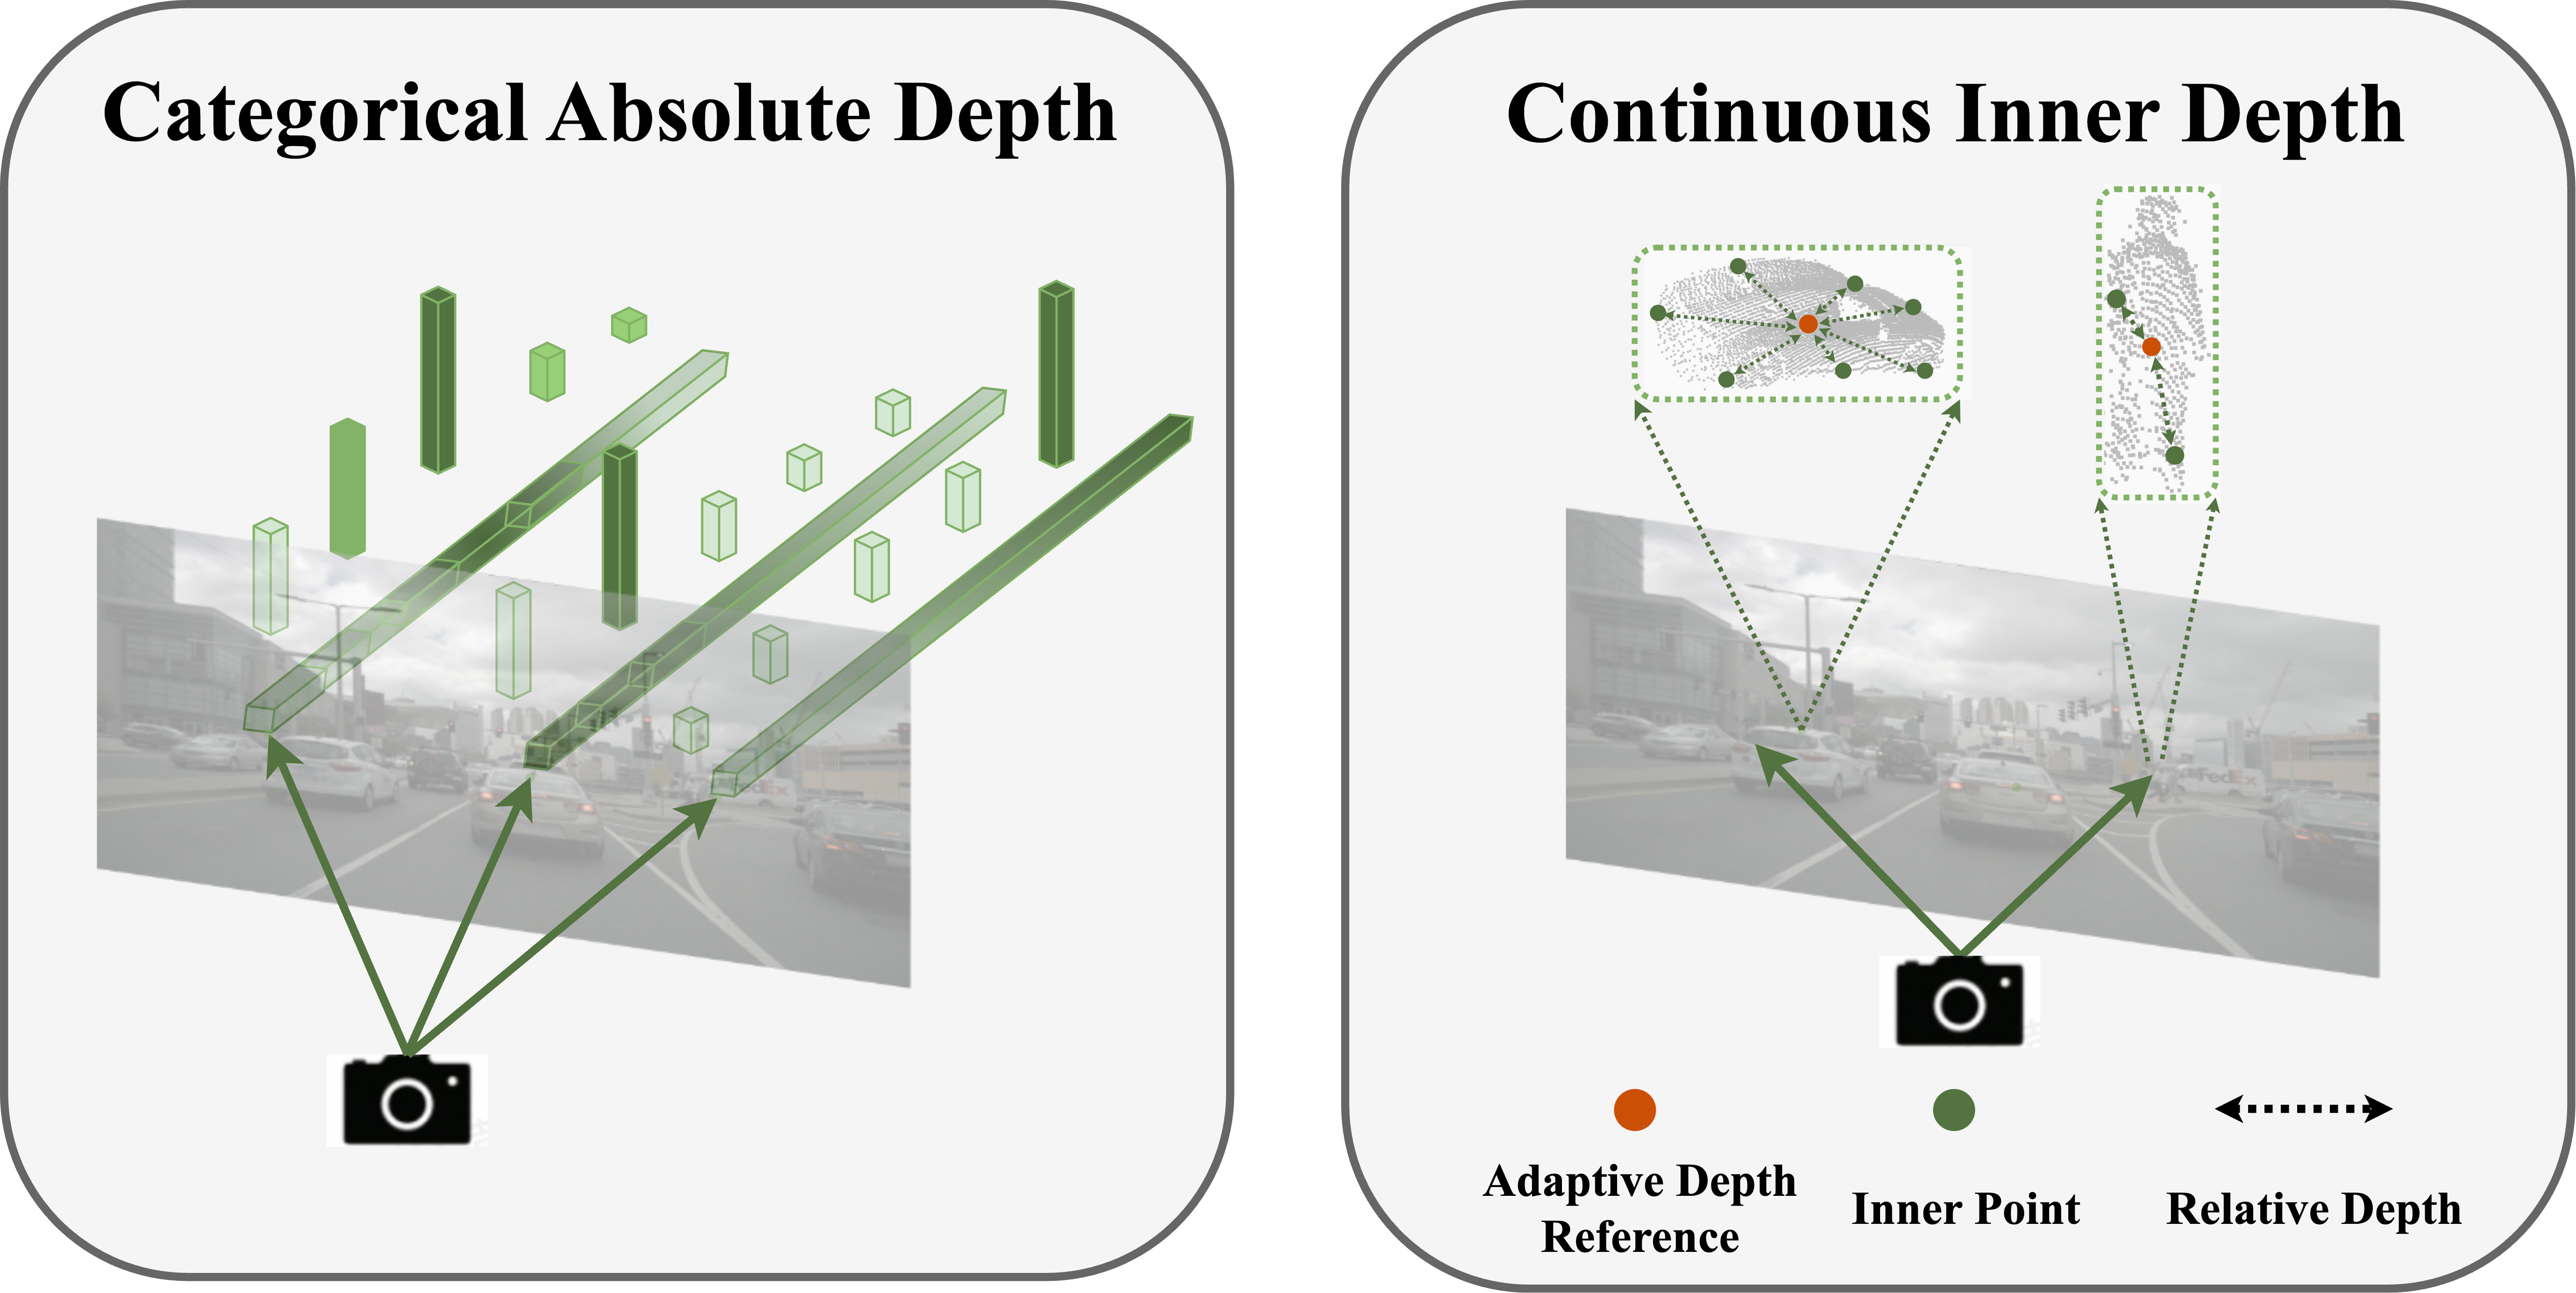
\includegraphics[scale=0.042]{cvpr_2022/iccv_fig5.drawio.png}
    \caption{\textbf{Comparison of Categorical Absolute Depth and Continuous Inner Depth.} We adopt the inner-depth supervision with continuous depth values to guide the camera-based student to learn local spatial structures of foreground object targets.
    }
    \label{fig:relative_depth}
    % \vspace{-0.8cm}
\end{figure}

%Start with $N$ ground truth 3D bounding boxes $\bm{B_{gt}}= \{\bm{b}_{i}\}_{i=1}^{N}$, which contains box center position, size and heading angle. We then obtain points in each 3D bounding boxes $\bm{P_{gt}}= \{\bm{P}^{pc}_i\}_{i=1}^{N}$, ${P}^{pc}_i$ means point clouds $P$ within 3d bounding box ${b}_{i}$. Take an object instance as example, we project ${P}^{pc}_i$ on image coordinate. 

%\begin{equation}
%    \hat{P_i^{}}(ud, vd, d) = K_{i}(R_i P_{i} + t_i),
%\end{equation}
 %In the section 3.1, we consider the depth estimation as a classification problem of the depth distribution. For the defined depth bins $b_i$, we interpret the $D$ Softmax scores, $p_k$, $k=1,..,D$, and choose the final prediction depth $b^{k}_i$ at highest prediction confidence bin. 

% In the absolute depth supervision, we apply one hot encoding to ${D_i}^{gt}$ considering the depth estimation as a classification problem of the depth distribution, first adopted in BEVDepth \cite{b7}. We divided the depth distance into D depth bins, the depth-bin-centers set denoted as ${\mathbf{B_i}=\{b^1_i, b^2_i,..., b^k_i,... b^D_i\}}$ , and we interpret the $D$ Softmax scores, $p^{k}_i$, $k=1,..,D$ at each pixel as probabilities over the ${\mathbf{B_i}}$ vector, and choose the final prediction depth $b^{k}_i$ at highest prediction confidence bin. 
%  \begin{equation}
%  \label{eq:FM}
%  \begin{aligned}
%     D_i = b^{k}_i {\max_{k=1}^D {{p^{k}_i}}}.
%  \end{aligned}
%  \end{equation}
% Here, we want to calculate the exact relative depth for different pixels within the target, the discrete depth prediction like above is not enough to express the tiny depth difference. Thus, for the further accurate prediction depth and can be used for the relative depth relation among different pixels within the certain ROI, we calculate the final depth value $\hat{D_i}$ by the hybrid mean regression as follow:
%  \begin{equation}
%  \label{eq:FM}
%  \begin{aligned}
%     {\hat{D_i}} = {\sum_{k=1}^D {{b^{k}_i}{p^{k}_i}}}.
%  \end{aligned}
%  \end{equation}
 % Compared the discrete depth prediction, we do not predict the depth as the chosen likely bin. This enables us to predict smooth depth without the discriminative artifacts, which helps to obtain the complete representation of the geometry depth.  
 
 \paragraph{Adaptive Depth Reference.}
 To calculate the relative depth values, we propose to utilize an adaptive depth reference for different foreground targets.
 Specifically, according to the predicted continuous depth values in $\{\hat{S_j}\}_{j=1}^M$, we select the pixel with the smallest depth prediction error as the reference point for each target, and correspondingly set its depth value as the depth reference, as shown in Figure~\ref{fig:relative_depth}. For the $j$-th target with the ground-truth inner-depth $\{\hat{S_j}, \hat{S^{gt}_j}\}_{j=1}^M$, we calculate the depth reference point $(x_r, y_r)$ by
  \begin{equation}
 \label{eq:FM}
 \begin{aligned}
    (x_r, y_r) = \mathop{\text{Argmin}}_{(x, y)\in \hat{S_j}} \left ({S^{gt}_j}(x, y) - {\hat{S_j}}(x, y)\right ).
 \end{aligned}
 \end{equation}
 Then, the predicted and ground-truth reference depth values are denoted as $d_j(x_r, y_r)$ and $d^{gt}_j(x_r, y_r)$, respectively. By adaptively selecting the reference point with the smallest error, the inner-depth distribution can dynamically adapt to objects with different shapes and appearances, which stabilizes the network learning for some truncated and occluded objects.

\paragraph{Inner-depth Calculation.}
On top of the reference depth value, we calculate the relative depth values within the foreground area of each target object. For pixel $(x, y)$ of the $j$-th target $\{\hat{S_j}, S_j^{gt}\}$, the predicted and ground-truth inner-depth values are formulated as
\begin{equation}
 \label{eq:FM}
 \begin{aligned}
    rd_j(x, y) &= d_j(x, y) - d_j(x_r, y_r),\\
    rd^{gt}_j(x, y) &= d^{gt}_j(x, y) - d^{gt}_j(x_r, y_r).
 \end{aligned}
 \end{equation}
 We denote the obtained relative depth-value sets for $M$ target objects as $\{\hat{R_j}, R_j^{gt}\}_{j=1}^M$. Finally, we supervise the inner-depth prediction of the student detector by an L2 loss, formulated as
 \begin{equation}
\label{eq:FM}
    \mathcal{L}_{\rm{depth}}^{R} = \sum_{j=1}^M ||\hat{R}_{j}-R^{gt}_{j}||_2.
\end{equation}
 
%  When we set the inner point and the reference point within the ROI, we can define the two relative depth sets ${\mathbf{\hat{D}}^{gt}}$ ${\mathbf{\hat{D}}^{pred}}$ of the pixels with cardinality ${M}$. 
% \begin{equation}
%     {\mathbf{\hat{D}}^{gt}} = 
% \left[{\hat{D}^{gt}_{1r},\hat{D}^{gt}_{2r},\cdots,\hat{D}^{gt}_{ir},\hat{D}^{gt}_{Mr}}\right].
% \end{equation}
% \begin{equation}
%     {\mathbf{\hat{D}}^{pred}} = 
% \left[{\hat{D}^{pred}_{1r},\hat{D}^{pred}_{2r},\cdots,\hat{D}^{pred}_{ir},\hat{D}^{pred}_{Mr}}\right].
% \end{equation}
%  where the ${\hat{D}_{ir}^{gt}}=\hat{D}_i^{gt}-\hat{D}_r^{gt}$ and ${\hat{D}_{ir}^{pred}=\hat{D}_i^{pred}-\hat{D}_r^{pred}}$ denotes the relative depth distance of the lidar pixels and cam pixels. 
 
%  To obtain the inner-geomtry depth relation from the lidar points, we minimize the discrepancy between the above sets in a one-to-one relative spatial matching manner. 
% \begin{equation}
% \label{eq:FM}
%     \mathcal{L}_{\rm{Rdepth}} = ||{\mathbf{\hat{D}}^{gt}}-{\mathbf{\hat{D}}^{pred}}||_2 = \sum_{i=1}^M ||\hat{D}^{gt}_{ir}-\hat{D}^{pred}_{ir}||_2.
% \end{equation}
%% \KY{focus on semantic mismatch}
%\noindent This formulation assumes that the semantic distributions of the teacher and the student match exactly. 
% However, a recent study~\cite{Cho2019OnTE} observes that small students are inefficient to mimic large teachers. 
%However, as mentioned earlier, for the feature maps of the teacher network, which usually encompasses more layers and larger feature channels, the spatial information of the same pixel location contains a richer semantic information compare to the student network. Directly regressing the features in a pixel-wise manner may lead to suboptimal distillation results. 
% has a stronger learning capability (\eg larger receptive field) and richer representation. That means the semantic of spatial components of teacher and student usually varies. Directly linking the teacher and student by spatial order may trigger the issues of semantic mismatch and lead to sub-optimal results.
% \KY{this is not helping the story, size difference is one reason that KD is hard. but our approach does not help in this way} 
% As the teacher grows in capacity and accuracy, the student often finds it difficult to emulate the teacher. 
% To this end, we propose to guide the whole student to mimic each spatial component of the teacher respectively. In this way, we can increase the matching capability and subsequently improve the knowledge distillation performance.

%This formulation does not consider the gap of expressivity and the exact semantic distance between $f^s_i$ and $f^t_i$, which may introduce bias. To address the limitation of Eq. \ref{eq:FM}, we reconfigure each elements in set $f^s$ by a target-aware transformer. 
%A straightforward solution is to measure the semantic distance between the elements of two sets and then assign the $f^t_i$ with the most semantic-related one from $f^s$. As we will demonstrate, this is the special case of our proposed method.
%To this end, we propose a one-to-all spatial matching knowledge distillation pipeline that allows the each feature location of the teacher to teach the entire student features in a dynamic manner.
%To make the whole student mimic a spatial component of the teacher, we propose the \textbf{T}arget-\textbf{a}ware \textbf{T}ransformer (\textbf{TaT}) to pixel-wisely reconfigure the semantic of student feature in the certain position.
%We propose the Target-aware Transformer (\textbf{TaT}) to pixel-wisely reconfigure the semantic of student feature in the certain position. 
%Given a spatial component (alignment target) of the teacher, we use \textbf{TaT} to guide the whole student to reconstruct the feature in its corresponding location. Conditioned on the alignment target,  \textbf{TaT} should reflect the semantic similarity with the components of the student feature. We use a linear operator to avoid changing the distribution of student semantics. The formulation of transformation operator $W^i$ can be defined as:
%Given the alignment target $f^t_i$, \textbf{TaT} is to find the weights $W^i$ that controls the flow of semantic aggregation across the student feature w.r.t the $i$-th pixel of student feature. Conditioned on the alignment target, \textbf{TaT} should reflect the semantic similarity with the components of the student feature. Also, it should be a linear operator otherwise it changes the distribution of student semantics. The formulation of $W^i$ can be defined as:
%\begin{equation}
%\label{eq:spe}
%\begin{aligned}
%   W^i&= \sigma(\langle {f^s_1},{f^t_i}\rangle,\langle {f^s_2},{f^t_i}\rangle,\dots,\langle {f^s_N},{f^t_i}\rangle)\\
%   &=[{w^i_1},{w^i_2},\dots,{w^i_N}],
%\end{aligned}
%\end{equation}
%\noindent where $f^t_i$ and $f^s_i$ denote the corresponding $i$-th components of teacher and student, $\langle \cdot,\cdot \rangle$ represents the inner-product and  $\|W^{i}\|=1$. We use inner-product to measure the semantic distance and softmax function for normalization. 
%Note that if we only reserve the entry of the maximum of $W^{'}$, it degrades to the nearest-neighbor. 
% Here $W^{i}$ is the gate that guides the semantic flow to the reconfigured point ${f^s_i}^{'}$. 



%Note this is the simple non-parametric method that only depends on the original features. To facilitate the training, we introduce the parametric method with the extra linear transformation applied on the student feature and teacher feature. We observe that parametric version performs better than non-parametric one in ablation study. Guided by the target-aware transformer, the reconfigured student feature can be formulated as: 
% \KY{why we need parameteric formulation? does non-param work? do we have the experiment? if not, consider to do this in supplementary}
% Also, the issue of semantic mismatching may occur in the channel dimension. To address this issue, we propose to partition the feature tensor along the channel dimension and performs the self-assembling in parallel:
%\begin{equation}
%\label{eq:mul-self-essem}
%    {f^s}^{'}=\sigma(\gamma(f^{s})\cdot \theta({f^t})^{\top})\cdot \phi(f^{s}),
%\end{equation}
%\noindent where $\theta(\cdot)$, $\gamma(\cdot)$ and $\phi(\cdot)$ are the linear functions consisting of $3\times 3$ conv layer plus the BN layer \cite{ioffe2015batch}. We compare the parametric \textbf{TaT} to non-parametric one to analyse the effectiveness brought by these linear functions in the Section~\ref{sec:ablation}. 
%In the case that the channel numbers of $F^S$ do not match with that of $F^T$, $\gamma(\cdot)$ can help with alignment.

% \KY{where? point the section} 
%The resulting \textbf{TaT} map ($\gamma(f^{s})\cdot \theta({f^t})^{\top}$) is of size $\mathbb{R}^{HW \times HW}$, which is acceptable considering that most classification networks have small feature map size on the top layers. On ResNet18, the spatial size of feature map in the 4-th block is, for example, $7\times7$.  \KY{discuss the complexity in the next section...}

%After reconfiguration, each component of ${f^s}^{'}$ aggregates the meaningful semantic from the original feature, which enhances the expressivity. We do not require the student to reconstruct the teacher feature in a pixel-to-pixel manner. Indeed, our model allows the student to act as a whole to mimic the teacher. The resulting ${f^s}^{'}$ is lately asked to minimize the L$_2$ loss with the teacher feature. The objective for \textbf{TaT} knowledge distillation can be given by:
%\begin{equation}
%    \mathcal{L}_{\rm{TaT}}= ||{f^s}^{'}-f^t||_2.
%    \label{eq:fm}
%\end{equation}

% \KY{this only apply to Cls? how about other loss? consider change cls $\rightarrow$ task. L_T -> $L_{TaT}$ }
%Finally, the total loss of our proposed method can be defined by: 

%\begin{equation}
%\label{eq:objective}
    %\mathcal{L}=\alpha\mathcal{L}_{\rm{Task}}+\beta\mathcal{L}_{\rm{KL}}+\epsilon\mathcal{L}_{\rm{TaT}},
%\end{equation}
%\noindent Here $\mathcal{L}_{\rm{Task}}$ can be any loss on the generic machine learning tasks. $\alpha$, $\beta$ and $\epsilon$ are the weight factors to balance the loss. 
%Empirically, we find that our model benefits from $\mathcal{L}_{\rm{KL}}$. However, the model can achieve state-of-the-art without the help of $\mathcal{L}_{\rm{KL}}$.
% , \ie, $\beta$ is set to 0. \KY{this is strange... why mentioning this if we set beta = 0??}

% \subsection{Empirical \& Theoretical Analysis}
% This section provides some intuition to the formulation discussed above. Without loss of generality, let's remove the linear functions $\theta(\cdot)$ and $\gamma(\cdot)$ and consider only one attention head. The Eq. \ref{eq:fm} can be expressed in another way:
% \begin{equation}
%     softmax(X\cdot Y^{\top})\cdot X=Y.
% \end{equation}
% \noindent Here $softmax(X\cdot Y)$ is the cross-attention matrix which is applied to the student feature $X$. The objective for the student is to reconstruct the teahcer feature. Denote the optimum solution to $X$ as $\hat{X}$. The non-trivial solution indeed requires that $softmax(\hat{X}\cdot Y^{\top})=I$ and $\hat{X}=Y$.

% Recall that each raw of $X$ and $Y$ corresponds to a pixel in the original feature tensor. By means of matrix multiplication, it calculates the inner-product of each paired pixels between student and teacher, resulting the cross-attention matrix. The inner-product between two pixels measures the similarity against difference, and it's normalized by the softmax function. Since the cross-attention matrix is required to be the identity matrix, this can be interpreted that the distance, reflected by the inner-product, of the associated positions between $f_s$ and $f_t$ should be as close as possible, otherwise distant. This is the necessary condition if $\hat{X}=Y$ holds.

% We now begin to give a theoretical analyse to the existence of the solution $\hat{X}$. Because student feature is expected to match the teacher feature, we have $\hat{X}=Y$. Thus, we need to prove that $softmax(Y,Y^{\top})=I$. We presume that the elements of $Y$ is Gaussian distribution and each raw is not linearly dependent from each other. Here $Y$ can be represented as:
% \begin{equation}
% \begin{aligned}
%   Y=[{y_1}^{\top},{y_2}^{\top},{y_3}^{\top},\dots,{y_N}^{\top}]^{\top},\\
% \end{aligned}
% \end{equation}
% \noindent where $Y$ has $N=H\cdot W$ raw vectors. Suppose that $y_i$ and $y_j$ are two distinct vectors, they can be described as:
% \begin{equation}
% \begin{aligned}
%   y_i=[y_{i,1},y_{i,2},y_{i,3},\dots,y_{i,C}],\\
%   y_j=[y_{j,1},y_{j,2},y_{j,3},\dots,y_{j,C}],\\
% \end{aligned}
% \end{equation}
% where $(1\leq i,j\leq N)$ and each vector is of length $C$. The expected value of the inner-product of two vectors can be given by:
% \begin{equation}
% \label{eq:in_prd_same}
%     \begin{aligned}
%       \mathbb{E}\langle y_i,y_i\rangle &= \mathbb{E}(y_{i,1}^2+y_{i,2}^2+y_{i,3}^2+\dots+y_{i,C}^2) \\
%       &=\sum_{k=1}^{C}\mathbb{E}y_{i,k}^2= \sum_{k=1}^{C}(\mu_{i,k}^2+\sigma_{i,k}^2)=C ,
%     \end{aligned}
% \end{equation}

% \begin{equation}
% \label{eq:in_prd_diff}
%     \begin{aligned}
%       \mathbb{E}\langle y_i,y_j\rangle 
%       &= \mathbb{E}(y_{i,1}\cdot y_{j,1}+y_{i,2}\cdot y_{j,2}+\dots+y_{i,C}\cdot y_{j,C}) \\
%       &=\sum_{k=1}^{C}\mathbb{E}(y_{i,k}\cdot y_{j,k})\\
%       &=\sum_{k=1}^C \left[ \mathbb{E}y_{i,k}\cdot \mathbb{E}y_{j,k}+Cov(y_{i,k},y_{j,k}) \right]  \\
%       &\leq \sum_{k=1}^{C}(\mu_{i,k}\cdot \mu_{j,k}+|\sigma_{i,k}\cdot \sigma_{j,k}|)\\
%       &=\rho \cdot C .
%     \end{aligned}
% \end{equation}
% Here $\mu=0$ and $\sigma=1$ is the mean and standard deviation of Gaussian distribution. The Eq. \ref{eq:in_prd_same} indicates the expected value of the inner-product between a vector and itself, while Eq. \ref{eq:in_prd_diff} illustrates the inner-product of two distinct vectors, which is derived by Cauchy–Schwarz inequality a.k.a covariance inequality. Here $0\leq \rho \leq 1$ and it equals to 1 if and only if two vectors are linearly dependent. Since we presume that vectors are not linearly dependent in matrix $Y$, we have $\rho<1$.

% Given Eq. \ref{eq:in_prd_same} and Eq. \ref{eq:in_prd_diff}, we consider the diagonal of the cross-attention matrix. Normalized with softmax function, the limiting condition of the $i$-th position of the $i$-th raw can be described by:
% \begin{equation}
% \label{eq:lim}
%     \lim_{C\to \infty} \frac{e^C}{(N-1)\cdot e^{\rho\cdot C}+e^C}=1.
% \end{equation}

% The limiting condition presented in Eq. \ref{eq:lim} means the $i$-th raw of the cross-attention map is the one-hot vector where $i$-th position is 1 as long as the feature channel is deep enough. Thus the resulting cross-attention matrix is an identity matrix. In our experiment setting, the feature tensor of 4-th layer in ResNet18 is of size $7\times 7 \times 512$, \ie $N=49$ and $C=512$. Even though $\rho$ reaches 0.98, Eq. \ref{eq:lim} can return 0.998 that is very close to 1.  

%--------------------------------------------------------------------------------

%--------------------------------------------------------------------------------
\subsection{Inner-feature BEV Distillation}
\label{sec:Inner-feature BEV Distillation}
%In this section we introduce the adaption of the model discussed previously and show its application on semantic segmentation. 
% \KY{inductive bias? do we really want to talk about this?}
% \ky{Although our one-to-all distillation approach can address the semantic mismatch, it has one limitation about the computational complexity. As the resulting correlation mapping }
% The proposed \textbf{TaT} lift the limitation of previous one-to-one spatial matching fashion. 
%For example, features in the neighborhood are more relevant to themselves, on the contrary, features that are farther away are less relevant. The student must figure out all of these in the learning process, which may be very challenging when the feature map is large.

Besides the depth supervision for low-level spatial information, our TiG-BEV also adopts the inner-geometry learning for high-level BEV semantics from pre-trained LiDAR-based detectors. 
Previous works~\cite{b9,b52} for BEV distillation directly force the student to imitate the teacher's features point-to-point in the BEV space. In spite of the performance improvement, such strategies are constrained by the following two aspects. On the one hand, due to the sparsity of scanned point clouds, the LiDAR-based BEV features might contain redundant and noisy information in the background areas. Although BEVDistill~\cite{b9} utilizes foreground masks to alleviate this issue, such dense feature distillation still cannot provide focused and effective guidance to the student network. On the other hand, the camera-based and LiDAR-based BEV features depict different characteristics of the scene, respectively, visual appearances and spatial structures. Therefore, forcing the BEV features to be completely consistent between two modalities is sub-optimal considering the semantic gap. In our TiG-BEV, we propose an inner-feature BEV distillation (Figure~\ref{fig:structure_attn}) consisting of inter-channel and inter-keypoint learning schemes, which conducts attentive target features distillation and relieve the cross-modal semantic gap.

% There are two main observations, on the one hand, the feature distribution of point clouds and images are not consistent due to the sparsity of point clouds, directly distilling on all region of features is not reasonable. On the other hand, even features of two modalities can hold meaningful information in the region of foreground, the representation of the features from different modalities are diverse in channel and spatial wise. Forcing students to imitate the foreground feature of the teacher is sub-optimal. Therefore, we propose a foreground structured attention feature supervision module to transfer more reliable relative spatial feature relationships from LiDAR-based teacher to multi-view based student. It contains of two distillation modules: 1) Inner Target-Aware distillation, 2) Local Target-Aware distillation,which..


\paragraph{Target Keypoint Extraction.}
To distill the knowledge of LiDAR-based detectors only within sparse foreground regions, we extract the BEV area of each object target and represent it by a series of keypoint features.
Given the ground-truth 3D bounding box for each target, we first enlarge the box size for a little bit in the BEV space to cover the entire foreground area, e.g., object contours and edges. Then, we uniformly sample its BEV bounding box by $N$ keypoints, and adopt bilinear interpolation to obtain the keypoint features from the encoded BEV representations. From both camera-based $F^{2d}_{\rm bev}$ and LiDAR-based $F^{3d}_{\rm bev}$, we respectively extract the keypoint features for all $M$ object targets as $\{f_j^{2d}, f_j^{3d}\}_{j=1}^M$, where $f_j^{2d}, f_j^{3d} \in {\mathbb{R}^{N\times C}}$. By the uniform sampling, such BEV keypoints can well represent the part-wise features and the inner-geometry semantics of foreground targets.

\begin{figure}[!t]
% \vspace{-0.5cm}
    \centering
    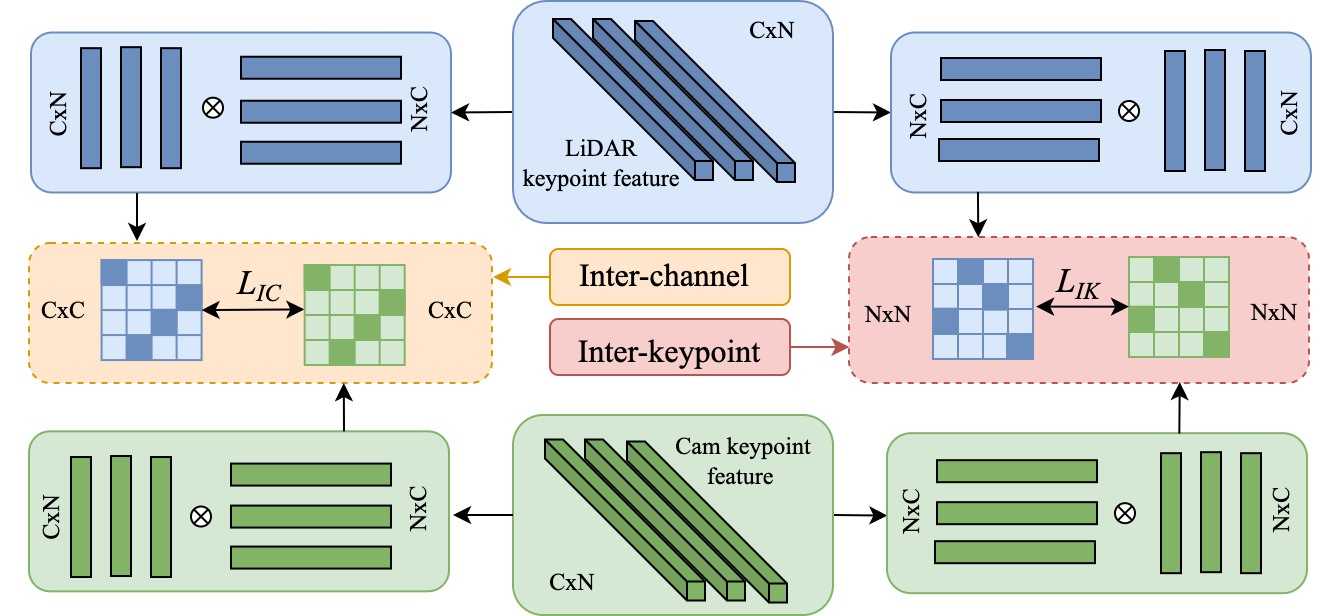
\includegraphics[scale=0.17]{cvpr_2022/iccv_fig6_2.drawio.png}
    \caption{\textbf{Detials of Innter-feature BEV Distillation.} For each foreground area in BEV space, we represent rach target feature by a set of keypoints and conduct feature distillation in both inter-channel and inter-keypoint manners.
    }
    \label{fig:structure_attn}
    % \vspace{-0.8cm}
\end{figure}

% and the corresponding background regions and divide into small grids with spatial resolution of $G_i\times G_i \times G_i$, which can summarize each foreground area into the certain number of feature keypoints.  For the bird-view feature maps, we project the keypoint $p_i$ to the 2D bird-view coordinate system and utilize bilinear interpolation to obtain the features $f^{bev}_i$ from the bird-view feature maps. Hence, the roi feature can be represented as follow:

% \begin{equation}
%     {F_i^{ROI}} = {f^{bev}_1,...,f^{bev}_i,f^{bev}_n}, 
%  i=1,..N
% \end{equation}
% which have the strong capability of preserving 3D geometry information of the foreground scene and can also boost the marginal awareness performance of the certain target.

\paragraph{Inter-channel BEV Distillation.}
% \label{sec:seq}
Taking the $j$-th object target as an example, we first apply an inter-channel BEV distillation, which guides the student keypoint features to mimic the channel-wise relationships of the teacher's. Such inter-channel signals imply the overall geometric semantics of each object target. Compared with the previous channel-by-channel supervision, our inter-channel distillation can preserve the distinctive aspects of the two modalities, while effectively transfer the well pre-trained knowledge of LiDAR-based detectors. Specifically, we calculate the inter-channel similarities of both camera-based and LiDAR-based keypoint features, formulated as
\begin{equation}
    A_j^{2d} = f_j^{2d} {f_j^{2d}}^{\top};\ \ \ A_j^{3d} = f_j^{3d} {f_j^{3d}}^{\top},
\end{equation}
where $A_j^{2d}, A_j^{3d} \in {\mathbb{R}^{C\times C}}$ denote the feature relationships between different $C$ channels for the two modalities. For all $M$ objects in a scene, we adopt L2 loss between the two inter-channel similarities for feature distillation, formulated as
\begin{equation}
    \mathcal{L}_{\rm{bev}}^{{IC}}= \sum_{j=1}^{M} ||A_j^{3d}-A_j^{2d}||_2.
    \label{eq:fm}
\end{equation}

% Given the RoI feature of each box proposal, the lidar-based bev feature and cam-based bev feature can be represented as $F_i^{Lidar}\in {\mathbb{R}^{N\times C}}$, $F_i^{cam}\in {\mathbb{R}^{N\times C}}$ respectively, where ${N}$ represents the number of keypoints and ${C}$ represents the channels numbers. For the certain sampled feature of the keypoint, it reflects the certain information within the receptive field. As mentioned before, the lidar-based detector has the better detection performance since the spatial information of the same inner roi location contains the richer semantic information compare to the cam-based detector. Thus, we propose a inner target-aware (\textbf{ITA}) distillation that performs distillation within channel wise, which allows student to learn the context of feature from RoI patches and retain the correlation among different channels. For the bev feature ${i}$th ROI, the channel-wise information matrix is defined as: 
% \begin{equation}
%     {G_i^{ROI}} = {F^{Lidar}_i\cdot {F^{Lidar}_i}}^{\top}
% \end{equation}
% The information matrix has a size of ${C\times C}$ regardless of the spatial dimension ${N}$. ${G_{i,(m,n)}^{ROI}}$ denotes the inner channel correlation between $m$th channel and $n$th channel for the same location of the $i$th ROI.

% \begin{equation}
% \begin{aligned}
% %L_{task} = &\lambda_1 L_{per}(G_s(x),G_t(x))  +\lambda_1  L_{CE}(y,\delta(z_s))\\ & + \lambda_1L_{Focal}(y,y_{out})
% %{G_{i,(m,n)}^{ROI}} = &{f^_{1,m}}{f^_{1,n}}^{\top}  +{f^_{2,m}}{f^_{2,n}}^{\top} + \dots + \\&{f^_{N,m}}\cdot {f^_{N,n}}^{\top}
% {G_{i,(m,n)}^{ROI}} = &{f^_{1,m}}\cdot {f^_{1,n}}^{\top} + {f^_{2,m}}\cdot {f^_{2,n}}^{\top}\\ & + \dots + \\{f^_{N,m}}\cdot {f^_{N,n}}^{\top}
% \end{aligned}
% \end{equation}


% For the same roi area, to make the whole cam-based detector mimic
% a spatial component of the lidar-based detector, we use the Inner-target aware operator ${G_{i,(m,n)}^{ROI}}$ to pixel-wisely reconfigure the
% semantic of cam-based feature in the certain position and transfer the channel correlation of the lidar-based feature to the cam-based feature in the certain position. Conditioned on the same roi, the ${G_{i,(m,n)}^{ROI}}$ should reflect the semantic similarity with between the components. 

% We penalize the $L_2$ distance between the channel-wise information matrix of the lidar-based detector and the cam-based detector, allowing the cam-based to obtain the similar feature diversity for the same foreground area.
% \begin{equation}
%     \mathcal{L}_{\rm{ITA}}= ||G^{Lidar}_{i,cha}-G^{cam}_{i,cha}||_2.
%     \label{eq:fm}
% \end{equation}


\begin{table*}[ht]
\centering
\caption{\textbf{Performance Comparison on nuScenes~\cite{b6} Val Set.} 'C' and 'L' denote the camera-based and LiDAR-based methods, which refer to the input data during inference. * denotes our implementation using BEVDet\cite{b19} codebase.
%using their official codes.
% We have at least 1 absolute point of performance gain against KD \cite{Hinton2015DistillingTK} on 5 out of 7 experimental settings.
}
%\vspace{-0.2cm}
\resizebox{2\columnwidth}{!}{
\tablestyle{5pt}{1.2}
\begin{tabular}{c|c|c|c|cc|ccccc}
\toprule[1.2pt]
Method          & Modality & Backbone & Resolution & mAP↑  &NDS↑& mATE↓ & mASE↓ & mAOE↓ & mAVE↓ & mAAE↓   \\ \midrule
FCOS3D\cite{b12}          & C  &ResNet-101 & 900 $\times$ 1600 & 0.343& 0.415 & 0.725 & 0.263 & 0.422 & 1.292 & 0.153  \\
PGD\cite{b17}             & C  &ResNet-101 & 900 $\times$ 1600 & 0.369& 0.428 & 0.683 & 0.260 & 0.439 & 1.268 & 0.185  \\
MonoDETR\cite{b47}             & C  &ResNet-101 & 900 $\times$ 1600 & 0.372& 0.434 & 0.676 & 0.258 & 0.429 & 1.253 & 0.176  \\
%BEVDepth-R50        & C &ResNet-50   & 256 \times 704  & 0.351 & 0.639 & 0.267 & 0.479 & 0.428 & 0.198 & 0.475 \\
% BEVDepth\cite{b7}         & C &ResNet-101  & 512 \times 1408 & 0.412 & 0.565 & 0.266 & 0.358 & 0.331 & 0.190 & 0.535 \\
DETR3D\cite{b13}          & C &ResNet-101  & 900 $\times$ 1600 & 0.303& 0.374 & 0.860 & 0.278 & 0.437 & 0.967 & 0.235  \\
PETR\cite{b21}            & C  &ResNet-101    & 512 $\times$ 1408 & 0.357 & 0.421& 0.710 & 0.270 & 0.490 & 0.885 & 0.224  \\
BEVFormer\cite{b11}       & C  &ResNet-101   & 900 $\times$ 1600 & 0.416 & 0.517& 0.673 & 0.274 & 0.372 & 0.394 & 0.198   \\
PETRv2\cite{b24}            & C  &ResNet-101    & 640 $\times$ 1600 & 0.421& 0.524 & 0.681 & 0.267 & 0.357 & 0.377 & 0.186  \\
MonoDETR-MV\cite{b48}            & C  &ResNet-101    & 640 $\times$ 1600 & 0.428 & 0.531 & 0.676 & 0.268 & 0.352 & 0.380 & 0.169  \\ \midrule
CenterPoint~\cite{b53} (Teacher)   & L &VoxelNet   & -          & 0.564 & 0.646& 0.299 & 0.254 & 0.330 & 0.286 & 0.191  \\ \midrule
BEVDet$^*$ \cite{b19} & C &ResNet-50   & 256 $\times$ 704 & 0.298& 0.379 & 0.725 & 0.279 & 0.589 & 0.860 & 0.245  \\ 
\rowcolor{gray!12} \textbf{+ TiG-BEV}     &C  &ResNet-50  & 256 $\times$ 704 & \textbf{0.331} & \textbf{0.411}& 0.678 & 0.271 & 0.589 & 0.784 & 0.218  \\ 
\rowcolor{gray!12}& &&& \textbf{\textcolor{blue}{+3.3$\%$} }& \textbf{\textcolor{blue}{+3.2$\%$}}&\textcolor{blue}{-4.7$\%$} & \textcolor{blue}{-0.8$\%$} & \textcolor{blue}{-0.0$\%$} & \textcolor{blue}{-7.6$\%$} & \textcolor{blue}{-2.7$\%$}   \\ 
\midrule
BEVDet4D$^*$ \cite{b23} & C &ResNet-50   & 256 $\times$ 704 & 0.322 & 0.451& 0.724& 0.277& 0.520 &0.366 &0.212  \\
\rowcolor{gray!12} \textbf{+ TiG-BEV}     & C &ResNet-50  & 256 $\times$ 704 & \textbf{0.356}& \textbf{0.477} & 0.648 & 0.273 & 0.517 & 0.364 & 0.210  \\ 
\rowcolor{gray!12}& &&& \textbf{\textcolor{blue}{+3.4$\%$} }& \textbf{\textcolor{blue}{+2.6$\%$}}&\textcolor{blue}{-7.6$\%$} & \textcolor{blue}{-0.4$\%$} & \textcolor{blue}{-0.3$\%$} & \textcolor{blue}{-0.2$\%$} & \textcolor{blue}{-0.2$\%$}   \\ 
\midrule
BEVDepth$^*$ \cite{b7} & C &ResNet-101   & 512 $\times$ 1408 & 0.416 & 0.521& 0.605 & 0.268 & 0.455 & 0.333 & 0.203  \\
\rowcolor{gray!12}   \textbf{+ TiG-BEV}   & C & ResNet-101  & 512 $\times$ 1408  & \textbf{0.440}& \textbf{0.544} & 0.570 & 0.267 & 0.392 & 0.331 & 0.201  \\ 
\rowcolor{gray!12}& &&& \textbf{\textcolor{blue}{+2.4$\%$} }& \textbf{\textcolor{blue}{+2.3$\%$}}&\textcolor{blue}{-3.5$\%$} & \textcolor{blue}{-0.1$\%$} & \textcolor{blue}{-6.3$\%$} & \textcolor{blue}{-0.2$\%$} & \textcolor{blue}{-0.2$\%$}   \\ 
\bottomrule[1.2pt]
\end{tabular}
}

\label{tab:nus_val_sota}
%\vspace{-3mm}
\end{table*}
\paragraph{Inter-keypoint BEV Distillation.}
\label{sec:anchor}
The inter-channel distillation guides the camera-based detector to learn the channel-wise diversity from the LiDAR-based teacher. However, it is conducted without considering the inner correlation of different keypoints within each object target, which is not capable of capturing the local geometries among different foreground parts, e.g., the front and rear of cars. To this end, we propose to utilize the inter-keypoint correlations of LiDAR-based BEV features and transfer such inner-geometry semantics into camera-based detectors. Analogous to the aforementioned inter-channel module, for the $j$-th target object, we calculate the inter-keypoint similarities in a transposed manner for the two modalities as
\begin{equation}
    B_j^{2d} = {f_j^{2d}}^{\top} {f_j^{2d}};\ \ \ B_j^{3d} = {f_j^{3d}}^{\top} {f_j^{3d}},
\end{equation}
where $B_j^{2d}, B_j^{3d} \in {\mathbb{R}^{N\times N}}$ denote the feature relationships between different $N$ keypoints respectively for camera and LiDAR. We also adopt L2 loss for all $M$ targets as
\begin{equation}
    \mathcal{L}_{\rm{bev}}^{{IK}}= \sum_{j=1}^{M} ||B_j^{3d}-B_j^{2d}||_2.
    \label{eq:fm}
\end{equation}
Then, the distillation loss for inter-channel and inter-keypoint features in BEV space is formulated as
\begin{equation}
    \mathcal{L}_{\rm{bev}}=
    \mathcal{L}_{\rm{bev}}^{{IC}}+
    \mathcal{L}_{\rm{bev}}^{{IK}},
    \label{eq:seg}
\end{equation}
where the two terms are orthogonal respectively for the channel-wise feature diversity and keypoint-wise semantic correlations.

% The attempt to preserve the local correlation through concatenating all the position would fail. 
% We hope that detector can capture the context from the one position to another within the target area. In this case, the cam-based detector will, however, be distracted from the locality since the \textbf{ITA} encodes all the related semantic over the whole feature among different positions. In other words, the \textbf{ITA} will aggregates redundant local semantic.
% Furthermore, a large feature map will hinder the inductive bias since it may encourage the student to integrate the less relevant semantic from remote positions by mistake, which may deteriorate the subsequent distillation performance.
% For complex scenes and similar targets, the postion wise dependency is important to capture the relation (\eg layout) of different components within the target.

% We address the conundrum by the proposed local target-aware(\textbf{LTA}) distillation. Like the the channel-wise information matrix defined in \textbf{ITA}, the position-wise matrix is defined as follow:
% \begin{equation}
%     {G_{i}^{pos}} = {{F^{Lidar}_i}^{\top}\cdot F^{Lidar}_i}
% \end{equation}

% The information matrix has the size of ${N\times N}$ regardless of the channel dimension ${C}$. ${G_{i,(p,q)}^{pos}}$ denotes the inner spatial correlation between $p$th keypoint and $q$th keypoint for the $i$th ROI. Similarly, the formulation of the operator can be defined as:

% \begin{equation}
% \begin{aligned}
%     {G_{i,(p,q)}^{pos}} = {f^_{p,1}}\cdot {f^_{q,1}}^{\top} + {f^_{p,2}}\cdot {f^_{q,2}}^{\top} + \dots + \\{f^_{p,C}}\cdot {f^_{q,C}}^{\top}
% \end{aligned}
% \end{equation}

% After reconfiguration, the spatial relationship within the target can be extracted and summerized, which is complementary to the channel relationship. Therefore, as the cam-based detector, we enhance its gemetry expressivity by asking them to mimic the teacher. Thus, the objective for (\textbf{LTA}) knowledge distillation can be given by:

% \begin{equation}
%     \mathcal{L}_{\rm{LTA}}= ||G^{Lidar}_{i, pos}-G^{Cam}_{i, pos}||_2.
%     \label{eq:fm}
% \end{equation}

\subsection{Overall Loss}
\label{sec:overall_loss}
To sum up, we benefit the student camera-based detector by target inner-geometry from two complementary aspects, i.e., an inner-depth supervision for low-level signals and an inner-feature BEV distillation for high-level semantics. They produce two losses as $\mathcal{L}^R_{\rm{depth}}$ and $\mathcal{L}_{\rm{bev}}$. Together with the original two losses, i.e., dense absolute depth supervision $\mathcal{L}^A_{\rm{depth}}$, and 3D detection $\mathcal{L}_{\rm{det}}$, the overall loss of our TiG-BEV is formulated as
\begin{equation}
    \mathcal{L}_{\rm{TiG}}=
    \mathcal{L}_{\rm{det}}+
    \mathcal{L}^A_{\rm{depth}}+
    \mathcal{L}^R_{\rm{depth}}+
    \mathcal{L}^{IC}_{\rm{bev}}+
    \mathcal{L}^{IK}_{\rm{bev}}.
    \label{eq:seg}
\end{equation}

% The inner target-aware distillation enables the detector to mimic the inner feature diversity while the local target-aware distillation allows it to learn the local representation over the spatial feature, which are complementary to each other. Therefore, the combination of these two objectives can bring the best of two worlds. Our objective designed for structured attention feature supervision can be written by:
% \begin{equation}
%     \mathcal{L}_{\rm{SAF}}=
%     \delta\mathcal{L}_{\rm{ITA}}+
%     \zeta\mathcal{L}_{\rm{LTA}}
%     \label{eq:seg}
% \end{equation}



% Finally, the total loss of our proposed method can be defined by:
% \begin{equation}
%     \mathcal{L}_{\rm{TiG}}=
%     \mathcal{L}_{\rm{det}}+
%     \mathcal{L}^A_{\rm{depth}}+
%     \mathcal{L}^R_{\rm{depth}}+
%     \mathcal{L}^{IC}_{\rm{bev}}+
%     \mathcal{L}^{IK}_{\rm{bev}}
%     \label{eq:seg}
% \end{equation}
% Here $L_{task}$ is the loss of the 3D detection task. $\alpha$, $\beta$, $\gamma$, $\delta$ and $\zeta$ are the weight factors to balance the loss.


\section{Experiments}

\subsection{Communication Efficiency at Scale}\label{sect:experiments_square_cube}

Before we can meaningfully evaluate SWARM parallelism, we must verify our theoretical observations on communication efficiency. Here we run several controlled experiments that measure the GPU utilization and network usage for different model sizes, using the Transformer architecture~\citep{transformer} that has been widely adopted in various fields~\citep{lin2021survey}. To decouple the performance impact from other factors, we run these experiments on homogeneous V100 GPU nodes that serve one pipeline stage over the network with varying latency and bandwidth. We use a batch size of 1 and sequences of 512 tokens; the complete configuration is deferred to Appendix~\ref{appendix:detailed_setup}.


First, we measure how the model size affects the computation to communication ratio at 500 Mb/s network bandwidth in both directions. We consider 4 model configurations: the base configuration from the BERT paper~\citep{bert}, ``xxlarge" (``large'' with $d_{model}{=}4096$),  which is used in several recent works~\citep{albert,ernie3,deberta}, and a GPT-3-scale model with $d_{model}{=}12288$~\citep{gpt3}. We also evaluate a modified Transformer architecture (``Ours'') as defined in Section~\ref{sect:experiments_large} with $d_{model}{=}4096$, 3 layers per pipeline stage and 8-bit quantized activations. As we demonstrate in Appendix~\ref{appendix:compression}, this compression strategy can significantly reduce network usage with little effect on convergence. In the first three configurations, the model consists of 12 Transformer layers placed on 12 servers with a single GPU; in the last one, there are 4 servers, each hosting 3 layers.
Appendix~\ref{appendix:detailed_setup} contains FLOP and parameter counts of each configuration.




\begin{figure}[b]
\vspace{-14pt}
    \centering
    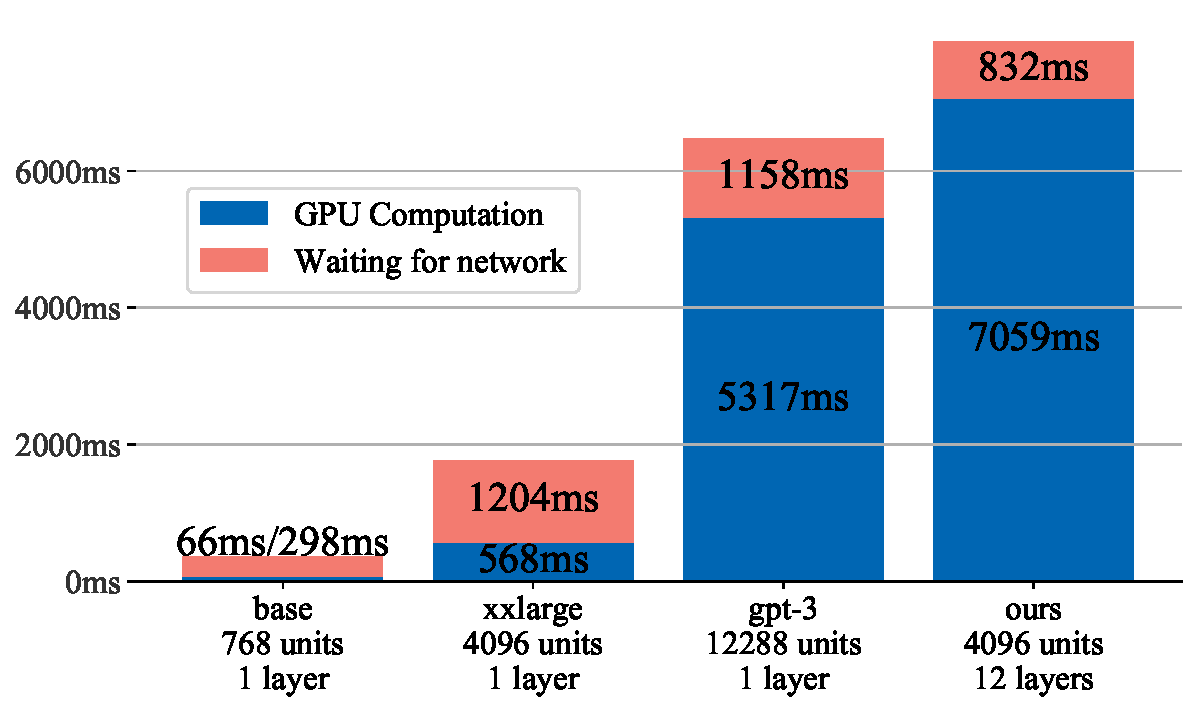
\includegraphics[width=1\linewidth]{resources/perf_absolute.pdf}
    \vspace{-12pt}
    \captionof{figure}{Pipeline computation and idle time per batch at 500 Mb/s bandwidth.}
    \label{fig:throughput_exps}
\end{figure}%
\begin{table}
    \centering
    \captionof{table}{Relative device utilization at 500 Mb/s bandwidth and varying network latency.}
    \label{tab:latency}
    \small
    \setlength{\tabcolsep}{8pt}
    \begin{tabular}[b]{@{}lcccc@{}}
    \toprule
    \multirow{2}{*}{\thead{Latency\\(RTT)}} & 
    \multicolumn{4}{c}{
    \thead{
    Relative GPU utilization\\ (100\% - idle time)
    }
    }
    
    \\
\cmidrule{2-5}                     & base & xxlarge & GPT-3 & Ours \\ \midrule
    None &   18.0\%     &  32.1\%         &  82.1\%  &  89.5\%      \\
    10ms &   11.8\%      &   28.9\%    &   79.3\%   &  87.2\%    \\
    50ms &    4.88\%      &   20.1\%    &   70.3\% &  79.5\%    \\
    100ms &    2.78\%      &    14.9\%    &  60.2\%     &   71.5\% \\
    200ms &   1.53\%     &  10.1\%    &  48.5\%   &     59.2\%    \\
    \bottomrule
    \end{tabular}
    \vspace{-6pt}
\end{table}

As depicted in Figure~\ref{fig:squarecube} (right) and Figure~\ref{fig:throughput_exps}, larger models achieve better GPU utilization rate in the same network conditions, since their communication load grows slower than computation. More importantly, even at 500 Mb/s, the resulting GPU idle time can be pushed into the 10--20\% range, either naturally for GPT-3-sized models or through activation compression for smaller models. In addition, large models maintain most of their training efficiency at the 100ms latency~(Table~\ref{tab:latency}), which is roughly equivalent to training on different continents~\citep{verizon_latency}.

\vspace{-4pt}
\subsection{Detailed Performance Comparison}\label{appendix:training_throughput}

Here we investigate how SWARM parallelism compares to existing systems for training large models: \textbf{GPipe}~\citep{huang2019gpipe} and \textbf{ZeRO-Offload}~\citep{zerooffload}.
The purpose of this section is to compare the training throughput in ``ideal'' conditions (with homogeneous reliable devices and balanced layers), as deviating from these conditions makes it \textit{infeasible} to train with baseline systems.
Still, even in such conditions the performance of different systems can vary across model architectures, and hence we want to identify the cases in which using SWARM is preferable to other approaches.
We benchmark individual SWARM components in preemptible setups in Section~\ref{sect:experiments_adaptive} and Appendix~\ref{appendix:scaling}.

We evaluate training performance for sequences of 4 Transformer layers of identical size distributed over 16 workers. Similarly to Section~\ref{sect:experiments_square_cube}, we use three layer configurations: ``xxlarge''~($d_{model} {=} 4096$, $d_{\text{FFN}} {=} 16384$, 32 heads), ``GPT-3''~($d_{model} {=} 12288$, $d_{\text{FFN}} {=} 49152$, 96 heads), and ``Ours''~($d_{model} {=} 4096$, $d_{\text{FFN}} {=} 16384$, 32 heads, 16 shared layers per block, last stage holds only the vocabulary projection layer). The microbatch size is 4 for ``xxlarge'' and 1 for ``GPT-3'' and ``Ours'', and the sequence length is 512.

To provide a more detailed view of the training performance, we measure two separate performance statistics: the training throughput and the All-Reduce time. 
The training throughput measures the rate at which the system can process training sequences, i.e., run forward and backward passes. 
More specifically, we measure the time required to process 6250 sequences of 512 tokens, which corresponds to the largest batch size used in~\citet{gpt3}.
In turn, the All-Reduce time is the time each system spends to aggregate accumulated gradients across devices. 
Intuitively, training with small batch sizes is more sensitive to the All-Reduce time (since the algorithm needs to run All-Reduce more frequently) and vice versa.


\textbf{Hardware setup:} Each worker uses a V100-PCIe GPU with 16 CPU threads (E5 v5-2660v4) and 128 GB RAM. The only exception is for ZeRO-Offload with ``GPT-3'' layers, where we had to double the RAM size because the system required 190 gigabytes at peak. Similarly to Section~\ref{sect:experiments_square_cube}, each worker can communicate at a 500 Mb/s bandwidth for both upload and download for a total of 1 Gb/s.
In terms of network latency, we consider two setups: with \textbf{no latency}, where workers communicate normally within the same rack, and with \textbf{latency}, where we introduce additional $100\pm50$ms latency directly in the kernel\footnote{More specifically, \texttt{tc qdisc add dev <...> root netem delay 100ms 50ms}}.

\textbf{GPipe configuration:} We use a popular PyTorch-based implementation of GPipe\footnote{The source code is available at \url{https://github.com/kakaobrain/torchgpipe}}. The model is partitioned into 4 stages repeated over 4 model-parallel groups. To fit into the GPU memory for the ``GPT-3'' configuration, we offload the optimizer into RAM using ZeRO-Offload. Before averaging, we use PyTorch's built-in All-Reduce to aggregate gradients.
We evaluate both the standard GPipe schedule and the 1F1B schedule~\citep{pipedream}.

\textbf{ZeRO-Offload configuration:} Each worker runs the entire model individually, then exchanges gradients with peers. For ``xxlarge'', we use the official implementation from~\cite{zerooffload}. However, for ``GPT-3'', we found that optimizer offloading still does not allow us to fit 4 layers into the GPU. For this reason, we also offload the model parameters using the \texttt{offload\_param} option.

\begin{table}
\centering
\small
\setlength{\tabcolsep}{4pt}
\captionof{table}{Training performance for different model sizes.}
\label{tab:throughput_gpt}
\begin{tabular}[b]{lcccc}
\toprule
\multirow{2}[2]{*}{System} &
  \multicolumn{2}{c}{Throughput, min/batch} &
  \multicolumn{2}{c}{All-Reduce time, min} \\ \cmidrule(lr){2-3}\cmidrule(lr){4-5} 
                 & No latency & Latency & No latency & Latency \\
 \midrule \multicolumn{5}{c}{``GPT-3'' (4 layers) }\\
 \midrule
SWARM            &  168.3 &\textbf{186.7}  &  7.4 & \textbf{7.6}   \\
GPipe            &  164.5 & 218.4 &  \multirow{2}{*}{\textbf{6.7}}    & \multirow{2}{*}{7.8}   \\
1F1B & \textbf{163.3} & 216.1 & & \\
Offload          &  272.7 & 272.7          &  25.5 & 27.3 \\
\midrule \multicolumn{5}{c}{``xxlarge'' (4 layers) }\\
\midrule
SWARM            &  44.2 & 48.2                  &  0.8  & \textbf{0.9}   \\
GPipe            &  40.1 & 108.8                  &  \multirow{2}{*}{\textbf{0.7}}  & \multirow{2}{*}{1.1}   \\
1F1B & 40.8 & 105.5 & & \\
Offload          &  \textbf{33.8} & \textbf{33.8}  &  2.8 & 4.2   \\
\midrule \multicolumn{5}{c}{Full ``Ours'' model (48 shared layers + embeddings) }\\
\midrule
SWARM            &  432.2 & 452.9                  &  0.8  &\bf 1.0   \\
GPipe            &  420.0 & 602.1                   &  \multirow{2}{*}{\bf 0.7}  & \multirow{2}{*}{1.1}   \\
1F1B             &  408.5 & 569.2 & & \\
Offload          &  \bf 372.0 &\bf 372.0  &  3.2 & 4.8   \\
\bottomrule
\end{tabular}
\vspace{-8pt}
\end{table}%

\begin{figure}[b]
\vspace{-16pt}
\centering
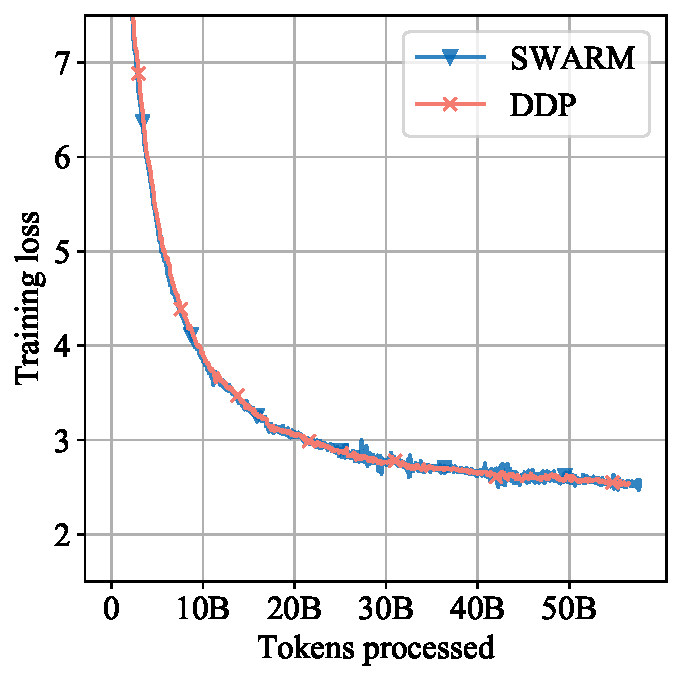
\includegraphics[ width=0.65\linewidth]{resources/learning_3stages.pdf}
\vspace{-6pt}
\captionof{figure}{Training convergence comparison.}
\label{fig:convergence}
\end{figure}

In turn, when training smaller models, ZeRO-Offload outperforms both SWARM and GPipe. This result aligns with our earlier observations in Figure~\ref{fig:squarecube}, where the same model spent most of the time waiting for the communication between pipeline stages.%

We also observe that ZeRO-Offload takes longer to aggregate gradients, likely because each peer must aggregate the entire model, whereas in SWARM and GPipe, peers aggregate a single pipeline stage. The variation between All-Reduce time in GPipe and SWARM is due to implementation differences. Overall, SWARM is competitive to HPC baselines even in an idealized homogeneous environment.

\subsection{Large-Scale Distributed Training}
\label{sect:experiments_large}

To verify the efficiency of SWARM parallelism in a practical scenario, we conduct a series of large-scale distributed experiments using preemptible (unreliable) cloud T4 and A100 GPUs over a public cloud network.

We train a Transformer language model with the architecture similar to prior work~\citep{gpt3,gptj,gptneo} and 1.01 billion parameters in total. Our model consists of 3 stages, each containing a single Transformer decoder block with $d_{model}=4096$ and 16 layers per pipeline stage. All workers within a stage serve the same group of layers, and all layers within each group use the same set of parameters, similarly to ALBERT~\citep{albert}. On top of this, the first stage also contains the embedding layer, and the last stage includes the language modeling head. Because of layer sharing, this model is equivalent to a 13B model from~\citet{gpt3} in terms of compute costs. 

We use 8-bit compression~\citep{adam8bit} for activations and gradients to reduce the communication intensity. Additional training setup details are covered in Appendix~\ref{appendix:detailed_large}.
SWARM nodes run rebalancing every $T=300$ seconds, and trainers measure peer performance using a moving average with $\alpha=0.1$. However, as we show in Section~\ref{sect:experiments_adaptive}, the throughput of SWARM is not very sensitive to the choice of these hyperparameters.



First, to verify that model parallelism with asynchronous updates does not have significant convergence issues, we train the model on the Pile~\citep{gao2020pile} dataset with 400 preemptible T4 instances, each hosting one accelerator. As a baseline, we use regular data-parallel training with offloading on 128 A100 GPUs.
We run both experiments for approximately 4 weeks and compare the learning curves.




Figure~\ref{fig:convergence} shows the results of this experiment: it can be seen that the training dynamics of two approaches are indeed similar, which demonstrates the viability of SWARM parallelism for heterogeneous and poorly-connected devices.

In the next experiment, we aim to measure the pipeline throughput in different hardware conditions and to compare it with an estimate of best-case pipeline performance.
We consider several setups: first, we use the same 400 preemptible T4 nodes; in another setup, we use 7 instances with 8 A100 GPU each; finally, we combine these fleets to create a heterogeneous setup. We examine the performance of the pipeline both with weight sharing and with standard, more common, Transformer blocks.

\begin{table}
\centering
\captionof{table}{Pipeline throughput, layer sharing.}
\label{tab:throughput}
\small
\begin{tabular}{@{}lcccc@{}}
\toprule
\multirow{2}{*}{\begin{tabular}[c]{@{}l@{}}Hardware\\ setup\end{tabular}} &
  \multicolumn{2}{c}{\begin{tabular}[c]{@{}c@{}}Throughput,\\ samples/s\end{tabular}} &
  \multicolumn{2}{c}{\begin{tabular}[c]{@{}c@{}}Optimal\\ bandwidth, Mb/s\end{tabular}} \\ \cmidrule(lr){2-3}\cmidrule(lr){4-5} 
                 & Actual & Best-case & Upload & Download \\ \midrule
T4           &  17.6      &   19.2        &   317.8     &     397.9     \\
A100          & 16.9       &   25.5        &   436.1     &     545.1     \\
T4 \& A100 &   27.3     &       ---    &   ---     &      ---    \\ \bottomrule
\end{tabular}
\end{table}
\begin{table}
\centering
\captionof{table}{Pipeline throughput, default Transformer.}
\label{tab:throughput_standard}
\small
\begin{tabular}{@{}lcc@{}}
\toprule
\multirow{2}{*}{\begin{tabular}[c]{@{}l@{}}Hardware\\ setup\end{tabular}} &
  \multicolumn{2}{c}{\begin{tabular}[c]{@{}c@{}}Throughput,\\ samples/s\end{tabular}} \\ \cmidrule(lr){2-3}
                 & Actual & Best-case \\ \midrule
T4           &  8.8      &   19.3        \\
A100          & 8.0       &   25.1        \\
T4 \& A100 &   13.4     &       ---    \\ \bottomrule
\end{tabular}
\end{table}






We measure the number of randomly generated samples processed by the pipeline both in our infrastructure and the ideal case that ignores all network-related operations (i.e., has infinite bandwidth and zero latency). The ideal case is emulated by executing a single pipeline stage 3 times locally on a single server and multiplying the single-node estimates by the number of nodes.

As demonstrated in the left two columns of Table~\ref{tab:throughput} and Table~\ref{tab:throughput_standard}, asynchronous training of compute-intensive models with 8-bit compressed activations regardless of the architecture specifics allows us to achieve high performance without a dedicated networking solution. Furthermore, the load balancing algorithm of SWARM allows us to dynamically and efficiently utilize different hardware without being bottlenecked by slower devices. 


Next, we use the same load testing scenario to estimate the bandwidth required to fully utilize each device type in the above infrastructure. For this, we measure the average incoming and outgoing bandwidth on the nodes that serve the intermediate stage of the pipeline. We summarize our findings in the right two columns of Table~\ref{tab:throughput}: it turns out that with layer sharing and 8-bit compression, medium-performance GPUs (such as T4) can be saturated even with moderate network speeds. Based on our main experiment, the optimal total bandwidth is roughly 100Mb/s higher than the values reported in Table 3 due to gradient averaging, loading state from peers, maintaining the DHT and streaming the training data.
Although training over the Internet with more efficient hardware might indeed underutilize the accelerator, this issue can be offset by advanced compression strategies such as compression-aware architectures or layer sharing, as shown in Table~\ref{tab:throughput}.

\begin{figure}[t]
    \centering
    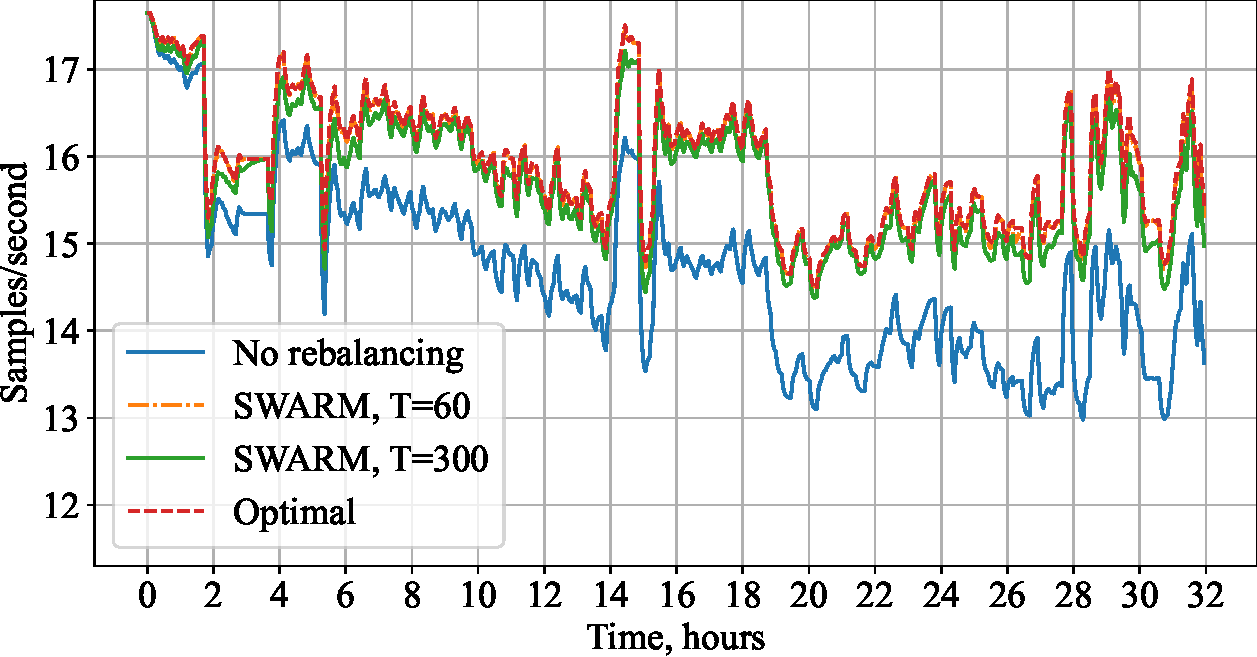
\includegraphics[width=\linewidth]{resources/rebalancing_activity.pdf}
    \captionof{figure}{Throughput of rebalancing methods over time.}
    \label{fig:rebalancing}
\end{figure}

\subsection{Adaptive Rebalancing Evaluation}


\begin{figure*}[h!]
\begin{subfigure}{0.5\textwidth}
    \centering
    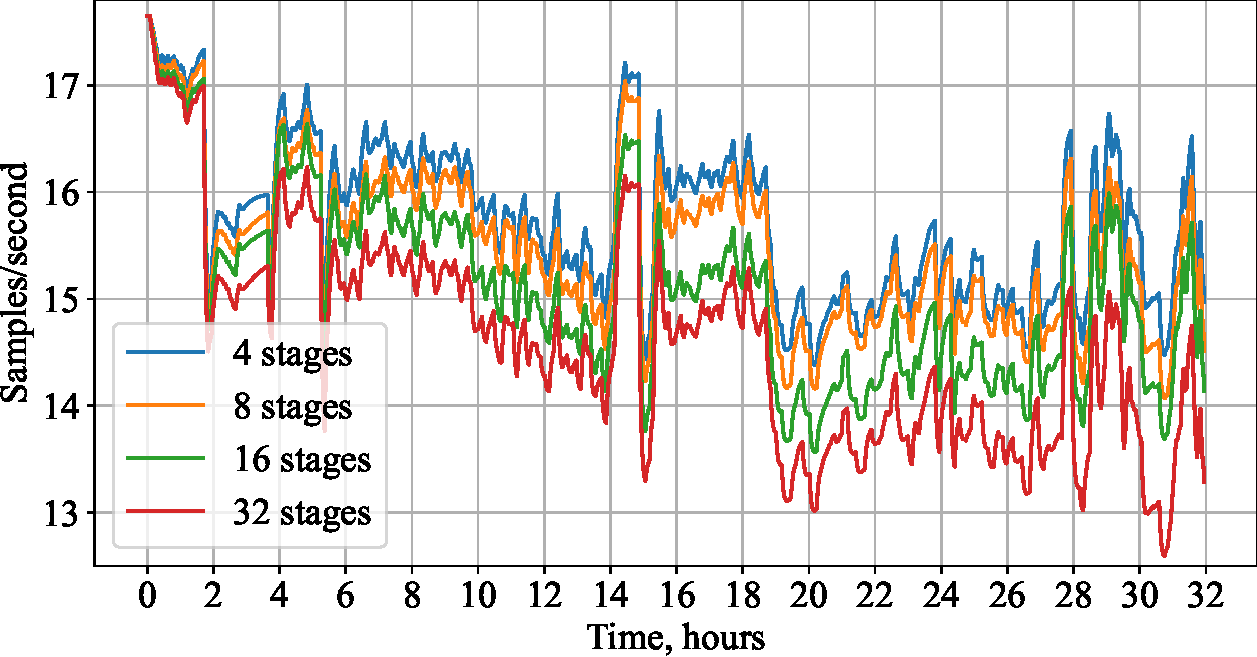
\includegraphics[width=0.97\linewidth]{resources/rebalancing_stages.pdf}
    \caption{Adaptive rebalancing of SWARM parallelism.}
    \label{fig:rebalancing_stages}
\end{subfigure}%
\begin{subfigure}{0.5\textwidth}
    \centering
    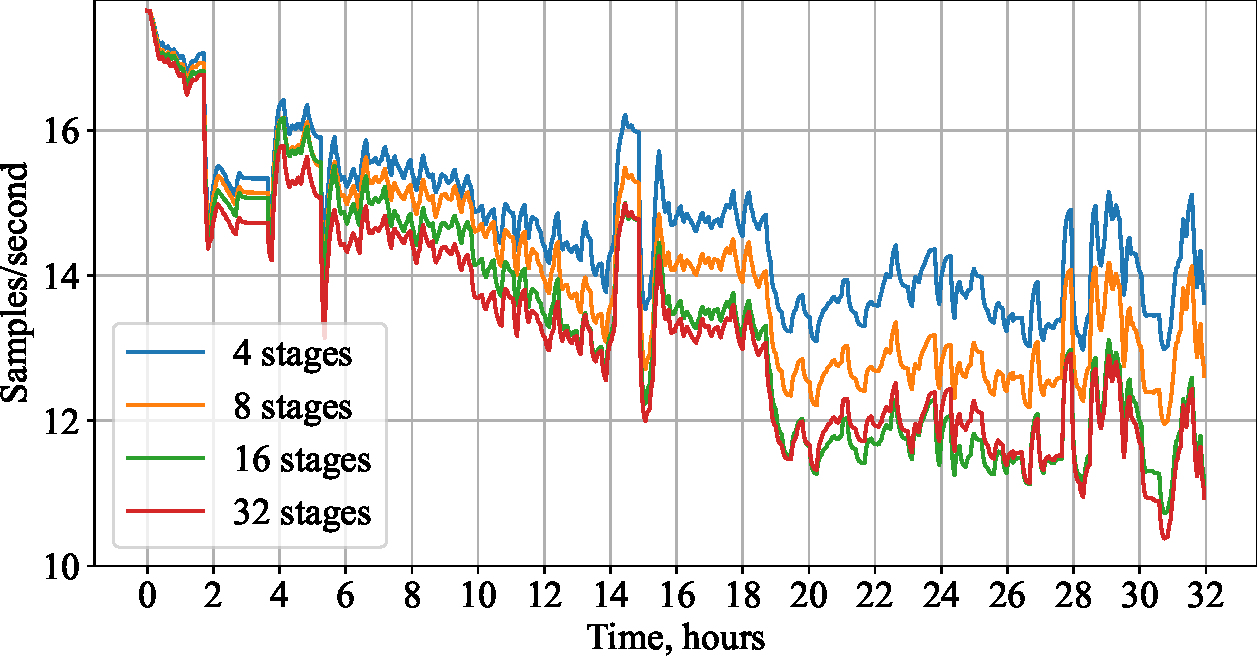
\includegraphics[width=0.97\linewidth]{resources/rebalancing_stages_baseline.pdf}
    \caption{No rebalancing.}
    \label{fig:rebalancing_stages_baseline}
\end{subfigure}
\caption{Scaling of pipeline-parallel strategies with respect to the number of stages.}
\label{fig:rebalancing_stages_all}
\end{figure*}

\label{sect:experiments_adaptive}
In this experiment, we evaluate the efficiency of adaptive peer rebalancing between stages proposed in Section~\ref{sect:method_swarm}. 
We use statistics of the number of active T4 nodes from the 32-hour segment of the experiment described in Section~\ref{sect:experiments_large}. 
We use this data to simulate training dynamics by viewing it as sequence of events, each consisting of a timestamp and a change in the number of peers (which can be positive or negative). 
When a worker is removed from the pipeline, we randomly choose the stage it was removed from: that is, removing $N$ peers corresponds to $N$ samples from the uniform distribution over four pipeline stages. 
We run 10 simulations with different random seeds and average the resulting trajectories.
We compare our strategy with two different values of $T$ to the baseline that has no rebalancing.

The results of this evaluation are available in \autoref{fig:rebalancing}; for reference, we also provide the performance of a theoretically optimal rebalancing strategy that maintains the highest possible throughput at every moment. It can be seen that even with the rebalancing period $T=300$, our approach significantly improves the overall throughput of the pipeline. When the number of peers is relatively stable, the rebalanced pipeline also approaches the optimal one in terms of throughput, which shows the efficiency of rebalancing even when moving only one node at a time.

In addition, we observed that for some brief periods, the performance of the unbalanced pipeline exceeded the throughput of the balanced one due to random choice of disconnecting peers (dropping more from the ``overrepresented'' stages affects the imbalanced pipeline less). However, this held true only for $\approx 4.5\%$ of the experiment and was quickly mitigated by adaptive rebalancing.

As expected, decreasing $T$ from 300 to 60 seconds improves both the overall throughput and the speed of convergence to optimal pipeline performance. However, the effect is not as drastic compared to the increase in DHT data transfer volume. This is also demonstrated by \autoref{tab:rebalancing_speedup}, which shows the relative throughput of the three configurations compared to the optimal one. Furthermore, the table displays that while initially there is little difference between rebalancing choices, it becomes more pronounced later on as the imbalanced version ``drifts further'' from the optimal state.

\begin{table}[b]
\centering
\captionof{table}{Relative throughput comparison of pipeline rebalancing methods.}
\small
\label{tab:rebalancing_speedup}
\begin{tabular}[b]{@{}lccc@{}}
\toprule
\multirow{2}[2]{*}{\thead{Rebalancing}} & \multicolumn{3}{c}{\% of optimal} \\ \cmidrule(l){2-4} 
                        & Overall   & First 1 hour   & Last 1 hour  \\ \midrule
None                & 82.7      & 99.0       & 45.4     \\
$T=300$    & 95.8      & 99.4       & 88.9     \\
$T=60$     & 97.6      & 99.8       & 91.7     \\ \bottomrule
\end{tabular}
\end{table}

Finally, we analyze the scaling properties of rebalancing with respect to the number of stages. To do this, we conduct experiments in the same setup as above ($T=300$) while changing the number of pipeline stages from 4 to $\{4,\ 8,\ 16,\ 32\}$. To ensure the consistency of throughput across all experiments, we increase the starting number of peers accordingly while keeping the preemption rate constant. As a baseline, we also evaluate the throughput of the pipeline that has no rebalancing.

Figure~\ref{fig:rebalancing_stages_all} shows the outcome of this experiment. As displayed in the plots, both strategies drop in performance with the increase in the stage count: while all stages should drop in performance equally in expectation, in practice, the variances are too large while the number of peers is relatively too small for the asymptotic properties to take place. This effect results in more outliers (large drops in the number of peers) in the preemption distribution for more stages. Still, rebalancing allows to partially mitigate the issue: while we observe a more consistent downward trend for the baseline strategy, the rebalanced pipeline regains its performance over time and achieves a higher overall throughput.



\section{Conclusion}
In this work, we advance the method of {machine unlearning} through a novel viewpoint: model sparsification, achieved by weight pruning. We show in both theory and practice that model sparsity plays a foundational and crucial role in closing the gap between exact unlearning and existing approximate unlearning methods. Inspired by that, we propose two new unlearning paradigms,  `prune first, then unlearn' and `sparsity-aware unlearn', which can significantly improve the efficacy of approximate unlearning. We demonstrate the effectiveness of our findings and proposals in extensive experiments across different unlearning setups. Our study also indicates the presence of \textit{model modularity} traits, such as weight sparsity, that could simplify the process of machine unlearning. This may open up exciting prospects for future research to investigate unlearning patterns within weight or architecture space.






% \bibliography{iclr2023_conference}
\bibliography{zotero,extra}
\bibliographystyle{iclr2023_conference}

\newpage


% \setcounter{lemma}{0}
%     \renewcommand{\thelemma}{\Alph{section}\arabic{lemma}}
    
\begin{comment}
\end{comment}

{\colorred 
\section{Compatible Value Function}
\label{app:comp_v}

The original policy gradient with compatible value function is stated as follow. 
\begin{theorem}
[\cite{sutton1999policy}]
Let $Q_w$ be a state-action function with parameter $w$ and $\pi_\theta$ be a policy function with parameter $\theta$. 
If $Q_w$ satisfies $\mathbb{E}_{\pi} [(Q^\pi - Q_w) \nabla_w Q_w] = 0$ and 
$\nabla_w Q_w = \nabla_\theta \log \pi_\theta,$
then $$\nabla_\theta \mathcal{J} = \mathbb{E}_\pi [Q_w \nabla_\theta \log \pi_\theta].$$
\label{thm:pg_fa}
\end{theorem}
If we let $w = \theta$ in Theorem \ref{thm:pg_fa}, where $Q_w$ and $\pi_\theta$ share parameters, we have the following theorem. 
\begin{theorem}
Let $Q_\theta$ be a state-action function with parameter $\theta$ and $\pi_\theta$ be a policy function with parameter $\theta$. 
If $Q_\theta$ satisfies $\mathbb{E}_{\pi} [(Q^\pi - Q_\theta) \nabla_\theta Q_\theta] = 0$ and 
$\nabla_\theta Q_\theta = \nabla_\theta \log \pi_\theta,$
then $$\nabla_\theta \mathcal{J} = \mathbb{E}_\pi [Q_\theta \nabla_\theta \log \pi_\theta].$$
\label{thm:pg_fa2}
\end{theorem}
Define 
$$\chi \overset{def}{=} \mathbb{E}_\pi [\cos <\nabla_\theta Q_\theta, \nabla_\theta \log \pi_\theta>].$$
We show that $\chi = 1$ is the necessary condition for the compatible condition $\nabla_\theta Q_\theta = \nabla_\theta \log \pi_\theta$. 
\begin{theorem}
i) If $\nabla_\theta Q_\theta \propto \nabla_\theta \log \pi_\theta$ for all states, then $\chi = 1$.

ii) If $\chi = 1$, then $\nabla_\theta Q_\theta \propto \nabla_\theta \log \pi_\theta$ for all states. 
\label{thm:connect_cond}
\end{theorem}
By Theorem \ref{thm:connect_cond}, $\chi = 1$ is equivalent to $\nabla_\theta Q_\theta \propto \nabla_\theta \log \pi_\theta$, and $\nabla_\theta Q_\theta \propto \nabla_\theta \log \pi_\theta$ is the necessary condition for $\nabla_\theta Q_\theta = \nabla_\theta \log \pi_\theta$, hence $\chi = 1$ is the necessary condition for $\nabla_\theta Q_\theta = \nabla_\theta \log \pi_\theta$.
\begin{proof}
i) Since $\nabla_\theta Q_\theta \propto \nabla_\theta \log \pi_\theta$, we have $<\nabla_\theta Q_\theta, \nabla_\theta \log \pi_\theta> = 0$. 
By definition of $\chi$, we have 
$$\chi = \mathbb{E}_\pi [\cos <\nabla_\theta Q_\theta, \nabla_\theta \log \pi_\theta>] = \mathbb{E}_\pi [1] = 1.$$

ii) Since $\chi \leq 1$ and $\cos(x)$ is monotonic decreasing as $x$ goes from $0$ to $\pi$, the equality $\chi = 1$ only holds when all states satisfy $\cos <\nabla_\theta Q_\theta, \nabla_\theta \log \pi_\theta> = 0$, which means $\nabla_\theta Q_\theta \propto \nabla_\theta \log \pi_\theta$. 
\end{proof}
}

% $$
% \begin{aligned}
%     logp &= variable((3, 3, 4)) \\
%     q &= variable((3, 3, 4)) \\
%     alpha &= 0.3 \\
%     \pi &= softmax(alpha * logp + (1.0 - alpha) * q) \\
% \end{aligned}
% $$
\clearpage

\section{Gradients Between Policy Improvement and Policy Evaluation}
\label{app:mtv}

\begin{table}[hb!]
    \centering
    \scalebox{0.90}{
    \begin{math}
        \begin{array}{c|c|c|c}
    \toprule
     & \text{Function Approximation} & \text{Train Gradients} & \text{Cosine of Interested Angles} \\
    \midrule
    
    \text{PPO} & (V, logit) = (V_\theta, logit_\theta) & 0.5 \nabla L_V + \nabla \mathcal{J} & %\cos<\nabla L_V, \nabla \mathcal{J}> 
    \\ 
    & \pi = \text{softmax}(logit) & & \\
    
    \midrule
    
    \text{PPO ver.1} & (Q, logit) = (Q_\theta, logit_\theta), & 0.5 \nabla L_V + \nabla \mathcal{J} & \cos<\nabla L_Q, \nabla \mathcal{J}>%\cos<\nabla L_V, \nabla \mathcal{J}> 
    \\
    & \pi = \text{softmax}(logit) & & \cos<\nabla Q, \nabla \log \pi> \\
    & V = sg(\pi)\cdot Q & & %\cos<\nabla L_V, \nabla L_Q> 
    \\
    % & & &  \\
    
    \midrule
    
    \text{PPO ver.2} & (Q, logit) = (Q_\theta, logit_\theta), & 0.5 \nabla L_V + \nabla L_Q + \nabla \mathcal{J} & \cos<\nabla L_Q, \nabla \mathcal{J}> %\cos<\nabla L_V, \nabla \mathcal{J}> 
    \\
    & pi = \text{softmax}(logit) & & \cos<\nabla Q, \nabla \log \pi> \\
    & V = sg(\pi)\cdot Q & & %\cos<\nabla L_V, \nabla L_Q> 
    \\
    % & & &  \\
    
    \midrule
    
    \text{PPO+CASA} & (V, A) = (V_\theta, A_\theta), & 0.5 \nabla L_V + \nabla L_Q + \nabla \mathcal{J} & \cos<\nabla L_Q, \nabla \mathcal{J}> %\cos<\nabla L_V, \nabla \mathcal{J}> 
    \\
    & \pi = \text{softmax}(A/\tau), & & \cos<\nabla Q, \nabla \log \pi> \\
    & \Bar{A} = A - sg(\pi) \cdot A & & %\cos<\nabla L_V, \nabla L_Q> 
    \\
    & Q = \Bar{A} + sg(V) & &  \\
    
    \bottomrule 
    \end{array}
    \end{math}
    }
    
    \caption{PPO is the original PPO. PPO ver.1 and PPO ver.2 are adapted versions to calculate $\nabla L_Q$. PPO+CASA is applying CASA on PPO, which is described in Sec. \ref{sec:on_ppo_and_r2d2}.}
    \label{tab:ppo_mtv}
\end{table}

\begin{table}[ht!]
    \centering
    \scalebox{0.90}{
    \begin{math}
        \begin{array}{c|c|c|c}
    \toprule
     & \text{Function Approximation} & \text{Train Gradients} & \text{Cosine of Interested Angles} \\
    \midrule
    
    \text{R2D2} & (V, A) = (V_\theta, A_\theta) & \nabla L_Q & \cos<\nabla L_Q, \nabla \mathcal{J}>  %\cos<\nabla L_V, \nabla \mathcal{J}> 
    \\
    & Q = A + V & & \\
    & \pi = \text{softmax}(A / \tau) & & %\cos<\nabla L_V, \nabla L_Q> 
    \\
    % & & &  \\ % <\nabla Q, \nabla \log \pi>

    \midrule
    
    \text{R2D2 ver.1} & (V, A) = (V_\theta, A_\theta) & 0.5 \nabla L_V + \nabla L_Q & \cos<\nabla L_Q, \nabla \mathcal{J}>  % \cos<\nabla L_V, \nabla \mathcal{J}> 
    \\
    & Q = A + V & & % \cos<\nabla L_Q, \nabla \mathcal{J}> 
    \\
    & \pi = \text{softmax}(A / \tau) & & % \cos<\nabla L_V, \nabla L_Q> 
    \\
    % & & &  \\ % \cos<\nabla Q, \nabla \log \pi>

    \midrule
    
    \text{R2D2+CASA} & (V, A) = (V_\theta, A_\theta), & 0.5 \nabla L_V + \nabla L_Q + \nabla \mathcal{J} & \cos<\nabla L_Q, \nabla \mathcal{J}>  % \cos<\nabla L_V, \nabla \mathcal{J}> 
    \\
    & \pi = \text{softmax}(A/\tau),  & & %\cos<\nabla L_Q, \nabla \mathcal{J}> 
    \\
    & \Bar{A} = A - sg(\pi) \cdot A & & % \cos<\nabla L_V, \nabla L_Q> 
    \\
    & Q = \Bar{A} + sg(V) & &  \\ %\cos<\nabla Q, \nabla \log \pi>
    \bottomrule 
    \end{array}
    \end{math}
     }
    \caption{R2D2 is the original R2D2. R2D2 ver.1 is adapted version to include $\nabla L_V$ for training. R2D2+CASA is applying CASA on R2D2, which is described in Sec. \ref{sec:on_ppo_and_r2d2}.}
    \label{tab:r2d2_mtv}
\end{table}

To understand the behavior of 
{\colorred $$
    \beta \overset{def}{=} <\mathbb{E}_\pi[(Q^\pi-Q_\theta)\nabla_\theta Q_\theta],\, \mathbb{E}_\pi[(Q^\pi-V_\theta) \nabla_\theta \log \pi_\theta]>
$$
}
and 
{\colorred 
$$\chi \overset{def}{=} \mathbb{E}_\pi [\cos <\nabla_\theta Q_\theta, \nabla_\theta \log \pi_\theta>]$$
}
in reinforcement learning algorithms, we choose PPO as a representative for policy-based methods and R2D2 as a representative for value-based algorithms. 

Define $$L_V(\theta) = \mathbb{E}_\pi [ (V^{\pi} - V_\theta)^2 ],\  L_Q(\theta) = \mathbb{E}_\pi [ (Q^{\pi} - Q_\theta)^2 ],$$
and $$\nabla_\theta \mathcal{J}(\theta) = \mathbb{E}_\pi \left[ (Q^{\pi}  - V_\theta ) \nabla_\theta \log \pi \right].$$
We usually have above three kinds of loss functions in reinforcement learning, which aim to estimate the state values, state-action values and the policy. 
We do not talk about the estimations of $V^\pi$ and $Q^\pi$ as they are estimated as their usual way of PPO's and R2D2's. 
All hyperparameters are listed in Appendix \ref{app:hyperparameters}. 

{\colorred For brevity, we write 
$$\cos<\nabla Q, \nabla \log \pi> = \mathbb{E}_\pi [\cos <\nabla_\theta Q_\theta, \nabla_\theta \log \pi_\theta>],$$
and
$$
\begin{aligned}
    &\cos<\nabla L_Q, \nabla \mathcal{J}> = \cos<\mathbb{E}_\pi[(Q^\pi-Q_\theta)\nabla_\theta Q_\theta],\, \mathbb{E}_\pi[(Q^\pi-V_\theta) \nabla_\theta \log \pi_\theta]>, \\
    &\cos<\nabla L_V, \nabla \mathcal{J}> = \cos<\mathbb{E}_\pi[(V^\pi-V_\theta)\nabla_\theta V_\theta],\, \mathbb{E}_\pi[(Q^\pi-V_\theta) \nabla_\theta \log \pi_\theta]>, \\
    &\cos<\nabla L_V, \nabla L_Q> = \cos<\mathbb{E}_\pi[(V^\pi-V_\theta)\nabla_\theta V_\theta],\, \mathbb{E}_\pi[(Q^\pi-Q_\theta) \nabla_\theta Q_\theta]>. \\
\end{aligned}
$$}

The fact that PPO only has $\nabla_\theta L_V$ and $\nabla_\theta \mathcal{J}$ and R2D2 only has $\nabla_\theta L_Q$ is the main difficulty to track $\cos(\beta)$ and $\chi$. 
To solve the problem, we adjust PPO and R2D2 with different versions.

For PPO, we displace the estimation of $V_\theta$ by $sg(\pi)\cdot Q_\theta$, where $Q_\theta$ is estimated by function approximation and $V_\theta$ is estimated by taking the expectation of $Q_\theta$.
All versions of PPO are listed in Table \ref{tab:ppo_mtv}.

For R2D2, we point out that though we apply $\epsilon$-greedy to interact with environments, $\epsilon$ is only used for exploration and the final target policy of value-based methods is simply $\arg\max Q_\theta$. 
Because $\arg\max Q_\theta$ breaks the gradient, we use a surrogate policy to approximate the gradient of policy improvement. 
% \haosen{potential context, the necessity of measuring the policy gradient and ``entropy'' of the Q function is that R2D2's greedy policy changes rapidly, and the rapid change give R2D2 the implicit exploration ability. \citep{policychurn} }
Since R2D2 uses dueling structure and $\text{softmax}(A_\theta / \tau) = \text{softmax}(Q_\theta / \tau) \overset{\tau \rightarrow 0+}{\longrightarrow} \arg\max Q_\theta$, we use $\pi_{surrogate} = \text{softmax}(A_\theta / \tau)$ to calculate the policy gradient. 
We only use $\pi_{surrogate}$ on learner to calculate the gradient, where the policy that interacts with environments is still $\epsilon$-greedy. 
All versions of R2D2 are listed in Table \ref{tab:r2d2_mtv}.

% Results are shown in Figure \ref{fig:mtv_app}.


% \begin{figure}[hb!]
% % \centering
% 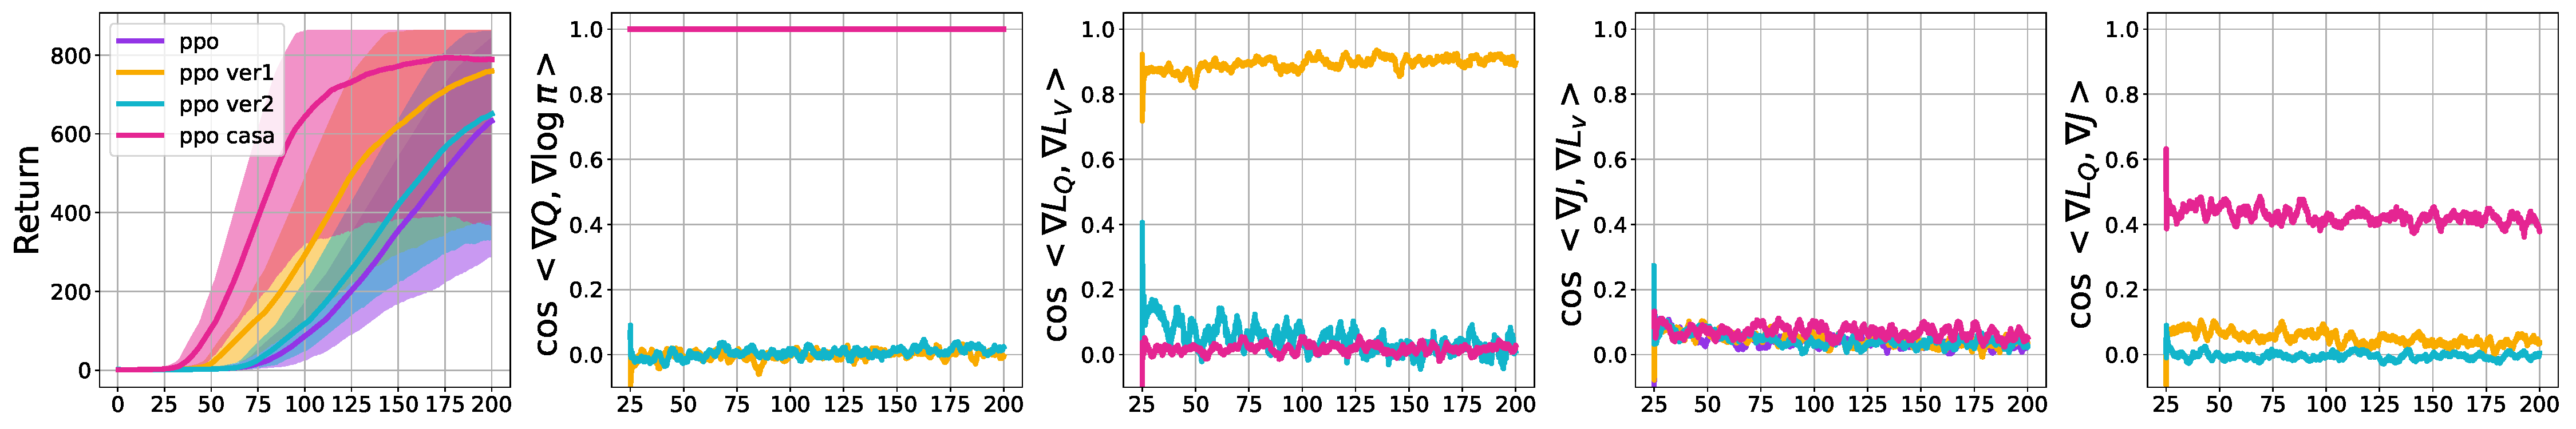
\includegraphics[width=\linewidth]{body/app_fig/app_ppo_Breakout.pdf}

% 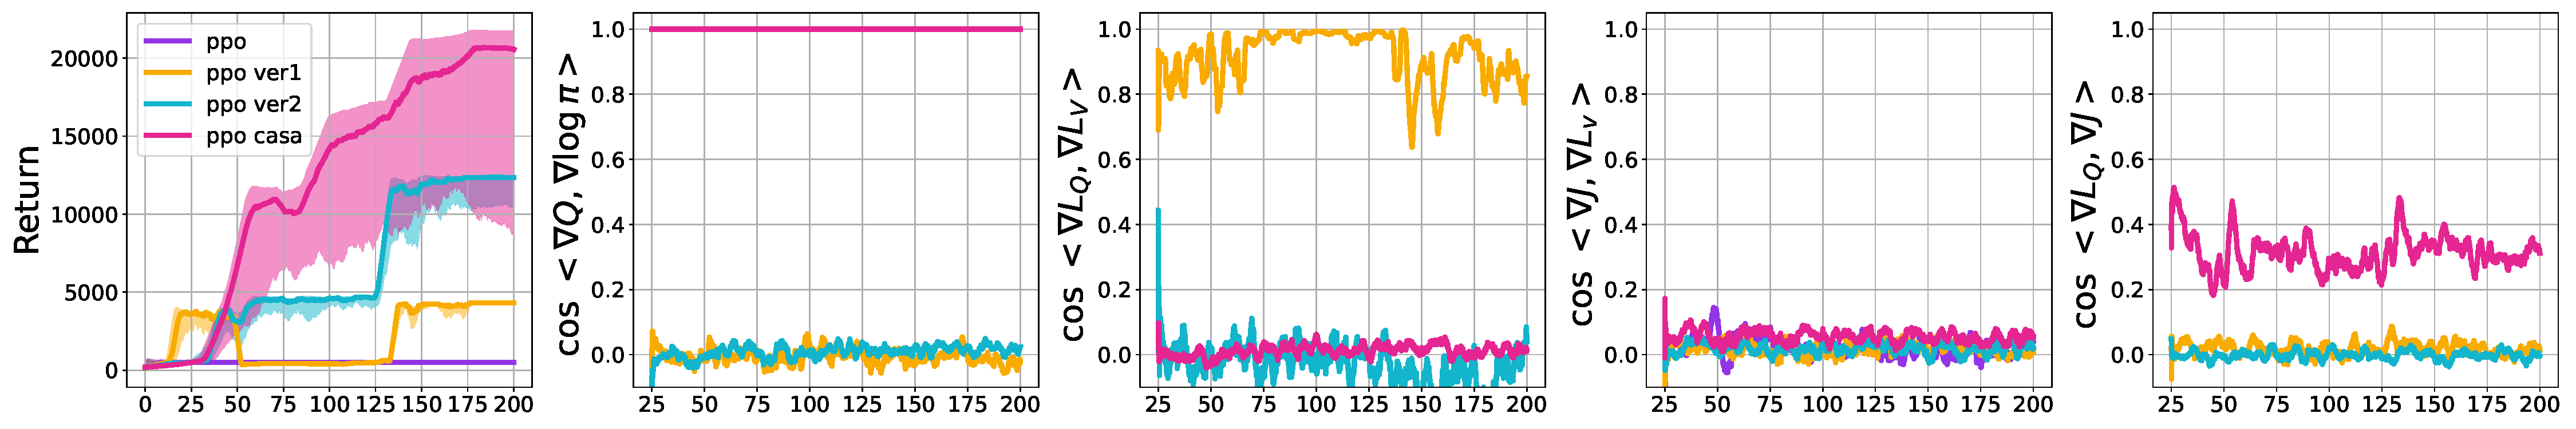
\includegraphics[width=\linewidth]{body/app_fig/app_ppo_Qbert.pdf}

% 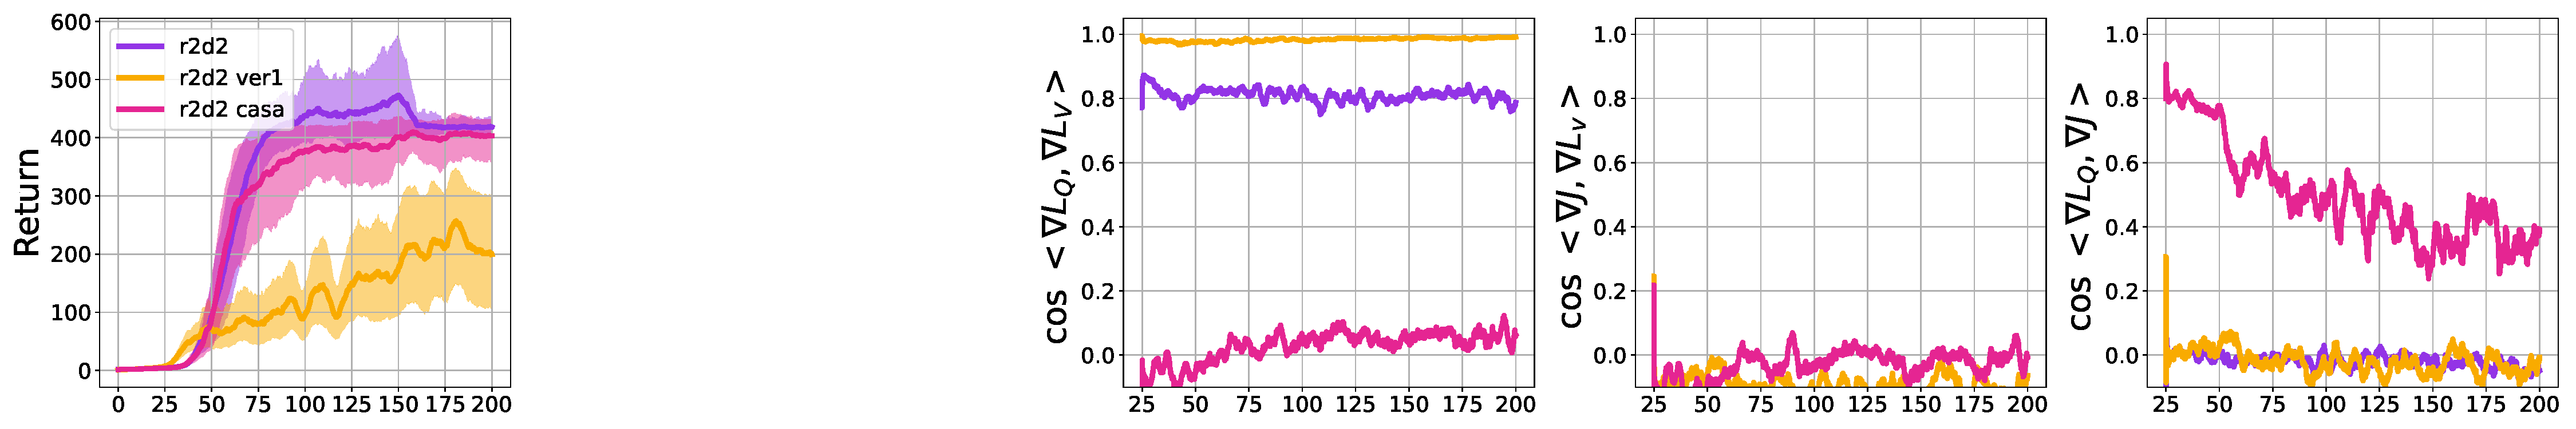
\includegraphics[width=\linewidth]{body/app_fig/app_r2d2_Breakout.pdf}


% 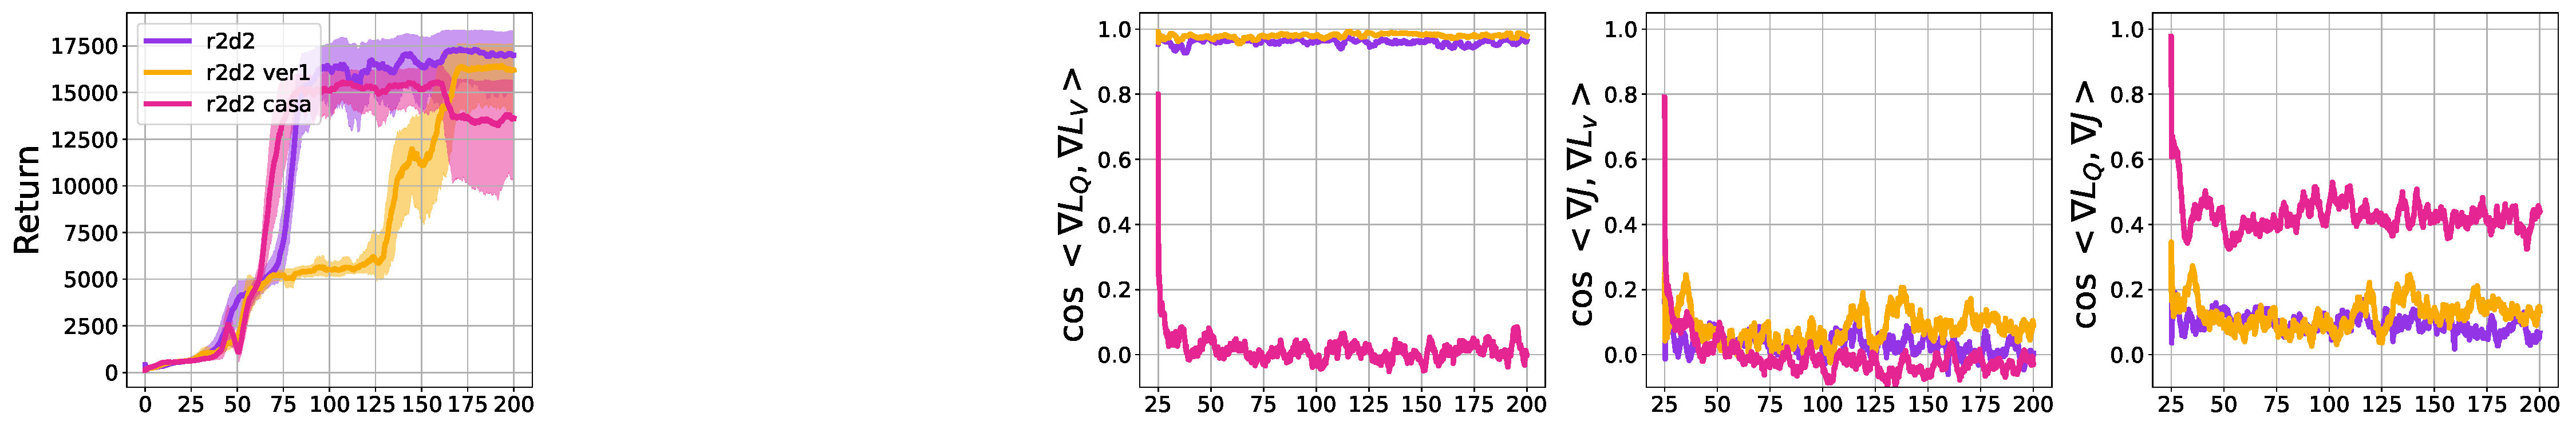
\includegraphics[width=\linewidth]{body/app_fig/app_r2d2_Qbert.pdf}
% \caption{Angles of Gradients and Returns of versions of PPO and R2D2 defined in Table \ref{tab:ppo_mtv} and Table \ref{tab:r2d2_mtv}.}
% \label{fig:mtv_app}
% \end{figure}

% \clearpage

% \changnan{casa summary deleted}
% \section{CASA summary}
% \begin{figure}[ht]
% \centering
% 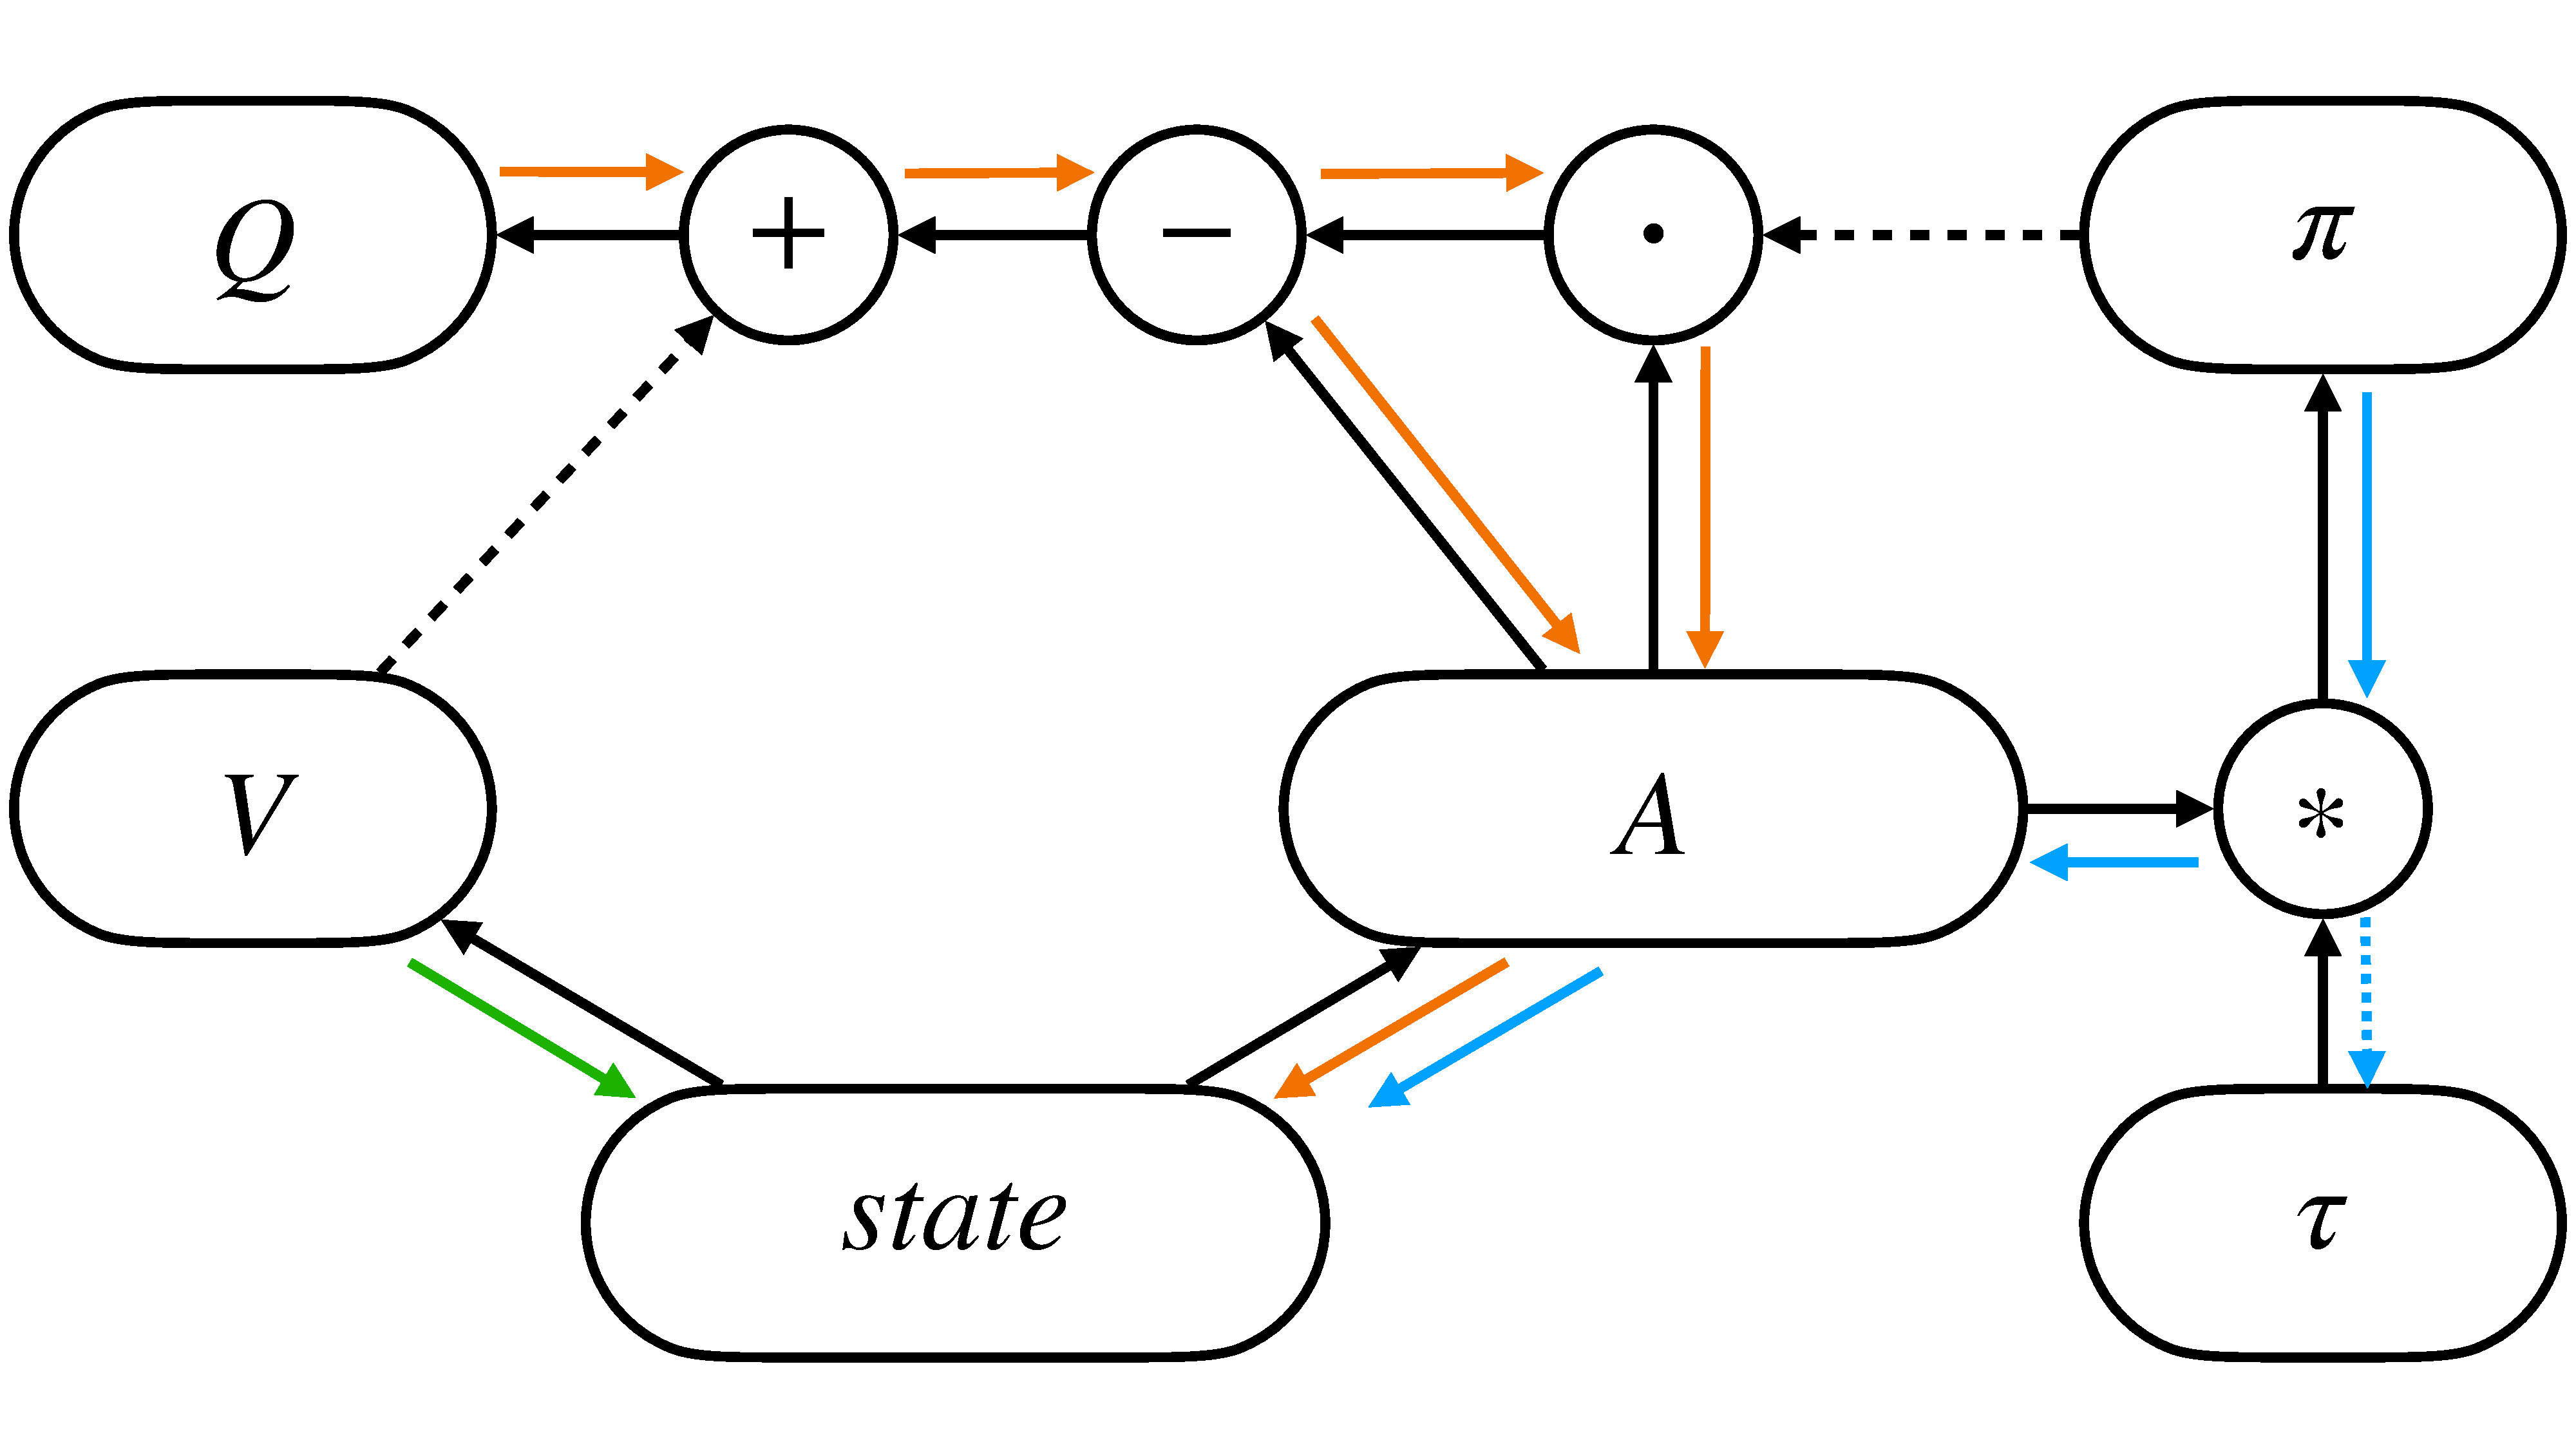
\includegraphics[width=0.4\textwidth,bb= 0 0 1800 1100]{body/figures/CASA.pdf}
% \caption{
% \textbf{Black} lines represent the forward process.
% \textbf{Dotted} black lines represent the \textit{stop gradient} operator in the forward process. 
% \textbf{Colorful} lines represent backpropagation from different loss functions. 
% Specifically, \textbf{blue} lines represent $\mathbb{E}_\pi [(Q^\pi-V)\nabla \log \pi]$, 
% \textbf{orange} lines represent $\mathbb{E}_\pi [(Q^\pi-Q)\nabla Q]$,
% and \textbf{green} lines represent $\mathbb{E}_\pi [(Q^\pi-V)\nabla V]$.}
% \label{fig:casa}
% \end{figure}
% \section{motivation experiments}

\clearpage

{\colorred \section{On Discussing Application of CASA on Continuous Action Space}
\label{app:cts_space}

As we can see CASA is only applied to discrete action space in the main context, we make a discussion on whether CASA is applicable on continuous action space. 
For brevity, we let $\tau=1$ and write \eqref{eq:casa} as:
\begin{equation}
\left\{
    \begin{aligned}
        &\pi = \text{softmax}(A), \\
        &\Bar{A} = A - \mathbb{E}_{\pi} [A], \\
        &Q = \Bar{A} + sg(V).
    \end{aligned}
\right. 
\end{equation}
The difficulty comes from estimating two quantities, one is $\text{softmax}(A)$, the other is $\mathbb{E}_{\pi} [A]$. 
This comes from the fact that discrete action space is countable so these two quantities are expressed in a closed-form, while continuous action space is uncountable so an accurate estimation of these two quantities is intractable. 
We can surely apply Monte Carlo methods to approximate, but a more elegant close-form expression may be preferred. 
Then this becomes another problem: \textit{how to estimate (state-action values / advantages / policy probabilities) of all actions in a continuous action space efficiently without loss of generality?}
This is another representational design problem, which is out of scope of this paper, so we don't touch much about it. 
But with the hope of inspiring a better solution to this problem, we provide one practical way of applying CASA on continuous action space based on kernel-based machine learning. 

Let $a_0, \dots, a_k$ to be basis actions in the action space. 
Let $A(s, a_0), \dots, A(s, a_k)$ to be advantage functions for tuples of states and basis actions. 
They can either share parameters or be isolated. 
Let $K(\cdot, \cdot)$ be a kernel function defined on the product of two action spaces. 
For any $a$ in the action space, we can estimate $A(s, a)$ by a decomposition such like $$A(s, a) = \frac{1}{Z_a} (K(a_0, a) A(s, a_0) + \dots + K(a_k, a) A(s, a_k)),$$ where $Z_a = \sum_{i=0}^k K(a_i, a)$ is a normalization constant. 

Since $K(\cdot, a)$ is a closed-form function of $a$, and $|\{A(s, a_0), \dots, A(s, a_k)\}|$ is finite, we can make a closed-form expression of both $\text{softmax}(A)$ and $\mathbb{E}_{\pi} [A]$. 
Then we can apply CASA directly on this expression, with one function estimates $V$ and the other function estimates advantages of all actions in a closed-form with only state as input.  
The policy is defined directly by $\text{softmax}$ of all advantages. 
In details, we define
\begin{equation}
\left\{
    \begin{aligned}
        &\pi(s, a) = \exp (A(s, a)) / \int_{a} \exp (A(s, a)) da, \\
        &\Bar{A}(s, a) = A(s, a) - \int_{a} sg(\pi(s, a)) A(s, a) da, \\
        &Q(s, a) = \Bar{A}(s, a) + sg(V(s)).
    \end{aligned}
\right. 
\end{equation}

Then it satisfies the consistency of CASA on continuous action space.
$$
\begin{aligned}
    \nabla \log \pi(s, a) &= \nabla A(s, a) - \frac{\nabla \int_{a} \exp (A(s, a)) da}{\int_{a} \exp (A(s, a)) da} \\
    &= \nabla A(s, a) - \frac{ \int_{a} \exp (A(s, a)) \nabla A(s, a) da}{\int_{a} \exp (A(s, a)) da} \\
    &= \nabla A(s, a) - \int_{a} \frac{  \exp (A(s, a)) }{\int_{a} \exp (A(s, a)) da} \nabla A(s, a) da \\
    &= \nabla A(s, a) - \int_{a} \pi(s, a) \nabla A(s, a) da \\
    &= \nabla \Bar{A}(s, a) = \nabla Q(s, a). 
\end{aligned}
$$
}

\section{DR-Trace}
\label{app:drtrace}

% One simple choice is to learn $V$ and $\pi$ by V-Trace \citep{impala} and to learn $Q$ by ReTrace \citep{retrace}. 
% \citep{impala} shows that $V^{\Tilde{\pi}}$ estimated by V-Trace converges to $V^*$ that corresponds to some $\Tilde{\pi}_{VTrace}$.
% Respectively, \citep{retrace} shows that $Q^{\Tilde{\pi}}$ estimated by ReTrace converges to $Q^*$ that corresponds to some $\Tilde{\pi}_{ReTrace}$.

As CASA estimates $(V, Q, \pi)$, we would ask
\textbf{i)} how to guarantee that $\Tilde{\pi}_{VTrace} = \Tilde{\pi}_{ReTrace}$, 
\textbf{ii)} how to exploit $(V, Q, \pi)$ to make a better estimation. 
Though we can apply V-Trace to estimate $V$ and ReTrace to estimate $Q$ with proper hyperparameters to guarantee $\Tilde{\pi}_{VTrace} = \Tilde{\pi}_{ReTrace}$, it's more reasonable to estimate $(V, Q)$ together. 
Inspired by Doubly Robust, which is shown to maximally reduce the variance, we introduce DR-Trace, which estimates $V$ by 
$$
\label{eq:dr-v}
    \begin{aligned}
        V_{DR}^{\Tilde{\pi}} (s_t) &\overset{def}{=} \mathbb{E}_{\mu} [ 
        V(s_t) + \sum_{k \geq 0} \gamma^k 
     c_{[t:t+k-1]} \rho_{t+k}  \delta^{DR}_{t+k} ],  
    \end{aligned}
$$
{\colorred where $\mu$ is the behavior policy}, $\delta^{DR}_t \overset{def}{=} r_t + \gamma V(s_{t+1}) - Q(s_t, a_t)$ is one-step Doubly Robust error, $\rho_t \overset{def}{=} \min\{\frac{\pi_t}{\mu_t}, \Bar{\rho} \}$ and $c_t \overset{def}{=} \min\{\frac{\pi_t}{\mu_t}, \Bar{c}\}$ are clipped per-step importance sampling, $c_{[t: t+k]} \overset{def}{=} \prod_{i=0}^{k} c_{t+i}$.

With one step Bellman equation, we estimate $Q$ by
$$
\label{eq:dr-q}
    \begin{aligned}
         Q_{DR}^{\Tilde{\pi}} (s_t, a_t) 
         &\overset{def}{=} \mathbb{E}_{s_{t+1}, r_t \sim p(\cdot, \cdot | s_t, a_t)} [  r_t + \gamma   V_{DR}^{\Tilde{\pi}} (s_{t+1}) ] 
        \\
        %  &=  \mathbb{E}_{\mu} [ r_t + \gamma V(s_{t + 1}) +
        % \gamma \sum_{k \geq 0} \gamma^k 
        % c_{[t+1:t+k]} \rho_{t+1+k}
        % \delta^{DR}_{t+1+k} V
        % ]
        % \\
        %  &= \mathbb{E}_{\mu}   [
        % Q(s_t, a_t) + \delta_t^{DR}V + \sum_{k \geq 1}  \gamma^k
        % c_{[t+1:t+k-1]} \rho_{t+k}
        % \delta^{DR}_{t+k} V
        % ],
        % \\
        &=  \mathbb{E}_{\mu}   [
        Q(s_t, a_t) + \sum_{k \geq 0}  \gamma^k
        c_{[t+1:t+k-1]} \Tilde{\rho}_{t, k}
        \delta^{DR}_{t+k}
        ], 
    \end{aligned}
$$
where $\Tilde{\rho}_{t, k} =  1_{\{k=0\}} + 1_{\{k > 0\}} \rho_{t+k}$.

% Compared to \eqref{eq:dr-v}, $c_{[t+1:t+k-1]} \Tilde{\rho}_{t, k}$ in \eqref{eq:dr-q} doesn't multiply importance sampling ratio of $a_t$, which meets the same intuition as \eqref{eq:vtrace} and \eqref{eq:retrace}.\\
\begin{theorem}
    Define $\Bar{A} = A - \mathbb{E}_\pi[A]$, $Q = \Bar{A} + sg(V)$,
    $$
    \begin{aligned}
    &\mathscr{T}(Q) \overset{def}{=} \mathbb{E}_{\mu}   [
        Q(s_t, a_t) + \sum_{k \geq 0}  \gamma^k
        c_{[t+1:t+k-1]} \Tilde{\rho}_{t, k}
        \delta^{DR}_{t+k}
        ], \\
    &\mathscr{S}(V) \overset{def}{=} \mathbb{E}_{\mu}   [
        V(s_t) + \sum_{k \geq 0}  \gamma^k
        c_{[t:t+k-1]} \rho_{t, k}
        \delta^{DR}_{t+k}
        ], \\
    &\mathscr{U}(Q, V) = (\mathscr{T}(Q) - \mathbb{E}_\pi[Q] + \mathscr{S}(V), \mathscr{S}(V)), \\
    &\mathscr{U}^{(n)}(Q, V) = \mathscr{U}(\mathscr{U}^{(n-1)}(Q, V)),
    \end{aligned}
    $$
    then $\mathscr{U}^{(n)}(Q, V) \rightarrow (Q^{\Tilde{\pi}}, V^{\Tilde{\pi}})$ that corresponds to 
    $$
        \Tilde{\pi}(a|s) = \frac
        {\min \left\{\Bar{\rho} \mu (a|s), \pi(a|s)\right\}}
        {\sum_{b \in \mathcal{A}}\min \left\{\Bar{\rho} \mu (b|s), \pi(b|s)\right\}}.
    $$ as $n \rightarrow +\infty$.
\label{thm:dr}
\end{theorem}
\begin{proof}
    See Appendix \ref{app:proof}, Theorem \ref{thm_app:dr}.
\end{proof}
Theorem \ref{thm:dr} shows that DR-Trace is a contraction mapping and $(V, Q)$ converges to $(V^{\Tilde{\pi}}, Q^{\Tilde{\pi}})$ that corresponds to 
$$
    \begin{aligned}
        \Tilde{\pi}(a|s) = \frac
        {\min \left\{\Bar{\rho} \mu (a|s), \pi(a|s)\right\}}
        {\sum_{b \in \mathcal{A}}\min \left\{\Bar{\rho} \mu (b|s), \pi(b|s)\right\}}.
    \end{aligned}
$$

% At training time, the policy evaluation is achieved by updating $\theta$ to minimize $l2$ losses
% $$
% \begin{aligned}
%     L_V(\theta) &= \mathbb{E}_\pi [ (V_\theta(s_t) -  V_{DR}^{\Tilde{\pi}} (s_t))^2 ], \\
%     L_Q(\theta) &= \mathbb{E}_\pi [ (Q_\theta(s_t, a_t) -  Q_{DR}^{\Tilde{\pi}} (s_t, a_t))^2 ],
% \end{aligned}
% $$ 
% which gives the ascent direction of $\theta$ by
% \begin{equation}
% \label{eq:grad_qv}
%     \begin{aligned}
%         \nabla_\theta L_V(\theta)
%         &= \mathbb{E}_\pi \left[ (V_{DR}^{\Tilde{\pi}} (s_t) - V_\theta(s_t) ) \nabla V_\theta(s_t) \right], \\
%         \nabla_\theta L_Q(\theta)
%         &= \mathbb{E}_\pi \left[ (Q_{DR}^{\Tilde{\pi}} (s_t, a_t) - Q_\theta(s_t, a_t)) \nabla Q_\theta(s_t, a_t) \right].
%     \end{aligned}
% \end{equation}
% And we make the policy improvement by policy gradient, which gives the ascent direction of $\theta$ by 
% \begin{equation}
% \label{eq:grad_pi}
% \begin{aligned}
%     \nabla_\theta \mathcal{J}(\tau, \theta) = \mathbb{E}_\mu \left[\tau \rho_t (Q_{DR}^{\Tilde{\pi}} (s_t, a_t) - V_\theta(s_t) ) \nabla_\theta \log \pi_t \right],
% \end{aligned}
% \end{equation}
% where $\mathcal{J} (\tau, \theta) = \tau \mathbb{E}_\pi [\sum \gamma^t r_t]$.
% It takes an additional $\tau$, which frees the scale of gradient from $\tau$.

% Finally, the gradient ascent direction of $\theta$ is given by
% \begin{equation}
%     \label{eq:grad_all}
%     \alpha_1 \nabla_\theta L_V + \alpha_2 \nabla_\theta L_Q + \alpha_3 \nabla_\theta \mathcal{J}.
% \end{equation}

% \textbf{Full algorithm is described in Appendix \ref{app:casa}.}
% Note that \eqref{eq:grad_all} doesn't need any entropy regularization. 
% We will discuss why this happens in section \ref{sec:equiv} and how CASA controls the exploration in section \ref{sec:ent_control}.


\begin{figure}[h]
    \centering
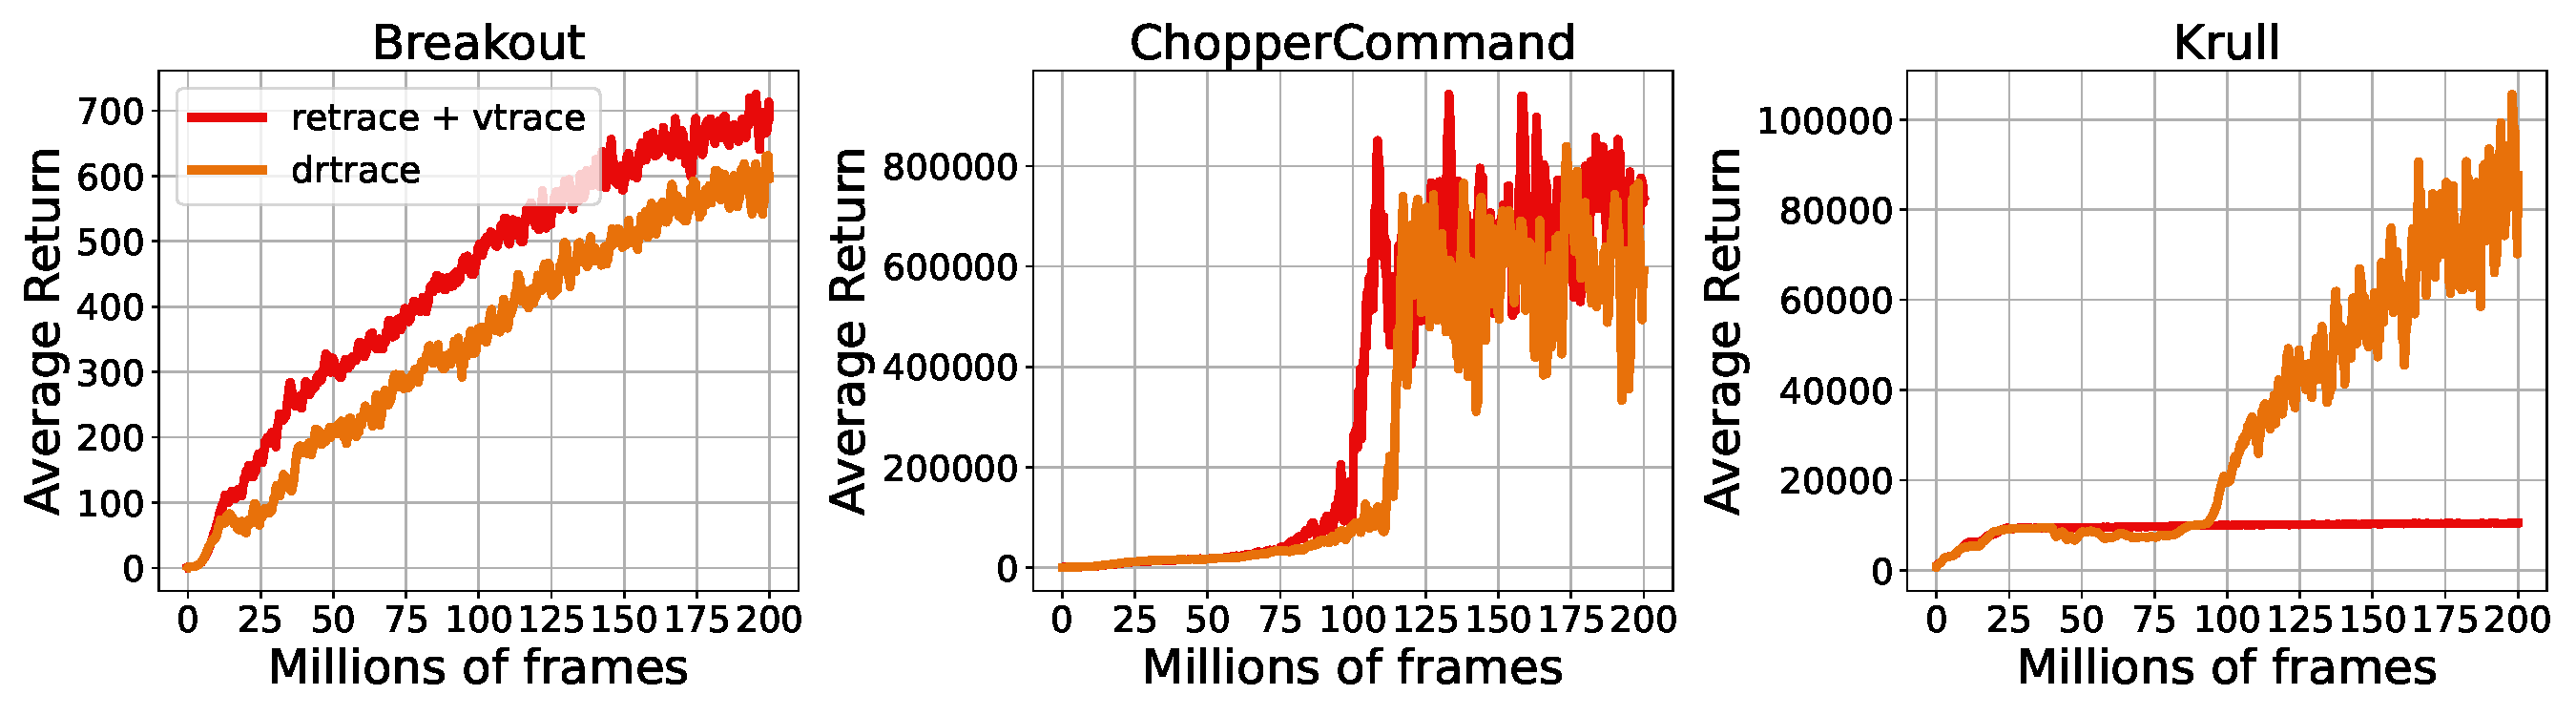
\includegraphics[width=\linewidth]{body/ablation/dr_ablation.pdf}
    \caption{Ablation study for w/wo DR-Trace on Breakout, ChopperCommand and Krull.}
    \label{fig:app_dr_trace}
\end{figure}

According to our proof, DR-Trace should work similar to V-Trace and ReTrace, as the convergence rate and the limitation are same. 
We compare DR-Trace with V-Trace+ReTrace in Figure \ref{fig:app_dr_trace}, where we replace estimation of state values by V-Trace and estimation of state-action values by ReTrace. 
We call V-Trace+ReTrace as No-DR-Trace for brevity. 
No-DR-Trace performs better on Breakout and ChopperCommand, but fails to make a breakthrough on Krull. 
Recalling the fact that Doubly Robust can maximally reduce the variance of Bellman error, No-DR-Trace is less stable but also potential to achieve a better performance. 
A conclusion cannot be made about No-DR-Trace, as this phenomenon means that No-DR-Trace is less stable than DR-Trace, but it also holds the potential to achieve a better performance.

% \clearpage


\section{Proofs}
\label{app:proof}

\theoremstyle{plain}
% \setcounter{Lemma}{0}
\newtheorem{Lemma_app}{Lemma}[section]
\newtheorem{Theorem_app}{Theorem}[section]
\theoremstyle{definition}
\newtheorem*{Remark_app}{Remark}
\theoremstyle{remark}

% \begin{Lemma_app}
% Let 
% $g \in \textbf{C}^{1}(\mathbb{R}^{n}): \mathbb{R}^{n} \to \mathbb{R}^{n}, \ f \in \textbf{C}^{1}(\mathbb{R}^{n+k}): \mathbb{R}^{n+k} \to \mathbb{R}^{n}.
% $\\
% If
% $
% \nabla_x g(x) = \nabla_x f(x, y)$, for $\forall x\in \mathbb{R}^{n}, y\in \mathbb{R}^k,
% $
% then $\exists$ $c \in \textbf{C}^{1}(\mathbb{R}^{k}): \mathbb{R}^{k} \to \mathbb{R}^{n}$, s.t. $f(x, y) = g(x) + c(y)$.
% \label{lemma_app:func_sep}
% \end{Lemma_app}
% \begin{proof}

% Let $\Tilde{f}(x, y) = f(x, y) - g(x)$.

% Since $\nabla_x g(x) = \nabla_x f(x, y)$, we have 
% $$
% \nabla_x \Tilde{f} = 0, \ for \ \forall x\in \mathbb{R}^{n}, y\in \mathbb{R}^k.
% $$

% So $\Tilde{f}$ is a constant function w.r.t $x$, which can be denoted as $c(y) = \Tilde{f}(x, y)$.

% Hence, $f(x, y) = g(x) + c(y)$.
% \end{proof}

\begin{Lemma_app}
(i) Define $\pi = softmax(A / \tau)$, then $\nabla \log \pi = (\textbf{1} - \pi) \frac{\nabla A}{\tau}$. 
(ii) Denote $sg$ to be stop gradient and define $\Bar{A} = A - \mathbb{E}_\pi [A]$, $Q = \Bar{A} + sg(V)$, then $\nabla Q = (\textbf{1} - \pi) \nabla A$.
\label{lemma_app:vannila_grad}
\end{Lemma_app}
\begin{proof}

As $Q = \Bar{A} + sg(V) = A - sg(\pi)\cdot A + sg(V)$, it's obvious that $\nabla Q = (\textbf{1} - \pi) \nabla A$.

For $\log \pi$, it's a standard derivative of cross entropy, so we have $\nabla \log \pi = (\textbf{1} - \pi) \nabla (A / \tau) = (\textbf{1} - \pi) \frac{\nabla A}{\tau}$.
\end{proof}

\begin{Lemma_app}
Define $\Bar{A}= A - \mathbb{E}_\pi[A]$, $Q = \Bar{A} + sg(V), \pi = softmax(A / \tau)$, then 
$$
\mathbb{E}_\pi \left[ (Q - V) \nabla \log \pi \right]
= - \tau \nabla \textbf{H}[\pi].
$$
\label{lemma_app:eqiv_pg_ent}
\end{Lemma_app}
\begin{proof}
Since 
$$
\pi = \exp(A / \tau) / Z,\ Z = \int_\mathcal{A} \exp(A / \tau),
$$
we have 
$$
A = \tau \log \pi + \tau \log Z.
$$
Based on the observation that $\mathbb{E}_\pi \left[ f(s) \nabla \log \pi (\cdot | s) \right] = 0$, 
we have 
$$\mathbb{E}_\pi \left[ \mathbb{E}_\pi[A] \cdot \nabla \log \pi \right] = 0,$$ 
$$\mathbb{E}_\pi \left[ \log Z \cdot \nabla \log \pi \right] = 0.$$

On the one hand,
$$
\begin{aligned}
    \mathbb{E}_\pi \left[ (Q - V) \nabla \log \pi \right]
    &= \mathbb{E}_\pi \left[ A \nabla \log \pi \right] 
    - \mathbb{E}_\pi \left[ \mathbb{E}_\pi[A] \cdot \nabla \log \pi \right] \\
    &= \tau \mathbb{E}_\pi \left[ \log \pi \nabla \log \pi \right]
    + \tau \mathbb{E}_\pi \left[ \log Z \cdot \nabla \log \pi \right] \\
    &= \tau \mathbb{E}_\pi \left[ \log \pi \nabla \log \pi \right].
\end{aligned}
$$

On the other hand, 
$$
\begin{aligned}
    \nabla \textbf{H} [\pi] 
    &= - \nabla \int_\mathcal{A} \pi_i \log \pi_i \\
    &= - \int_\mathcal{A}  \nabla \pi_i \cdot \log \pi_i - \int_\mathcal{A} \pi_i \nabla \log \pi_i  \\
    &= - \int_\mathcal{A}  \pi_i \nabla \log \pi_i \cdot \log \pi_i - \int_\mathcal{A}  \pi_i \frac{\nabla \pi_i}{\pi_i} \\
    &= - \mathbb{E}_\pi \left[ \log \pi \nabla \log \pi \right].
\end{aligned}
$$
Hence, $
\mathbb{E}_\pi \left[ (Q - V) \nabla \log \pi \right]
= - \tau \nabla \textbf{H}[\pi]
$.
\end{proof}

\begin{Theorem_app}
    Define $\Bar{A} = A - \mathbb{E}_\pi[A]$, $Q = \Bar{A} + sg(V)$.
    Define $$
    \begin{aligned}
    &\mathscr{T}(Q) \overset{def}{=} \mathbb{E}_{\mu}   [
        Q(s_t, a_t) + \sum_{k \geq 0}  \gamma^k
        c_{[t+1:t+k-1]} \Tilde{\rho}_{t, k}
        \delta^{DR}_{t+k}
        ], \\
    &\mathscr{S}(V) \overset{def}{=} \mathbb{E}_{\mu}   [
        V(s_t) + \sum_{k \geq 0}  \gamma^k
        c_{[t:t+k-1]} \rho_{t, k}
        \delta^{DR}_{t+k}
        ], \\
    &\mathscr{U}(Q, V) = (\mathscr{T}(Q) - \mathbb{E}_\pi[Q] + \mathscr{S}(V), \mathscr{S}(V)), \\
    &\mathscr{U}^{(n)}(Q, V) = \mathscr{U}(\mathscr{U}^{(n-1)}(Q, V)),
    \end{aligned}
    $$
    then $\mathscr{U}^{(n)}(Q, V) \rightarrow (Q^{\Tilde{\pi}}, V^{\Tilde{\pi}})$ that corresponds to 
    $$
        \Tilde{\pi}(a|s) = \frac
        {\min \left\{\Bar{\rho} \mu (a|s), \pi(a|s)\right\}}
        {\sum_{b \in \mathcal{A}}\min \left\{\Bar{\rho} \mu (b|s), \pi(b|s)\right\}}.
    $$ as $n \rightarrow +\infty$.
\label{thm_app:dr}
\end{Theorem_app}
\begin{Remark_app}
$\mathscr{T}(Q) - \mathbb{E}_\pi[Q] + \mathscr{S}(V)$ is \textbf{exactly} how $Q$ is updated at training time. 
Since $Q = \Bar{A} + sg(V)$, if we apply gradient ascent on $Q$ and $V$ in directions $\nabla L_Q(\theta)$ and $\nabla L_V(\theta)$ respectively, change of $Q$ comes from two aspects. One comes from $\nabla L_Q(\theta)$, which changes $A$, the other comes from $\nabla L_V(\theta)$, which changes $V$. Because the gradient of $V$ is stopped when estimating $Q$, the latter is captured by "minus old baseline, add new baseline", which is $- \mathbb{E}_\pi[Q] + \mathscr{S}(V)$ in Theorem \ref{thm_app:dr}.
\end{Remark_app}
\begin{proof}
 Define
 $$
 \begin{aligned}
        \widetilde{\mathscr{T}}(Q) &= - \mathbb{E}_\pi[Q] + \mathscr{T}(Q), \\
        \widetilde{\mathscr{U}}(Q, V) &= (\widetilde{\mathscr{T}}(Q), \mathscr{S}(V)), \\
        \widetilde{\mathscr{U}}^{(n)}(Q, V) &=   \widetilde{\mathscr{U}}(\widetilde{\mathscr{U}}^{(n-1)}(Q, V)).
 \end{aligned}
 $$
By Lemma \ref{lemma_app:dr_q}, $\widetilde{\mathscr{T}}^{(n)}(Q)$ converges to some $A^*$ as $n \rightarrow \infty$. This process will not influence the estimation of $V$ as the gradient of $V$ is stopped when estimating $Q$. According to the proof, $A^*$ does not depend on $V$. \\
By Lemma \ref{lemma_app:dr_v}, $\mathscr{S}^{(n)}(V)$ converges to some $V^*$ as $n \rightarrow \infty$. \\
Hence, we have
$$
\widetilde{\mathscr{U}}^{(n)}(Q, V) \rightarrow (A^*, V^*)\ \ as\ \ n \rightarrow +\infty. 
$$
By definition, 
$$
\mathscr{U}(Q, V) = (\widetilde{\mathscr{T}}(Q) + \mathscr{S}(V), \mathscr{S}(V)),
$$
we can regard $\widetilde{\mathscr{T}}(Q) + \mathscr{S}(V)$ as $Q$ and regard $\mathscr{S}(V)$ as $V$, then
$$
\begin{aligned}
    \mathscr{U}^{(2)}(Q, V) 
    &= \mathscr{U}(\widetilde{\mathscr{T}}(Q) + \mathscr{S}(V), \mathscr{S}(V)) \\
    &= (\mathscr{T}(\widetilde{\mathscr{T}}(Q) + \mathscr{S}(V)) -\mathscr{S}(V) + \mathscr{S}^{(2)}(V), \mathscr{S}^{(2)}(V)) \\
    &= (\widetilde{\mathscr{T}}^{(2)}(Q) + \mathscr{S}^{(2)}(V), \mathscr{S}^{(2)}(V)).
\end{aligned}
$$
By induction, 
$$
\begin{aligned}
    \mathscr{U}^{(n)}(Q, V) &= (\widetilde{\mathscr{T}}^{(n)}(Q) + \mathscr{S}^{(n)}(V), \mathscr{S}^{(n)}(V)) \\
    &\rightarrow (A^*+V^*, V^*)\ \ as\ \ n\rightarrow + \infty.
\end{aligned}
$$
Same as \citep{impala}, 
$$
    \Tilde{\pi}(a|s) = \frac
    {\min \left\{\Bar{\rho} \mu (a|s), \pi(a|s)\right\}}
    {\sum_{b \in \mathcal{A}}\min \left\{\Bar{\rho} \mu (b|s), \pi(b|s)\right\}}.
$$ 
is the policy s.t. the Bellman equation holds, which is 
$$\mathbb{E}_\mu[\rho_t (r_t + \gamma V_{t+1} - V_t) | \mathscr{F}_t] = 0,$$ and $\mathscr{U}(Q^{\Tilde{\pi}}, V^{\Tilde{\pi}}) = (Q^{\Tilde{\pi}}, V^{\Tilde{\pi}})$. \\
So we have
$(A^*+V^*, V^*) = (Q^{\Tilde{\pi}}, V^{\Tilde{\pi}}).$
\end{proof}

\begin{Lemma_app}
Define $\Bar{A}= A - \mathbb{E}_\pi[A]$, $Q = \Bar{A} + sg(V)$,
then operator 
$$
    \mathscr{T}(Q) \overset{def}{=} \mathbb{E}_{\mu}   [
        Q(s_t, a_t) + \sum_{k \geq 0}  \gamma^k
        c_{[t+1:t+k-1]} \Tilde{\rho}_{t, k}
        \delta^{DR}_{t+k}
        ]
$$
is a contraction mapping w.r.t. $Q$.
\label{lemma_app:dr_q}
\end{Lemma_app}
\begin{Remark_app}
Note that $\mathscr{T}(Q)$ is exactly \eqref{eq:dr-q}. 

Since $Q = A + sg(V)$, the gradient of $V$ is stopped when estimating $Q$, updating $Q$ will not change $V$, which is equivalent to updating $A$.
Without loss of generality, we assume $V$ is fixed as $V^*$ in the proof.
\end{Remark_app}
\begin{proof}

$\Bar{A} = A - \mathbb{E}_\pi[A]$ shows $\mathbb{E}_\pi[\Bar{A}] = 0$, which guarantees that no matter how we update $A$, we always have $\mathbb{E}_\pi[Q] = V^*$.

Based on above observations, define 
$$
    \widetilde{\mathscr{T}}(Q) \overset{def}{=} - \mathbb{E}_\pi [Q] + \mathscr{T}(Q).
$$

It's obvious that we only need to prove $\widetilde{\mathscr{T}}(Q)$ is a contraction mapping.

For brevity, we denote $$Q_t = Q(s_t, a_t), A_t = A(s_t, a_t), V^*_t = V^*(s_t).$$

Noticing that $\Tilde{\rho}_{t, 0} = 1$, let $\mathscr{F}$ represent filtration, we can rewrite $\widetilde{\mathscr{T}}$ as 
\begin{equation}
\label{eq:dr_a_2}
\begin{aligned}
    \widetilde{\mathscr{T}}(Q)
    &= \mathbb{E}_{\mu}   [
        A_t + \sum_{k \geq 0}  \gamma^k
        c_{[t+1:t+k-1]} \Tilde{\rho}_{t, k}
        \delta^{DR}_{t+k}
        ] \\
    &= \mathbb{E}_{\mu}   [
        -V^*_t + \sum_{k \geq 0}  \gamma^k
        c_{[t+1:t+k-1]} \Tilde{\rho}_{t, k}
        r_{t+k}
        + 
        \sum_{k \geq 0}  \gamma^{k+1}
        c_{[t+1:t+k-1]} \Delta_k ],
        \\
\end{aligned}
\end{equation}
where 
\begin{equation}
\label{eq:dr_delta}
    \Delta_k = \mathbb{E}_{\mu}\left[\Tilde{\rho}_{t, k} V^*_{t+k+1} - c_{t+k} \Tilde{\rho}_{t, k+1} Q_{t+k+1} | \mathscr{F}_{t+k}\right].
\end{equation}
By definition of $Q$,
$$
    \mathbb{E}_{\mu}[V_{t+k+1}^*|\mathscr{F}_{t+k}] 
    = \mathbb{E}_{\mu}[
    \mathbb{E}_\pi[Q_{t+k+1}|\mathscr{F}_{t+k+1}]
    |\mathscr{F}_{t+k}], \\
    % \geq&  \mathbb{E}_{\mu}[
    % \mathbb{E}_\mu[\Tilde{\rho}_{t, k+1} Q_{t+k+1}|\mathscr{F}_{t+k+1}]
    % |\mathscr{F}_{t+k}], 
$$
we can rewrite \eqref{eq:dr_delta} as
\begin{equation}
\label{eq:dr_q_delta}
\Delta_k = \mathbb{E}_{\mu}[
(
\Tilde{\rho}_{t, k} \frac{\pi_{t+k+1}}{\mu_{t+k+1}}- c_{t+k} \Tilde{\rho}_{t, k+1} 
) Q_{t+k+1} | \mathscr{F}_{t+k}
].
\end{equation}
For any $Q_1 = A_1 + sg(V^*)$, $Q_2 = A_2 + sg(V^*)$, since
$$
\mathbb{E}_{\mu}[
(
\Tilde{\rho}_{t, k} \frac{\pi_{t+k+1}}{\mu_{t+k+1}}- c_{t+k} \Tilde{\rho}_{t, k+1} 
) | \mathscr{F}_{t+k}
] \geq 0,
$$
by \eqref{eq:dr_a_2} \eqref{eq:dr_q_delta}, we have 
% $$
% || \Delta^1_k - \Delta_k^2 || \leq \mathbb{E}_{\mu}\left[
% \left(
% \Tilde{\rho}_{t, k} \frac{\pi_{t+k+1}}{\mu_{t+k+1}}- c_{t+k} \Tilde{\rho}_{t, k+1} 
% \right) | \mathscr{F}_{t+k}
% \right] ||A^1 - A_2||.
% $$
$$
        || \widetilde{\mathscr{T}}(Q_1) - \widetilde{\mathscr{T}}(Q_2) || 
        % \leq& \mathbb{E}_{\mu} \left[ \sum_{k \geq 0}  \gamma^{k+1} c_{[t+1:t+k-1]} || \Delta_k^1 - \Delta_k^2 || \right] \\
        \leq \mathcal{C} || Q_1 - Q_2 ||,
$$
where 
$$
    \begin{aligned}
        \mathcal{C} 
        &= \mathbb{E}_{\mu} [ \sum_{k \geq 0}  \gamma^{k+1} c_{[t+1:t+k-1]} 
        (
        \Tilde{\rho}_{t, k} \frac{\pi_{t+k+1}}{\mu_{t+k+1}}- c_{t+k} \Tilde{\rho}_{t, k+1} 
        ) ]
        \\
        &= \mathbb{E}_{\mu} [1 -1 + \sum_{k \geq 0}  \gamma^{k+1} c_{[t+1:t+k-1]} 
        \left(
        \Tilde{\rho}_{t, k} - c_{t+k} \Tilde{\rho}_{t, k+1} 
        \right) ] 
        \\
        &= 1 - (1 - \gamma)  \mathbb{E}_{\mu} [\sum_{k \geq 0} \gamma^{k}c_{[t+1:t+k-1]} \Tilde{\rho}_{t, k}  ] \\
        &\leq 1 - (1 - \gamma) < 1.
    \end{aligned}
$$
Hence, $\widetilde{\mathscr{T}}(Q)$ is a contraction mapping and converges to some fixed function, which we denote as $A^*$. So $\mathscr{T}(Q)$ is also a contraction mapping and converges to $A^*+V^*$.
\end{proof}

\begin{Lemma_app}
Define $Q = A + sg(V)$ with $\mathbb{E}_\pi [A] = 0$,
then operator 
$$
    \mathscr{S}(V) \overset{def}{=} \mathbb{E}_{\mu}  [
        V(s_t) + \sum_{k \geq 0}  \gamma^k
        c_{[t:t+k-1]} \rho_{t, k}
        \delta^{DR}_{t+k}
        ]
$$
is a contraction mapping w.r.t. $V$.
\label{lemma_app:dr_v}
\end{Lemma_app}
\begin{Remark_app}
Note that $\mathscr{S}(V)$ is exactly \eqref{eq:dr-v}. 
\end{Remark_app}
\begin{proof}

% Since $Q = A + sg(V)$, updating $V$ wouldn't influence $A$. WLOG, we assume $A$ is fixed as $A^*$ in Lemma \ref{lemma_app:dr_v}. \\
Same as Lemma \ref{lemma_app:dr_q}, we can get
$$
    \Delta_k = \mathbb{E}_{\mu}\left[
    \left( \rho_{t+k} - c_{t+k} \rho_{t+k+1}\right) V_{t+k+1} 
     -  c_{t+k} \rho_{t+k+1} A^*_{t+k+1} | \mathscr{F}_{t+k}\right],
$$
so we have 
$$
    \Delta^1_k - \Delta^2_k = \mathbb{E}_{\mu}\left[ 
    \left( \rho_{t+k} - c_{t+k} \rho_{t+k+1}\right) \cdot  
   (V^1_{t+k+1} -  V^2_{t+k+1})
     | \mathscr{F}_{t+k}\right].
$$
The remaining proof is identical to \citep{impala}'s.
\end{proof}

% \clearpage

% \begin{Lemma_app}
% Let $v \in \mathbb{R}^{|\mathcal{A}|}$ to be a vector. 
% Define 
% $
%     \pi (\tau) = \exp (v / \tau) / Z,\  Z = \int_\mathcal{A}  \exp(v / \tau).
% $
% Let $\Omega$ to be a probability measure supported on $[K, +\infty]$,
% then $f(\Omega) = \mathbb{E}_{\tau \sim \Omega} [\mathbb{E}_{\pi(\tau)} [v]]$ satisfies Lipschitz-1 condition with Wasserstein-1 metric.
% \label{lemma_app:lips}
% \end{Lemma_app}
% \begin{proof}
% Without loss of generality, we assume $v_1 \geq v_2 \geq ... \geq v_{|\mathcal{A}|}$.

% For any $\tau \in [0, +\infty)$, since
% $$
% \begin{aligned}
%     \pi (\tau) = \exp (v / \tau) / Z,\  Z = \int_\mathcal{A}  \exp(v / \tau),
% \end{aligned}
% $$
% we have
% $$
%     v = \tau \log \pi (\tau) + \tau \log Z.
% $$

% Denote $\Tilde{v}_j = v_j / \tau$. \\
% Since 
% $$
% \frac{\partial \log \pi_i}{\partial \Tilde{v}_j} = 1_{i=j} - \pi_j,
% $$
% we have
% $$
% \begin{aligned}
%     \frac{\partial \log \pi_i}{\partial \tau} 
%     &= \sum_j \frac{\partial \log \pi_i}{\partial \Tilde{v}_j} \cdot \frac{\partial \Tilde{v}_j}{\partial \tau} \\
%     &= - \sum_j (1_{i=j} - \pi_j) \frac{v_j}{\tau^2} \\
%     &= - \frac{1}{\tau^2} ( v_i - \sum_j \pi_j v_j ) \\ 
%     &= - \frac{1}{\tau^2} \left( v_i - \mathbb{E}_\pi [v] \right). 
% \end{aligned}
% $$
% Therefore, we have
% $$
% \begin{aligned}
%     \frac{\partial \pi_i}{\partial \tau} 
%     &= \pi_i \frac{\partial \log \pi_i}{\partial \tau} \\
%     &= - \frac{\pi_i}{\tau^2} \left( v_i - \mathbb{E}_\pi [v] \right).
% \end{aligned}
% $$
% Let $f(\tau) = v \cdot \pi(\tau)$, then
% $$
% \frac{\partial f}{\partial \tau} = - \frac{1}{\tau^2} \sum_i v_i \pi_i \left( v_i - \mathbb{E}_\pi [v] \right).
% $$
% Since $\sum_i \mathbb{E}_\pi [v] \pi_i \left( v_i - \mathbb{E}_\pi [v] \right) = 0$,
% we know
% $$
% \begin{aligned}
%     \frac{\partial f}{\partial \tau} 
%     &= - \frac{1}{\tau^2} \sum_i \left( v_i - \mathbb{E}_\pi [v] \right) \pi_i \left( v_i - \mathbb{E}_\pi [v] \right) \\
%     &= - \frac{1}{\tau^2} \sum_i \pi_i \left( v_i - \mathbb{E}_\pi [v] \right)^2 \\
%     &= - \frac{1}{\tau^2} \textbf{Var}_\pi [v].
% \end{aligned}
% $$
% It's obvious that
% $$
% \left| \frac{\partial f}{\partial \tau} \right| \leq \frac{1}{K^2} |v_1 - v_{|\mathcal{A}|}|^2.
% $$
% Hence, for any $\tau_1, \tau_2 \in [K, +\infty]$,
% $$
% |v \cdot \pi(\tau_1) - v \cdot \pi(\tau_2)| \leq C | \tau_1 - \tau_2|.
% $$

% Finally, for any $\gamma \in \Gamma(\Omega_1, \Omega_2)$ \footnote{$\Gamma(\Omega_1, \Omega_2)$ is the collection of all measures on $[K, +\infty] \times [K, +\infty]$ with marginals $(\Omega_1, \Omega_2)$.}, we have
% $$
% \begin{aligned}
% \left| \mathbb{E}_{\tau_1 \sim \Omega_1} [v \cdot \pi (\tau_1)] - \mathbb{E}_{\tau_2 \sim \Omega_2} [v \cdot \pi (\tau_2)] \right|
% &= \left| \int_{[K, +\infty] \times [K, +\infty]} (v \cdot \pi (\tau_1) - v \cdot \pi (\tau_2)) d \gamma (\tau_1, \tau_2) \right| \\
% &\leq \int_{[K, +\infty] \times [K, +\infty]} |v \cdot \pi (\tau_1) - v \cdot \pi (\tau_2)| d \gamma (\tau_1, \tau_2) \\
% &\leq C \int_{[K, +\infty] \times [K, +\infty]} |\tau_1 - \tau_2| d \gamma (\tau_1, \tau_2).
% \end{aligned}
% $$

% Taking infimum over $\Gamma(\Omega_1, \Omega_2)$, we have
% $$
% \left| \mathbb{E}_{\tau_1 \sim \Omega_1} [v \cdot \pi (\tau_1)] - \mathbb{E}_{\tau_2 \sim \Omega_2} [v \cdot \pi (\tau_2)] \right|
% \leq C W_1 (\Omega_1, \Omega_2),
% $$

% which proves that $f(\Omega) = \mathbb{E}_{\tau \sim \Omega} [\mathbb{E}_{\pi (\tau)} [v]]$ satisfies Lipschitz-1 condition with Wasserstein-1 metric.

% \end{proof}

\clearpage

\section{Hyperparameters}
\label{app:hyperparameters}

Our python packages are shown in Table \ref{tab:package}.


\begin{table}[h!]
\begin{center}
\begin{tabular}{l@{\hspace{.43cm}}l@{\hspace{.22cm}}}
\toprule
\textbf{Package} & \textbf{Version}  \\
\midrule
ale-py & 0.6.0.dev20200207 \\
gym & 0.19.0 \\
tensorflow & 1.15.2 \\
opencv-python & 4.1.2.30 \\
opencv-contrib-python & 4.4.0.46 \\
\bottomrule
\end{tabular}
\caption{Versions for python packages among all experiments.}
\label{tab:package}
\end{center}
\end{table}

All experiments follow the shared hyperparameters as in Table \ref{tab:shared_hyperparameters}. 
The specific hyperparameters for PPO, R2D2 and CASA+DR-Trace are shown in Table \ref{tab:ppo_hyperparameters}, Table \ref{tab:r2d2_hyperparameters} and Table \ref{tab:drtrace_hyperparameters}.
The only exceptions are $V$-loss scaling, $Q$-loss scaling and $\pi$-loss scaling, which may be zero depending on some specific ablation settings. 
We will state these three hyperparameters every time in all experiments.

% \begin{multicols}{2}
\begin{table}[H]
\begin{center}
\scalebox{0.95}{
\begin{tabular}{l@{\hspace{.43cm}}l@{\hspace{.22cm}}}
\toprule
\textbf{Parameter} & \textbf{Value}  \\
\midrule
Atari Version & NoFrameskip-v4 \\
Atari Wrapper & gym.wrappers.atari\_preprocessing \\
Image Size & (84, 84) \\
Grayscale & Yes \\
Num. Action Repeats & 4 \\
Num. Frame Stacks & 4 \\
Action Space & Full \\
End of Episode When Life Lost & No \\
% Num. States & 200M \\
Num. Environments & 160 \\
% Reward Clip & Yes \\
% Intrinsic Reward & No \\
Random No-ops & 30 \\
% Burn-in & 40 \\
% Seq-length & 80 \\
Burn-in Stored Recurrent State & Yes \\
Bootstrap & Yes \\
Optimizer & Adam Weight Decay \\
Weight Decay Rate & 0.01 \\
Weight Decay Schedule & Anneal linearly to 0 \\
Learning Rate & 5e-4 \\
Warmup Steps & 4000 \\
Learning Rate Schedule & Anneal linearly to 0 \\
AdamW $\beta_1$ & 0.9 \\
AdamW $\beta_2$ & 0.98 \\
AdamW $\epsilon$ & 1e-6 \\
AdamW Clip Norm & 50.0 \\
% Auxiliary Forward Dynamic Task & Yes \\
% Auxiliary Inverse Dynamic Task & Yes \\
Learner Push Model Every $n$ Steps & 25 \\
Actor Pull Model Every $n$ Steps & 64 \\
% Num. Bandits & 7 \\
% Bandit Learning Rate & Uniform([0.05, 0.1, 0.2]) \\
% Bandit Tiling Width & Uniform([1, 2, 3]) \\
% Num. Bandit Candidates & 7 \\
% Bandit Value Normalization & Yes \\
% Bandit UCB Scaling & 1.0 \\
% Bandit Search Range for $1 / \tau$ & [0.0, 50.0] \\
\bottomrule
\end{tabular}}
\caption{Configurations for shared hyperparameters among all experiments.}
\label{tab:shared_hyperparameters}
\end{center}
\end{table}
% \end{multicols}

% \section{Preprocess setting}
% \label{app:preprocess}
% \haosen{should we add some gym version and other details for reproducibility?}

\clearpage



% \begin{table}[H]
% \begin{center}
% \caption{Shared Hyperparameters for All Experiments.}
% \label{tab:fixed_model_hyper-parameters_atari}
% \resizebox{\textwidth}{!}{% <------ Don't forget this %
%  \begin{tabular}{l l l l }
% \toprule
% \textbf{Parameter} & \textbf{Value} & \textbf{Parameter} & \textbf{Value}  \\
% \midrule
% Image Size & (84, 84) & Grayscale & Yes \\
% Num. Action Repeats & 4 &  Num. Frame Stacks & 4 \\
% Action Space & Full & End of Episode When Life Lost & No \\
% Num. States & 200M & Num. Environments & 160 \\
% Random No-ops & 30 & Burn-in & 40 \\
% Seq-length & 80 & Burn-in Stored Recurrent State & Yes \\
% Bootstrap & Yes & Batch size & 64 \\
% % Entropy Regularization & No \\
% Backbone & IMPALA,deep & LSTM Units & 256 \\
% Optimizer & Adam Weight Decay & Weight Decay Rate & 0.01 \\
% Weight Decay Schedule & Anneal linearly to 0 & Learning Rate & 5e-4 \\
% Warmup Steps & 4000 & Learning Rate Schedule & Anneal linearly to 0 \\
% AdamW $\beta_1$ & 0.9 & AdamW $\beta_2$ & 0.98 \\
% AdamW $\epsilon$ & 1e-6 &  AdamW Clip Norm & 50.0 \\
% % Auxiliary Forward Dynamic Task & Yes \\
% % Auxiliary Inverse Dynamic Task & Yes \\
% Learner Push Model Every $n$ Steps & 25 & Actor Pull Model Every $n$ Steps & 64 \\
% % Num. Bandits & 7 \\
% % Bandit Learning Rate & Uniform([0.05, 0.1, 0.2]) \\
% % Bandit Tiling Width & Uniform([1, 2, 3]) \\
% % Num. Bandit Candidates & 7 \\
% % Bandit Value Normalization & Yes \\
% % Bandit UCB Scaling & 1.0 \\
% % Bandit Search Range for $1 / \tau$ & [0.0, 50.0] \\
% \bottomrule
% \end{tabular} 
% }
% \end{center}
% \end{table}


% \begin{multicols}{2}
\begin{table}[H]
\begin{center}
\scalebox{0.85}{
\begin{tabular}{l@{\hspace{.43cm}}l@{\hspace{.22cm}}}
\toprule
\textbf{Parameter} & \textbf{Value}  \\
\midrule
% Image Size & (84, 84) \\
% Grayscale & Yes \\
% Num. Action Repeats & 4 \\
% Num. Frame Stacks & 4 \\
% Action Space & Full \\
% End of Episode When Life Lost & No \\
{\colorred Num. States} & {\colorred 50M} \\
Sample Reuse & 1 \\
% Num. Environments & 160 \\
Reward Shape & clip$(r, 0, 1)$ \\
% Reward Clip & Yes \\
% Intrinsic Reward & No \\
% Random No-ops & 30 \\
{\colorred Burn-in} & {\colorred 0} \\
{\colorred Seq-length} & {\colorred 40} \\
% Burn-in Stored Recurrent State & Yes \\
% Bootstrap & Yes \\
% Batch size & 64 \\
Discount ($\gamma$) & 0.995 \\
{\colorred Batch size} & {\colorred 8} \\
{\colorred Backbone} & {\colorred IMPALA,shallow without LSTM} \\
% $V$-loss Scaling ($\alpha_1$) & 0.5 \\
% $Q$-loss Scaling ($\alpha_2$) & 1.0 \\
% $\pi$-loss Scaling ($\alpha_3$) & 1.0 \\
PPO clip $\epsilon$ & 0.2 \\
GAE $\lambda$ & 0.8 \\
Temperature ($\tau$) & 0.1 \\
% Entropy Regularization & No \\
% Backbone & IMPALA,deep \\
% LSTM Units & 256 \\
% Optimizer & Adam Weight Decay \\
% Weight Decay Rate & 0.01 \\
% Weight Decay Schedule & Anneal linearly to 0 \\
% Learning Rate & 5e-4 \\
% Warmup Steps & 4000 \\
% Learning Rate Schedule & Anneal linearly to 0 \\
% AdamW $\beta_1$ & 0.9 \\
% AdamW $\beta_2$ & 0.98 \\
% AdamW $\epsilon$ & 1e-6 \\
% AdamW Clip Norm & 50.0 \\
% % Auxiliary Forward Dynamic Task & Yes \\
% % Auxiliary Inverse Dynamic Task & Yes \\
% Learner Push Model Every $n$ Steps & 25 \\
% Actor Pull Model Every $n$ Steps & 64 \\
% Num. Bandits & 7 \\
% Bandit Learning Rate & Uniform([0.05, 0.1, 0.2]) \\
% Bandit Tiling Width & Uniform([1, 2, 3]) \\
% Num. Bandit Candidates & 7 \\
% Bandit Value Normalization & Yes \\
% Bandit UCB Scaling & 1.0 \\
% Bandit Search Range for $1 / \tau$ & [0.0, 50.0] \\
\bottomrule
\end{tabular}}
\caption{Hyperparameter configurations for PPO.}
\label{tab:ppo_hyperparameters}
\end{center}
\end{table}
% \end{multicols}
% \clearpage

% \begin{multicols}{2}
\begin{table}[H]
\begin{center}
\scalebox{0.85}{
\begin{tabular}{l@{\hspace{.43cm}}l@{\hspace{.22cm}}}
\toprule
\textbf{Parameter} & \textbf{Value}  \\
\midrule
% Image Size & (84, 84) \\
% Grayscale & Yes \\
% Num. Action Repeats & 4 \\
% Num. Frame Stacks & 4 \\
% Action Space & Full \\
% End of Episode When Life Lost & No \\
{\colorred Num. States} & {\colorred 50M} \\
Sample Reuse & 2 \\
% Num. Environments & 160 \\
Target Shape & $Q_{t}^{\Tilde{\pi}} = h(\sum_{i=0}^{n-1} \gamma^i r_{t+i} + \gamma^n h^{-1}(\text{Double}(Q_{t+n})))$ \\
Target Shape Function $h$ & $h(x) = \text{sign}(x) \cdot (\sqrt{|x| + 1} - 1) + 10^{-3} x$ \\
Bootstrap Length $n$ & 5 \\
$\epsilon$-greedy & $\epsilon \sim 0.4^{\text{uniform}(1, 8)}$ \\
PER Sample Temperature $\alpha$ & 0.9 \\
PER Buffer Size & 400000 \\
% Reward Clip & No \\
% Intrinsic Reward & No \\
% Random No-ops & 30 \\
{\colorred Burn-in} & {\colorred 0} \\
{\colorred Seq-length} & {\colorred 40} \\
% Burn-in Stored Recurrent State & Yes \\
% Bootstrap & Yes \\
% Batch size & 64 \\
Discount ($\gamma$) & 0.997 \\
{\colorred Batch size} & {\colorred 8} \\
{\colorred Backbone} & {\colorred IMPALA,shallow without LSTM} \\
% $V$-loss Scaling ($\alpha_1$) & 0.5 \\
% $Q$-loss Scaling ($\alpha_2$) & 1.0 \\
% $\pi$-loss Scaling ($\alpha_3$) & 1.0 \\
Temperature ($\tau$) & 0.1 \\
% Entropy Regularization & No \\
% Backbone & IMPALA,deep \\
% LSTM Units & 256 \\
% Optimizer & Adam Weight Decay \\
% Weight Decay Rate & 0.01 \\
% Weight Decay Schedule & Anneal linearly to 0 \\
% Learning Rate & 5e-4 \\
% Warmup Steps & 4000 \\
% Learning Rate Schedule & Anneal linearly to 0 \\
% AdamW $\beta_1$ & 0.9 \\
% AdamW $\beta_2$ & 0.98 \\
% AdamW $\epsilon$ & 1e-6 \\
% AdamW Clip Norm & 50.0 \\
% Auxiliary Forward Dynamic Task & Yes \\
% Auxiliary Inverse Dynamic Task & Yes \\
% Learner Push Model Every $n$ Steps & 25 \\
% Actor Pull Model Every $n$ Steps & 64 \\
% Num. Bandits & 7 \\
% Bandit Learning Rate & Uniform([0.05, 0.1, 0.2]) \\
% Bandit Tiling Width & Uniform([1, 2, 3]) \\
% Num. Bandit Candidates & 7 \\
% Bandit Value Normalization & Yes \\
% Bandit UCB Scaling & 1.0 \\
% Bandit Search Range for $1 / \tau$ & [0.0, 50.0] \\
\bottomrule
\end{tabular}}
\caption{Hyperparameter configurations for R2D2.}
\label{tab:r2d2_hyperparameters}
\end{center}
\end{table}
% \end{multicols}
% \clearpage

% \begin{multicols}{2}
\begin{table}[H]
\begin{center}
\scalebox{0.85}{
\begin{tabular}{l@{\hspace{.43cm}}l@{\hspace{.22cm}}}
\toprule
\textbf{Parameter} & \textbf{Value}  \\
\midrule
% Image Size & (84, 84) \\
% Grayscale & Yes \\
% Num. Action Repeats & 4 \\
% Num. Frame Stacks & 4 \\
% Action Space & Full \\
% End of Episode When Life Lost & No \\
{\colorred Num. States} & {\colorred 200M} \\
Sample Reuse & 2 \\
% Num. Environments & 160 \\
Reward Shape & $\log (|r| + 1.0) \cdot (2 \cdot 1_{\{r \geq 0\}} - 1_{\{r < 0\}})$ \\
% Reward Clip & No \\
% Intrinsic Reward & No \\
% Random No-ops & 30 \\
{\colorred Burn-in} & {\colorred 40} \\
{\colorred Seq-length} & {\colorred 80} \\
% Burn-in Stored Recurrent State & Yes \\
% Bootstrap & Yes \\
% Batch size & 64 \\
Discount ($\gamma$) & 0.997 \\
{\colorred Batch size} & {\colorred 64} \\
{\colorred Backbone} & {\colorred IMPALA,deep} \\
{\colorred LSTM Units} & {\colorred 256} \\
$V$-loss Scaling ($\alpha_1$) & 1.0 \\
$Q$-loss Scaling ($\alpha_2$) & 10.0 \\
$\pi$-loss Scaling ($\alpha_3$) & 10.0 \\
Temperature ($\tau$) & 1.0 \\
% Entropy Regularization & No \\
Importance Sampling Clip $\Bar{c}$ & 1.05 \\
Importance Sampling Clip $\Bar{\rho}$ & 1.05 \\
% Backbone & IMPALA,deep \\
% LSTM Units & 256 \\
% Optimizer & Adam Weight Decay \\
% Weight Decay Rate & 0.01 \\
% Weight Decay Schedule & Anneal linearly to 0 \\
% Learning Rate & 5e-4 \\
% Warmup Steps & 4000 \\
% Learning Rate Schedule & Anneal linearly to 0 \\
% AdamW $\beta_1$ & 0.9 \\
% AdamW $\beta_2$ & 0.98 \\
% AdamW $\epsilon$ & 1e-6 \\
% AdamW Clip Norm & 50.0 \\
% Auxiliary Forward Dynamic Task & Yes \\
% Auxiliary Inverse Dynamic Task & Yes \\
% Learner Push Model Every $n$ Steps & 25 \\
% Actor Pull Model Every $n$ Steps & 64 \\
% Num. Bandits & 7 \\
% Bandit Learning Rate & Uniform([0.05, 0.1, 0.2]) \\
% Bandit Tiling Width & Uniform([1, 2, 3]) \\
% Num. Bandit Candidates & 7 \\
% Bandit Value Normalization & Yes \\
% Bandit UCB Scaling & 1.0 \\
% Bandit Search Range for $1 / \tau$ & [0.0, 50.0] \\
\bottomrule
\end{tabular}}
\caption{Hyperparameter configurations for CASA + DR-Trace.}
\label{tab:drtrace_hyperparameters}
\end{center}
\end{table}
% \end{multicols}
\clearpage

\section{Evaluation of CASA on Atari Games}
\label{app:atari_results}

Random scores and average human's scores are from \citep{agent57}.
Human World Records (HWR) are from \citep{saber}.
Rainbow's scores are from \citep{rainbow}.
IMPALA's scores are from \citep{impala}.
LASER's scores are from \citep{laser}, no sweep at 200M. 
% \haiyan{no need to show RND/human columns}
% \changnan{Will change later. What about HWR?}
% As there are many versions of R2D2 and NGU, we use original papers'.
% R2D2's scores are from \citep{r2d2}.
% NGU's scores are from \citep{ngu}.
% Agent57's scores are from \citep{agent57}.

% According to the videos, we observe that there exist 19 games whose results achieve \textit{Full Score} by our method.
% We underline the results of these games in the table below.

\tiny
\begin{center}
\hskip -0.05in
\scalebox{1.05}{
\begin{tabular}{ccccccccccc}
\toprule
Games & RND & HUMAN & RAINBOW & HNS(\%) & IMPALA & HNS(\%) & LASER & HNS(\%) & CASA & HNS(\%) \\
\midrule
Scale  &     &       & 200M   &       &  200M    &        & 200M   &
       &  200M   &  \\
\midrule
 alien  & 227.8 & 7127.8 & 9491.7 & 134.26 & 15962.1  & 228.03 & \textbf{35565.9} & \textbf{512.15} & 26137 & 375.50 \\
 amidar & 5.8   & 1719.5 & \textbf{5131.2} & \textbf{299.08} & 1554.79  & 90.39  & 1829.2  & 106.4  & 560   & 32.34 \\
 assault & 222.4 & 742   & 14198.5 & 2689.78 & 19148.47 & 3642.43  & \textbf{21560.4} & \textbf{4106.62} & 16228  & 3080.37  \\
 asterix & 210   & 8503.3 & \textbf{428200} & \textbf{5160.67} & 300732   & 3623.67  & 240090  & 2892.46 & 213580 & 2572.80 \\
 asteroids & 719 & 47388.7 & 2712.8 & 4.27   & 108590.05 & 231.14  & \textbf{213025}  &  \textbf{454.91} & 80339   & 170.60 \\
 atlantis & 12850 & 29028.1 & 826660 & 5030.32 & 849967.5 & 5174.39 & 841200 & 5120.19 & \textbf{3211600} & \textbf{19772.10} \\
 bank heist & 14.2 & 753.1  & \textbf{1358}   & \textbf{181.86}  & 1223.15  & 163.61  & 569.4  & 75.14   & 895.3   & 119.24 \\
 battle zone & 236 & 37187.5 & 62010 & 167.18  & 20885    & 55.88  & 64953.3 & 175.14  & \textbf{91269}   & \textbf{246.36} \\
 beam rider & 363.9 & 16926.5 & 16850.2 & 99.54 & 32463.47 & 193.81 & \textbf{90881.6} & \textbf{546.52} & 57456   & 344.70 \\
 berzerk & 123.7 & 2630.4  & 2545.6   & 96.62  & 1852.7   & 68.98  & \textbf{25579.5}  & \textbf{1015.51} & 1648   & 60.81 \\
 bowling & 23.1 & 160.7   & 30   & 5.01        & 59.92    & 26.76  & 48.3    & 18.31   & \textbf{162.4}     & \textbf{101.24} \\
 boxing  & 0.1  & 12.1    & 99.6 & 829.17      & 99.96    & 832.17 & \textbf{100}   & \textbf{832.5}     & 98.3   & 818.33 \\
 breakout & 1.7 & 30.5    & 417.5 & 1443.75    & \textbf{787.34}   & \textbf{2727.92} & 747.9 & 2590.97  & 624.3  & 2161.81 \\
 centipede & 2090.9 & 12017 & 8167.3 & 61.22   & 11049.75 & 90.26   & \textbf{292792} & \textbf{2928.65} & 102600 & 1012.57 \\
 chopper command & 811 & 7387.8 & 16654 & 240.89 & 28255  & 417.29  & \textbf{761699} & \textbf{11569.27} & 616690 & 9364.42 \\
 crazy climber & 10780.5 & 36829.4 & \textbf{168788.5} & \textbf{630.80} & 136950 & 503.69 & 167820  & 626.93 & 161250 & 600.70 \\
 defender & 2874.5 & 18688.9 & 55105 & 330.27 & 185203 & 1152.93 & 336953  & 2112.50   & \textbf{421600} & \textbf{2647.75} \\
 demon attack & 152.1 & 1971 & 111185 & 6104.40 & 132826.98 & 7294.24 & 133530 & 7332.89 & \textbf{291590} & \textbf{16022.76} \\
 double dunk & -18.6 & -16.4 & -0.3   & 831.82  & -0.33     & 830.45  & 14     & 1481.82 & \textbf{20.25} & \textbf{1765.91} \\
 enduro      & 0   & 860.5 & 2125.9 & 247.05  & 0       & 0.00     & 0    & 0.00       & \textbf{10019} & \textbf{1164.32} \\
 fishing derby & -91.7 & -38.8 & 31.3 & 232.51  & 44.85   & 258.13    & 45.2   & 258.79  & \textbf{53.24} & \textbf{273.99} \\
 freeway       & 0     & 29.6  & \textbf{34} & \textbf{114.86}  & 0     & 0.00       & 0    & 0.00       & 3.46   & 11.69 \\
 frostbite     & 65.2  & 4334.7 & \textbf{9590.5} & \textbf{223.10} & 317.75 & 5.92     & 5083.5 & 117.54  & 1583 & 35.55 \\
 gopher  & 257.6 & 2412.5 & 70354.6 & 3252.91    & 66782.3 & 3087.14 & 114820.7 & 5316.40 & \textbf{188680} & \textbf{8743.90} \\
 gravitar & 173 & 3351.4  & 1419.3  & 39.21   & 359.5      & 5.87    & 1106.2   & 29.36   & \textbf{4311}  & \textbf{130.19} \\
 hero   & 1027 & 30826.4 & \textbf{55887.4} & \textbf{184.10}   & 33730.55  & 109.75   & 31628.7 & 102.69   & 24236 & 77.88 \\
 ice hockey & -11.2 & 0.9 & 1.1    & 101.65   & 3.48      & 121.32   & \textbf{17.4}    & \textbf{236.36}   & 1.56  & 105.45 \\
 jamesbond  & 29    & 302.8 & 19809 & 72.24   & 601.5     & 209.09   & \textbf{37999.8} & \textbf{13868.08} & 12468 & 4543.10 \\
 kangaroo   & 52    & 3035 & \textbf{14637.5} & \textbf{488.05} & 1632    & 52.97    & 14308   & 477.91     & 5399 & 179.25 \\
 krull     & 1598   & 2665.5 & 8741.5  & 669.18 & 8147.4  & 613.53   & 9387.5  &  729.70  & \textbf{64347} & \textbf{5878.13} \\
 kung fu master & 258.5 & 22736.3 & 52181 & 230.99 & 43375.5 & 191.82 & \textbf{607443} & \textbf{2701.26}  & 124630.1 & 553.31 \\
 montezuma revenge & 0  & \textbf{4753.3}  & 384   & 8.08   & 0       & 0.00   & 0.3    & 0.01     & 2488.4  & 52.35 \\
 ms pacman  & 307.3 & 6951.6   & 5380.4  & 76.35   & 7342.32 & 105.88 & 6565.5 & 94.19    & \textbf{7579}  & \textbf{109.44} \\
 name this game & 2292.3 & 8049 & 13136 & 188.37   & 21537.2 & 334.30 & 26219.5 & 415.64  & \textbf{32098} & \textbf{517.76} \\
 phoenix & 761.5 & 7242.6  & 108529 & 1662.80   & 210996.45  & 3243.82 & \textbf{519304} & \textbf{8000.84} & 498590 & 7681.23 \\
 pitfall & -229.4 & \textbf{6463.7} & 0      & 3.43      & -1.66      & 3.40    & -0.6   & 3.42    & -17.8 & 3.16 \\
 pong    & -20.7  & 14.6   & 20.9   & 117.85    & 20.98      & 118.07  & \textbf{21}     &  \textbf{118.13} & 20.39  & 116.40 \\
 private eye & 24.9 & \textbf{69571.3} & 4234 & 6.05     & 98.5       & 0.11    & 96.3   & 0.10    & 134.1  & 0.16 \\
 qbert  & 163.9 & 13455.0 & 33817.5  & 253.20   & \textbf{351200.12}  & \textbf{2641.14} & 21449.6 & 160.15 & 27371 & 204.70 \\
 riverraid & 1338.5 & 17118.0 & 22920.8 & 136.77 & 29608.05  & 179.15  & \textbf{40362.7} & \textbf{247.31} & 11182 & 62.38 \\
 road runner & 11.5 & 7845    & 62041   & 791.85 & 57121     & 729.04  & 45289   & 578.00 & \textbf{251360} & \textbf{3208.64} \\
 robotank   & 2.2   & 11.9  & 61.4   & 610.31    & 12.96     & 110.93  & \textbf{62.1}    & \textbf{617.53} & 10.44  & 84.95 \\
 seaquest  & 68.4 & \textbf{42054.7} & 15898.9 & 37.70    & 1753.2    & 4.01    & 2890.3  & 6.72   & 11862  & 28.09 \\
 skiing & -17098  & \textbf{-4336.9} & -12957.8 & 32.44  & -10180.38 & 54.21   & -29968.4 & -100.86 & -12730 & 34.23 \\
 solaris & 1236.3 & \textbf{12326.7} & 3560.3  & 20.96  & 2365      & 10.18   & 2273.5   & 9.35    & 2319 & 9.76 \\
 space invaders & 148 & 1668.7 & 18789 & 1225.82 & 43595.78 & 2857.09 & \textbf{51037.4} & \textbf{3346.45} & 3031 & 189.58 \\
 star gunner & 664 & 10250 & 127029    & 1318.22 & 200625   & 2085.97 & 321528  & 3347.21 & \textbf{337150} & \textbf{3510.18} \\
 surround    & -10 & 6.5   & \textbf{9.7}       & \textbf{119.39}  & 7.56     & 106.42  & 8.4     & 111.52  & -10  & 0.00 \\
 tennis  & -23.8   & -8.3 & 0        & 153.55    & 0.55     & 157.10  & \textbf{12.2}    & \textbf{232.26}  & -21.05 & 17.74 \\
 time pilot & 3568 & 5229.2 & 12926 & 563.36     & 48481.5  & 2703.84 & \textbf{105316}  & \textbf{6125.34} & 84341 & 4862.62 \\
 tutankham  & 11.4 & 167.6  & 241   & 146.99     & 292.11   & 179.71  & 278.9   & 171.25  & \textbf{381} & \textbf{236.62} \\
 up n down  & 533.4 & 11693.2 & 125755 & 1122.08 & 332546.75 & 2975.08 & 345727 & 3093.19 & \textbf{416020} & \textbf{3723.06} \\
 venture    & 0     & \textbf{1187.5}  & 5.5    & 0.46    & 0         & 0.00    & 0      & 0.00    & 0  & 0.00 \\
 video pinball & 0 & 17667.9  & 533936.5 & 3022.07 & \textbf{572898.27} & \textbf{3242.59} & 511835 & 2896.98 & 297920 & 1686.22 \\
 wizard of wor & 563.5 & 4756.5 & 17862.5 & 412.57 & 9157.5    & 204.96  & \textbf{29059.3} & \textbf{679.60} & 26008 & 606.83 \\
 yars revenge & 3092.9 & 54576.9 & 102557 & 193.19 & 84231.14  & 157.60 & \textbf{166292.3} & \textbf{316.99} & 118730 & 224.61 \\
 zaxxon       & 32.5   & 9173.3 & 22209.5 & 242.62 & 32935.5   & 359.96 & 41118    & 449.47 & \textbf{46070.8}  & \textbf{503.66} \\
\hline
MEAN HNS(\%) &     0.00 & 100.00   &         & 873.97 &         & 957.34  &        & 1741.36 &      & 1941.08 \\
\hline
MEDIAN HNS(\%) & 0.00   & 100.00   &         & 230.99 &         & 191.82  &        & 454.91  &      & 246.36 \\
\bottomrule
\end{tabular}
}
% \caption{Comparison With 200M Scale Algorithms.}
\end{center}
\normalsize
\clearpage

\tiny
\begin{center}
\begin{tabular}{ccccccccccc}
\toprule
Games & RND & HWR & RAINBOW & SABER(\%) & IMPALA & SABER(\%) & LASER & SABER(\%) & CASA & SABER(\%) \\
\midrule
Scale  &     &       & 200M   &       &  200M    &        & 200M   & &  200M   &  \\
\midrule
 alien              & 227.8     & \textbf{251916}    & 9491.7   &3.68    & 15962.1    & 6.25       & 976.51  & 14.04                                & 26137             & 10.29    \\
 amidar             & 5.8       & \textbf{104159}    & 5131.2   &4.92    & 1554.79    & 1.49       & 1829.2  & 1.75                                 & 560             & 0.53            \\
 assault            & 222.4     & 8647               & 14198.5  &165.90  & 19148.47   & 200.00     & \textbf{21560.4} & \textbf{200.00}                               & 16228             & 189.99   \\
 asterix            & 210       & \textbf{1000000}   & 428200   &42.81   & 300732     & 30.06      & 240090  & 23.99                                & 213580            & 21.34  \\
 asteroids          & 719       & \textbf{10506650}  & 2712.8   &0.02    & 108590.05  & 1.03       & 213025  & 2.02                                 & 80339            & 0.76   \\
 atlantis           & 12850     & \textbf{10604840}  & 826660   &7.68    & 849967.5   & 7.90       & 841200  & 7.82                                 & 3211600               & 30.20   \\
 bank heist         & 14.2      & \textbf{82058}     & 1358     &1.64    & 1223.15    & 1.47       & 569.4   & 0.68                                 & 895.3             & 1.07 \\
 battle zone        & 236       &\textbf{801000}    & 62010    &7.71    & 20885      & 2.58       & 64953.3 & 8.08                                           & 91269            & 11.37  \\
 beam rider         & 363.9     & \textbf{999999}    & 16850.2  &1.65    & 32463.47   & 3.21       & 90881.6 & 9.06                                 & 57456           & 5.71    \\
 berzerk            & 123.7     & \textbf{1057940}            & 2545.6   &0.23    & 1852.7     & 0.16       & 25579.5 & 2.41                        & 1648             & 0.14        \\
 bowling            & 23.1      & \textbf{300}       & 30       &2.49    & 59.92      & 13.30      & 48.3    & 9.10                                 & 162.4            & 50.31   \\
 boxing             & 0.1       & \textbf{100}                & 99.6     &99.60   & 99.96      & 99.96      & \textbf{100}     & \textbf{100.00}    & 98.3             & 98.3  \\
 breakout           & 1.7       & \textbf{864}                & 417.5    &48.22   & 787.34     & 91.11      & 747.9   & 86.54                       & 624.3             & 72.20  \\
 centipede          & 2090.9    & \textbf{1301709}   & 8167.3   &0.47    & 11049.75   & 0.69       & 292792  & 22.37                                & 102600           & 7.73 \\
 chopper command    & 811       & \textbf{999999}             & 16654    &1.59    & 28255      & 2.75       & 761699  & 76.15                       & 616690            & 61.64 \\
 crazy climber      & 10780.5   & \textbf{219900}    & 168788.5 &75.56   & 136950     & 60.33      & 167820  & 75.10                                         & 161250           & 71.95       \\
 defender           & 2874.5    & \textbf{6010500}   & 55105    &0.87    & 185203     & 3.03       & 336953  & 5.56                                 & 421600           & 6.97       \\
 demon attack       & 152.1     & \textbf{1556345}   & 111185   &7.13    & 132826.98  & 8.53       & 133530  & 8.57                                 & 291590           & 18.73       \\
 double dunk        & -18.6     & \textbf{21}                 & -0.3     &46.21   & -0.33      & 46.14      & 14      & 82.32                                & 20.25            & 98.11 \\
 enduro             & 0         & 9500               & 2125.9   &22.38   & 0          & 0.00       & 0       & 0.00                                 &\textbf{10019}             &\textbf{105.46}\\
 fishing derby      & -91.7     & \textbf{71}        & 31.3     &75.60   & 44.85      & 83.93      & 45.2    & 84.14                                & 53.24            & 89.08 \\
 freeway            & 0         & \textbf{38}        & 34       &89.47   & 0          & 0.00       & 0       & 0.00                                 & 3.46             & 9.11 \\
 frostbite          & 65.2      & \textbf{454830}    & 9590.5   &2.09    & 317.75     & 0.06       & 5083.5  & 1.10                                 & 1583            & 0.33        \\          
 gopher             & 257.6     & \textbf{355040}             & 70354.6  &19.76   & 66782.3    & 18.75      & 114820.7& 32.29                                & 188680          & 53.11 \\
 gravitar           & 173       & \textbf{162850}    & 1419.3   &0.77    & 359.5      & 0.11       & 1106.2  & 0.57                                 & 4311             & 2.54        \\
 hero               & 1027      & \textbf{1000000}            & 55887.4  &5.49    & 33730.55   & 3.27       & 31628.7 & 3.06                        & 24236            & 2.32 \\
 ice hockey         & -11.2     & \textbf{36}                 & 1.1      &26.06   & 3.48       & 31.10      & 17.4    & 60.59                                & 1.56             & 27.03 \\
 jamesbond          & 29        & \textbf{45550}              & 19809    &43.45   & 601.5      & 1.26       & 37999.8 & 83.41                                & 12468           & 27.33 \\
 kangaroo           & 52        & \textbf{1424600}            & 14637.5  &1.02    & 1632       & 0.11       & 14308   & 1.00                        & 5399           & 0.38       \\
 krull              & 1598      & \textbf{104100}    & 8741.5   &6.97    & 8147.4     & 6.39       & 9387.5  & 7.60                                          & 64347            & 61.22              \\
 kung fu master     & 258.5     & \textbf{1000000}   & 52181    &5.19    & 43375.5    & 4.31       & 607443  & 60.73                                         & 124630.1            & 12.44        \\
 montezuma revenge  &0          & \textbf{1219200}   & 384      &0.03    & 0          & 0.00       & 0.3     & 0.00                                 & 2488.4           & 0.20       \\
 ms pacman          & 307.3     & \textbf{290090}    & 5380.4   &1.75    & 7342.32    & 2.43       & 6565.5  & 2.16                                 & 7579             & 2.51     \\
 name this game     & 2292.3    & 25220              & 13136    &47.30   & 21537.2    & 83.94      & 26219.5 & 104.36                               &\textbf{32098}             &\textbf{130.00}  \\
 phoenix            & 761.5     & \textbf{4014440}   & 108529   &2.69    & 210996.45  & 5.24       & 519304  & 12.92                                & 498590           & 12.40           \\
 pitfall            & -229.4    & \textbf{114000}    & 0        &0.20    & -1.66      & 0.20       & -0.6    & 0.20               & -17.8            & 0.19     \\
 pong               & -20.7     & \textbf{21}                 & 20.9     &99.76   & 20.98      & 99.95      & \textbf{21}      & \textbf{100.00}    & 20.39           & 98.54    \\
 private eye        & 24.9      & \textbf{101800}    & 4234     &4.14    & 98.5       & 0.07       & 96.3    & 0.07                                 & 134.1           & 0.11         \\
 qbert              & 163.9     & \textbf{2400000}   & 33817.5  &1.40    & 351200.12  & 14.63      & 21449.6 & 0.89                                 & 27371            & 1.13     \\
 riverraid          & 1338.5    & \textbf{1000000}   & 22920.8  &2.16    & 29608.05   & 2.83       & 40362.7 & 3.91                                 & 11182            & 0.99    \\
 road runner        & 11.5      & \textbf{2038100}   & 62041    &3.04    & 57121      & 2.80       & 45289   & 2.22                                 & 251360            & 12.33          \\
 robotank           & 2.2       & \textbf{76}                 & 61.4     &80.22   & 12.96      & 14.58      & 62.1    & 81.17                                & 10.44            & 11.17 \\
 seaquest           & 68.4      & \textbf{999999}             & 15898.9  &1.58    & 1753.2     & 0.17       & 2890.3  & 0.28                                 & 11862          & 1.18 \\
 skiing             & -17098    & \textbf{-3272}     & -12957.8 &29.95   & -10180.38  & 50.03      & -29968.4& -93.09                               & -12730            & 31.59       \\
 solaris            & 1236.3    & \textbf{111420}    & 3560.3   &2.11    & 2365       & 1.02       & 2273.5  & 0.94                                 & 2319           & 0.98      \\
 space invaders     & 148       & \textbf{621535 }   & 18789    &3.00    & 43595.78   & 6.99       & 51037.4 & 8.19                                 & 3031           & 0.46            \\
 star gunner        & 664       & 77400              & 127029   &164.67  & 200625     & 200.00     & 321528  & 200.00                               &\textbf{337150}            &\textbf{200.00}   \\
 surround           & -10       & 9.6                & \textbf{9.7}      &\textbf{100.51}  & 7.56       & 89.59      & 8.4     & 93.88              & -10              & 0.00 \\
 tennis             & -23.8     & \textbf{21}                 & 0        &53.13   & 0.55       & 54.35      & 12.2    & 80.36                                & -21.05              & 6.14 \\
 time pilot         & 3568      & 65300              & 12926    &15.16   & 48481.5    & 72.76      & \textbf{105316}  & \textbf{164.82}                               & 84341            & 130.84   \\
 tutankham          & 11.4      & \textbf{5384}      & 241      &4.27    & 292.11     & 5.22       & 278.9   & 4.98                                 & 381             & 6.88          \\
 up n down          & 533.4     & 82840              & 125755   &152.14  & 332546.75  & 200.00     & 345727  & 200.00                               &\textbf{416020}            &\textbf{200.00} \\
 venture            & 0         & \textbf{38900}     & 5.5      &0.01    & 0          & 0.00       & 0       & 0.00                                 & 0             & 0.00                 \\
 video pinball      & 0         & \textbf{89218328}  & 533936.5 &0.60    & 572898.27  & 0.64       & 511835  & 0.57                                 & 297920           & 0.33                  \\\
 wizard of wor      & 563.5     & \textbf{395300}    & 17862.5  &4.38    & 9157.5     & 2.18       & 29059.3 & 7.22                                 & 26008            & 6.45                \\
 yars revenge       & 3092.9    & \textbf{15000105}  & 102557   &0.66    & 84231.14   & 0.54       & 166292.3& 1.09                                 & 118730           & 0.77              \\
 zaxxon             & 32.5      & \textbf{83700}              & 22209.5  &26.51   & 32935.5    & 39.33      & 41118   & 49.11                                & 46070.8            & 55.03  \\
\hline
MEAN SABER(\%) &     0.00 & 100.00   &         & 28.39 &         & 29.45  &        & 36.78 &      &36.10\\
\hline
MEDIAN SABER(\%) & 0.00   & 100.00   &         & 4.92 &         & 4.31  &        & 8.08  &      &10.29  \\
\bottomrule
\end{tabular}
% \caption{Score table of SOTA 200M model-free algorithms on SABER.}
\end{center}
% \clearpage
% \normalsize
\clearpage

\begin{figure*}[t]
    \centering
    \vspace{-1.3cm}
    % \hspace{-1.5cm}
    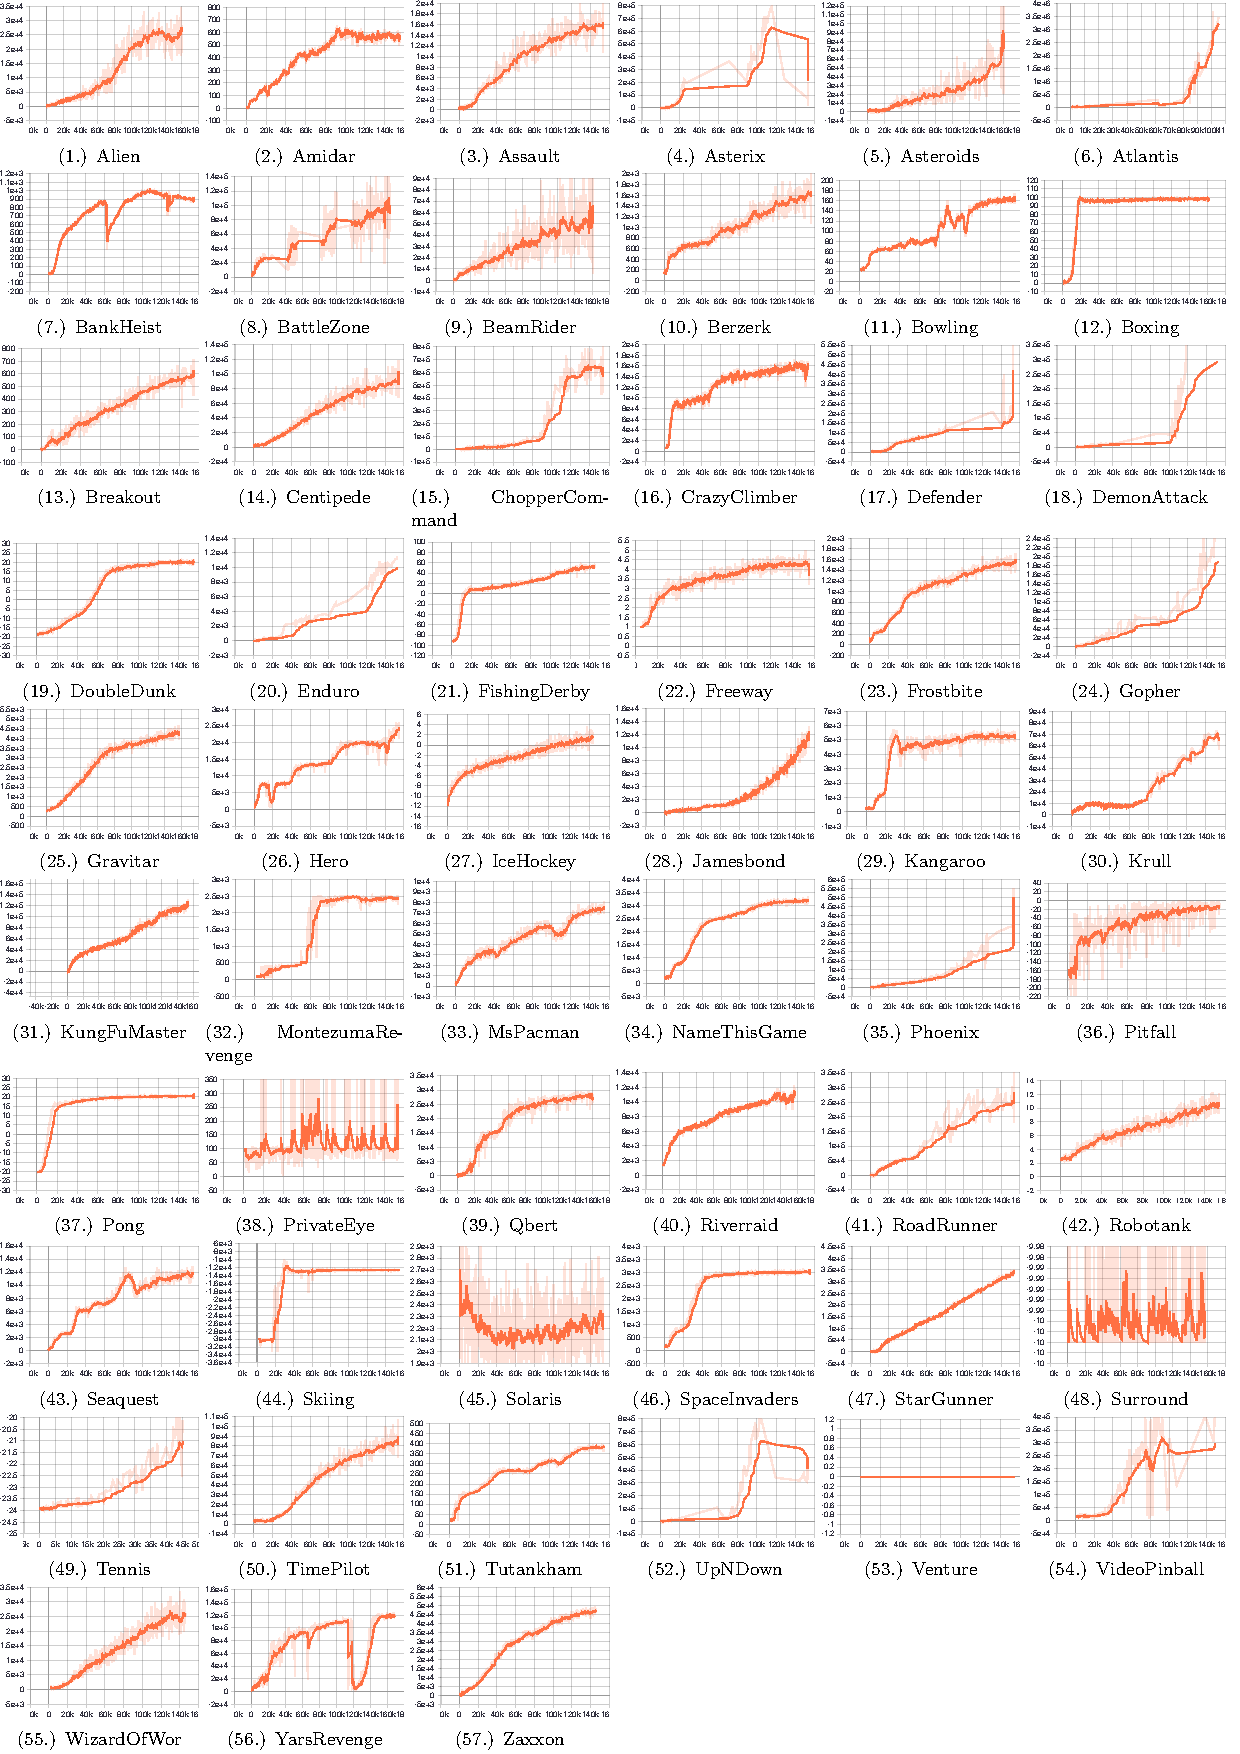
\includegraphics[width=1.0\linewidth]{body/all_fig3.pdf}
\end{figure*}

\clearpage


\fi

\end{document}




\end{document}
